\setcounter{subsection}{0} 
\part{Study of the Monte Carlo cocktail production}
This chapter is devoted to the study of Belle II Monte Carlo cocktail simulations. A Belle II "cocktail" MC production (typically generated with Pythia8) simulates all relevant physics channels simultaneously. Therefore, the analyzed channel $e^+e^- \rightarrow p\pi^-\bar{n}\,(\gamma_\text{ISR})$ is now embedded within all other background channels in the cocktail; the first task is to correctly reconstruct it amidst the surrounding backgrounds, studying the recoil mass distribution.
$\\$
To achieve this, a first attempt uses the $u\bar{u}$ cocktail production. Further selection criteria are developed to properly isolate the signal in the recoil mass distribution.
$\\$
Afterwards, the full Belle II $q\bar{q}$ ($u\bar{u}$, $d\bar{d}$, $c\bar{c}$, $s\bar{s}$) production is analyzed, discussing the corresponding $\bar{n}$ candidates cluster variables.
$\\$
The Feynman diagram of $e^+e^- \rightarrow q \bar{q}$ is shown in Fig.~\ref{fig:Feynman_qqbar}.

\begin{figure}[H]
    \centering
    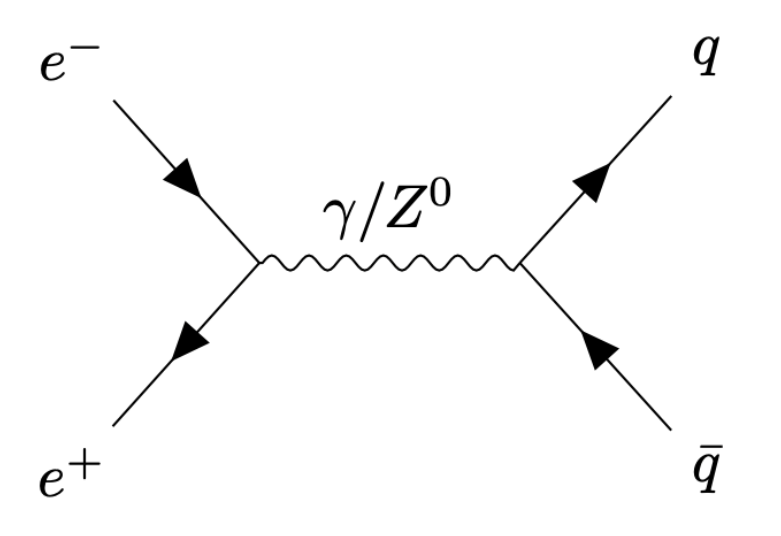
\includegraphics[width=0.45\textwidth]{nbar_cocktail/images/qqbar_diag}
    \caption{Tree level Feynman diagram of $e^+ e^- \to q \bar{q}$}
    \label{fig:Feynman_qqbar}
\end{figure}

\subsection{Types of processes at the Belle experiment enviroment}
Many processes can occur during an $e^+e^-$ collision. These may mimic the selected signal and be accidentally reconstructed as signal events, though they represent background processes.
$\\$
The $\Upsilon(4S)$ production occurs at $\sqrt{s} = 10.58$ GeV, yielding $\Upsilon(4S) \rightarrow BB$ processes. The $B^+B^-$ and $B^0 \bar{B}^0$ final states  are referred to as charged and neutral $B \bar{B}$ pairs, respectively.
$\\$
The $e^+e^- \to q\bar{q}$ ($q = u,d,s,c$) processes, known as continuum production, also occur. There are $e^+e^- \to l^+l^- (\gamma)$ and $e^+e^- \to l^+l^-l^-l^+$, with $l = (e,\mu,\tau)$, that are low multiplicity processes. The cross section distribution \cite{BelleIIPhysicsBook2019} of $e^+ e^- \rightarrow hadrons$ process is shown in Fig.\ref{fig:belleii_processes}.

\begin{table}[h]
\centering
\begin{tabular}{l r}
Process & Cross section (nb) \\
$e^+e^- \to \Upsilon(4S)$ & 1.10 \\
$e^+e^- \to u\bar{u} (\gamma)$ & 1.61 \\
$e^+e^- \to d\bar{d} (\gamma)$ & 0.40 \\
$e^+e^- \to s\bar{s} (\gamma)$ & 0.38 \\
$e^+e^- \to c\bar{c} (\gamma)$ & 1.30 \\
$e^+e^- \to \tau^+\tau^- (\gamma)$ & 0.92 \\
$e^+e^- \to e^+e^- (\gamma)$ & 300 \\
$e^+e^- \to \mu^+\mu^- (\gamma)$ & 1.15 \\
$e^+e^- \to \gamma \gamma (\gamma)$ & 4.99 \\
$e^+e^- \to e^+e^-e^+e^-$ & 39.7 \\
$e^+e^- \to e^+e^-\mu^+\mu^-$ & 18.9 \\
\end{tabular}
\end{table}

\begin{figure}[H]
    \centering
    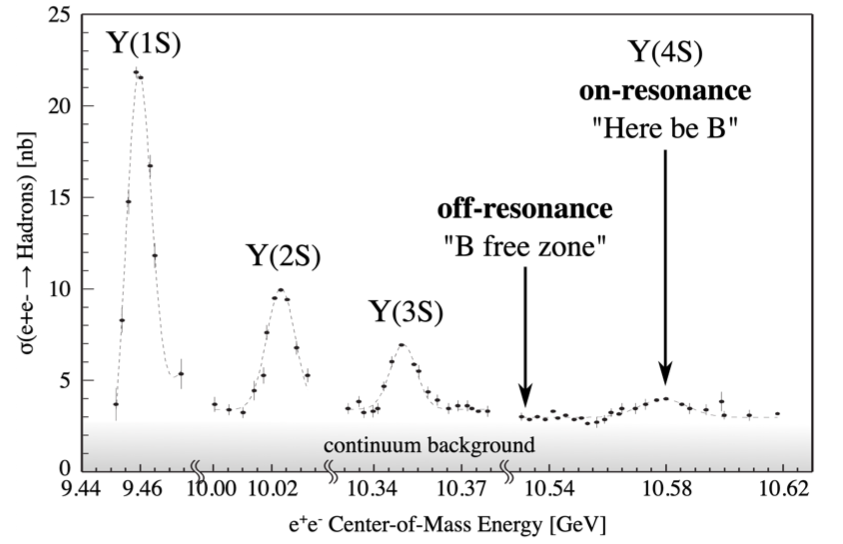
\includegraphics[width=0.9\textwidth]{nbar_cocktail/images/BelleII_processes}
    \caption{Cross section of $e^+ e^- \rightarrow hadrons$, in $\Upsilon$ resonances energy region. The $\Upsilon(1S)$ resonance is very narrow, while the $\Upsilon(4S)$ one is broader and lower.}
    \label{fig:belleii_processes}
\end{figure}

\subsection{Selections criteria}
To follow the same approach as used in the signal sample analysis, the recoil mass is first studied using the complete $u\bar{u}$ cocktail production, which corresponds to an integrated luminosity of $\sim 1429.23 \ fb^{-1}$. The following event selections have been applied:
\begin{enumerate}
\item $p$: $protonID > 0.9$ and $dr<1$ cm and $|dz|<3$ cm;
\item $\pi^-$: $pionID > 0.1$ and $dr<1$ cm and $|dz|<3$ cm;
\item $\bar{n}$: neutral clusters from ECL and number of hits $> 10$ and energy $<3$ GeV;
\item Recoil system: $0 \ GeV/c^2 <recoil \ mass < 2 \ GeV/c^2$;
\item $\alpha <0.20$ rad $\sim 11.5 ^{\circ}$;
\item No further charged particles in the Rest of Event (ROE).
\end{enumerate}
$\\$
Four additional cuts are applied beyond those used for the signal sample, such as cluster number of hits $> 10$ GeV, $\alpha <0.20$ rad, the request of no further charged particles in the Rest of Event (ROE) and the energy of the neutral cluster associated to $\bar{n}$ candidates must be less then 3 GeV.
$\\$
The first cut arises from observations in the previous chapter; to achieve a proper selection of neutral clusters associated with anti-neutron candidates -reducing cluster split-off and pre-showering contributes- a requirement on the number of lighted crystals is applied. 
$\\$
The second cut allows a stricter selection of anti-neutron candidates through a smaller $\alpha$ angle. $\alpha$ is defined as the 3D angle between the recoil vector direction and the neutral cluster associated with the $\bar{n}$. As will be explained later, this threshold can be lowered further.
$\\$
To explain the third cut, the concept of \textbf{Rest of Event} (ROE) must first be introduced. The ROE is built around the reconstructed target particles and consists of all other particles in the Rest of Event. In the present case, the reconstructed particles are $p, \pi^-, \bar{n}$ (and $\gamma_{ISR}$); therefore, the ROE includes all particles outside this reconstructed system. Consequently, the third selection criterion requires that no charged particles -i.e. tracks associated with charged particles- be present in the Rest Of Event, providing a cleaner event reconstruction. A Feynman diagram with ROE is shown in Fig.\ref{fig:ROE_feynman}.

\begin{figure}[H]
    \centering
    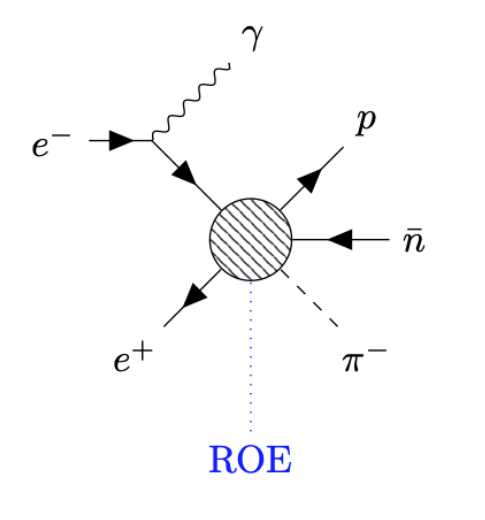
\includegraphics[width=0.45\textwidth]{nbar_cocktail/images/ROE_diag}
    \caption{Feynman diagram of the channel of interest, with the Rest of Event ROE made of a variable amount of particles.}
    \label{fig:ROE_feynman}
\end{figure}

The fourth cut arises from cluster energy studies performed on the first chunk of $u\bar{u}$ cocktail production, corresponding to $\sim 215 fb^{-1}$. The $\bar{n}$ list can be affected by several mis-identified $\gamma_\text{ISR}$. In order to study this phenomenon, the Monte Carlo ISR flag (\textbf{mcISR}) can be used to separate the two contributions in reconstructed $\bar{n}$ list. The mcISR variable is a Monte Carlo flag that indicates whether a particle is an ISR particle or not;
if mcISR = 0, the reconstructed particle is not an ISR photon; if mcISR = 1, the reconstructed particle is an ISR photon mis-identified as an anti-neutron. The obtained cluster energy distribution for $\bar{n}$ candidates, in $u\bar{u}$ chunk1 cocktail production, is shown in figure ~\ref{fig:E_isr_uubar_c1}.
$\\$
Two structures, at $\sim 4$ GeV and $\sim 6$ GeV, due to $\gamma_{ISR}$ mis-identified as anti-neutrons, arise. In order to remove them, a cut on cluster energy, such as those discussed, is mandatory.
\begin{figure}[h]
    \centering
    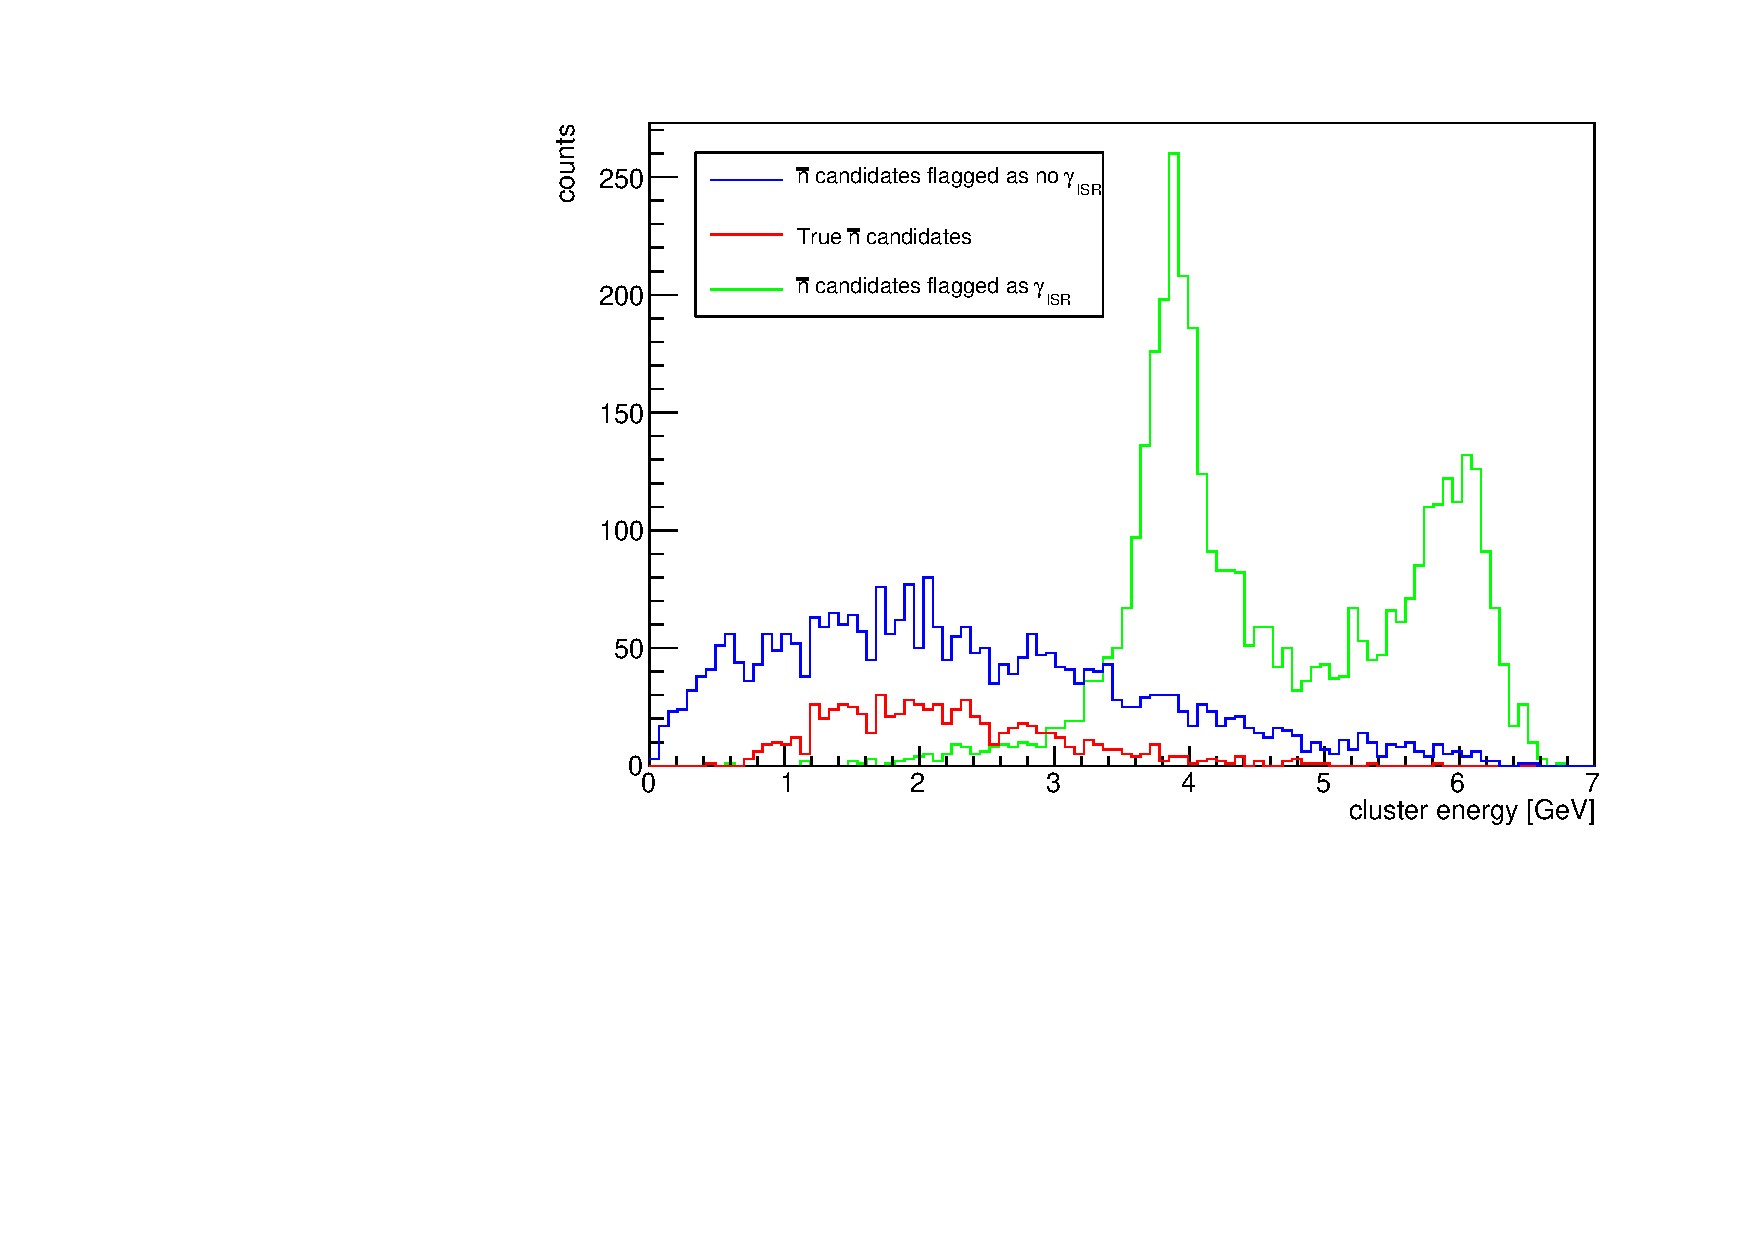
\includegraphics[width=0.80\textwidth]{nbar_cocktail/images/clusterEnergy_isr}
    \caption{Cluster energy distribution of $\bar{n}$ candidates, divided by the Monte Carlo ISR flag (\texttt{mcISR}), in $u\bar{u}$ chunk1 cocktail production. If \texttt{mcISR} = 0 (blue), the reconstructed particle is not an ISR photon. If \texttt{mcISR} = 1 (red), the reconstructed particle is an ISR photon. \texttt{mcISR} is a Monte Carlo information.}
    \label{fig:E_isr_uubar_c1}
\end{figure}
$\\$
However, $\gamma$ radiation represents one of the most abundant produced particles in HEP experiments such as Belle II, making a major contribution to the background. In addition to the ISR ($E \sim 10$ MeV - $5$ GeV, Fig.~\ref{fig:isr_distro}) and FSR ($E< 10$ MeV) radiation described above, bremsstrahlung ($E < 50$ MeV) and secondary photons -such as those from $\pi^0 \rightarrow \gamma \gamma$ decays  ($E < 400$ MeV)- are also present. Therefore, NO ISR channel where the recoil system is made of  $p, \pi^-$ should represents a cleaner system to reconstruct than the ISR one where the recoil system is made of  $p, \pi^-, \gamma$, since several background $\gamma$'s can be mis-identified as the ISR photon, which must be accounted for in the recoil system.
$\\$
In order to compare the feasibility of selecting the channel in both ISR and NO ISR cases separately, the recoil mass distribution must be first studied using the same selection criteria. The better the selection of the signal from the background, the more consistent the shower shape variables will be for neutral clusters associated with $\bar{n}$ candidates.

\subsection{Recoil mass in $u\bar{u}$ cocktail production (NO ISR case)}
The recoil mass distribution obtained from the $u\bar{u}$ cocktail is first studied in NO ISR case. If the recoil system $p, \pi^-$ is properly reconstructed among all possible background channels, then a peak should be observed at the anti-neutron rest mass ($939.5$~MeV/$c^2$). The obtained result is shown in Fig.~\ref{fig:mRec_nog_020}.
\begin{figure}[h]
    \centering
    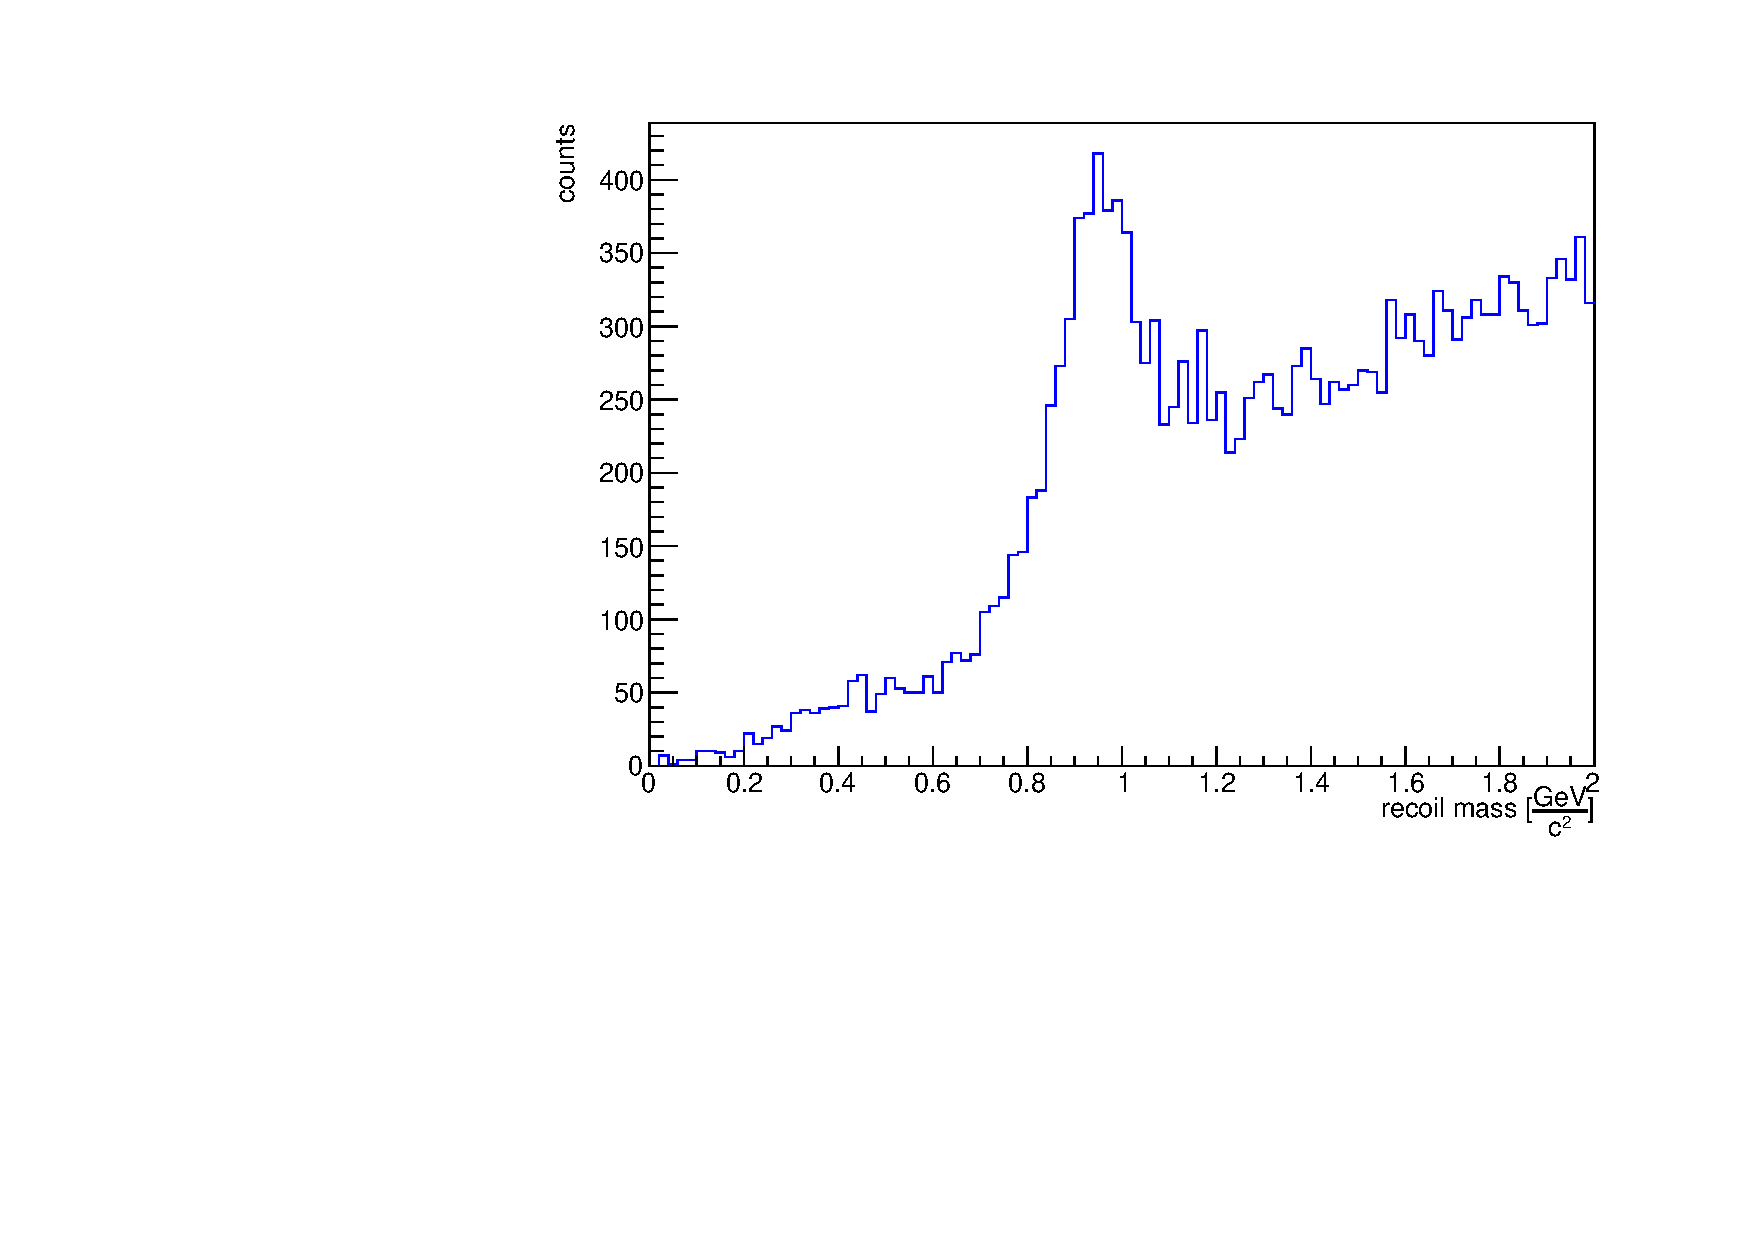
\includegraphics[width=0.80\textwidth]{nbar_cocktail/images/recoil_mass_nog_020}
    \caption{Reconstructed $p, \pi^-$ recoil mass distribution in $u\bar{u}$ Monte Carlo cocktail, NO ISR case.}
    \label{fig:mRec_nog_020}
\end{figure}

A distinct structure is observed above the $\bar{n}$ mass value, suggesting that the selected channel is properly reconstructed. For a cleaner comparison between the signal channel and background components, the TopoAna output can be consulted in Fig.~\ref{fig:topo_nog_020}. TopoAna does not account for particle-matter interactions; thus, all displayed particles originate directly from the $e^+e^-$ collision at the IP.
\begin{figure}[h]
    \centering
    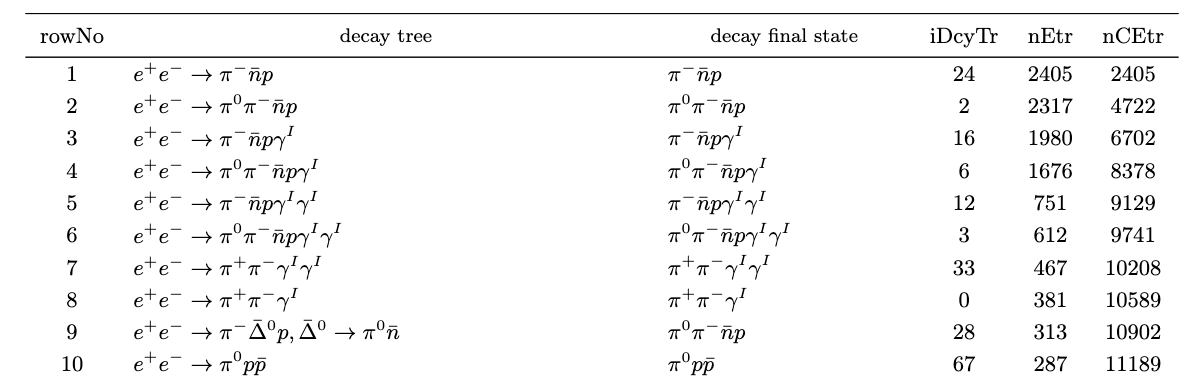
\includegraphics[width=1\textwidth]{nbar_cocktail/images/topoana_nog_020}
    \caption{First 10 channels of the TopoAna output in $u\bar{u}$ Monte Carlo cocktail, showing the different channel contributes, NO ISR case.}
    \label{fig:topo_nog_020}
\end{figure}

Accessing the Monte Carlo information from TopoAna, the main contribution comes from the signal channel with $p \pi^- \bar{n}$ in the final state, immediately followed by the one with $p \pi^- \bar{n} \pi^0$ in the final state. Further contribution arise from $p \pi^- \bar{n} \gamma_{ISR}$, which could be interpreted as signal, even if, in NO ISR case, the $\gamma_{ISR}$ is not explicitly reconstructed within the recoil system. The fourth contribute is due to the one with $p \pi^- \bar{n} \pi^0 \gamma_{ISR}$ and so on. The contributions are sorted from most to least abundant.

\subsubsection{Recoil mass components analysis}
The recoil mass distribution components can be studied by correlating the ntuple information obtained from the steering file with that produced by the TopoAna program. 
$\\$
Each channel is identified by its own \texttt{iDcyTr} (index of the decay tree), which allows one to represent the contribution of a given channel (or a combination of channels) to a specific variable, such as the recoil mass of the system $p \pi^-$.
$\\$
The components are therefore denoted as follows:
\begin{enumerate}
\item $e^+ e^- \rightarrow \pi^- \bar{n} p$ (iDcyTr == 24);
\item $e^+ e^- \rightarrow \pi^0 \pi^- \bar{n} p$ (iDcyTr == 2);
\item $e^+ e^- \rightarrow \pi^- \bar{n} p \gamma_{ISR}$ (iDcyTr == 16);
\item $e^+ e^- \rightarrow \pi^0 \pi^- \bar{n} p \gamma_{ISR}$ (iDcyTr == 6);
\item $e^+ e^- \rightarrow$ other.
\end{enumerate}
The obtained stacked component to the recoil mass are shown in figure ~\ref{fig:mRecComps_nog_020}.
\begin{figure}[h]
    \centering
    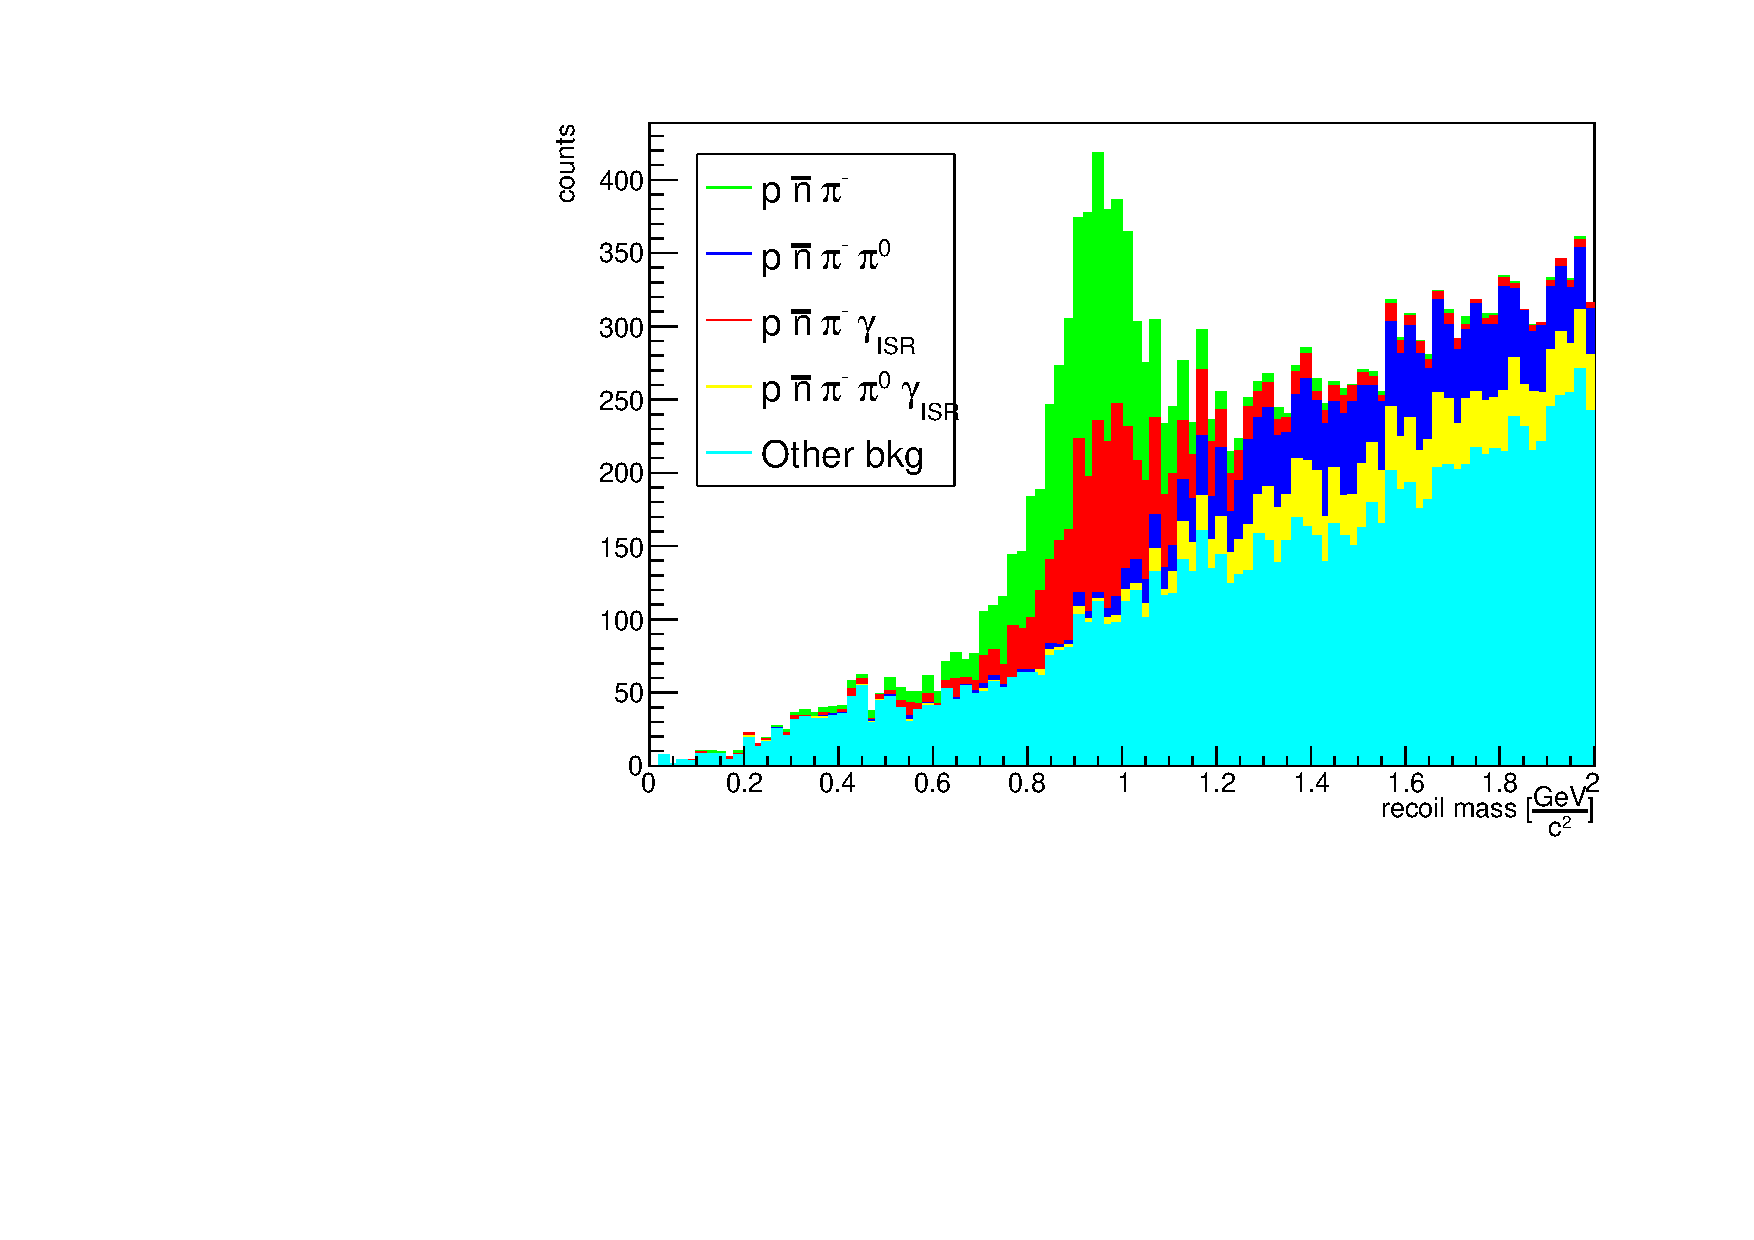
\includegraphics[width=0.90\textwidth]{nbar_cocktail/images/recoilM_comps_nog_020}
    \caption{$p, \pi^-$ recoil mass distribution in $u\bar{u}$ Monte Carlo cocktail, displaying each stacked component contribution, NO ISR case. Green: $\pi^- \bar{n} p$ channel. Blue: $\pi^0 \pi^- \bar{n} p$ channel. Red: $\pi^- \bar{n} p \gamma_{ISR}$. Yellow: $\pi^0 \pi^- \bar{n} p \gamma_{ISR}$ channel. Cyan: other channels.}
    \label{fig:mRecComps_nog_020}
\end{figure}
Defining the \emph{Signal Region} as the interval $[0.8, 1.2]$ GeV, it can be observed that contributions from the channel with iDcyTr = 2 predominantly lie to the right of the signal region. This is expected, as the recoil system computation excludes the $\pi^0$, leading to a higher recoil mass. Same conclusions can be made for the with iDcyTr = 6. 
$\\$
The signal channel (iDcyTr = 24) predominantly populates the signal region. The $\pi^- \bar{n} p \gamma_{ISR}$ channel (iDcyTr = 16) also mainly populates the signal region, indicating that the $\gamma_{ISR}$ is negligible and has minimal impact on the recoil mass, as shown by the ISR energy distribution in Fig.~\ref{fig:isr_distro}. This can be directly observed from the single contribute from these two channels displayed in Fig.~\ref{fig:mRecComps_nog_020_0e3}. The contributions from the remaining channels represent a flat background without discernible structures.
\begin{figure}[H]
    \centering
    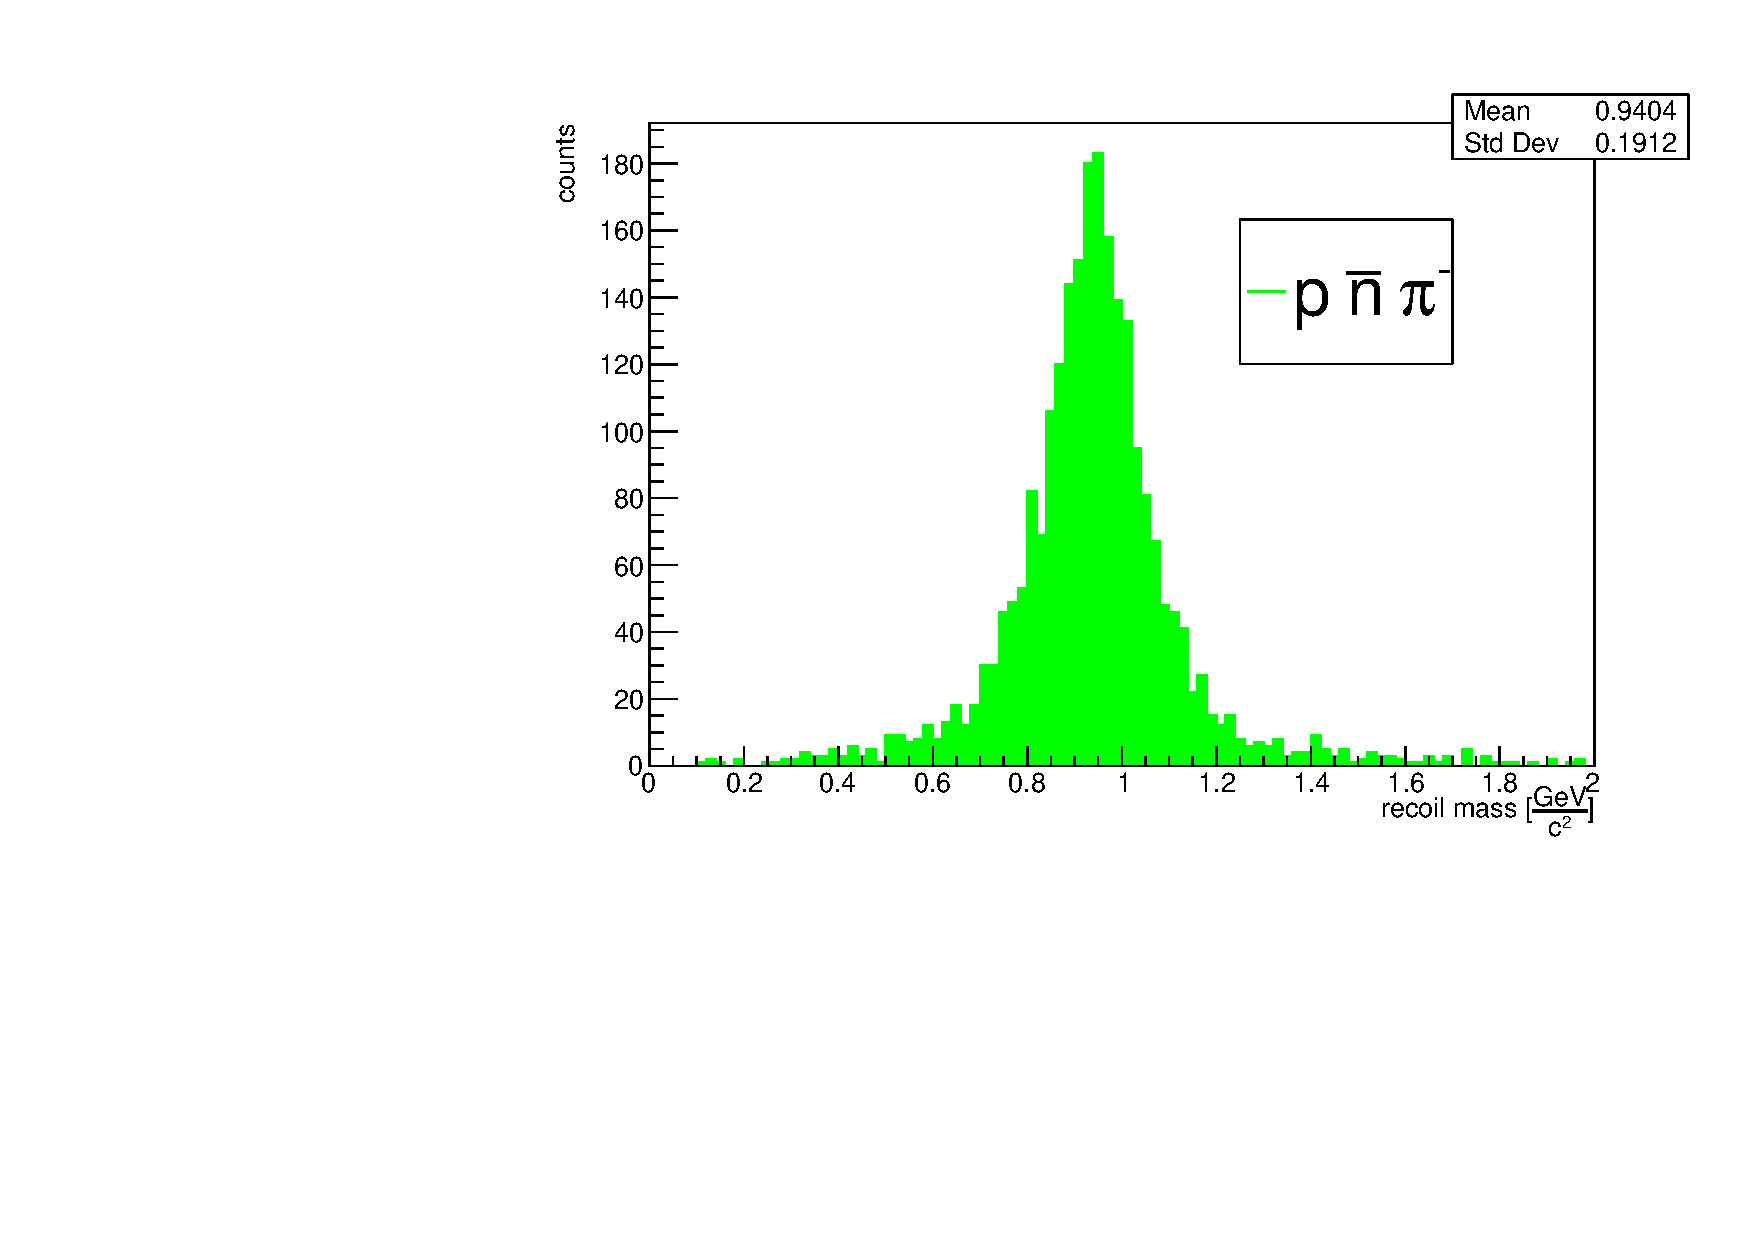
\includegraphics[width=0.49\textwidth]{nbar_cocktail/images/recoilM_comp0_nog_020}
    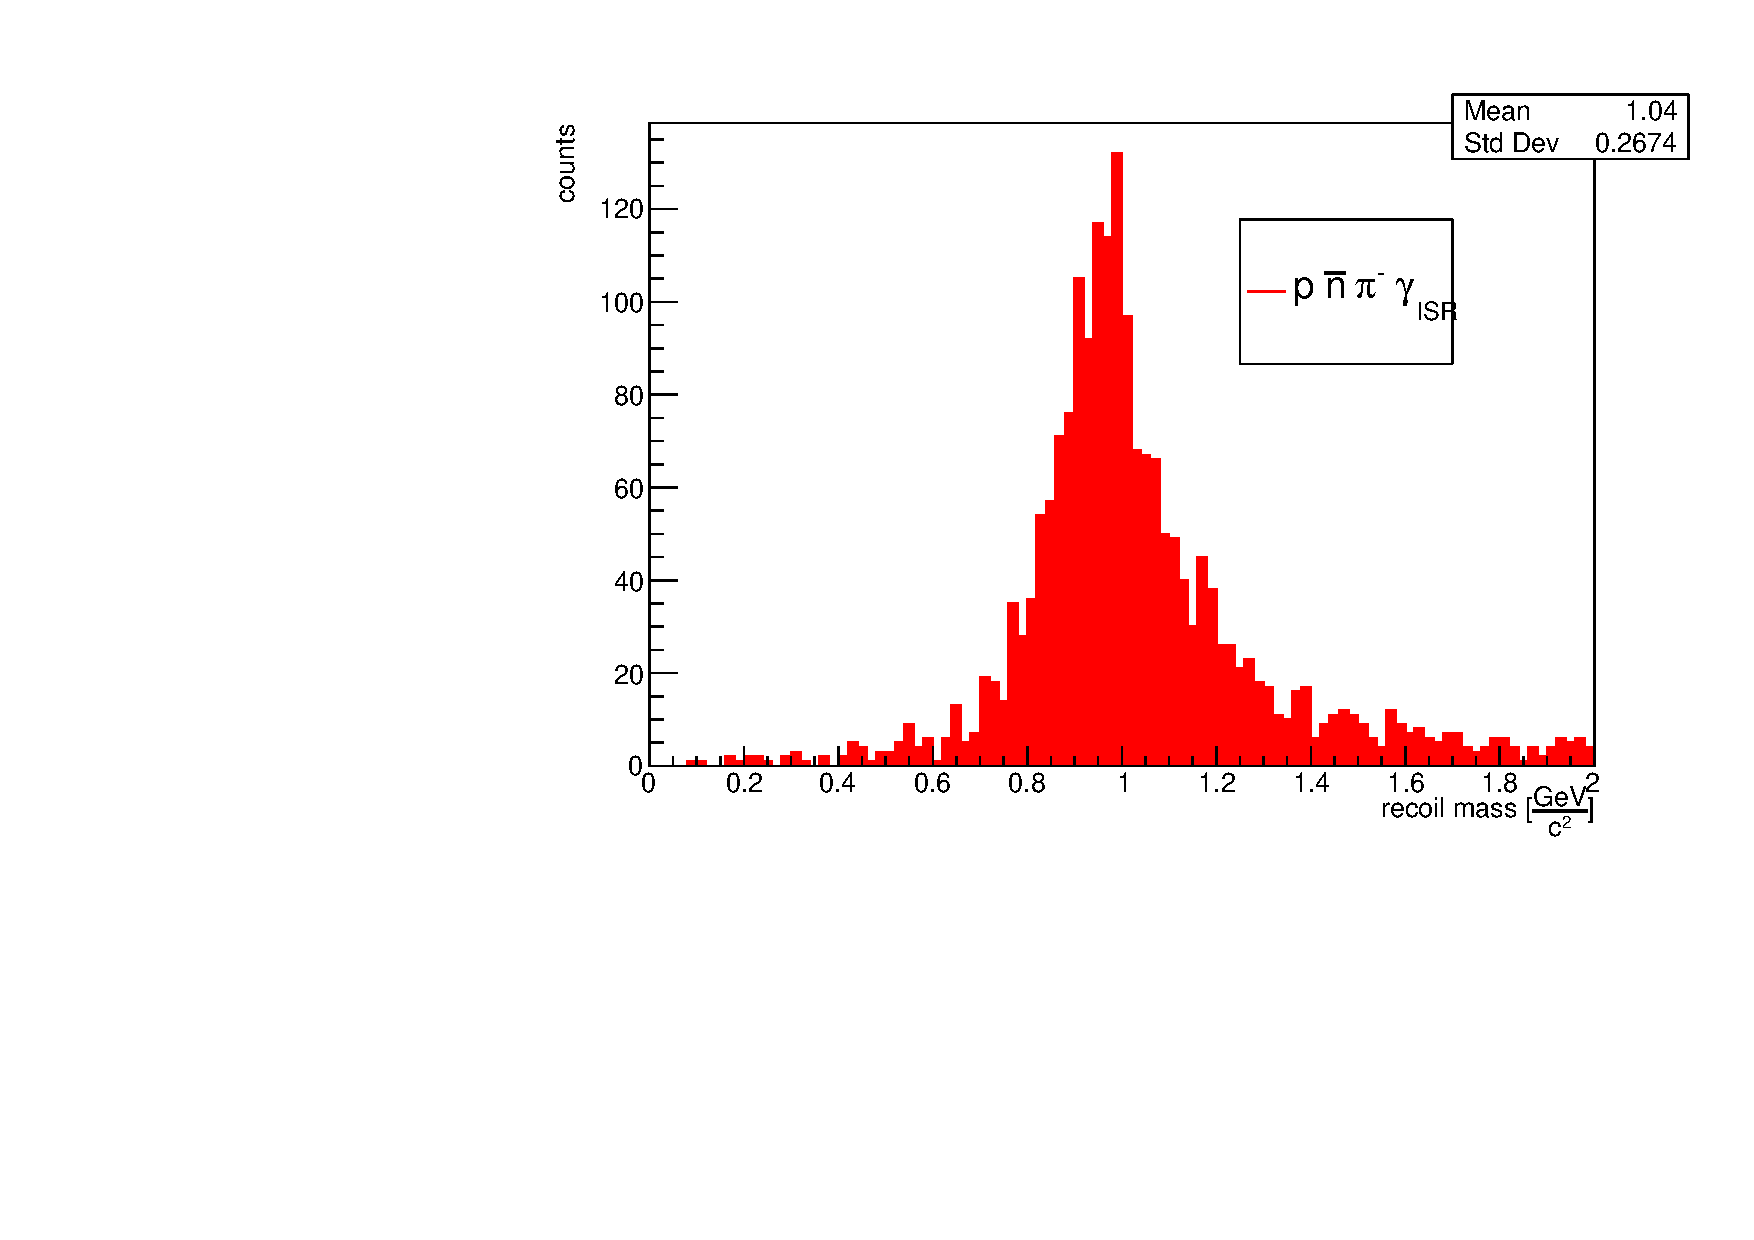
\includegraphics[width=0.49\textwidth]{nbar_cocktail/images/recoilM_comp3_nog_020}
    \caption{ (green) $p, \pi^-$ recoil mass and (red) $p, \pi^-, \gamma_{ISR}$ recoil mas distribution in $u\bar{u}$ Monte Carlo cocktail.}
    \label{fig:mRecComps_nog_020_0e3}
\end{figure}
$\\$
Thus, despite the $\gamma_{ISR}$ not being directly reconstructed, the $\pi^- \bar{n} p \gamma_{ISR}$ channel (iDcyTr = 16) can be considered a signal channel. This leads to the recoil mass composition shown in Fig.~\ref{fig:mRecComps_nog_020_0+3}.
\begin{figure}[h]
    \centering
    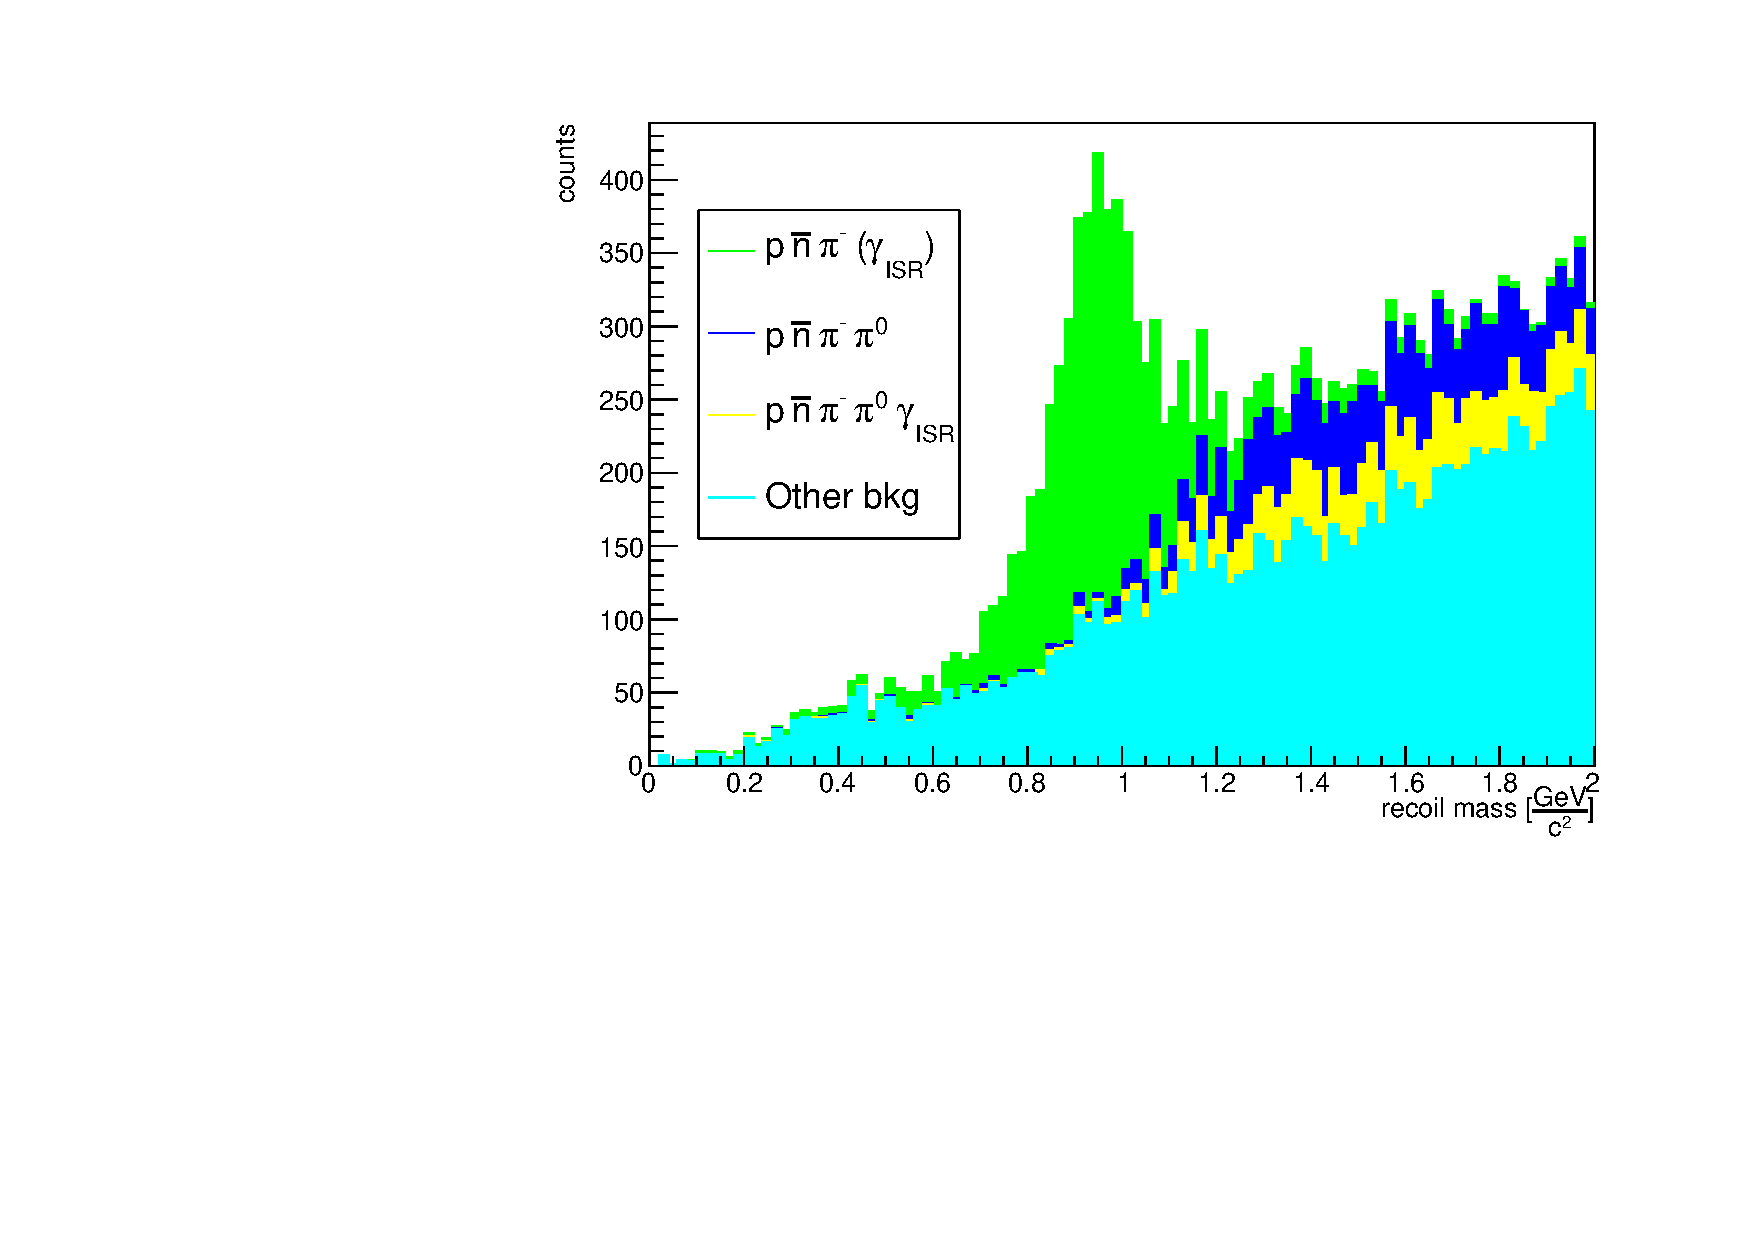
\includegraphics[width=0.90\textwidth]{nbar_cocktail/images/recoilM_comps_nog_020_0+3}
    \caption{$p, \pi^-$ recoil mass distribution in $u\bar{u}$ Monte Carlo cocktail, displaying each stacked component contribution, NO ISR case. Green: $\pi^- \bar{n} p$ and $\pi^- \bar{n} p \gamma_{ISR}$ channels. Blue: $\pi^0 \pi^- \bar{n} p$ channel. Yellow: $\pi^0 \pi^- \bar{n} p \gamma_{ISR}$ channel. Cyan: other channels.}
    \label{fig:mRecComps_nog_020_0+3}
\end{figure}
$\\$
To further suppress the background, a tighter $\alpha$ cut can be studied. Therefore, the Performance Metrics and their usage are investigated to find the most appropriate cut in $\alpha$.

\subsubsection{Performance Metrics study on $\alpha$ cut}
In general, a \textbf{Performance Metric} quantifies how a classification process is optimized based on a specific parameter, which could, for example, be represented by a threshold.
$\\$
In this specific HEP context, a performance metric quantifies how well the selection cuts distinguish the signal from the background. In this analysis, the signal can be assumed to be the channel with  $\pi^- \bar{n} p (\gamma_{ISR})$ in the final state, while the background is represented by all the other channels. Therefore, a stricter cut on the $\alpha$ angle is investigated to determine whether it improves signal selection over background.
$\\$
To address this kind of analysis, performance metrics such as the \textbf{Figure of Merit} (FOM), the Signal Efficiency ($\epsilon_{sig}$), the Background Efficiency ($\epsilon_{bkg}$) and the \textbf{purity} can be employed. These are defined as follow:
\begin{itemize}
\item FOM = $\frac{SIGNAL(\alpha)}{\sqrt{SIGNAL(\alpha) + BACKGROUND(\alpha)}}$;
\item $ \epsilon_{sig}  = \frac{SIGNAL(\alpha)}{SIGNAL(\alpha = 0.20 \ rad)}$;
\item $ \epsilon_{bkg}  =  \frac{BACKGROUND(\alpha)}{BACKGROUND(\alpha = 0.20 \ rad)}$;
\item Purity $= \frac{SIGNAL(\alpha)}{SIGNAL (\alpha)+ BACKGROUND(\alpha)}$.
\end{itemize}
SIGNAL and BACKGROUND are defined as follows:
\begin{itemize}
 \item SIGNAL($\alpha$) is defined by the number of entries from the signal channel, depending on $\alpha$;
 \item BACKGROUND($\alpha$) is defined by the number of entries from the other channels within the signal region, depending on $\alpha$.
 \end{itemize}
SIGNAL($\alpha$) + BACKGROUND ($\alpha$) = TOTAL($\alpha$), the total  amount of entries.
$\\$
Assuming the signal region corresponds to the interval $[0.8, 1.2]$ GeV, the FOM characterizes the statistical significance of the applied threshold, namely the selected cut on $\alpha$. The higher the FOM, the more signal is selected over the background (the figure is maximized). For each possible cut value of $\alpha$, the Figure of Merit (FOM) is computed and the cut corresponding to the maximum FOM (or to a stable plateau) is selected. A higher FOM indicates a better trade-off between signal efficiency and background rejection, so the selection is optimized when the FOM is maximized. The obtained FOM is shown in Fig.~\ref{fig:fom_alpha020}.
\begin{figure}[h]
    \centering
    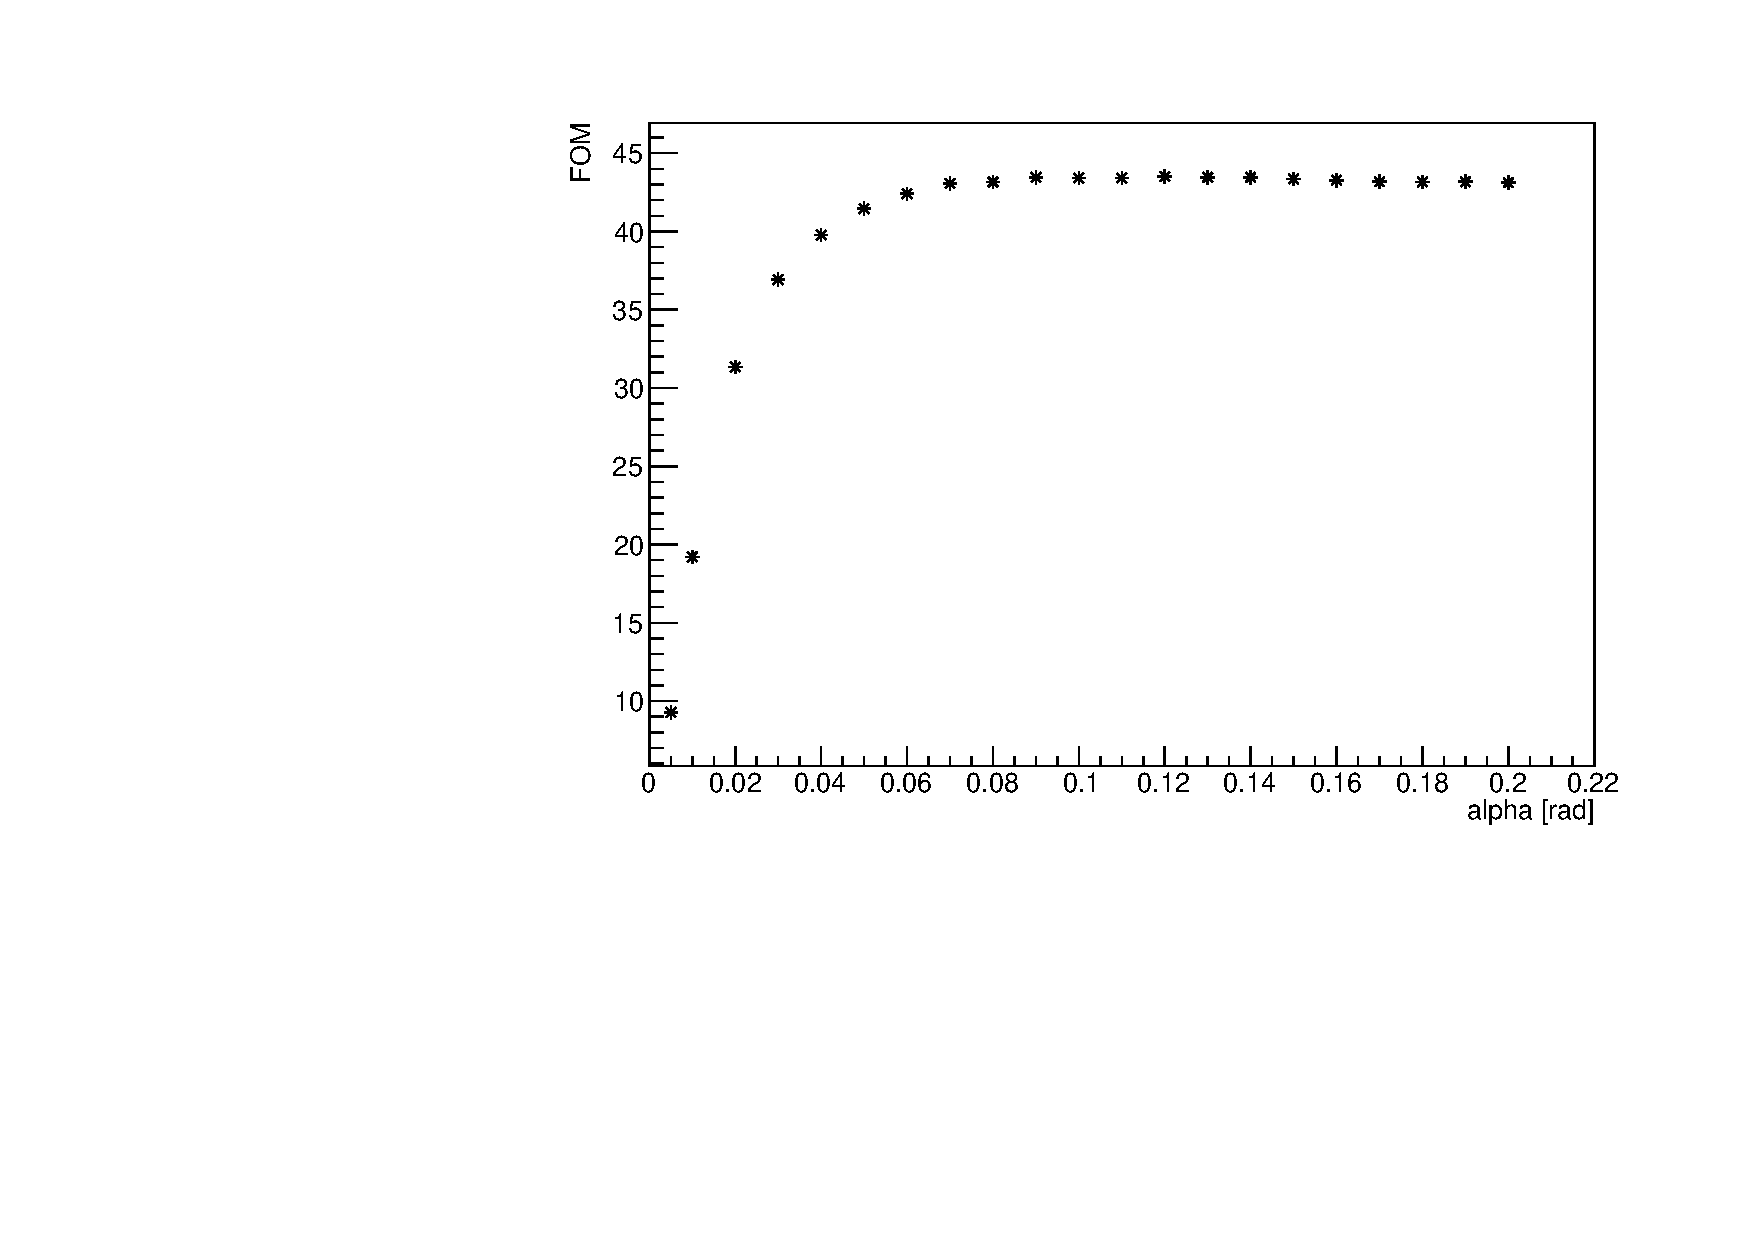
\includegraphics[width=0.70\textwidth]{nbar_cocktail/images/fom_alpha}
    \caption{Figure of Merit (FOM) versus $\alpha$ angle for the $u\bar{u}$ cocktail.}
    \label{fig:fom_alpha020}
\end{figure}
$\\$
One $\alpha$ value corresponding to the plateau can be chosen in order to maximize the FOM. The value $\alpha < 0.1$ rad ($\sim 5.73^\circ$) is therefore chosen, corresponding to FOM = 43.4185
$\\$
Furthermore, the signal efficiency $\epsilon_{sig}$ and the background efficiency $\epsilon_{bkg}$ performance metrics can be adopted to study the Receiver Operating Characteristic (ROC), a curve that shows how well a binary classifier distinguishes signal from background as the decision threshold ($\alpha$ cut) is varied.
Each point on the curve corresponds to a different threshold (a cut on the $\alpha$ angle). The Area Under the ROC Curve (AUC/ROC-AUC) is a single number summarizing the overall performance: 1.0 indicates perfect discrimination, while 0.5 corresponds to no better performance than random. The obtained ROC is shown in Fig.~\ref{fig:roc_alpha020}.
\begin{figure}[H]
    \centering
    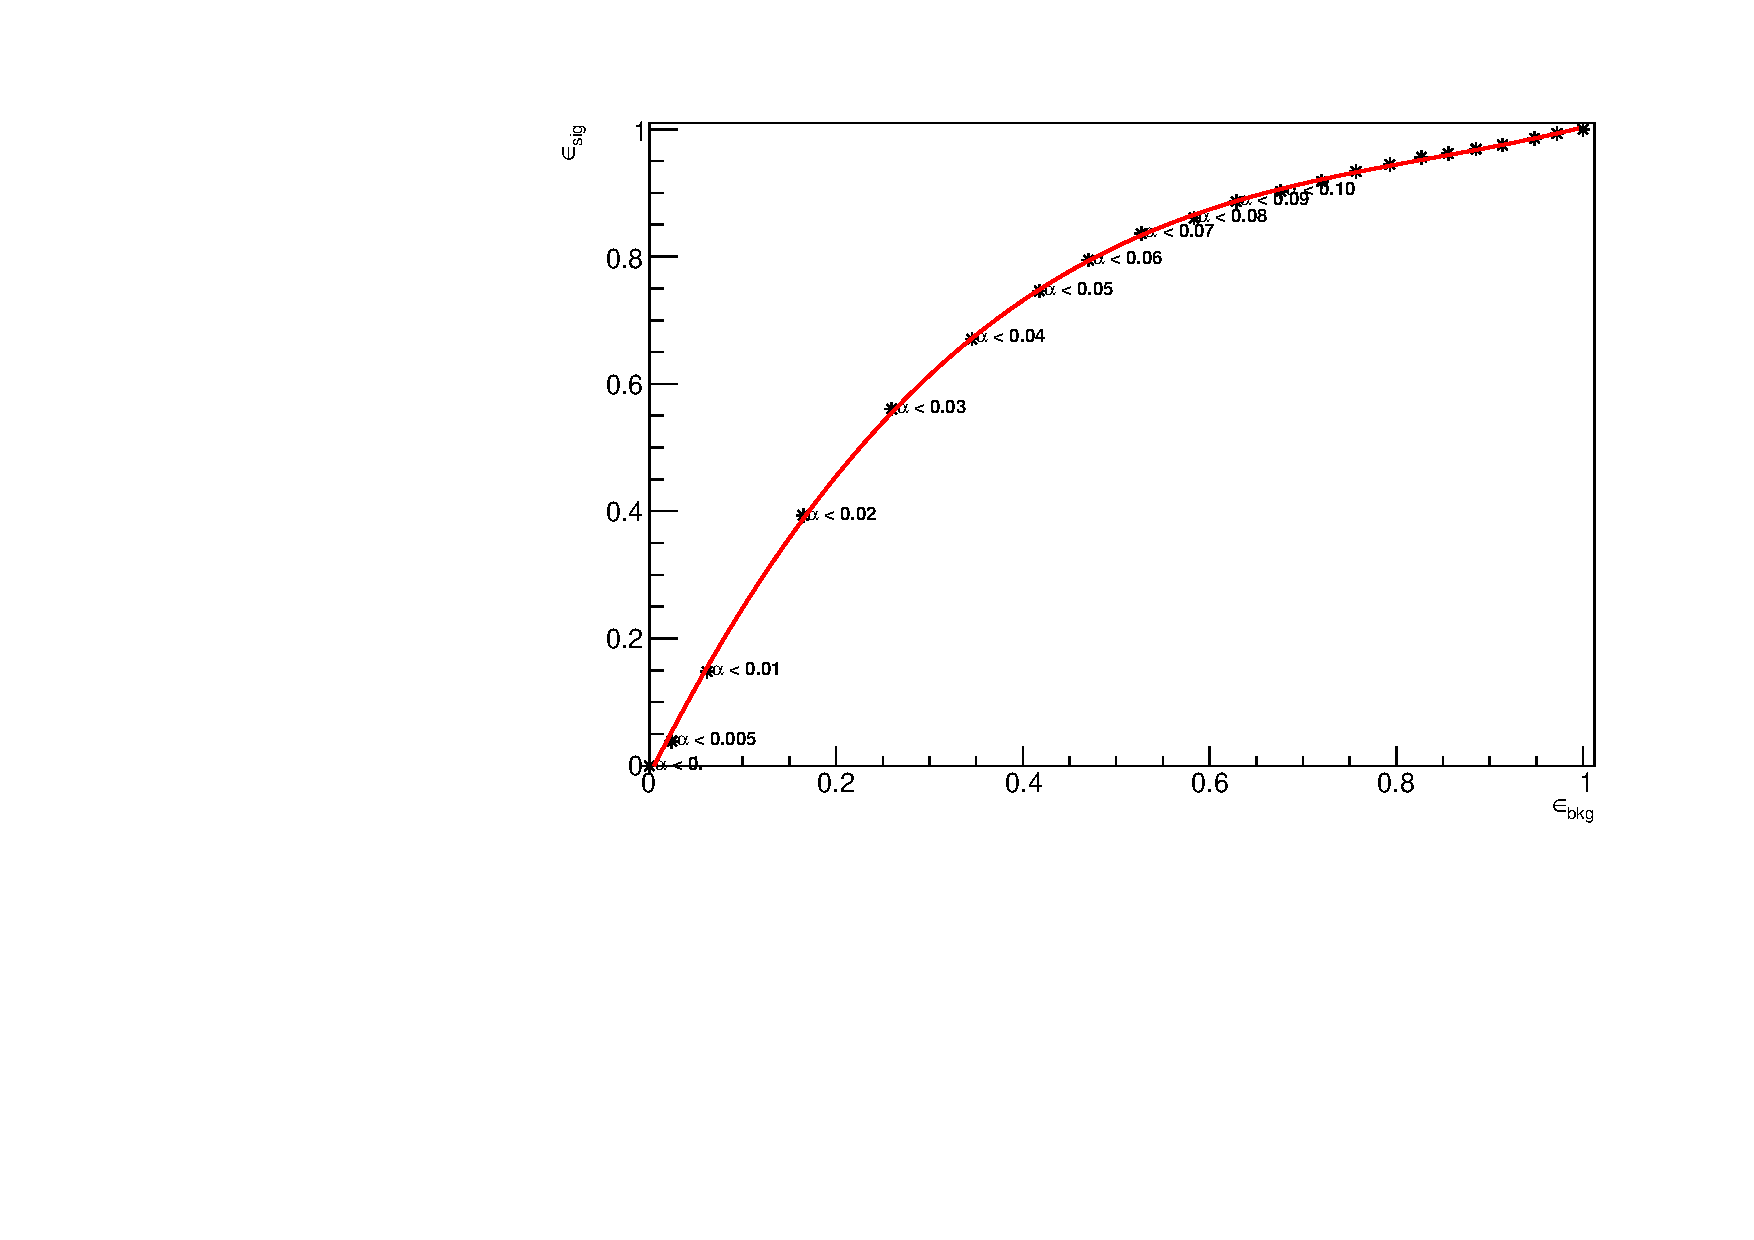
\includegraphics[width=0.70\textwidth]{nbar_cocktail/images/roc_alpha_true}
    \caption{Receiver Operating Characteristic (ROC) curve constructed from the signal efficiency ($\epsilon_{sig}$) and the Background Efficiency ($\epsilon_{bkg}$), where each point corresponds to a different cut value on the $\alpha$ angle. The labels are shown only for $\alpha < 0.10$ rad.}
    \label{fig:roc_alpha020}
\end{figure}

The Receiver Operating Characteristic (ROC) curve for the $\alpha$ angle cut yields an area under the curve (AUC) of $0.71$, indicating good discrimination power between signal and background.
$\\$
Therefore, the obtained performance metrics for $\alpha < 0.1$ rad are:
\begin{center}
$FOM = 43.4185$, $\epsilon_{sig}= 90\%$, $\epsilon_{bkg}= 68\%$,  $Purity = 63\%$
\end{center}
The obtained $\epsilon_{sig}$ vs $Purity$ is shown in Fig.~\ref{fig:eff_alpha020}.
\begin{figure}[H]
    \centering
    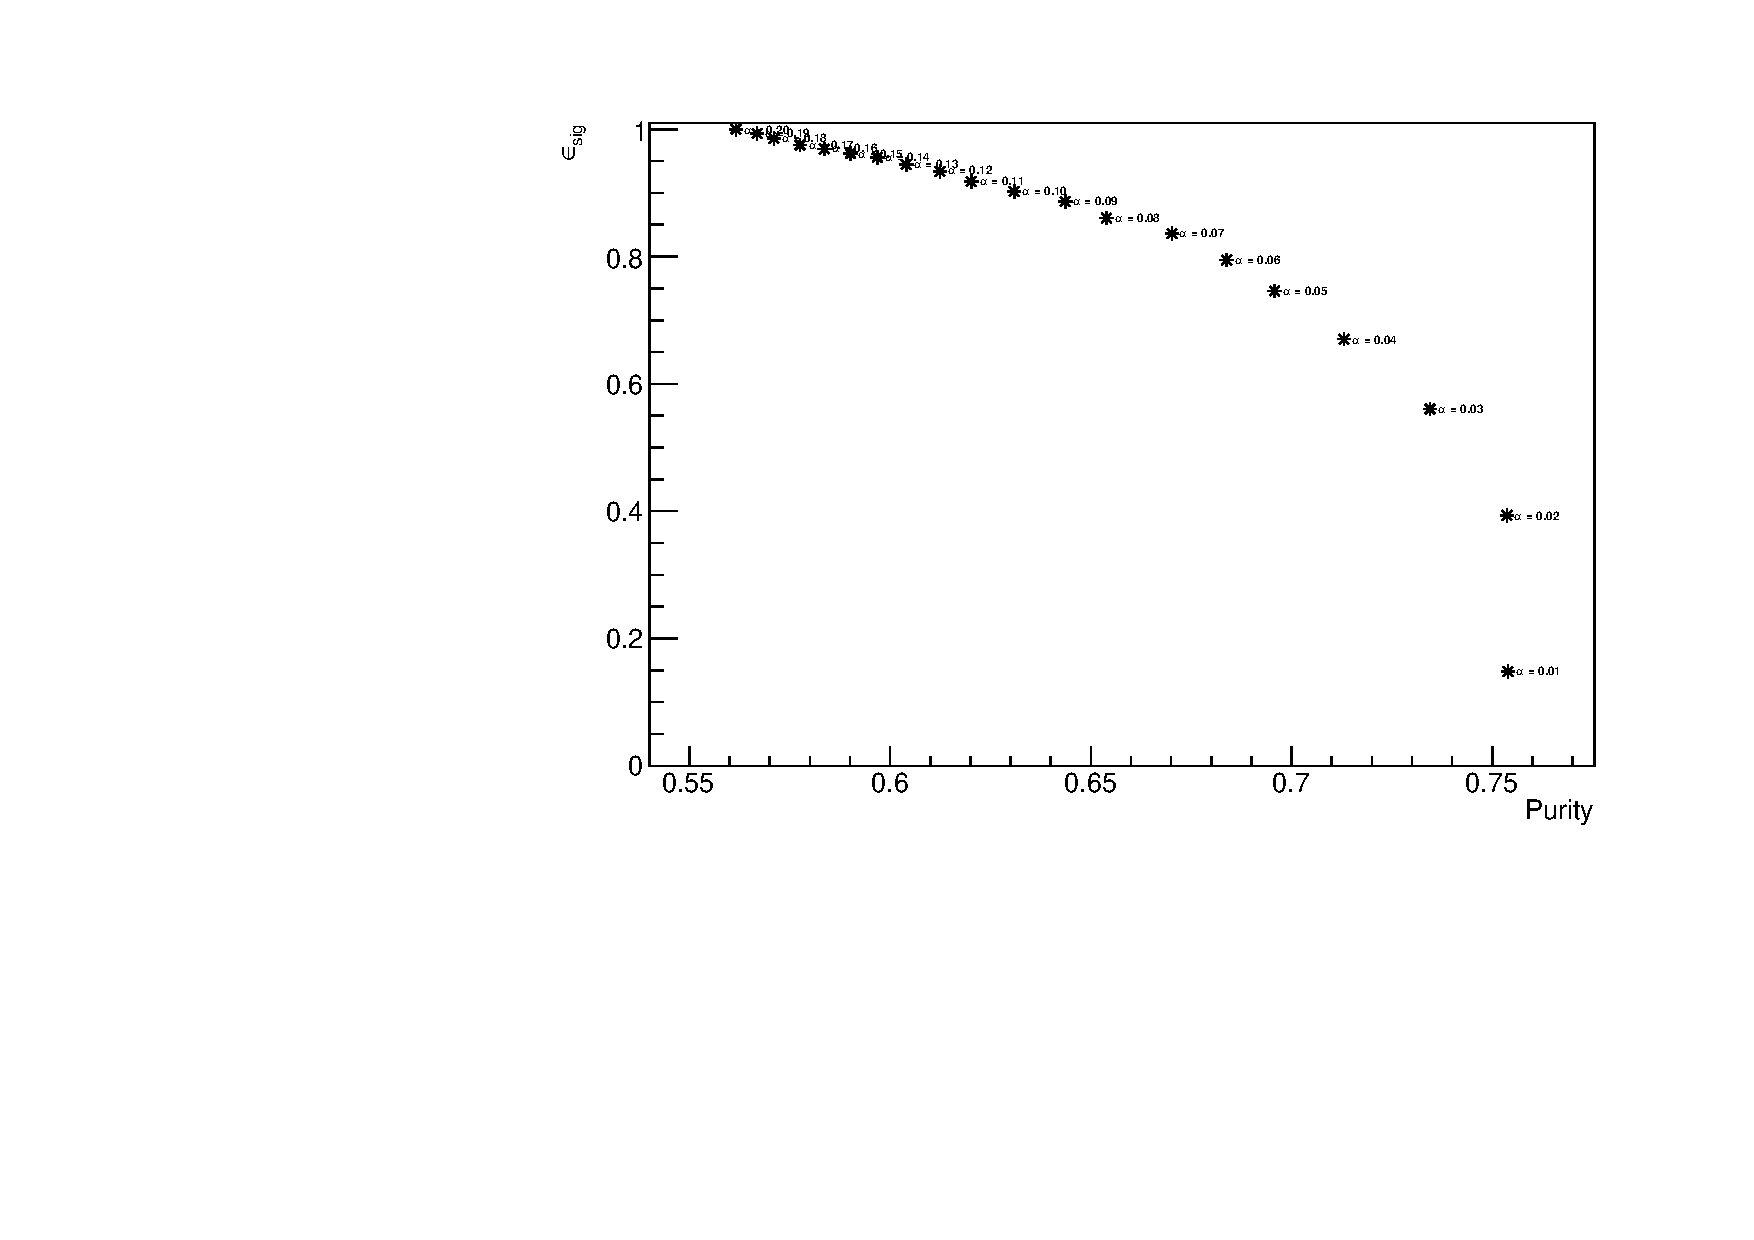
\includegraphics[width=0.70\textwidth]{nbar_cocktail/images/eff_alpha}
    \caption{ $\epsilon_{sig}$ vs $Purity$ curve for the $u\bar{u}$ Monte Carlo cocktail.}
    \label{fig:eff_alpha020}
\end{figure}
Following the described optimization, the recoil mass channel components distribution can now be analyzed using the cut $\alpha < 0.10$ rad.
$\\$
The obtained stacked component to the recoil mass are shown in Fig.~\ref{fig:mRecComps_nog_010}.
\begin{figure}[h]
    \centering
    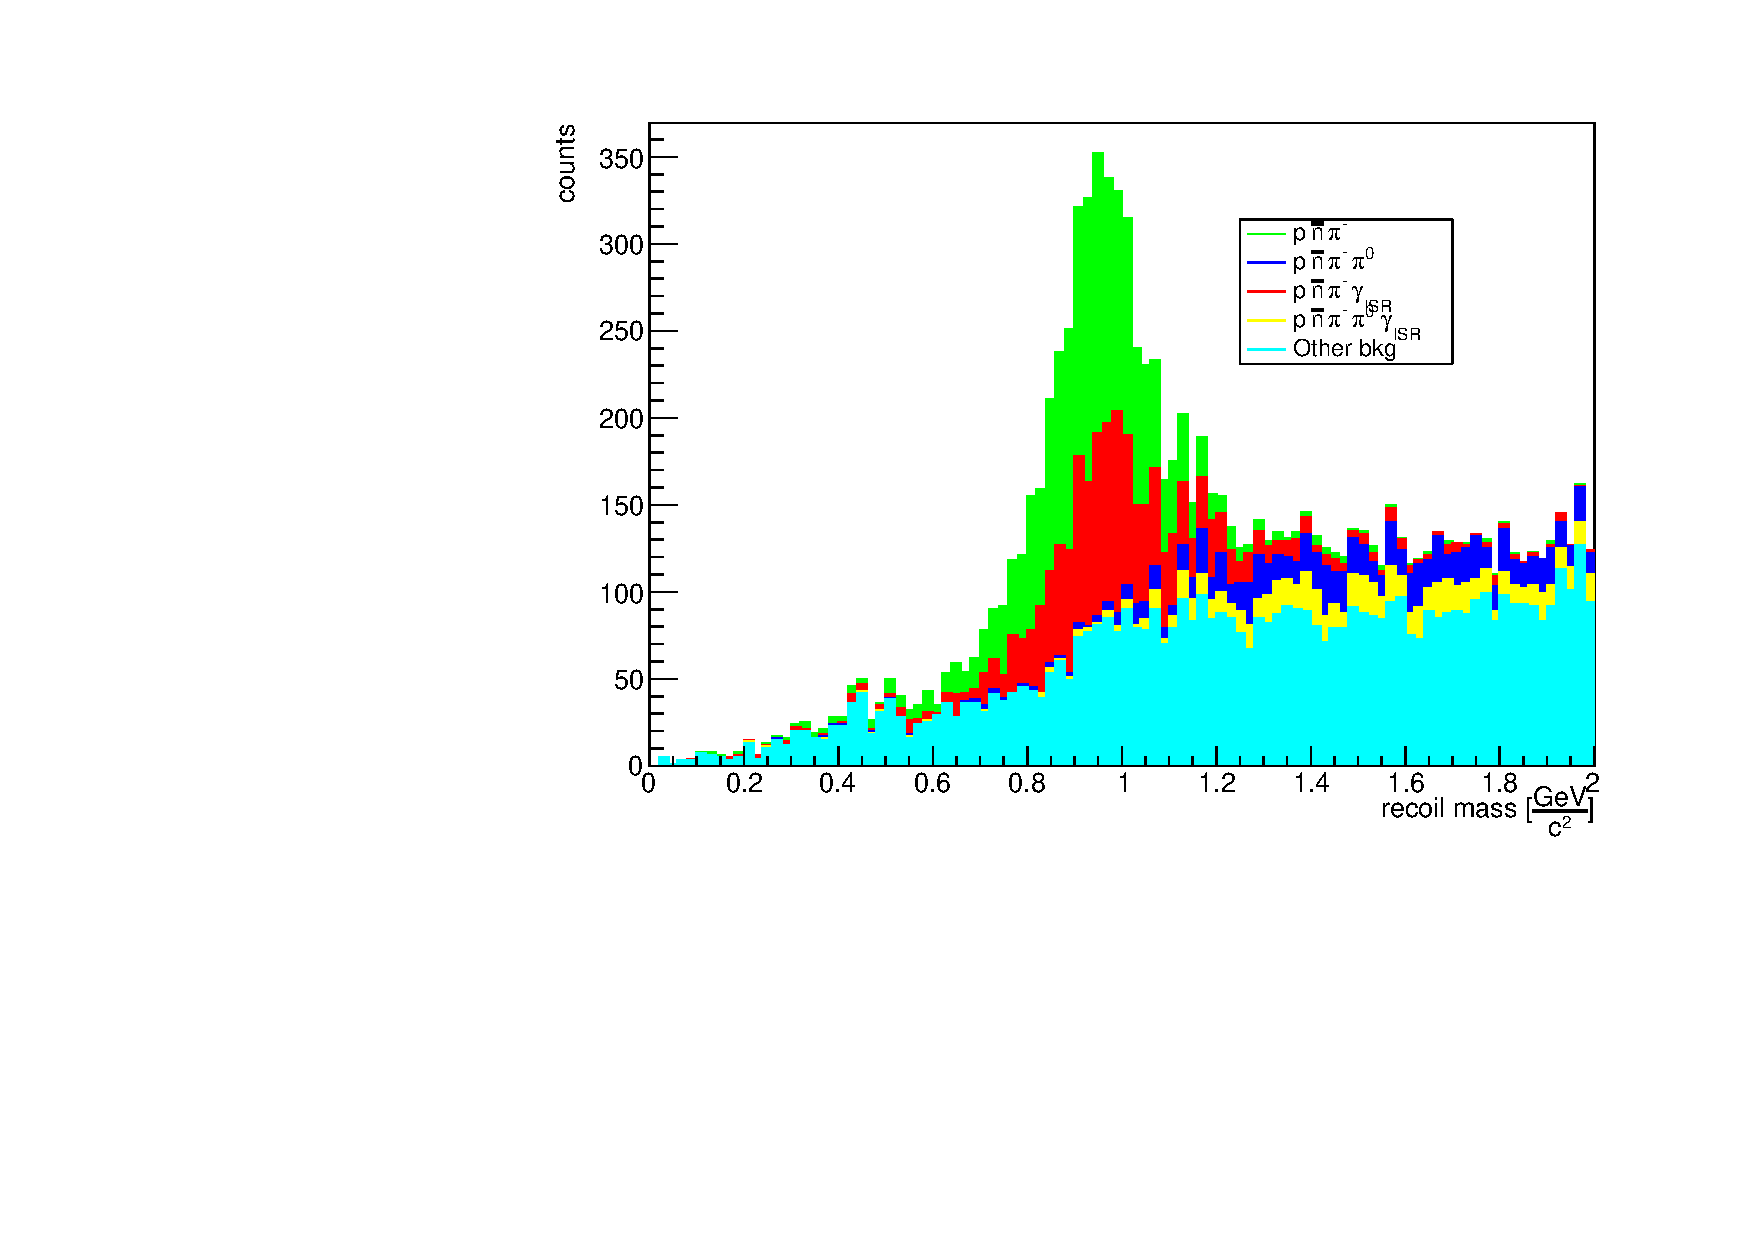
\includegraphics[width=0.8\textwidth]{nbar_cocktail/images/recoilM_comps_nog_010}
    \caption{$p, \pi^-$ recoil mass distribution, displaying each stacked component contribution, NO ISR case. Green: $\pi^- \bar{n} p$ channel. Blue: $\pi^0 \pi^- \bar{n} p$ channel. Red: $\pi^- \bar{n} p \gamma_{ISR}$. Yellow: $\pi^0 \pi^- \bar{n} p \gamma_{ISR}$ channel. Cyan: other channels. $\alpha<$ 10 rad cut is applied.}
    \label{fig:mRecComps_nog_010}
\end{figure}

As observed in the performance metrics study, the signal is more prominent relative to the background than in the previous case. Background components containing $\pi^0$ peak outside the signal region $[0.8,1.2]$ GeV on the right side, while other sources exhibit a lower, flat distribution across the recoil mass spectrum.
$\\$
The first 5 channels of $u\bar{u}$ TopoAna output with the $\alpha<$ 10 rad cut is shown in ~\ref{fig:topo_nog_010_uubar}.
\begin{figure}[h]
    \centering
    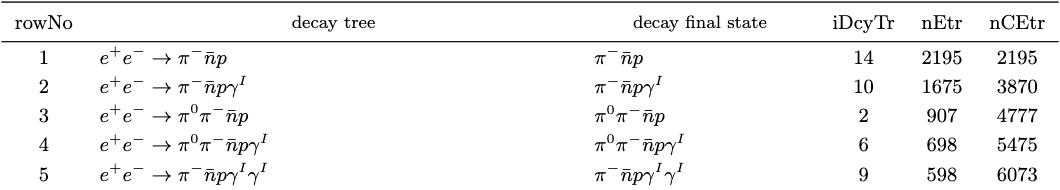
\includegraphics[width=1\textwidth]{nbar_cocktail/images/topo_uubar_010}
    \caption{Top 5 channels from the TopoAna output for the $u\bar{u}$ Monte Carlo cocktail. NO ISR case.}
    \label{fig:topo_nog_010_uubar}
\end{figure}

After applying the $\alpha < 0.10$ rad cut, the dominant contribution remains from the signal channel $p \pi^- \bar{n}$, now immediately followed by $p \pi^- \bar{n} \gamma_{\text{ISR}}$. Both contributions can be identified as signal since they fall within the signal region $[0.8,1.2]$ GeV.

\subsection{$q\bar{q}$ cocktail production (NO ISR case)}
In order to fully characterize the Monte Carlo simulation, all $q\bar{q}$ continuum components are studied. The Run 1 Monte Carlo productions for $u\bar{u}$, $d\bar{d}$, $s\bar{s}$, and $c\bar{c}$ are therefore analyzed.
$\\$
For a cleaner comparison between the signal channel and background components, the TopoAna output can be consulted in Fig.~\ref{fig:topo_nog_010_qqbar}.
\begin{figure}[H]
    \centering
    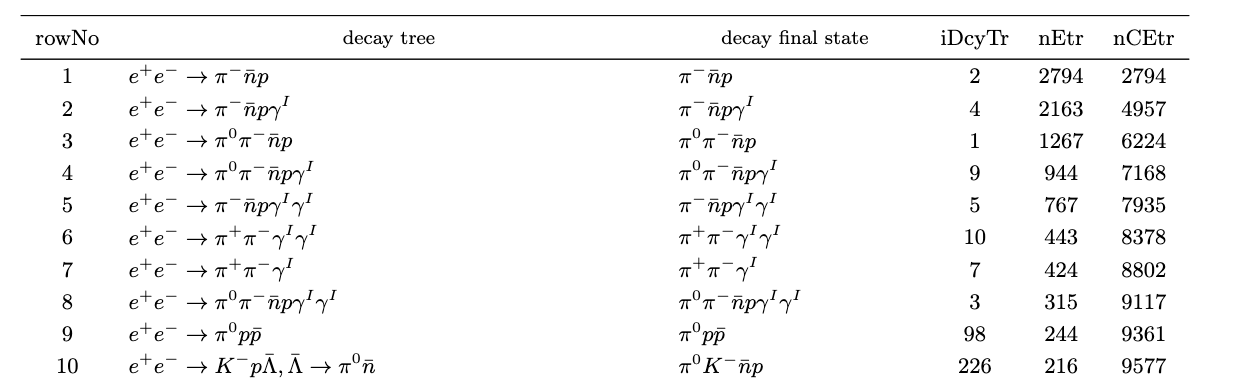
\includegraphics[width=1\textwidth]{nbar_cocktail/images/topoana_nog_010_qqbar}
    \caption{First 10 channels of the TopoAna output in $q\bar{q}$ Monte Carlo cocktail, showing the different channel contributes.}
    \label{fig:topo_nog_010_qqbar}
\end{figure}
The TopoAna output reveals that the dominant contribution is from the signal channel $p \pi^- \bar{n}$ in the $q\bar{q}$ continuum. A secondary contribution comes from $p \pi^- \bar{n} \gamma_{ISR}$, which could be treated as signal despite the $\gamma_{\text{ISR}}$ not being explicitly reconstructed. The next contribution comes from $p \pi^- \bar{n} \pi^0$ in the final state. The fourth contribution is due to $p \pi^- \bar{n} \pi^0 \gamma_{\text{ISR}}$, and so on. The situation is very similar to that observed in the $u\bar{u}$ case.
$\\$
The individual TopoAna outputs separately for the $u\bar{u}$, $d\bar{d}$, $s\bar{s}$, and $c\bar{c}$ samples are now discussed. The first 5 contributes for each sample are shown in ~\ref{fig:topo_nog_010_qqbar_singles}.
\begin{figure}[h]
    \centering
    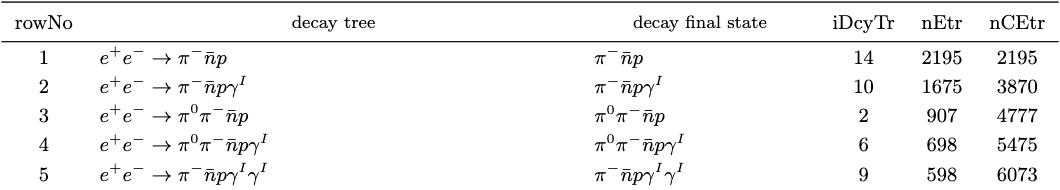
\includegraphics[width=1\textwidth]{nbar_cocktail/images/topo_uubar_010}
    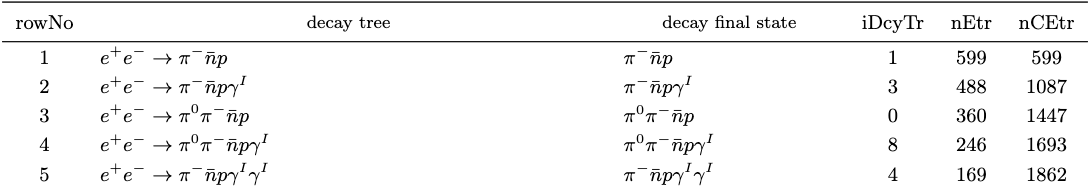
\includegraphics[width=1\textwidth]{nbar_cocktail/images/topo_ddbar_010}
    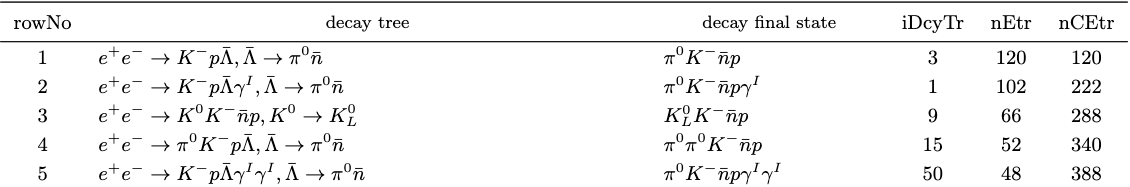
\includegraphics[width=1\textwidth]{nbar_cocktail/images/topo_ssbar_010}
    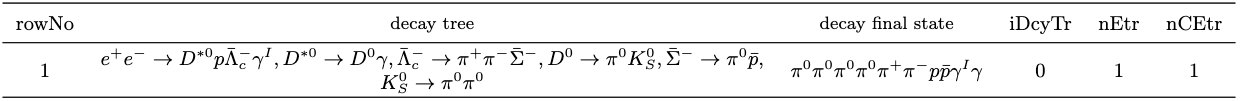
\includegraphics[width=1\textwidth]{nbar_cocktail/images/topo_ccbar_010}
    \caption{Top 5 channels from the TopoAna output respectively for the $u\bar{u}$, $d\bar{d}$, $s\bar{s}$, and $c\bar{c}$ Monte Carlo cocktails (from top to bottom). NO ISR case. The \texttt{iDcyTr} index values may differ across samples, since each TopoAna output is produced independently from its corresponding ROOT ntuples.}
    \label{fig:topo_nog_010_qqbar_singles}
\end{figure}
The main contributions to the final signal state are from the $u\bar{u}$ and $d\bar{d}$ cocktails, as expected, since no $p\pi^-\bar{n}$ system can be obtained from an $s\bar{s}$ state. A contribution from a $c\bar{c}$ state could have been expected from the following channel:

\begin{center}
$e- \ + \ e^- \rightarrow J/\Psi (c\bar{c}) \rightarrow p \ + \ \pi^- \ + \ \bar{n}$
\end{center}
In order to reach the $J/\psi$ resonance ($\sim 3.1$ GeV) in $e^+e^-$ collisions at Belle II, a significant lowering of the center-of-mass energy must occur due to $\gamma_{\rm ISR}$ emission. Since high-energy ISR emission is improbable (Fig.~\ref{fig:isr_distro}), the $c\bar{c}$ channel can be considered negligible for this analysis.
$\\$
The obtained stacked components to the recoil mass, in $q\bar{q}$ cocktail, are shown in figure ~\ref{fig:mRecComps_nog_010_qqbar}.
\begin{figure}[H]
    \centering
    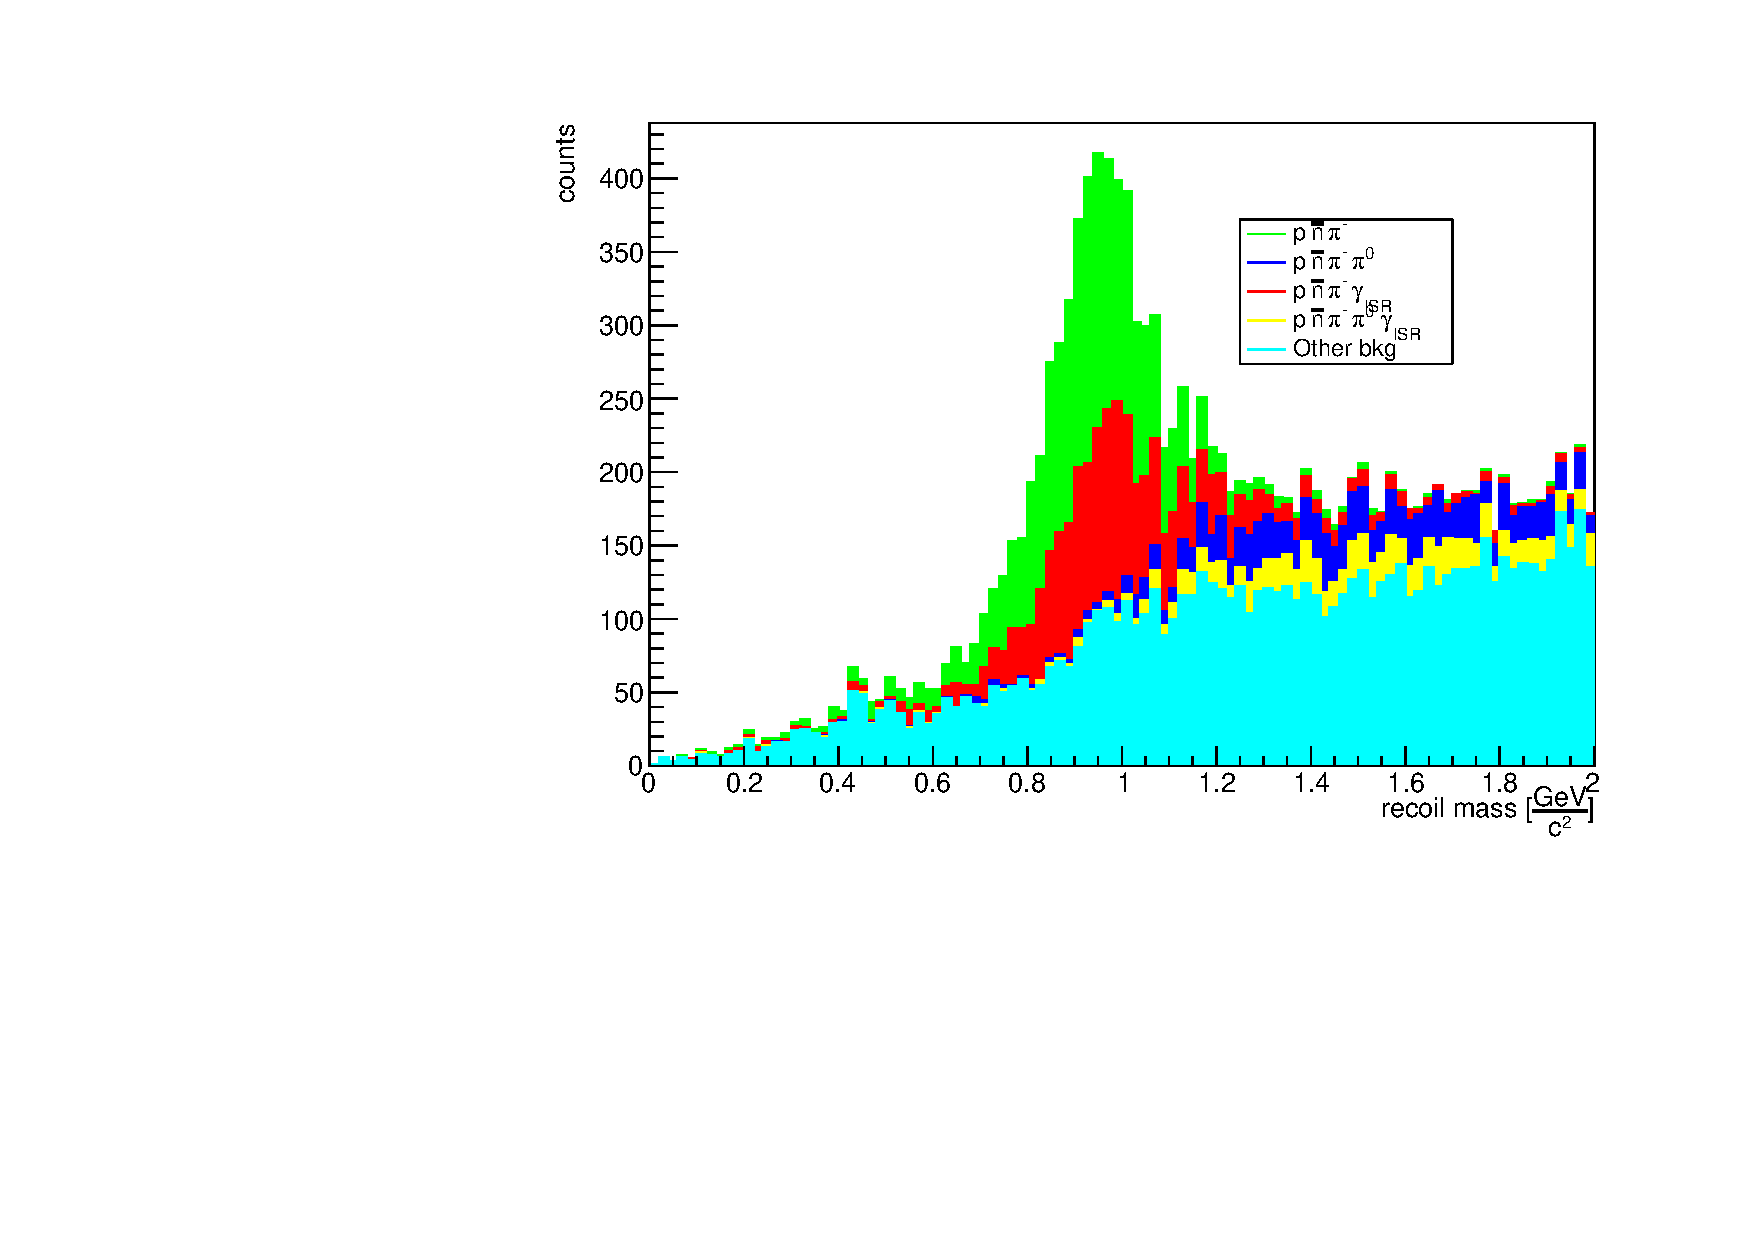
\includegraphics[width=0.8\textwidth]{nbar_cocktail/images/recoilM_qqbar_comps_nog_010}
    \caption{$p, \pi^-$ recoil mass distribution in $q\bar{q}$ Monte Carlo cocktail, displaying each stacked component contribution, NO ISR case. Green: $\pi^- \bar{n} p$ channel. Blue: $\pi^0 \pi^- \bar{n} p$ channel. Red: $\pi^- \bar{n} p \gamma_{ISR}$. Yellow: $\pi^0 \pi^- \bar{n} p \gamma_{ISR}$ channel. Cyan: other channels. $\alpha<$ 10 rad cut is applied.}
    \label{fig:mRecComps_nog_010_qqbar}
\end{figure}
A similar behaviour to the $u\bar{u}$ cocktail can be observed, where the $p\pi^-\bar{n}$ and $p\pi^-\bar{n}\gamma_{\text{ISR}}$ channels mainly contribute to the signal region [0.8,1.2] GeV. Background components containing the $\pi^0$ peak appear outside the signal region [0.8,1.2] GeV on the right side, while a flat background is present from other background channels.

\subsubsection{Cluster variables in $q\bar{q}$ cocktail}
The $\bar{n}$ candidates reconstructed cluster variables can now be studied with the following discussed selections:
\begin{enumerate}
\item Recoil system: $0 \ GeV/c^2 <recoil \ mass < 2 \ GeV/c^2$ and in ECL acceptance;
\item $\bar{n}$: neutral clusters from ECL and number of hits $> 10$ and energy $<3$ GeV;
\item $p$: $protonID > 0.9$ and $dr<1$ cm and $|dz|<3$ cm;
\item $\pi^-$: $pionID > 0.1$ and $dr<1$ cm and $|dz|<3$ cm; 
\item $\alpha <0.10$ rad $\sim 5.73^\circ$;
\item No further charged particles in the Rest of Event (ROE).
\end{enumerate}
The obtained $\bar{n}$ candidates reconstructed cluster variables are shown in Fig.\ref{fig:clus_vars_nog_qqbar}.
Specific structures can be observed in the cluster variables distributions, compared to those obtained in Fig.~\ref{fig:clus_vars_2}.
$\\$
For example, in the E1E9 distribution a second structure can be noted at a value $\sim 0.85$, and at value $\sim 1$ in the E9E21distribution as well. Similar structure appears at values close to 0 in the Second Moment distribuiton, which is partially reflected in the first structure of the N Hits distribution observed at a value of $\sim 10$. Another example can be seen in the Lateral Momentum distribution, where a structure at $\sim 0.3$ can be noted, which is typical reference of electromagnetic shower. 
$\\$
Therefore, a contribution from small-sized clusters -as can be seen in the Second Moment and N Hits distributions- and not spread out clusters -as can be seen in the E1E9 and E9E21 distributions- can be observed in $\bar{n}$ candidates reconstructed cluster variables. These shower shape characteristics are typical of the electromagnetic showers. This is further suggested by the structure observed in the Lateral Momentum distribution.
$\\$
In order to study the nature of these singular structures, a signal and background study can be performed, isolating the individual contribution of each. If these structures are not produced by the signal, their contribution could be isolated and then removed from the signal one. In order to perform this kind of analysis, the sidebands technique is discussed in the next paragraph.

\newpage
The obtained cluster variables distribution in NO ISR case, in q$\bar{q}$ cocktail.
 \begin{figure}[H]
    \centering
    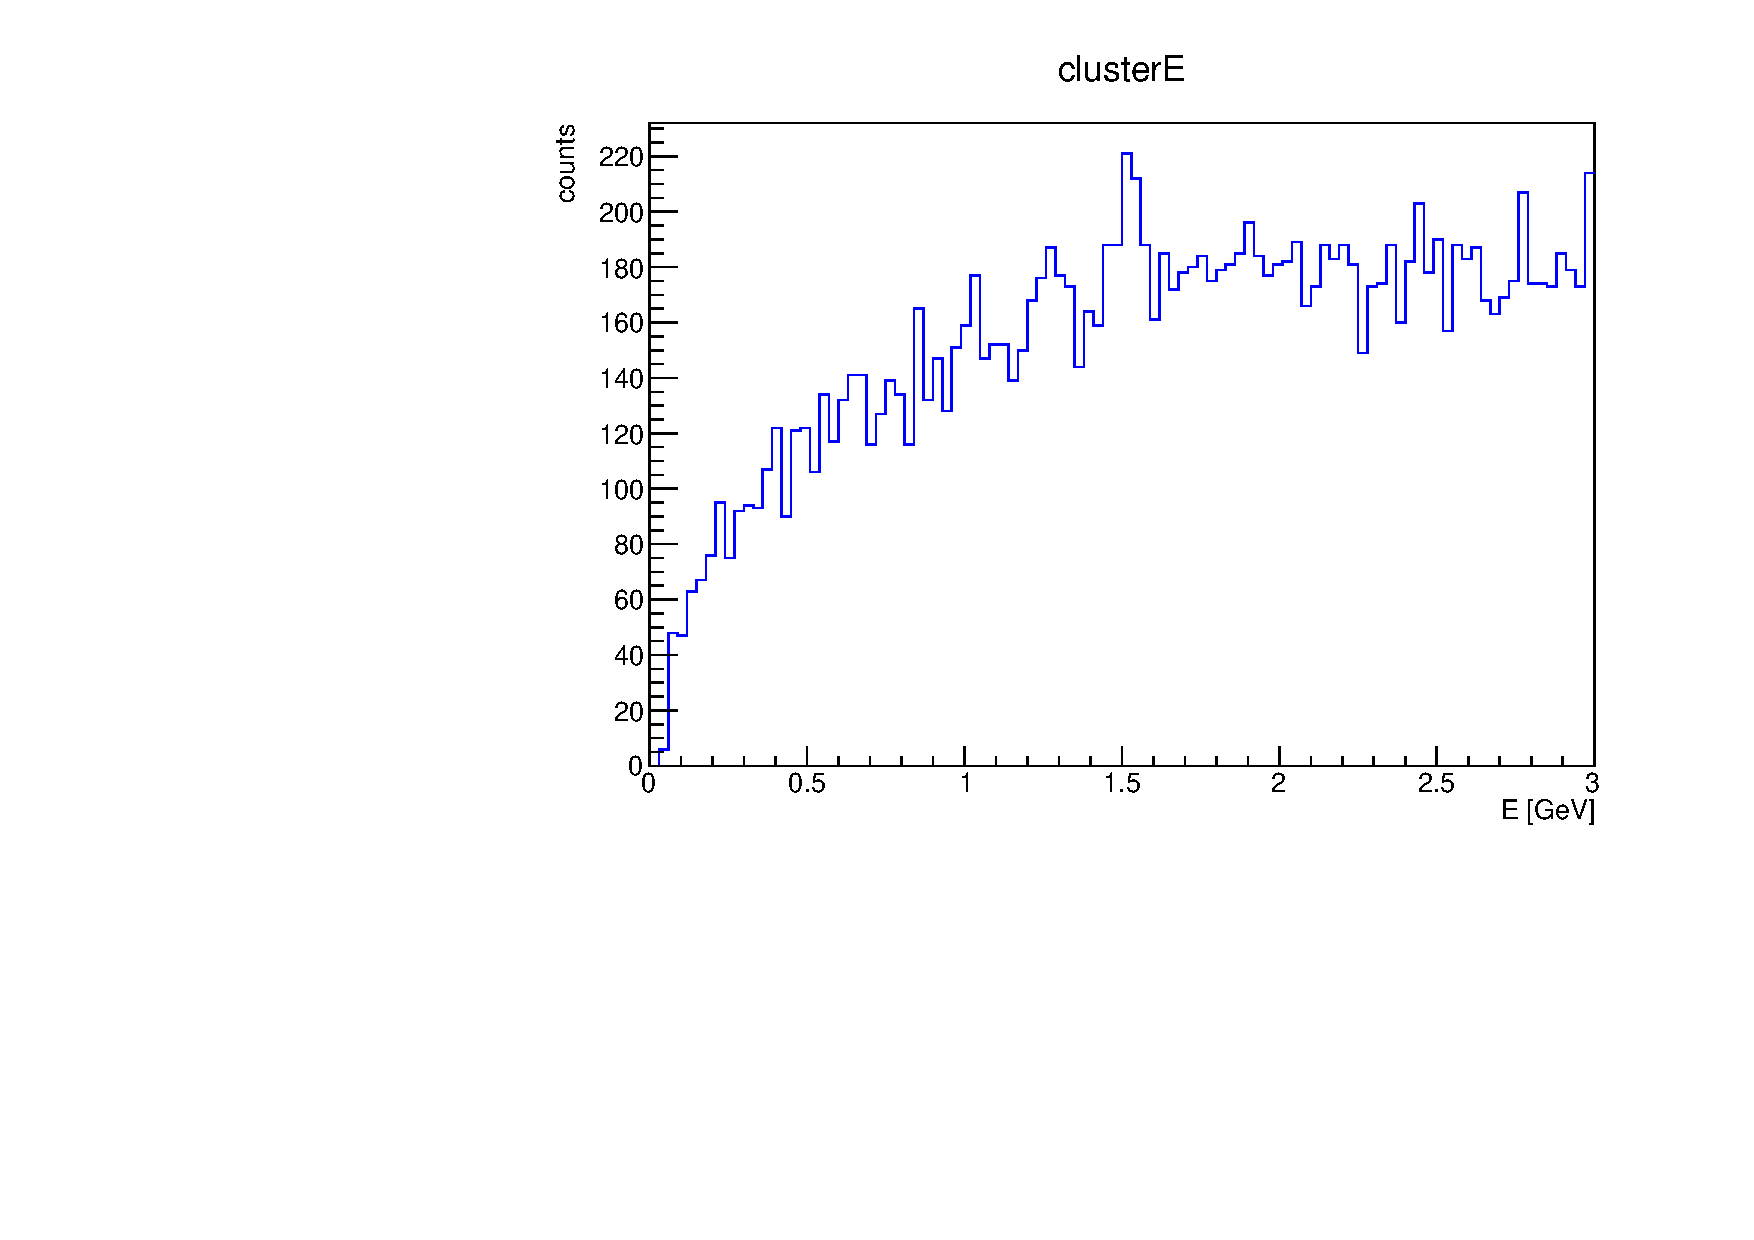
\includegraphics[width=0.49\textwidth]{nbar_cocktail/images/clusterE_nog_qqbar.pdf}
    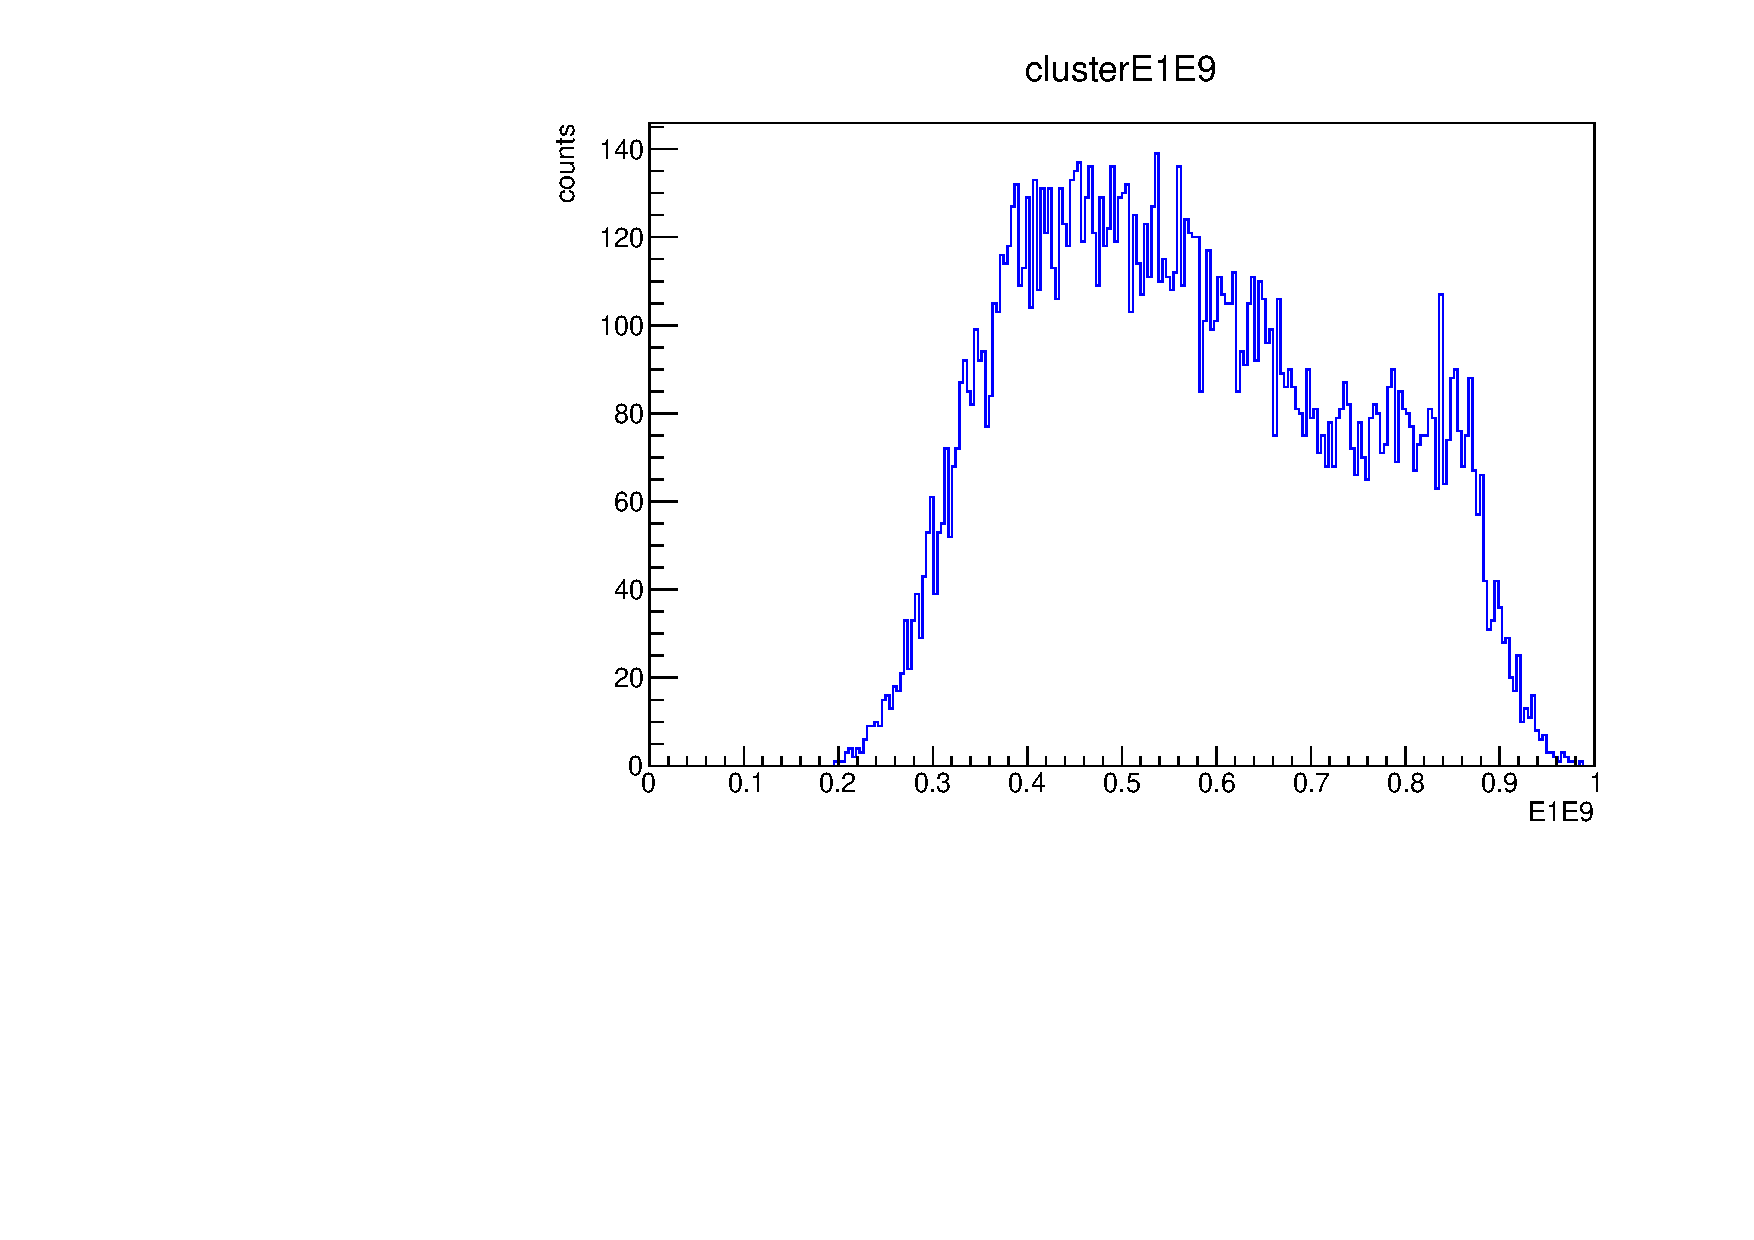
\includegraphics[width=0.49\textwidth]{nbar_cocktail/images/clusterE1E9_nog_qqbar.pdf}
    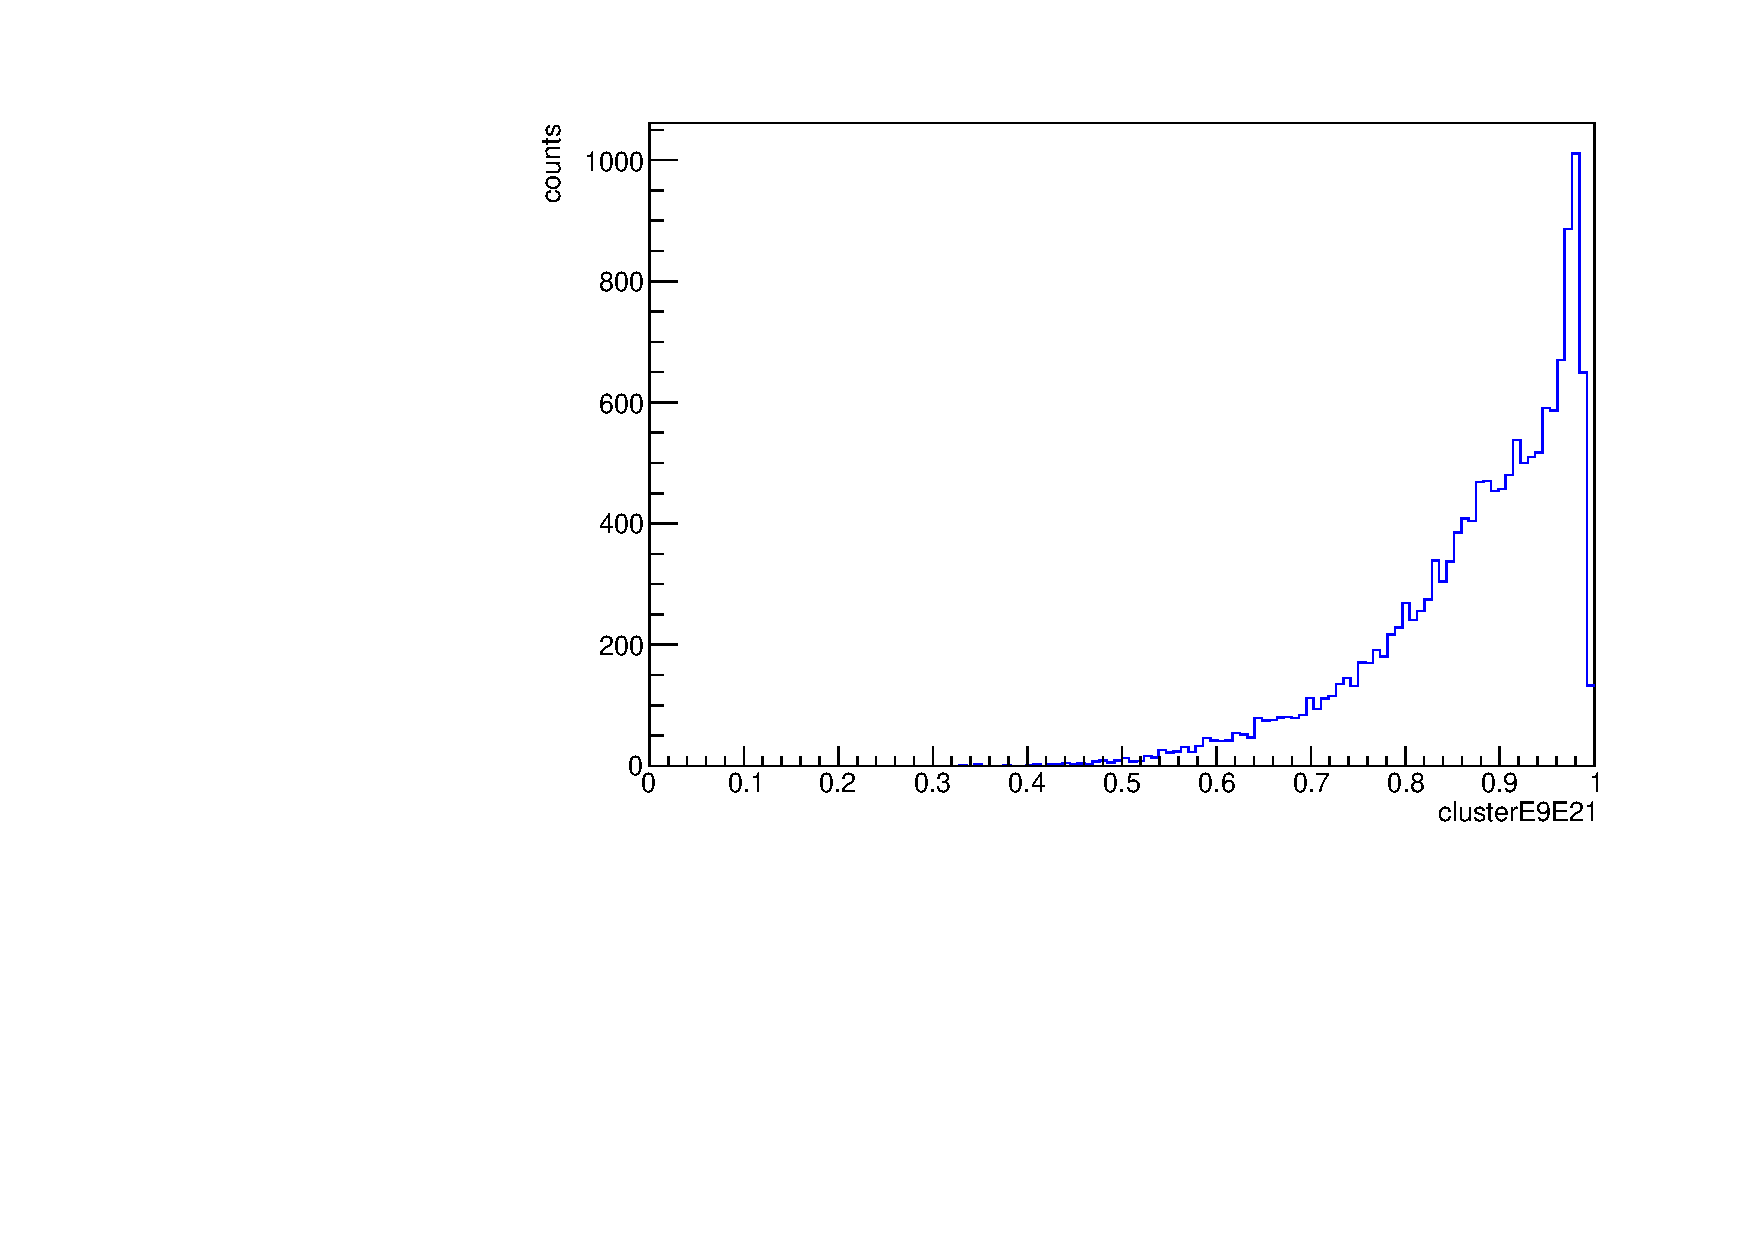
\includegraphics[width=0.49\textwidth]{nbar_cocktail/images/clusterE9E21_nog_qqbar.pdf}
    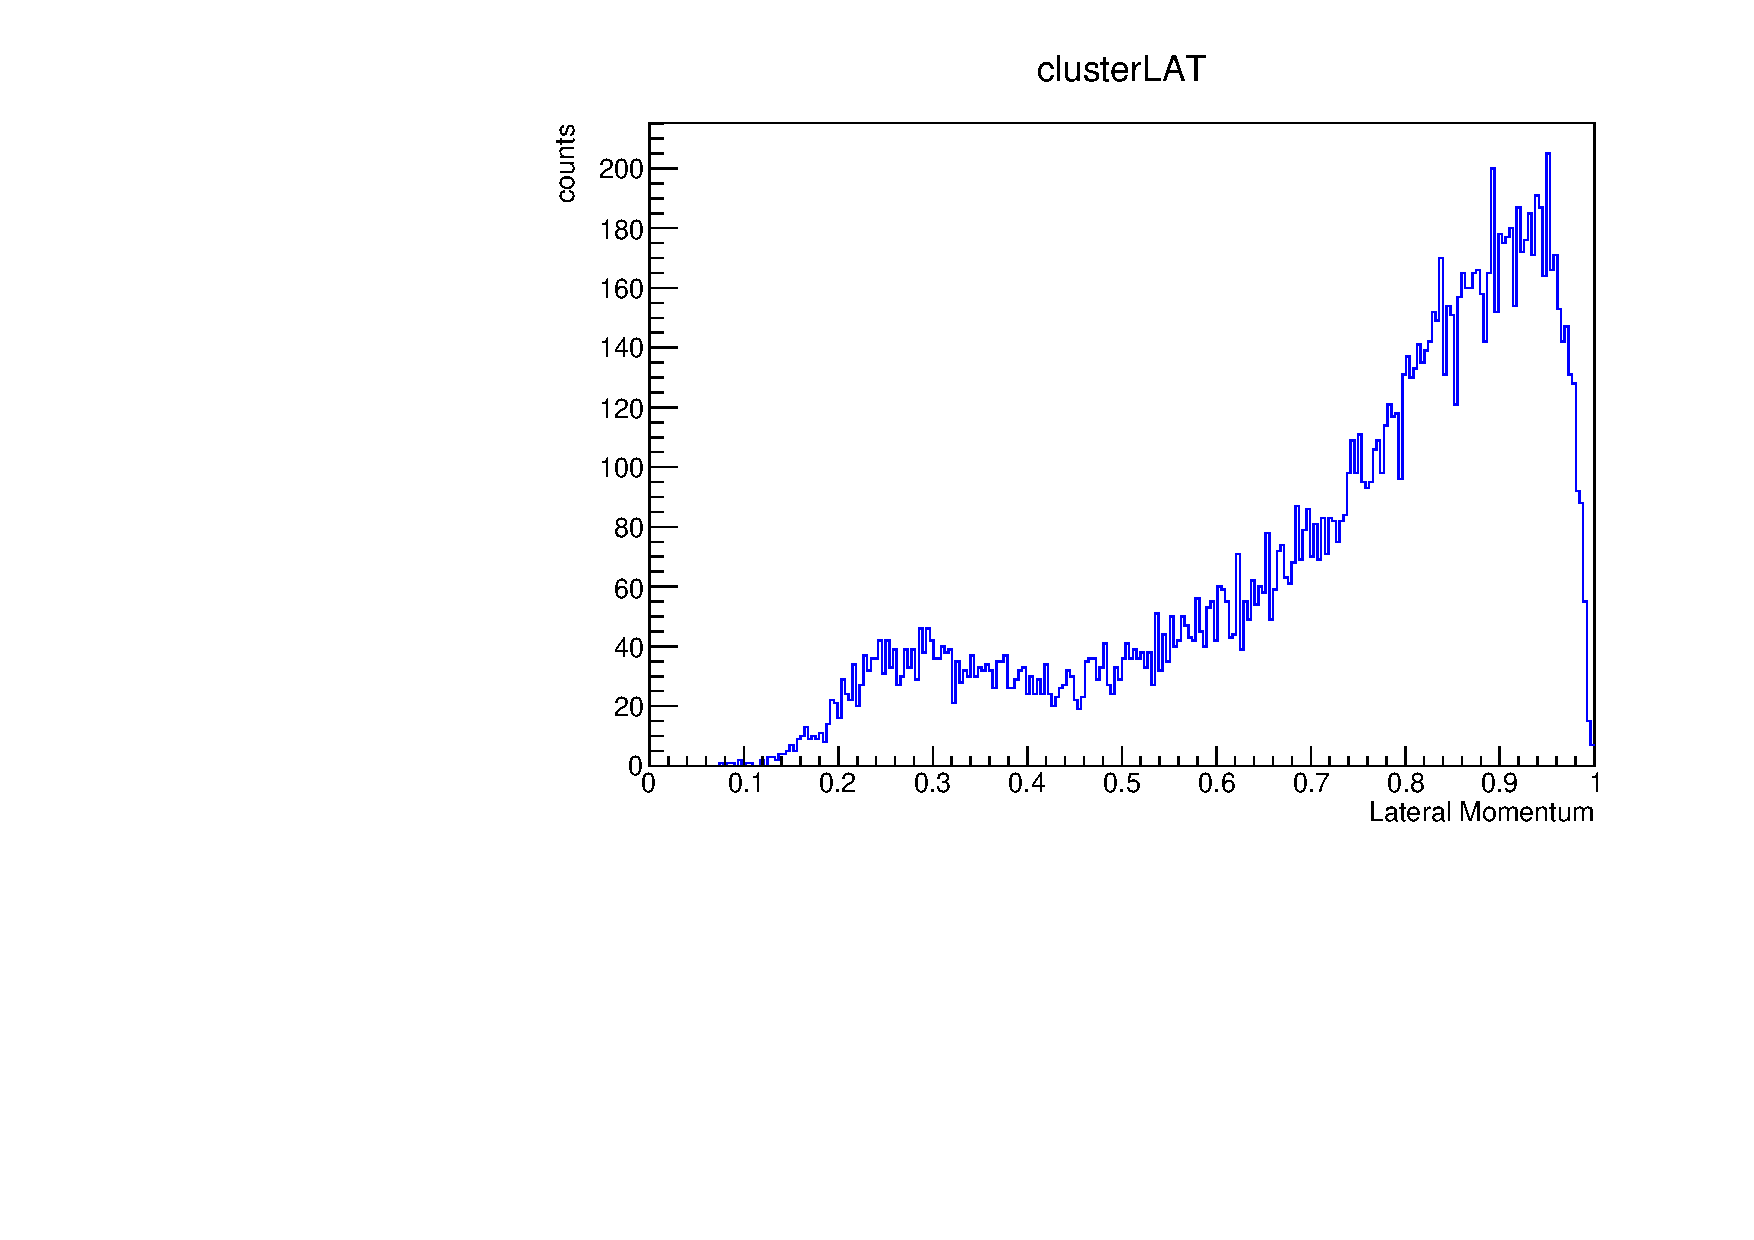
\includegraphics[width=0.49\textwidth]{nbar_cocktail/images/clusterLAT_nog_qqbar.pdf}
    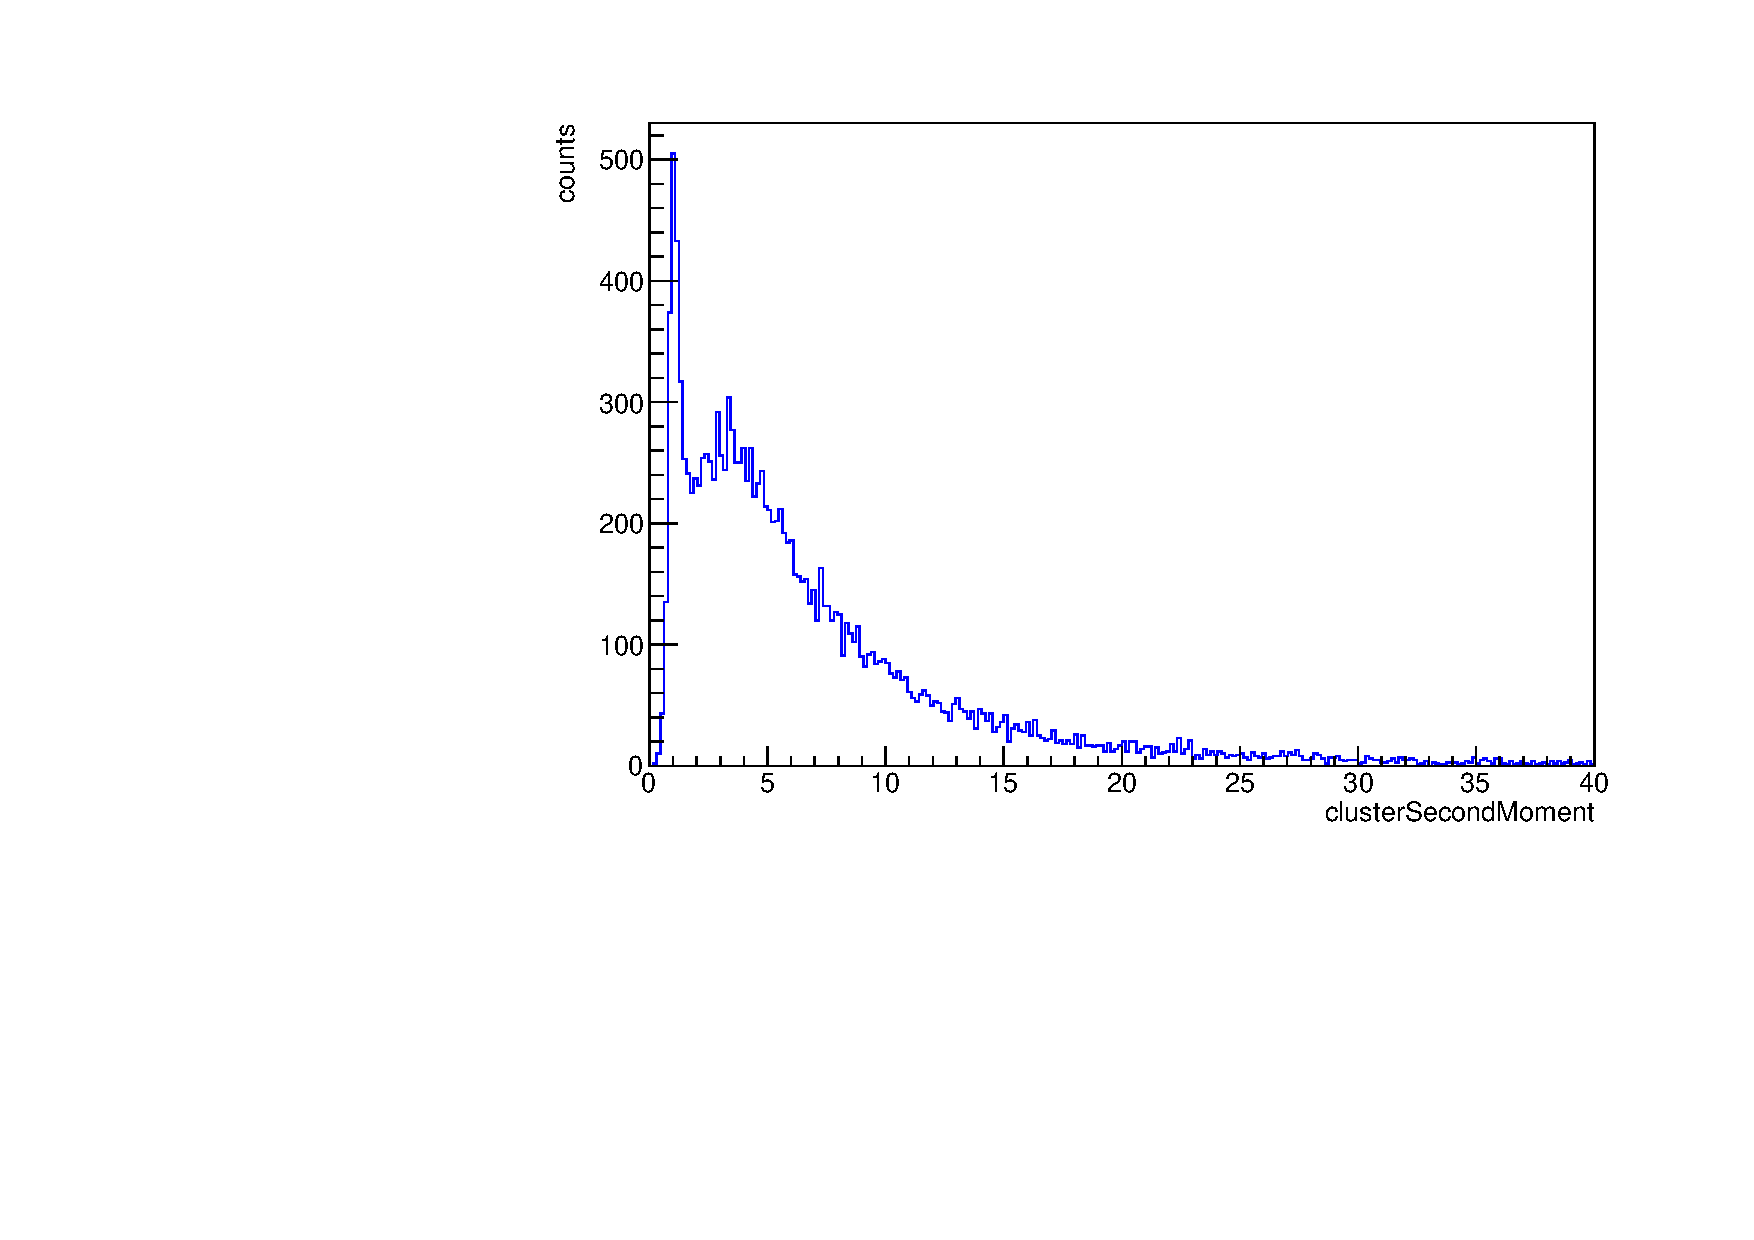
\includegraphics[width=0.49\textwidth]{nbar_cocktail/images/clusterSecondMoment_nog_qqbar.pdf}
    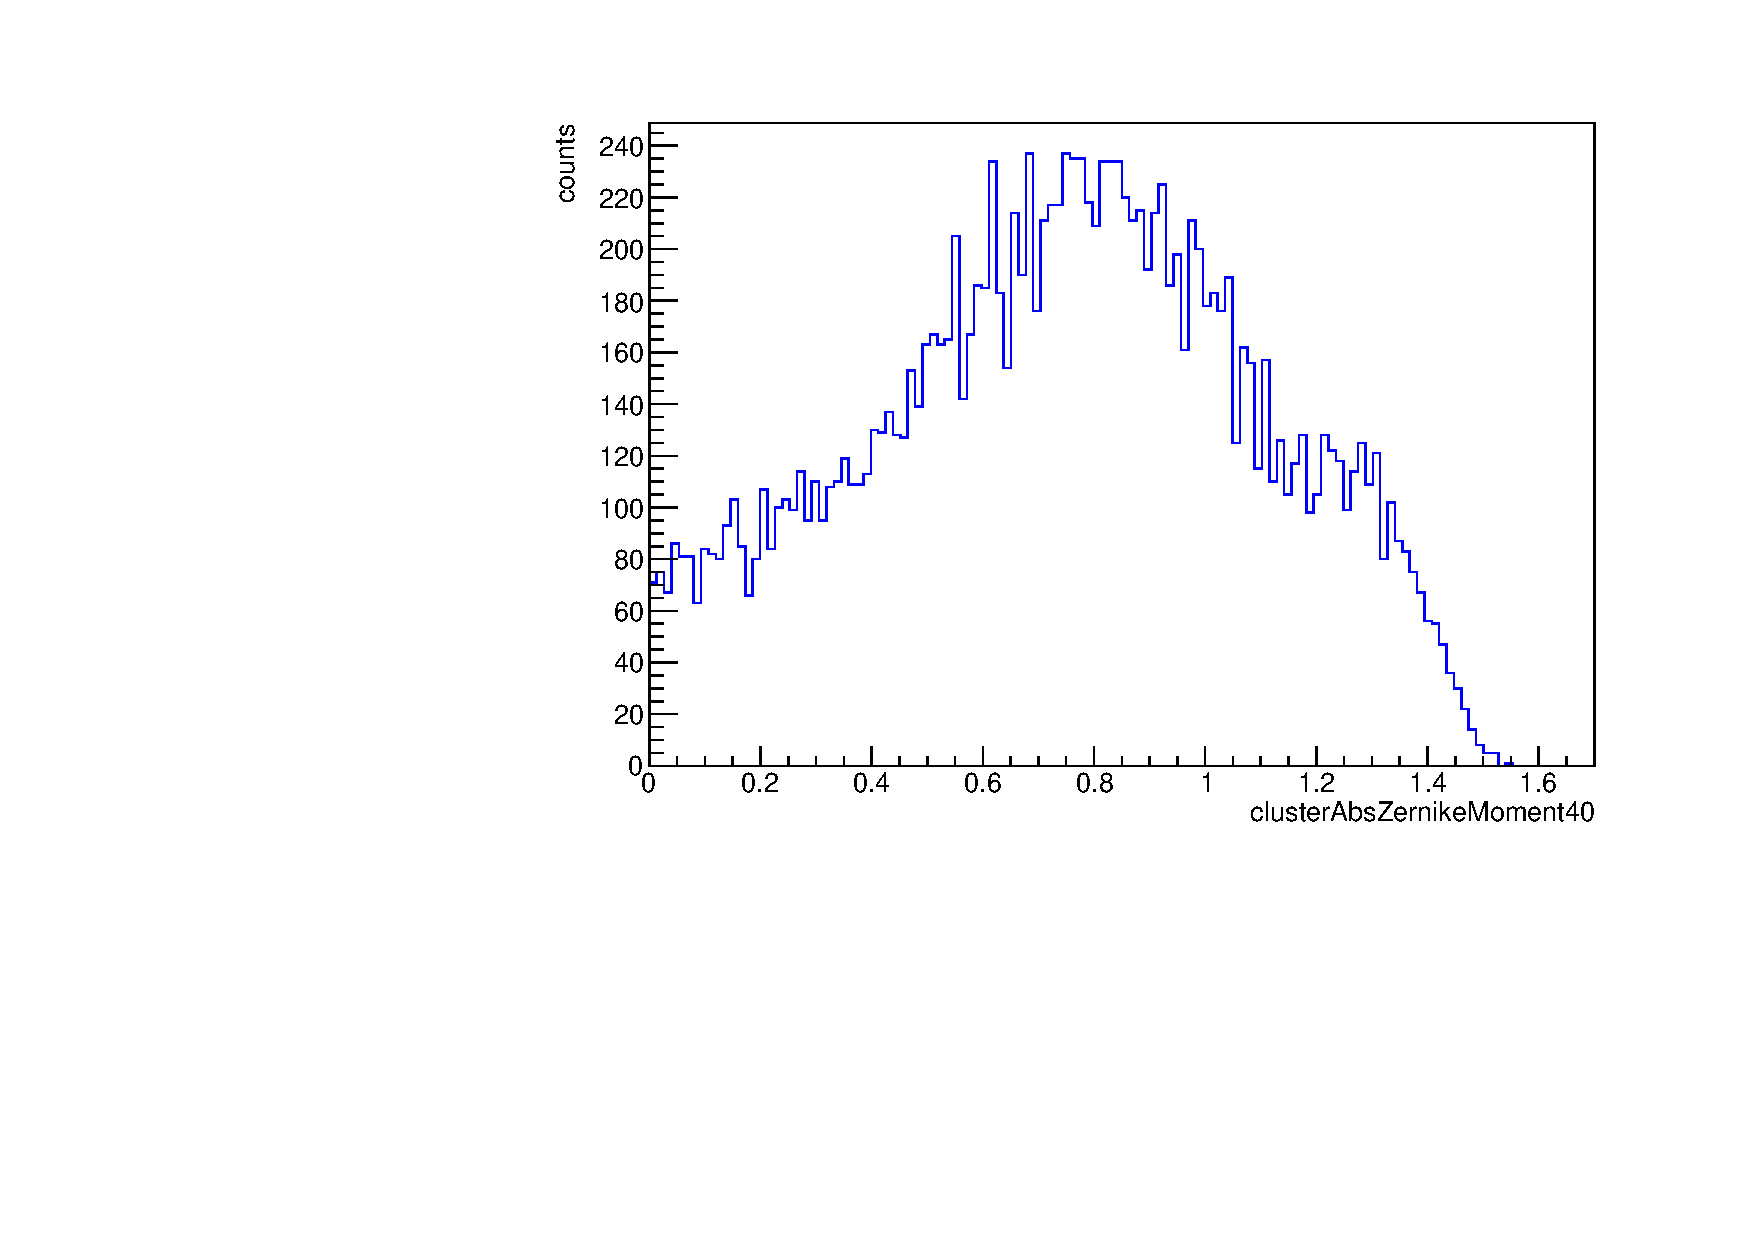
\includegraphics[width=0.49\textwidth]{nbar_cocktail/images/clusterAbsZernikeMoment40_nog_qqbar.pdf}
    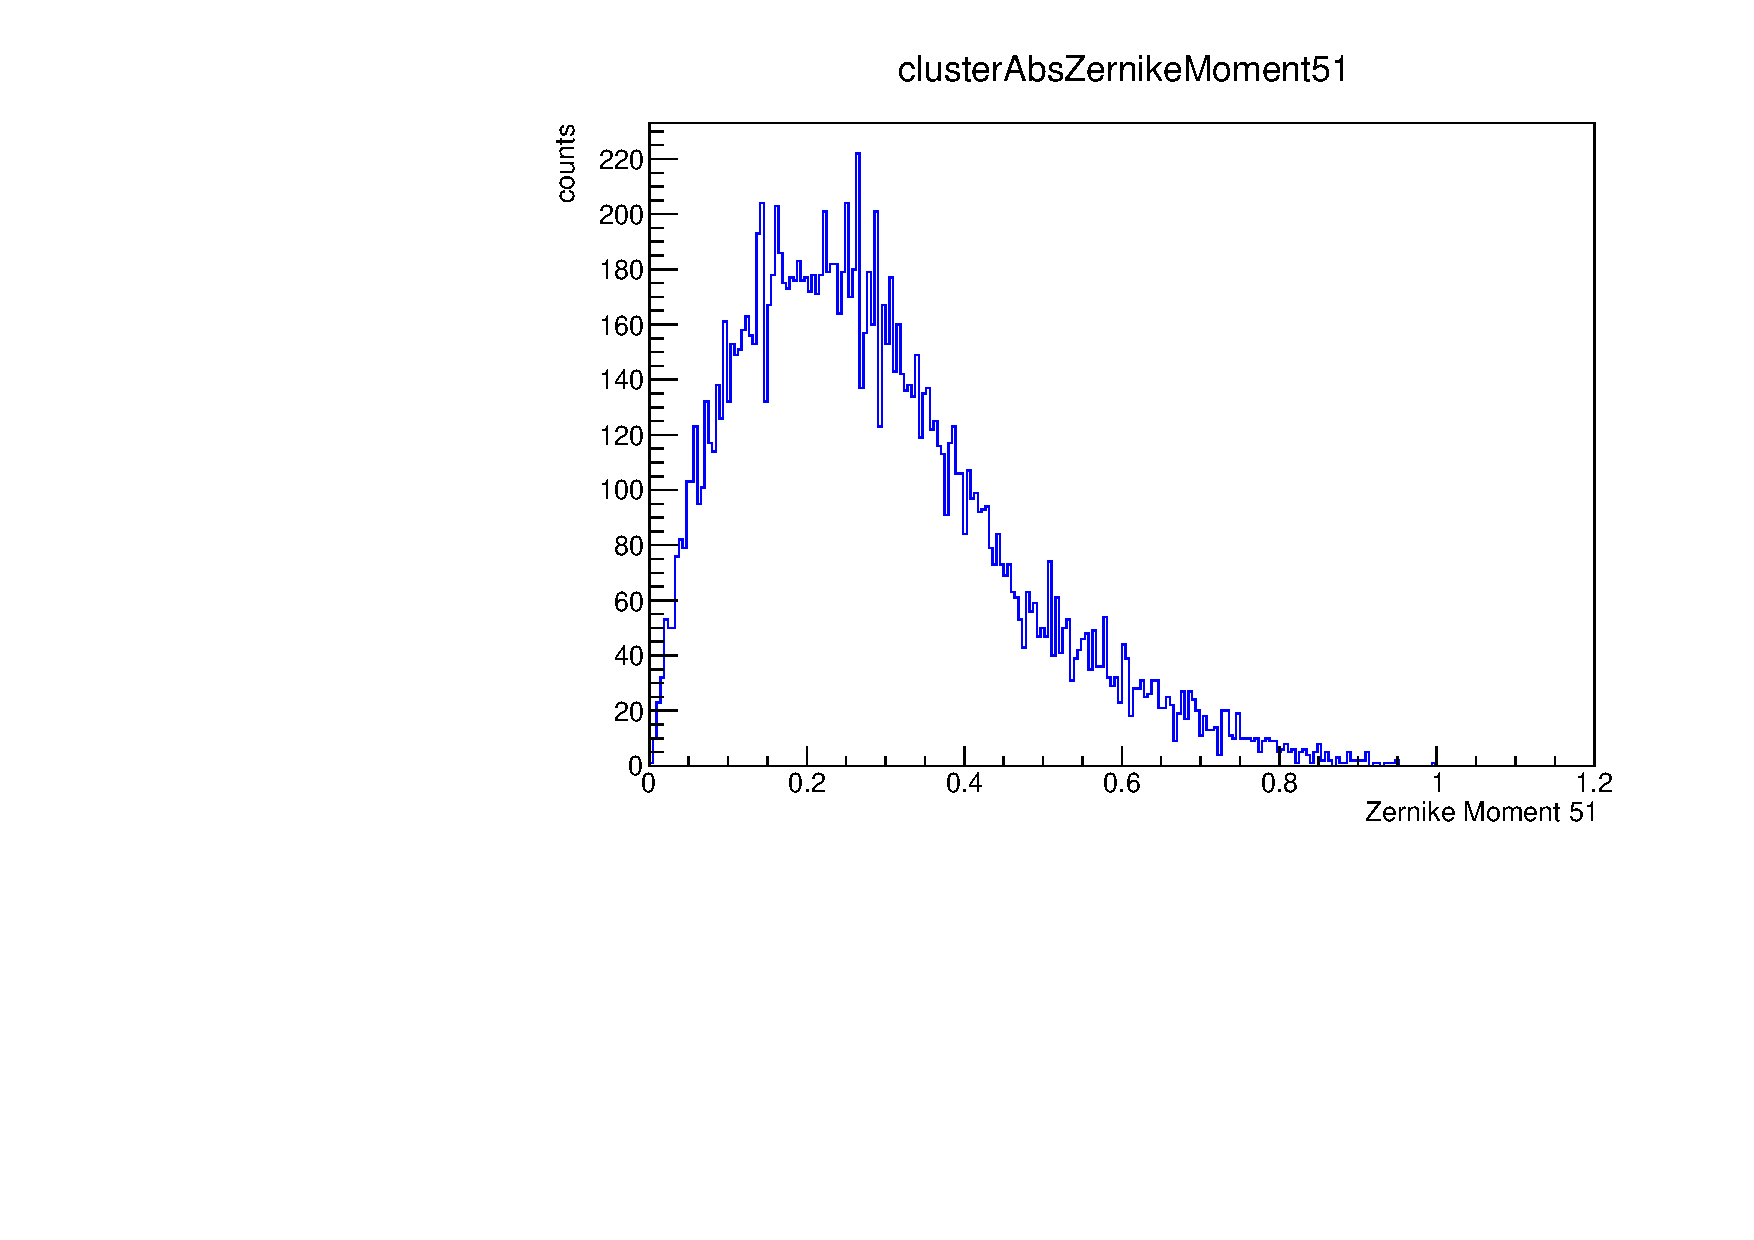
\includegraphics[width=0.49\textwidth]{nbar_cocktail/images/clusterAbsZernikeMoment51_nog_qqbar.pdf}
    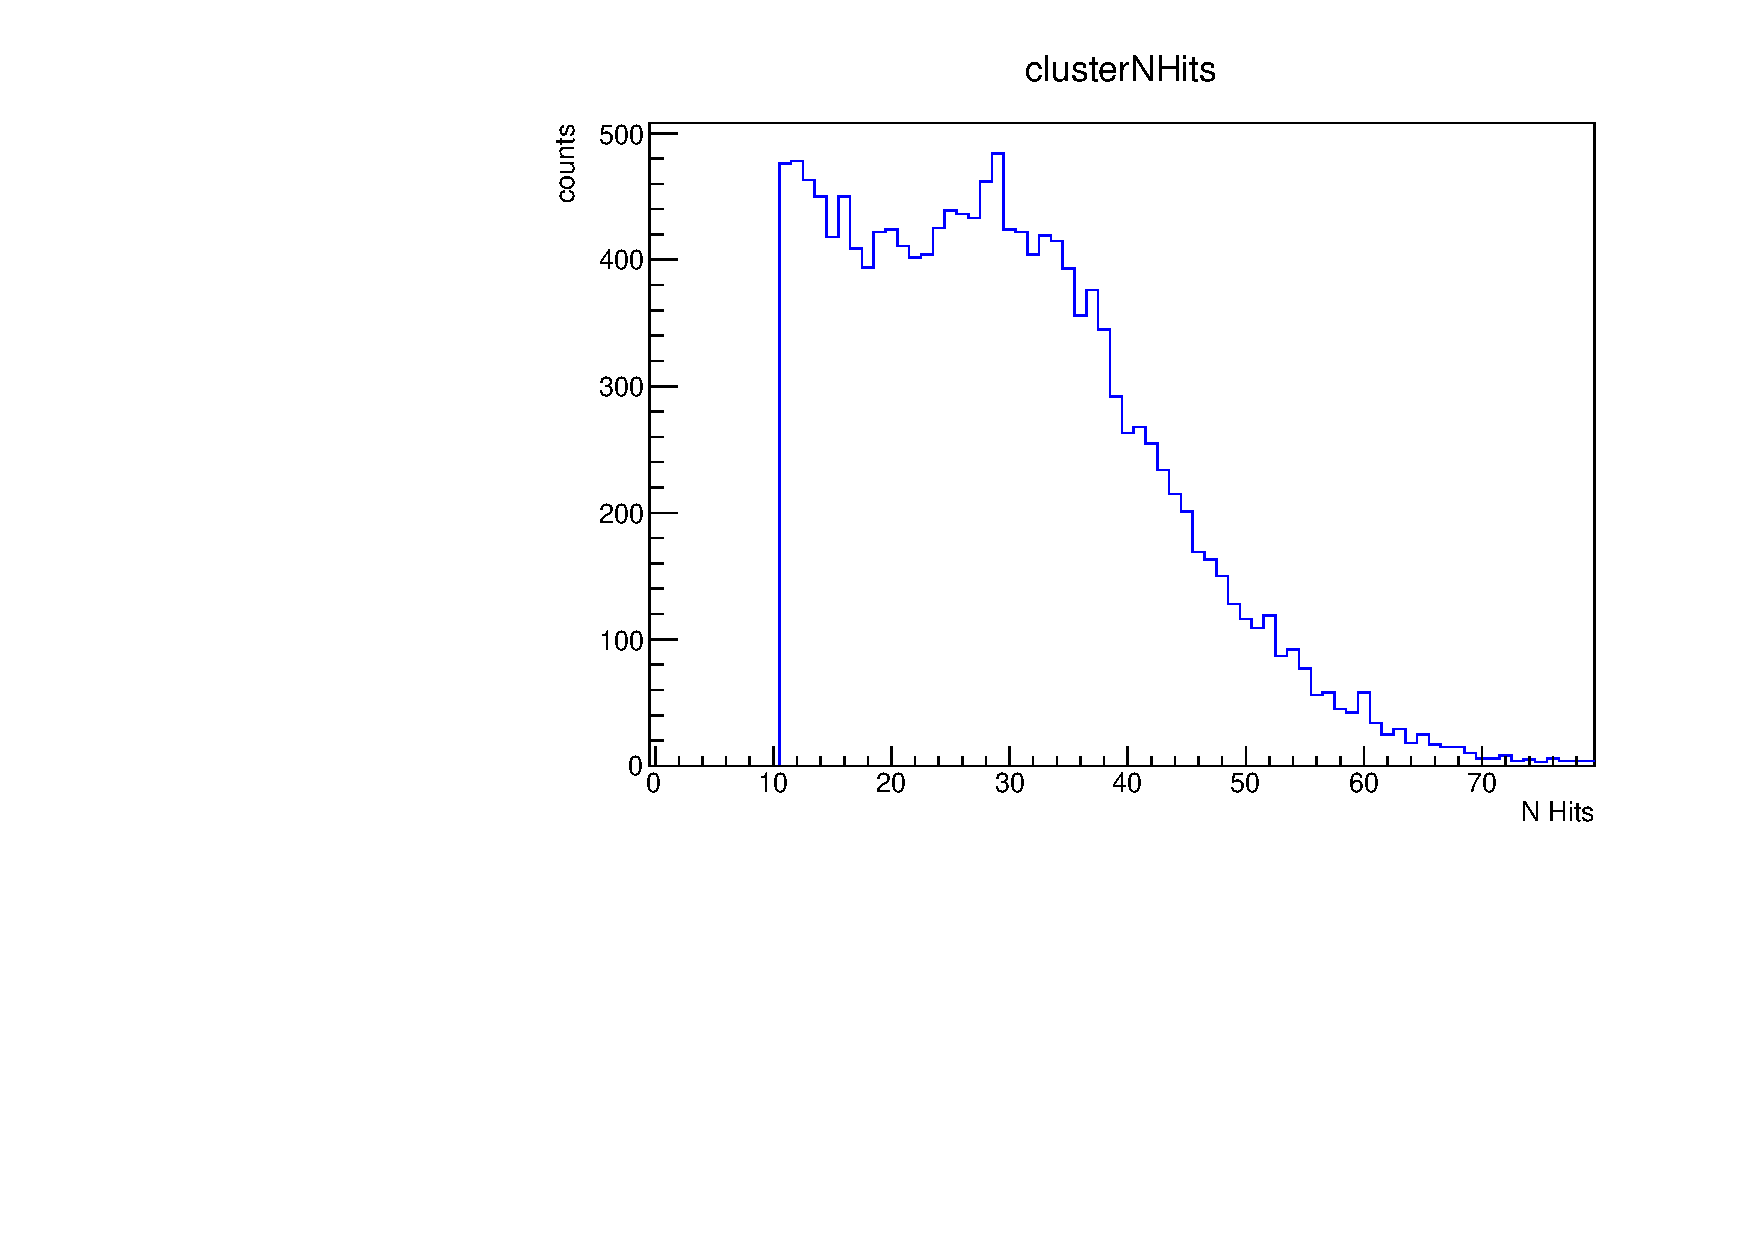
\includegraphics[width=0.49\textwidth]{nbar_cocktail/images/clusterNHits_nog_qqbar.pdf}
     \caption{Reconstructed cluster variables distribution for $\bar{n}$ candidates in the for the recoil mass region [0, 2] GeV, in NO ISR case. q$\bar{q}$ cocktail }
     \label{fig:clus_vars_nog_qqbar}
\end{figure}

\subsubsection{Sidebands technique in $q\bar{q}$ cocktail}
In order to study separately the signal and background contributions to the cluster variables, the \textbf{sidebands technique} can be adopted. 
$\\$
The sidebands technique is a data-driven method used in experimental high-energy physics to estimate and subtract the background from a region of interest. It relies on identifying a discriminating variable -often the invariant mass or the recoil mass, as this case- that separates the signal from the background. 
$\\$
The \textbf{signal region} can be defined as the region where the signal appears in the recoil mass distribution. This region contains a mixture of signal and background.
The \textbf{sidebands regions} consist of two symmetric areas (one before and one after the signal region), which may sometimes overlap, be immediately adjacent, or distant, that are assumed to contain only (or primarily) background. Therefore, in order to obtain the cluster variables distribution for the signal only, the background distribution (sidebands regions) is subtracted from the signal+background distribution (signal region) as follows:

\begin{center}
$N_{signal} = N_{\text{signal  region}} - k \cdot N_{\text{sideband region}}$,
\end{center}
where:
\begin{center}
 $k = \frac{\text{size of the signal region}}{\text{size of the sum of the sidebands regions}}$ 
 \end{center}
is a normalization factor.

$\\$
In the present case, the following region have been decided:

\begin{itemize}
\item Signal region: [0.8, 1.2] GeV;
\item Sidebands regions: [0.3, 0.7] U [1.3, 1.7]  GeV;
\item $k = \frac{1.2 - 0.8}{(0.7 - 0.3) + (1.7 - 1.3)} = \frac{1}{2}$.
\end{itemize}

The signal region and sidebands region, in the recoil mass distribution observed in Fig.~\ref{fig:mRecComps_nog_010_qqbar}, are shown in Fig.\ref{fig:recMass_sidebands}.
\begin{figure}[H]
    \centering
    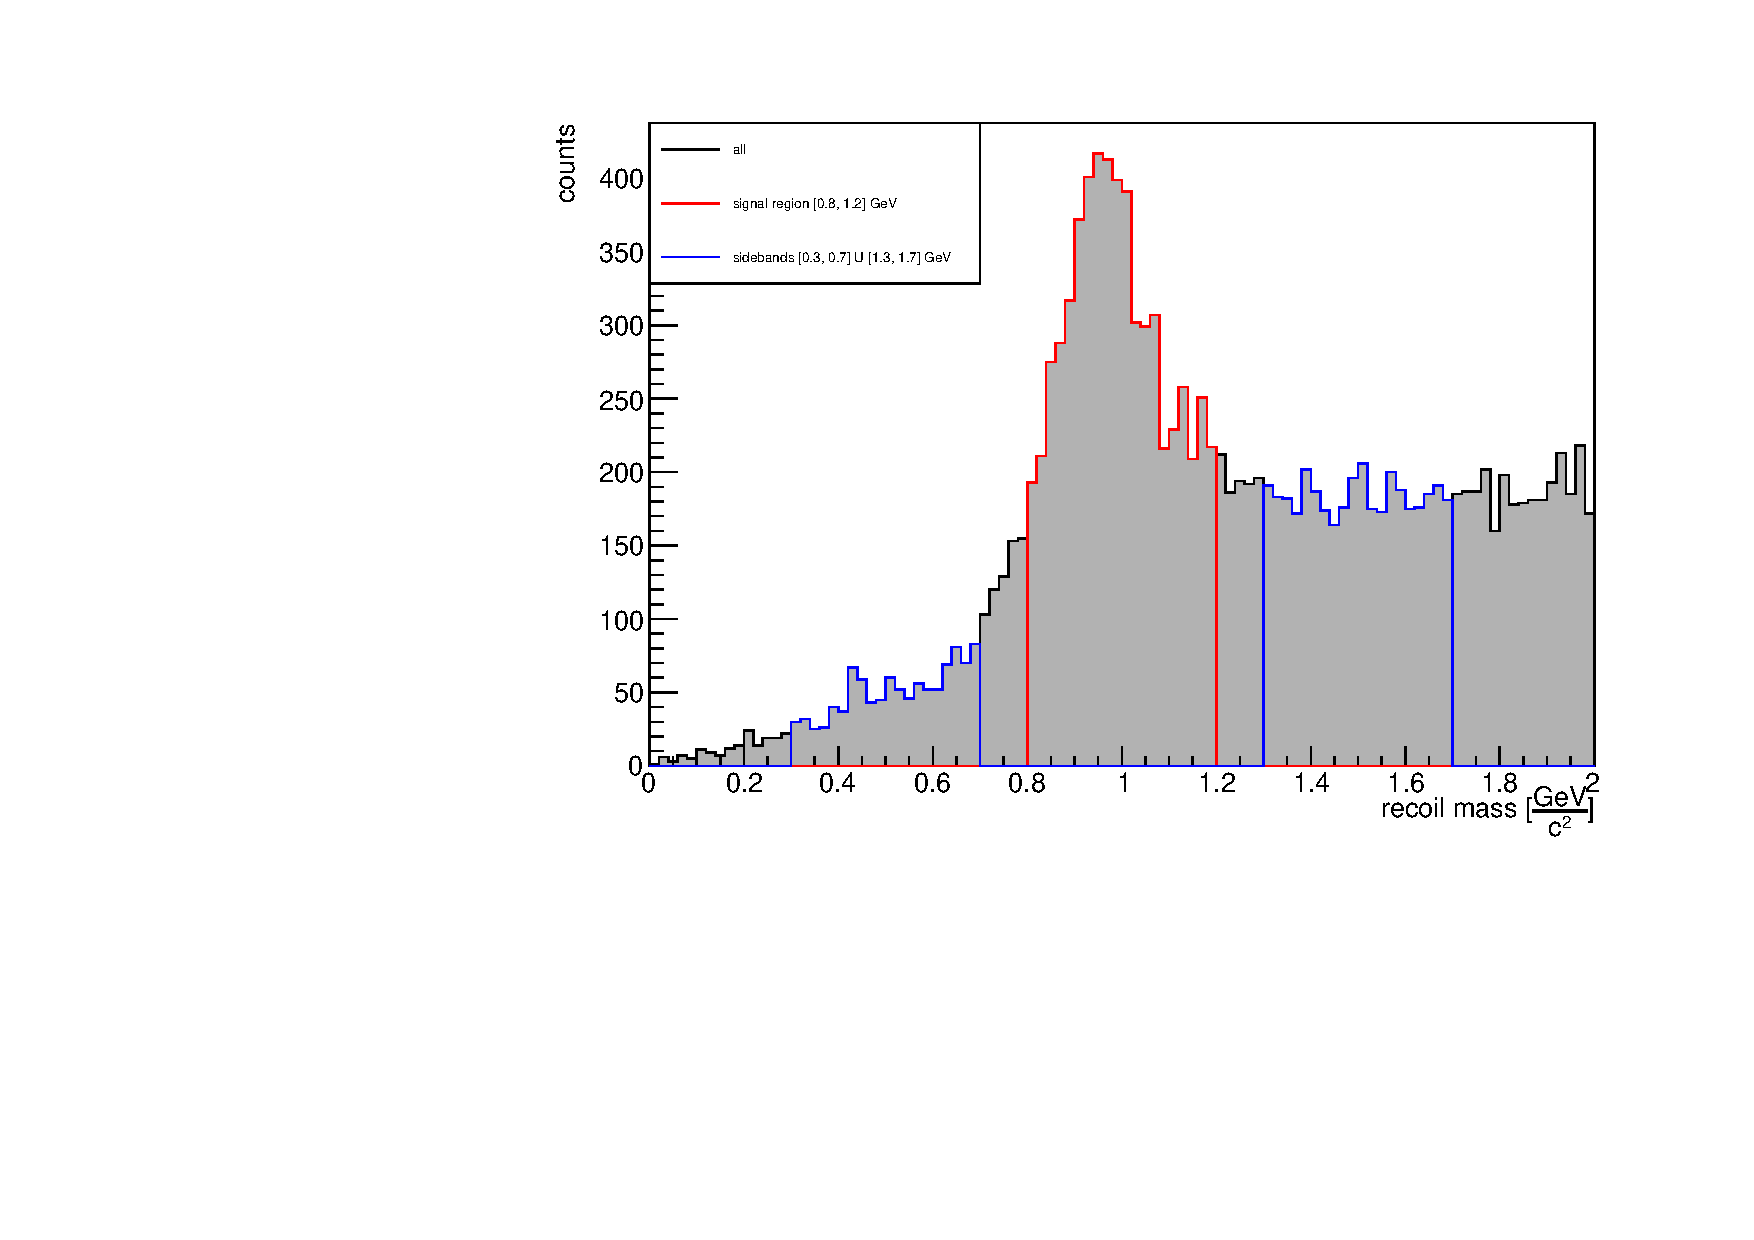
\includegraphics[width=0.6\textwidth]{nbar_cocktail/images/recoil_mass_sidebands_nog}
    \caption{Recoil mass distribution (black), with the signal region (red) and the sidebands regions (blue), in the $q\bar{q}$ Monte Carlo cocktail. NO ISR case.}
    \label{fig:recMass_sidebands}
\end{figure}
$\\$
The single contributions from the signal region and the two sidebands regions to the cluster variable can be compared. Since the two sidebands regions combined are two times larger than the signal region, a scaling factor of $k = 0.5$ has been applied to the cluster variables obtained from the sidebands regions. The obtained cluster variables contribution is shown in Fig.\ref{fig:clus_vars_sidebands_pre}.
 \begin{figure}[h]
    \centering
    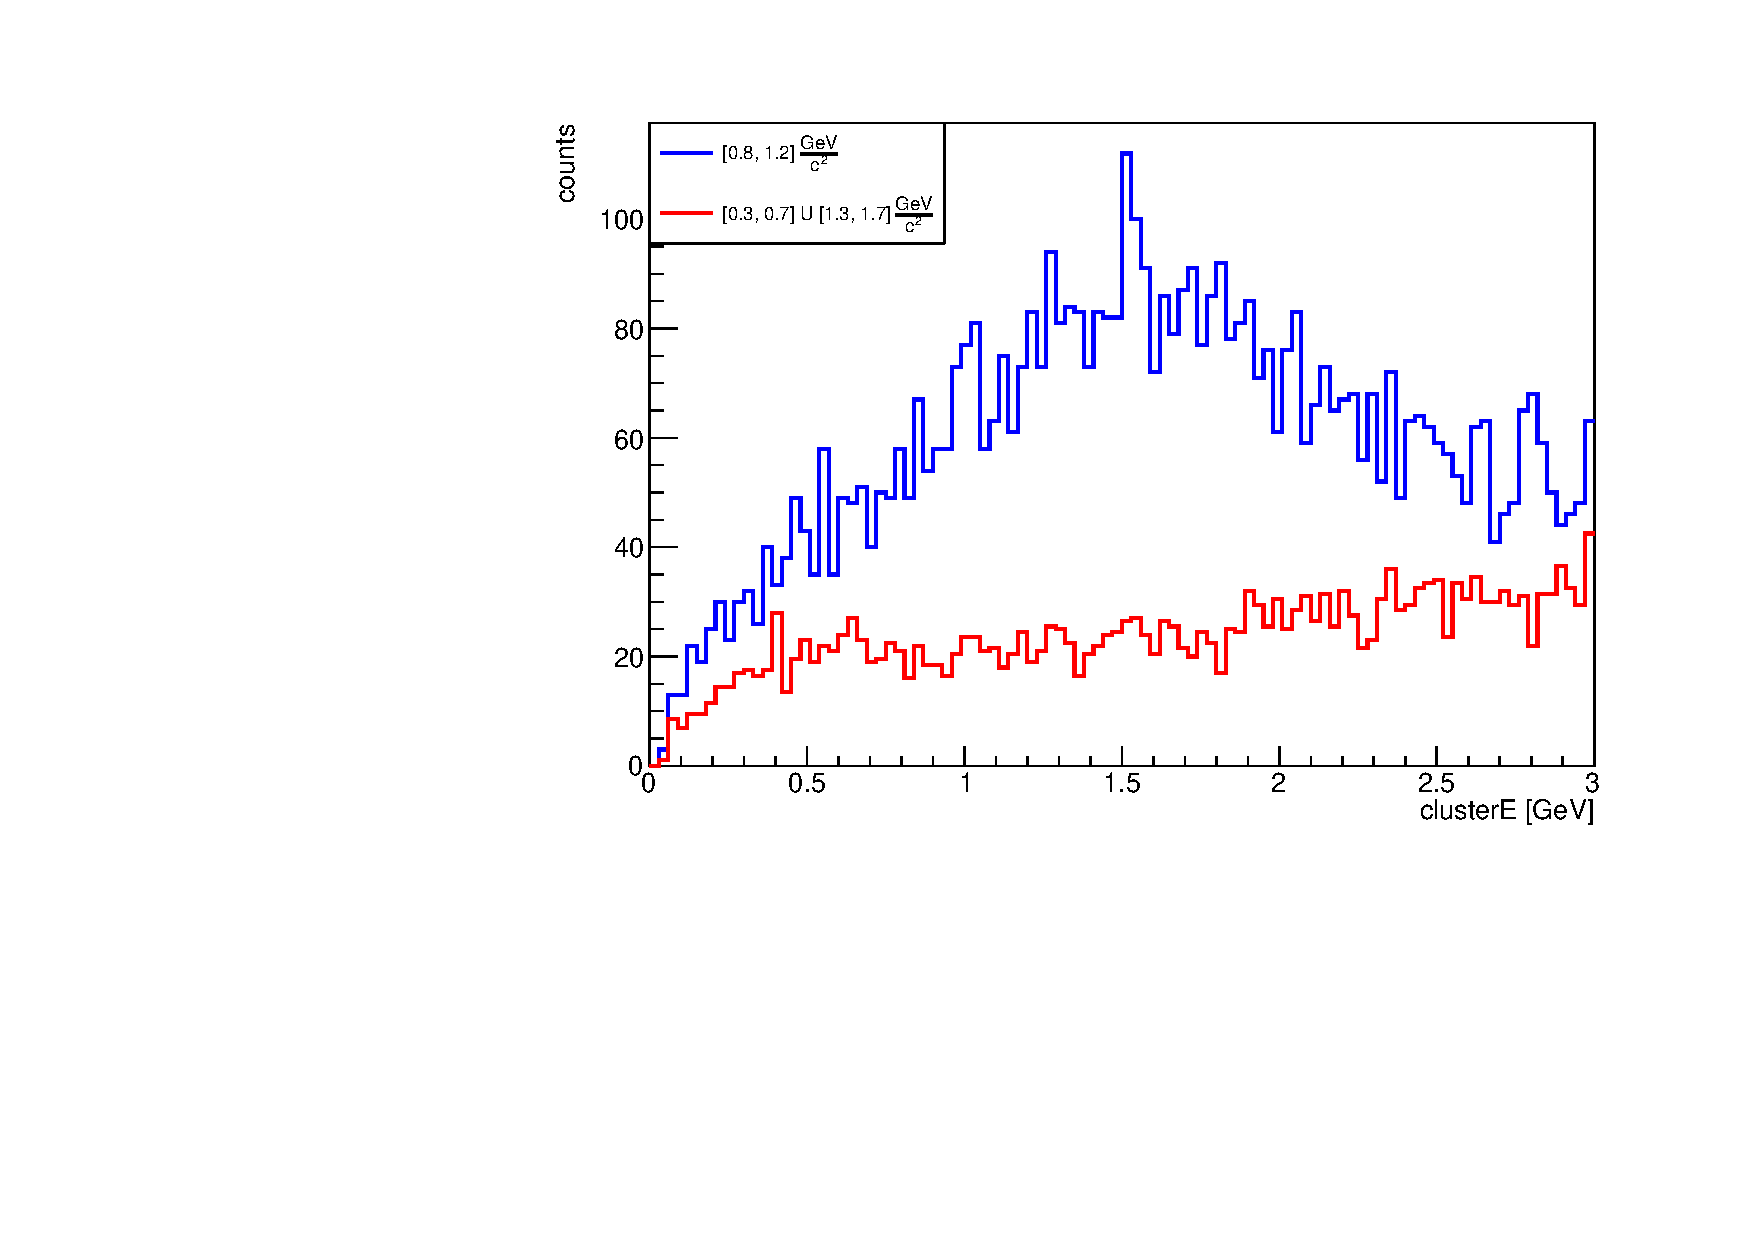
\includegraphics[width=0.49\textwidth]{nbar_cocktail/images/sidebands_clusterE_nog.pdf}
    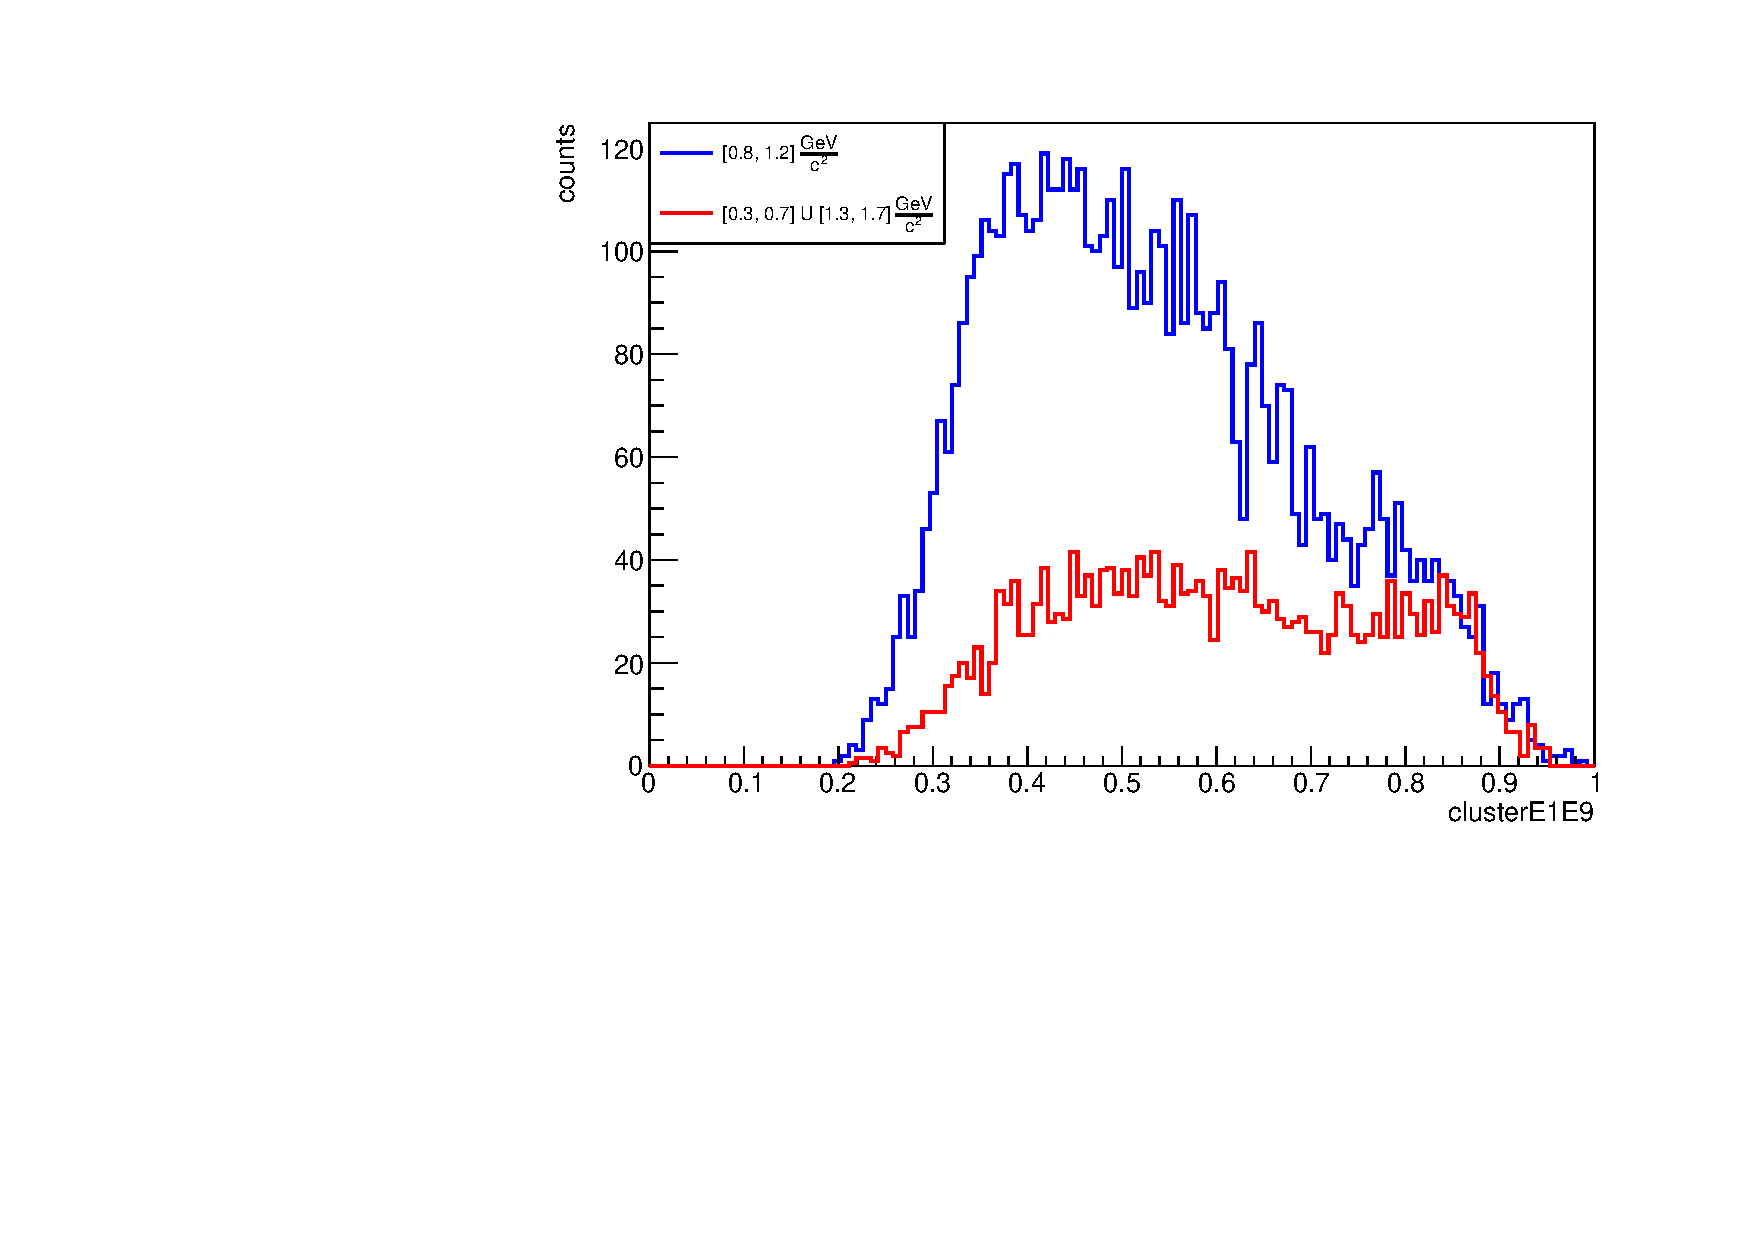
\includegraphics[width=0.49\textwidth]{nbar_cocktail/images/sidebands_clusterE1E9_nog.pdf}
    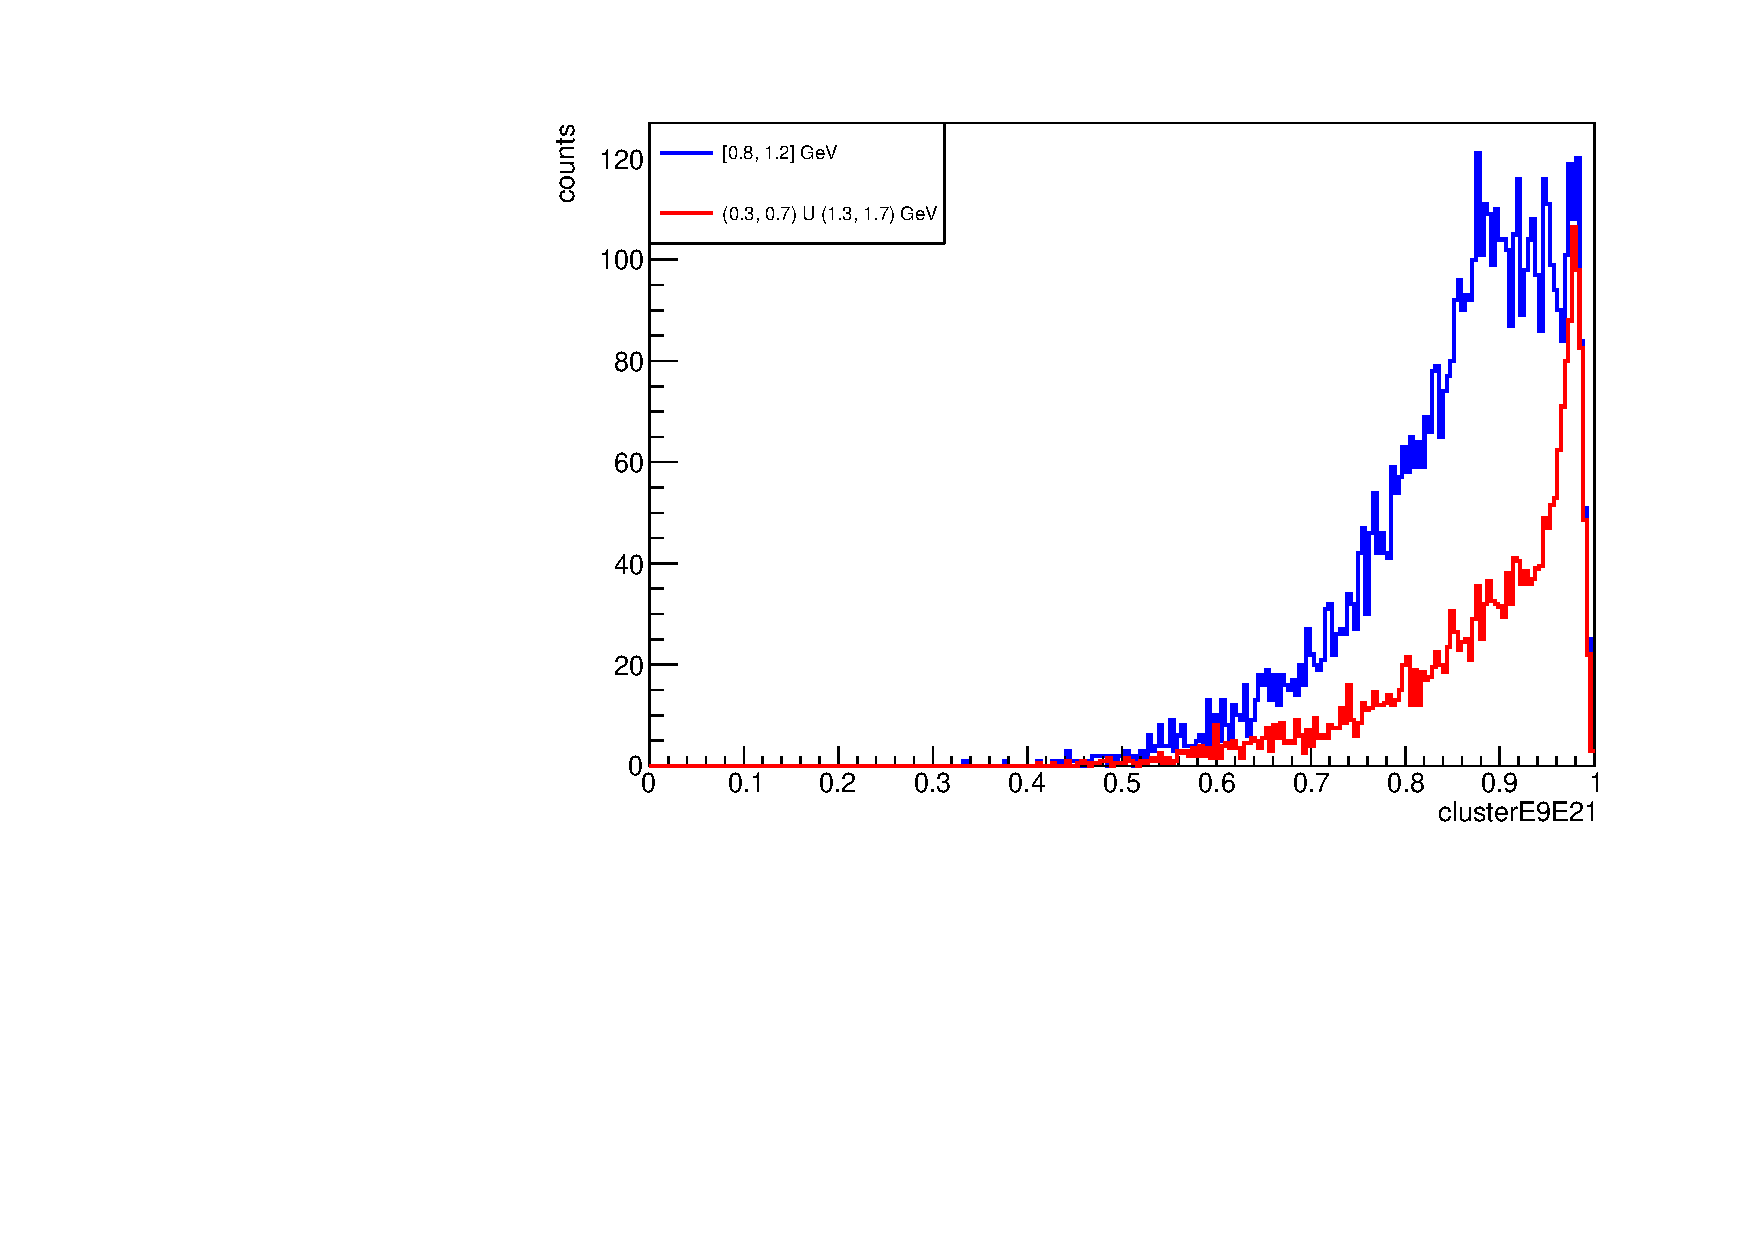
\includegraphics[width=0.49\textwidth]{nbar_cocktail/images/sidebands_clusterE9E21_nog.pdf}
    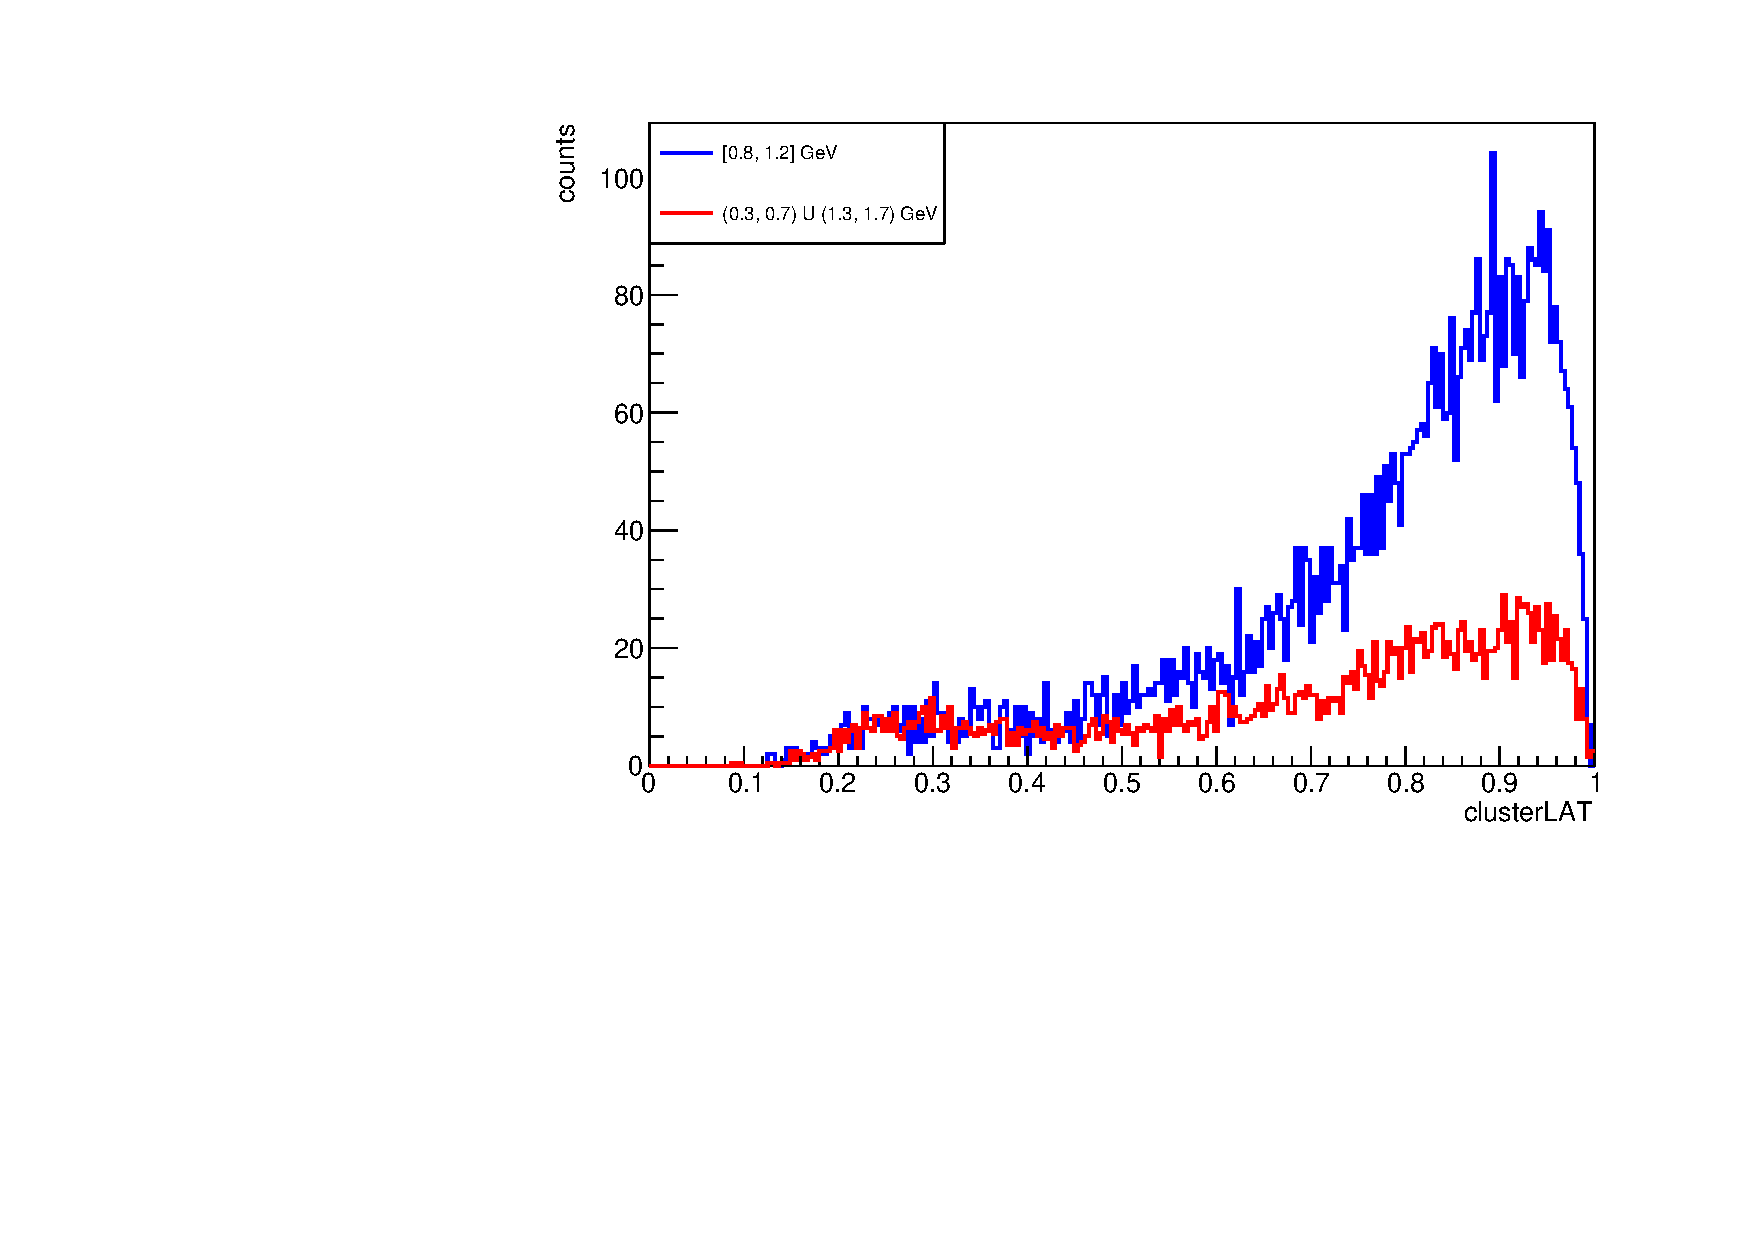
\includegraphics[width=0.49\textwidth]{nbar_cocktail/images/sidebands_clusterLAT_nog.pdf}
    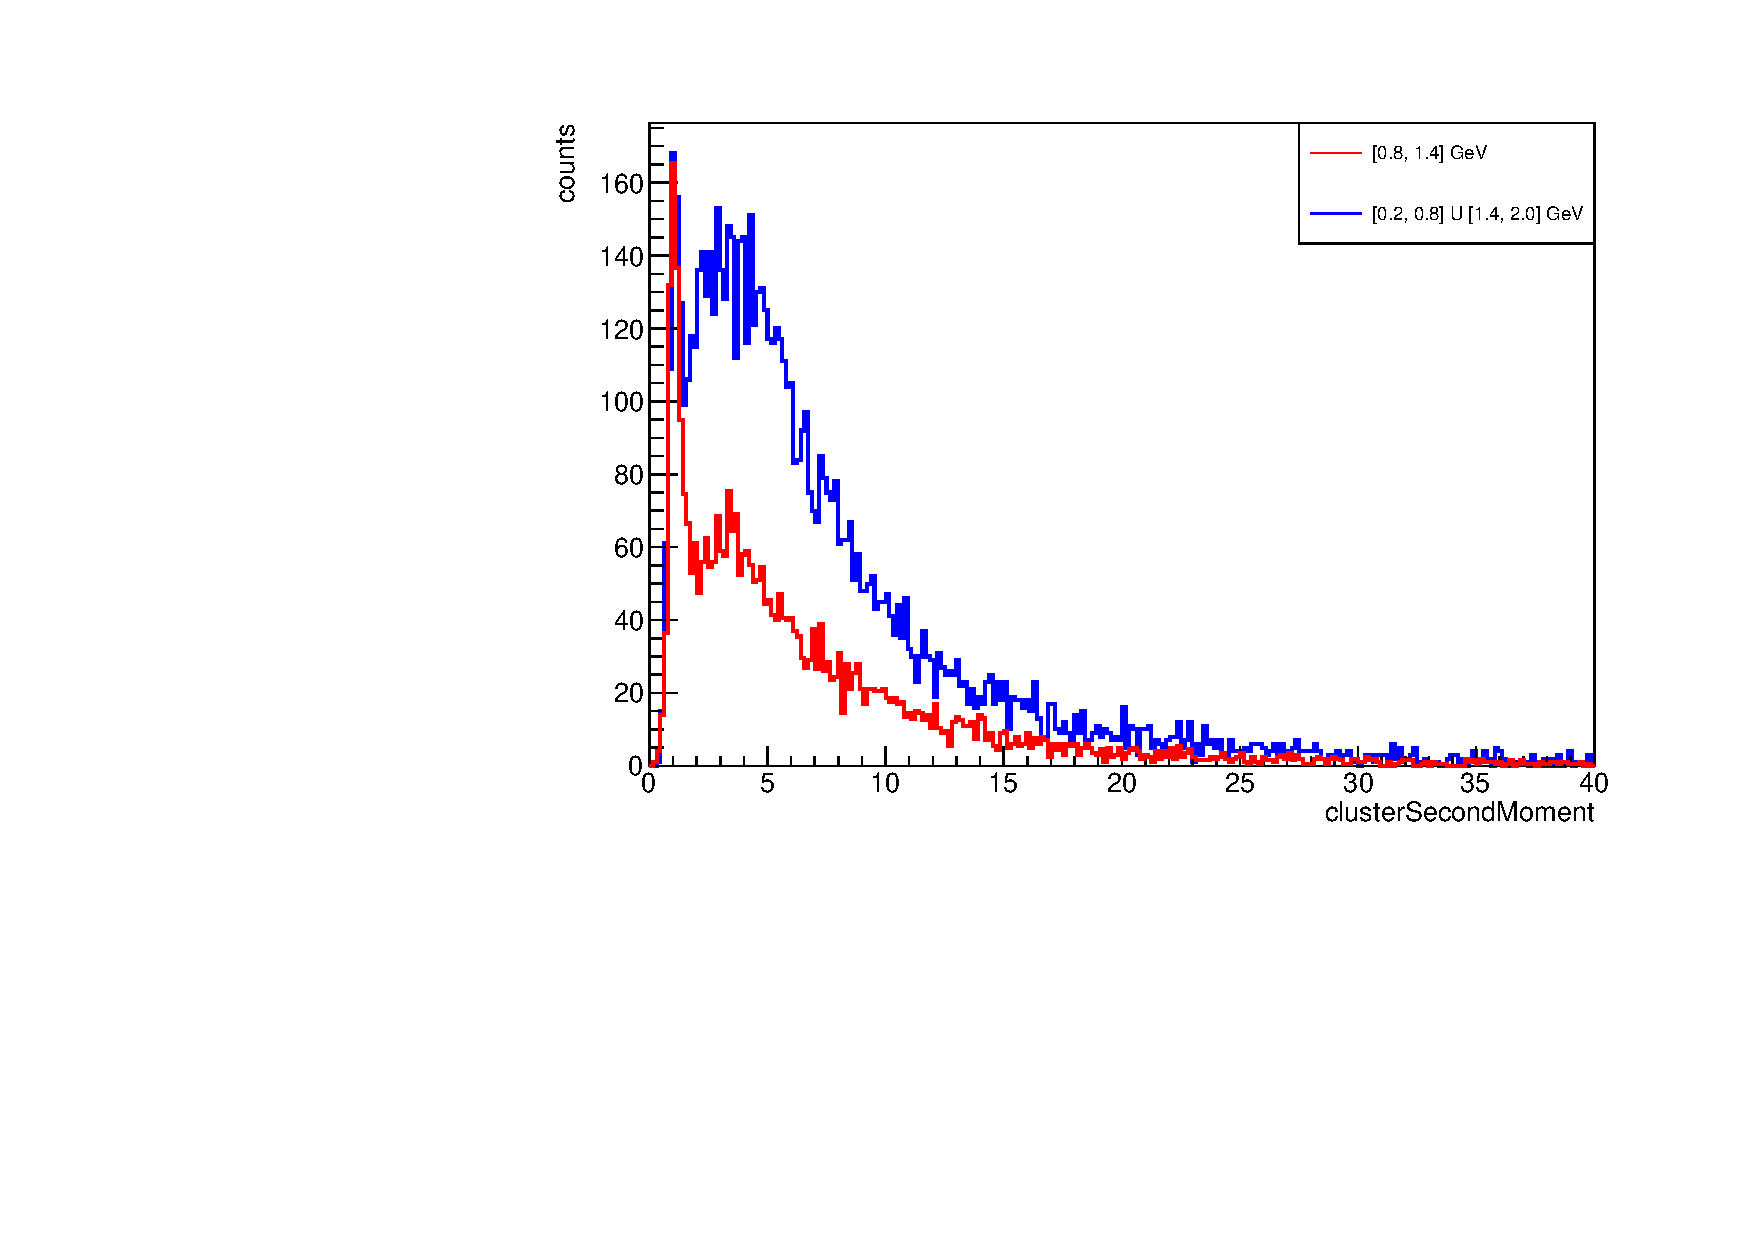
\includegraphics[width=0.49\textwidth]{nbar_cocktail/images/sidebands_clusterSecondMoment_nog.pdf}
    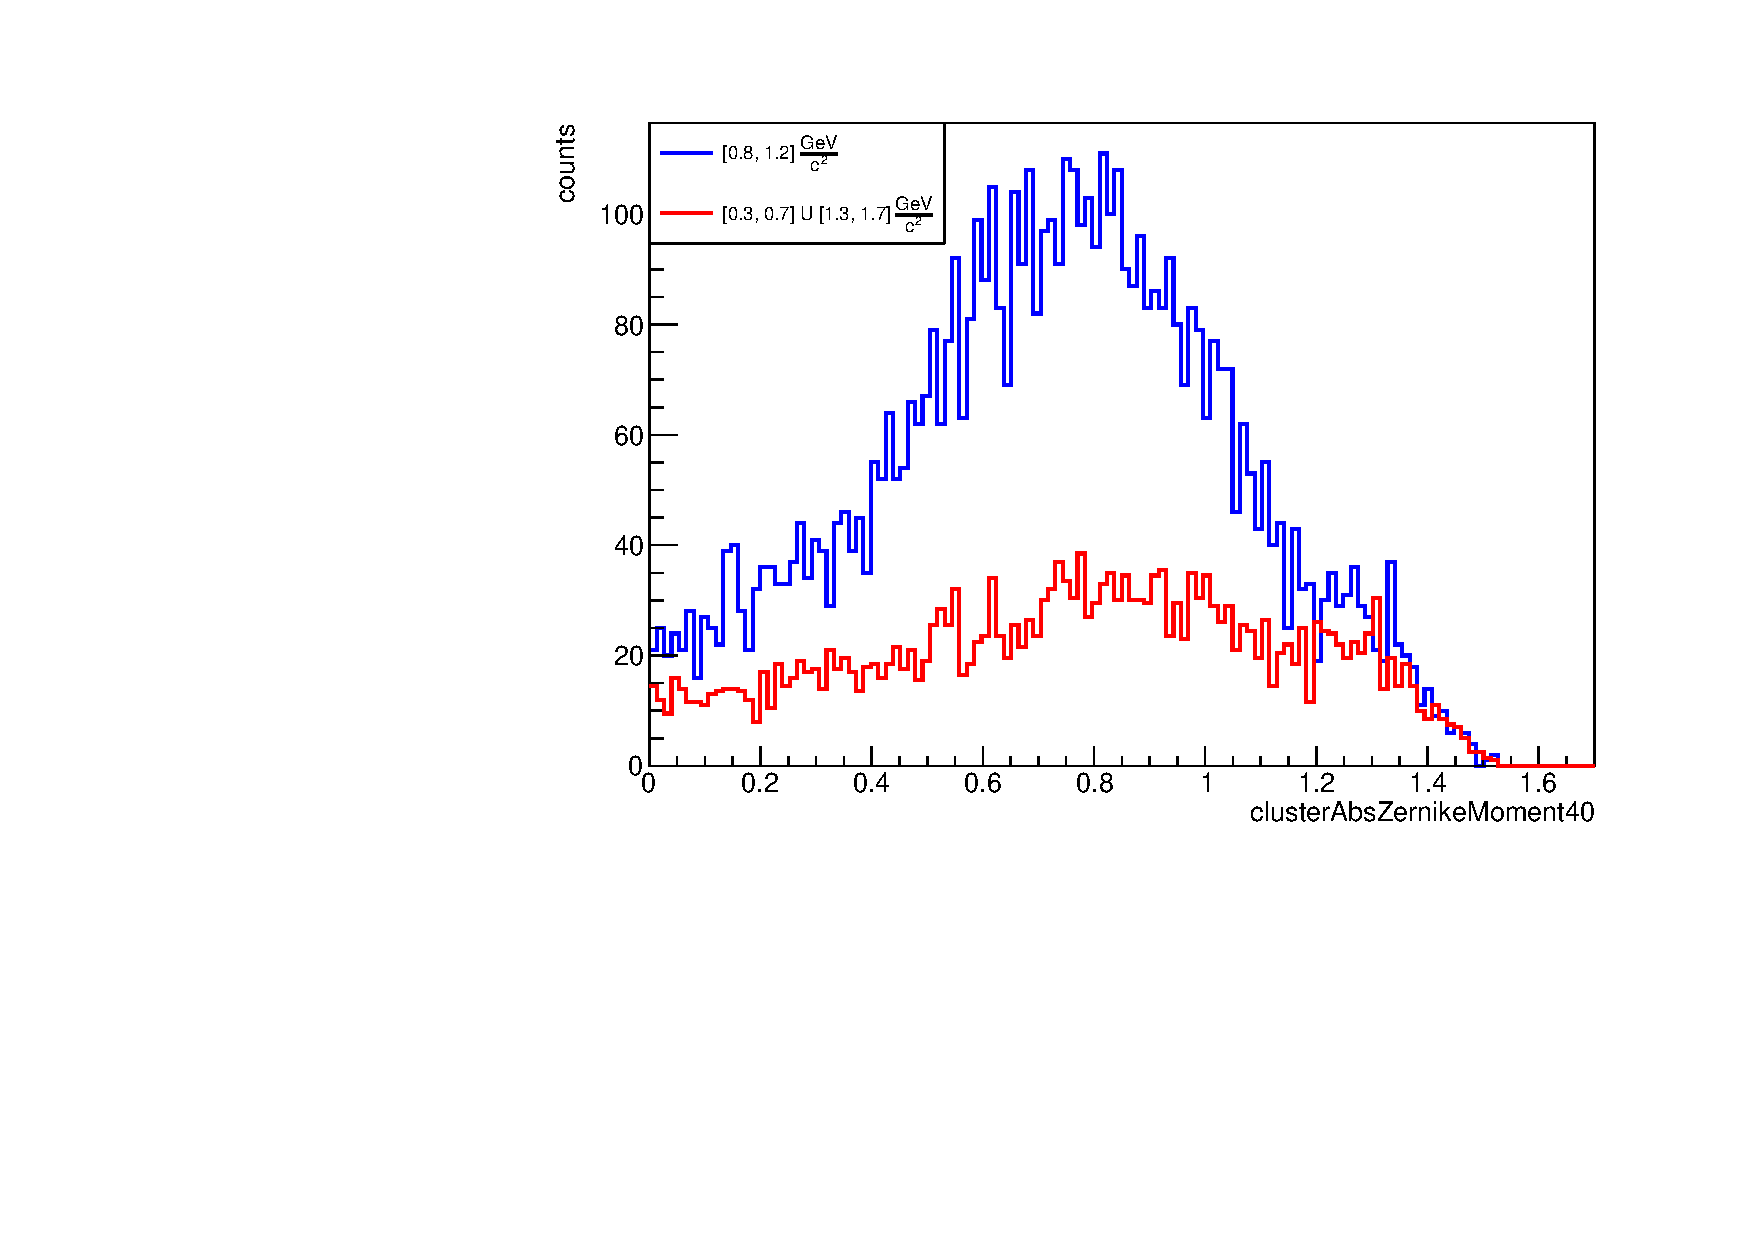
\includegraphics[width=0.49\textwidth]{nbar_cocktail/images/sidebands_clusterAbsZernikeMoment40_nog.pdf}
    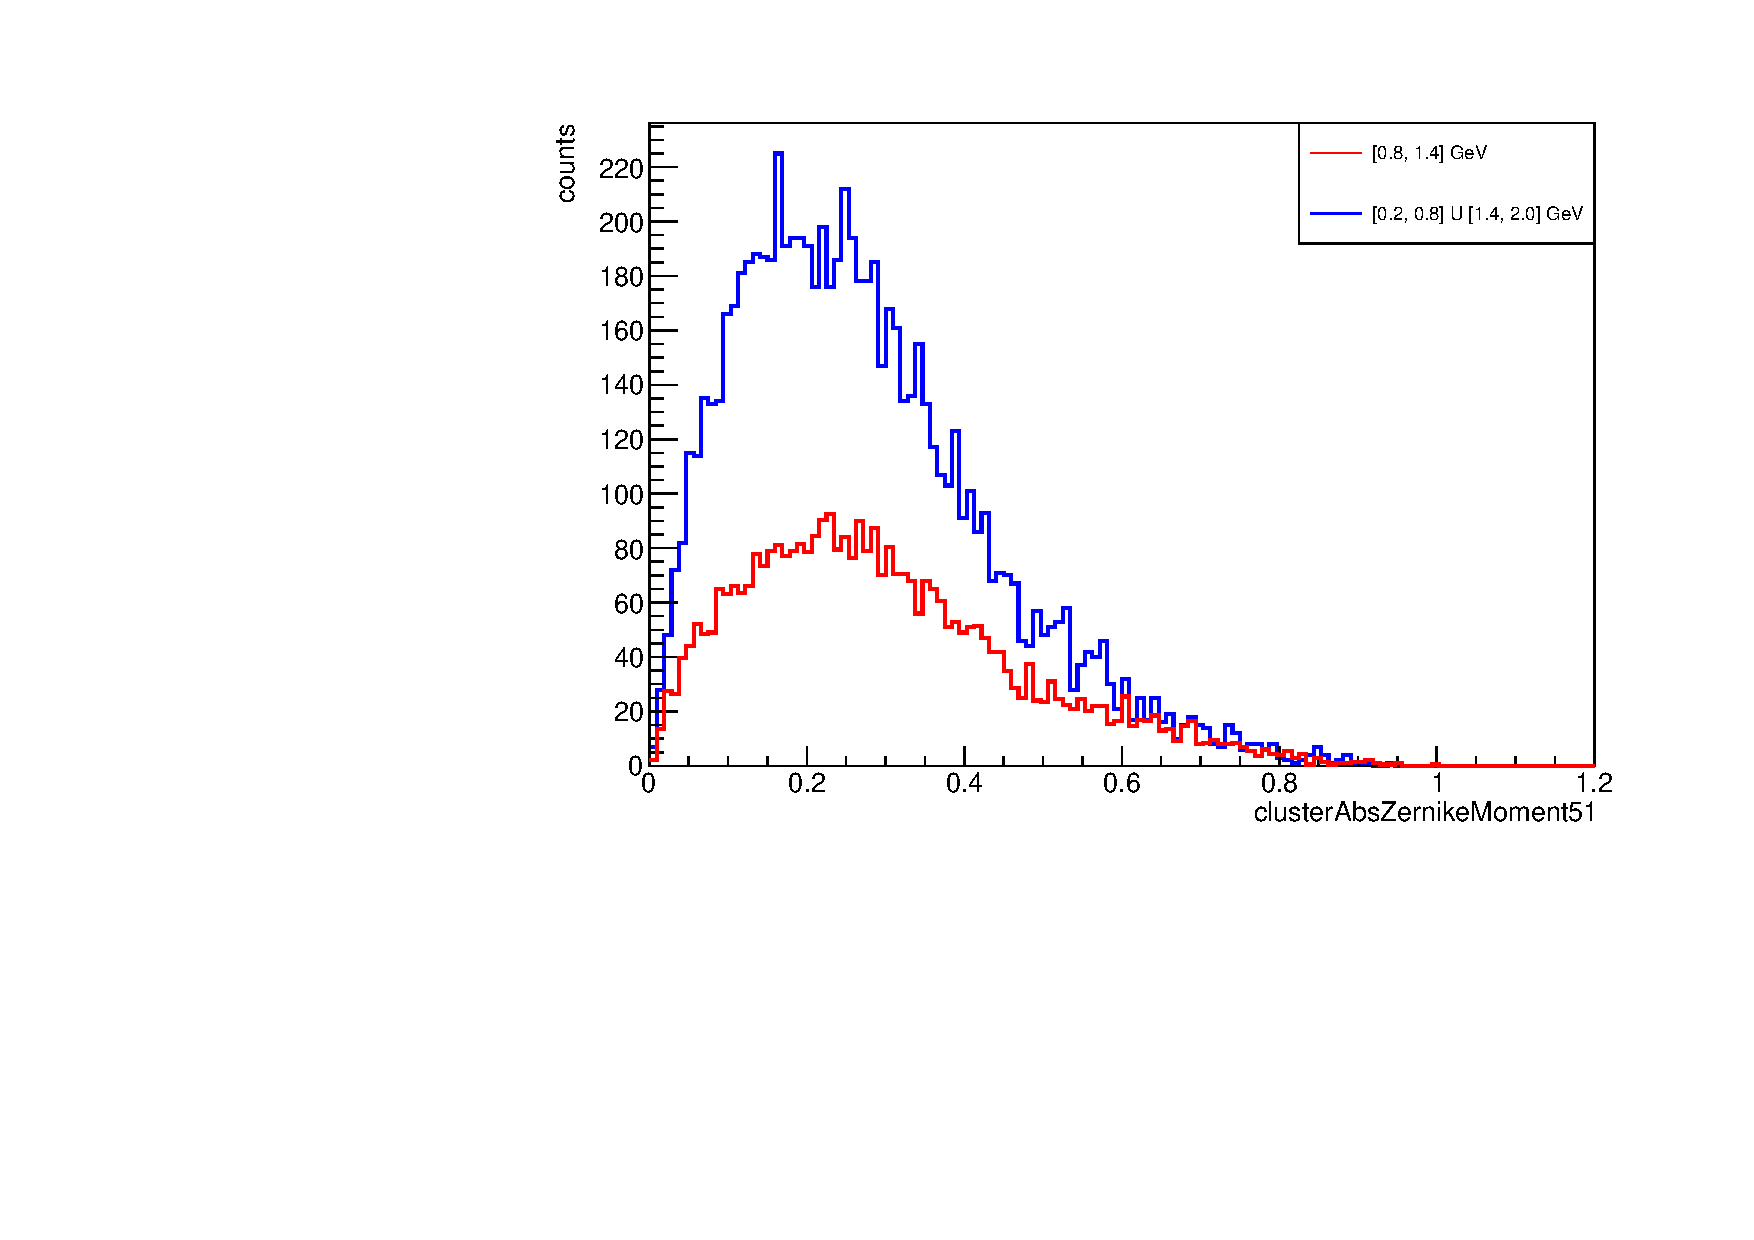
\includegraphics[width=0.49\textwidth]{nbar_cocktail/images/sidebands_clusterAbsZernikeMoment51_nog.pdf}
    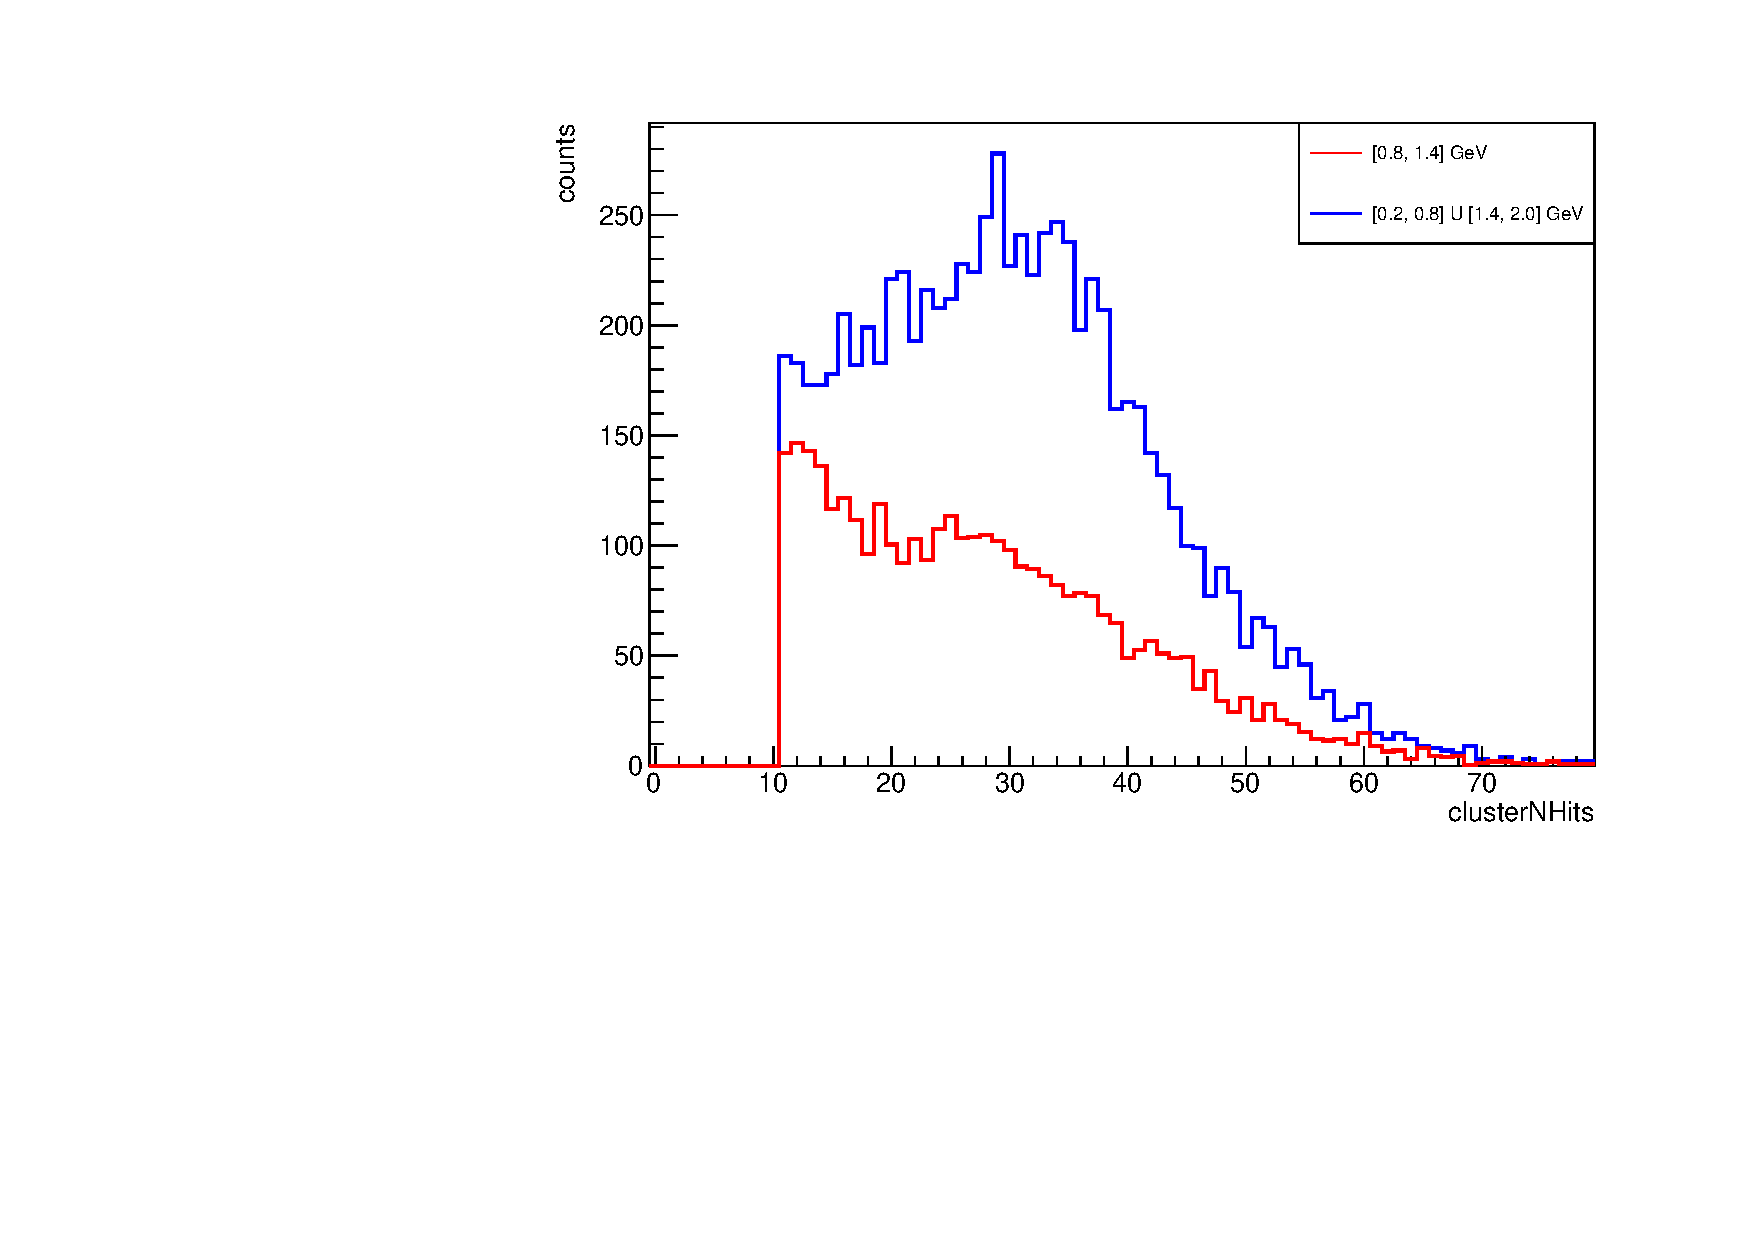
\includegraphics[width=0.49\textwidth]{nbar_cocktail/images/sidebands_clusterNHits_nog.pdf}
     \caption{Comparison of reconstructed cluster variables for $\bar{n}$ candidates in the signal region [0.8, 1.2] GeV (blue) with $\bar{n}$ candidates in the sidebands region [0.3, 0.7] U [1.3, 1.7]  GeV  (red), in NO ISR case. A scaling factor of $k = 0.5$ has been applied to the cluster variables obtained from the sidebands regions. q$\bar{q}$ cocktail.}
     \label{fig:clus_vars_sidebands_pre}
\end{figure}
$\\$
The cluster energy distribution shows a flat contribution from the sidebands regions, where no specific structure was observed. The E1E9 distribution shows that the structure observed in $\sim 0.85$ (Fig.~\ref{fig:clus_vars_nog_qqbar}) is mainly caused by background components, such as those coming from the sidebands regions. The same conclusion can be reached for the structure observed close to unity in the E9E21 distribution. 
$\\$
Furthermore, the sidebands regions provide the main contribution to the structure observed at low values in the Second Moment distribution, caused by small-sized clusters. 
$\\$
The cluster Zernike moment $Z^0_4$ presents a tail around $Z^0_4 \sim 1.2$ caused by sidebands contribution, while $Z^1_5$ presents no discernible structure.
$\\$
Afterwards, the structure observed at a value of $\sim 0.3$ in the Lateral Momentum distribution is caused by sidebands contribution.
$\\$
Therefore, to obtain the final $\bar{n}$ candidates cluster variables distribution, the sidebands regions contribution (background) is subtracted from the signal region contribution (signal + background). The obtained cluster variables are shown in Fig.\ref{fig:clus_vars_sidebands_post}.

 \begin{figure}[h]
    \centering
    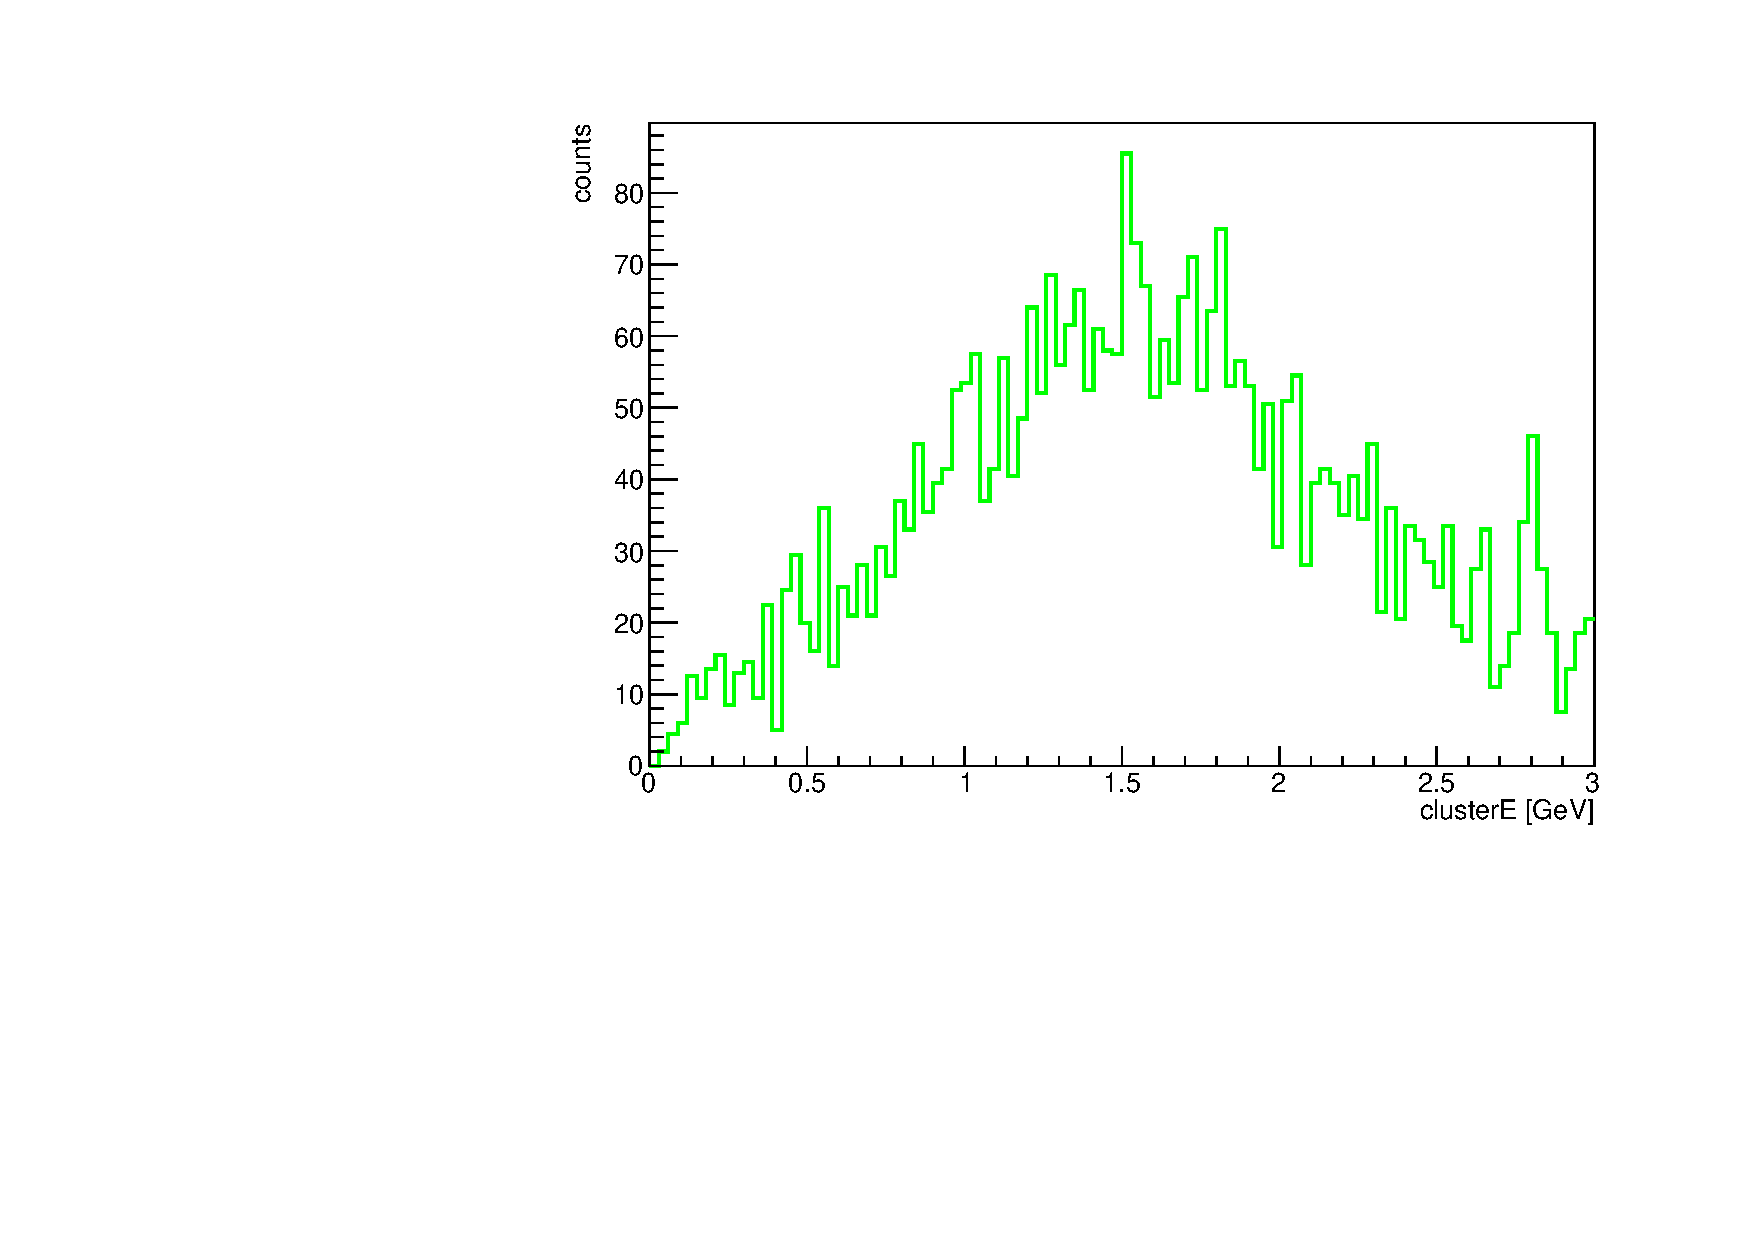
\includegraphics[width=0.49\textwidth]{nbar_cocktail/images/final_clusterE_nog.pdf}
    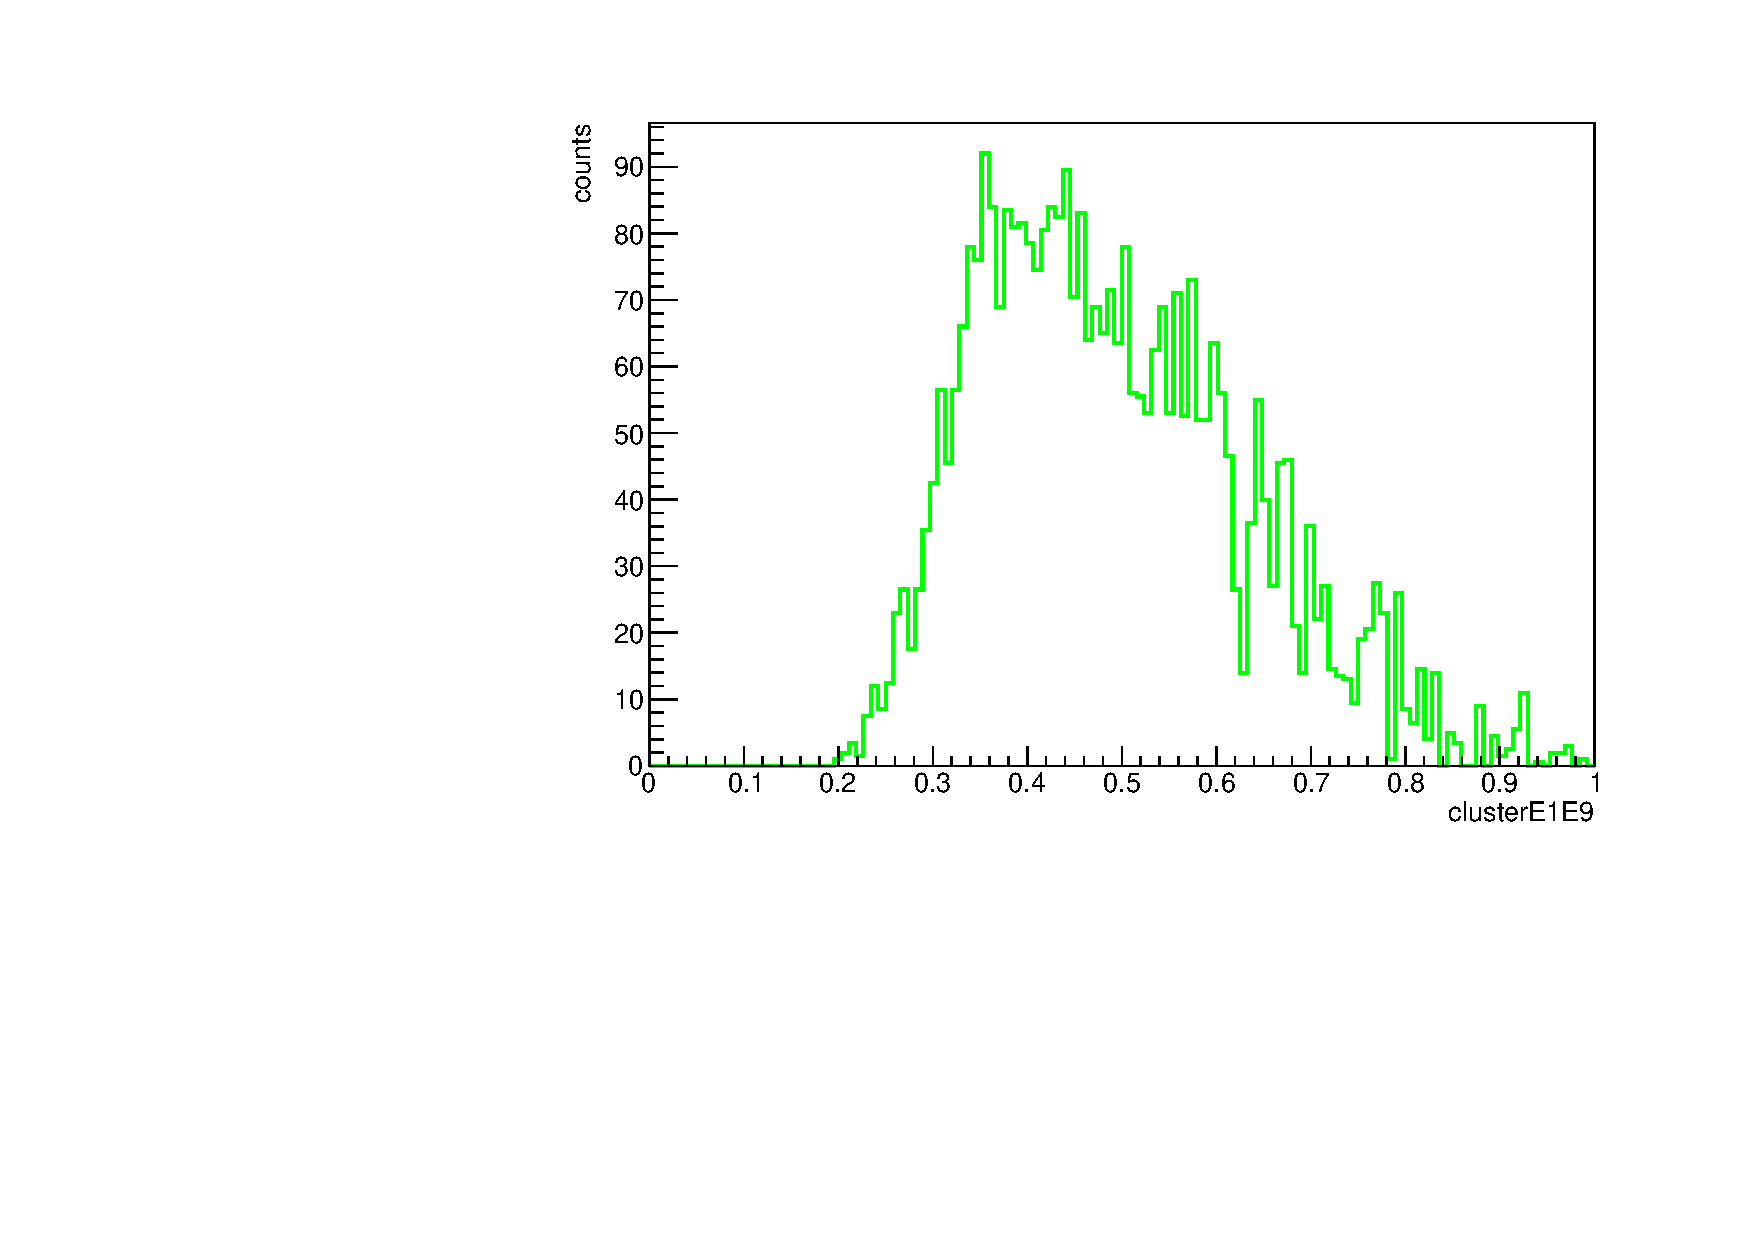
\includegraphics[width=0.49\textwidth]{nbar_cocktail/images/final_clusterE1E9_nog.pdf}
    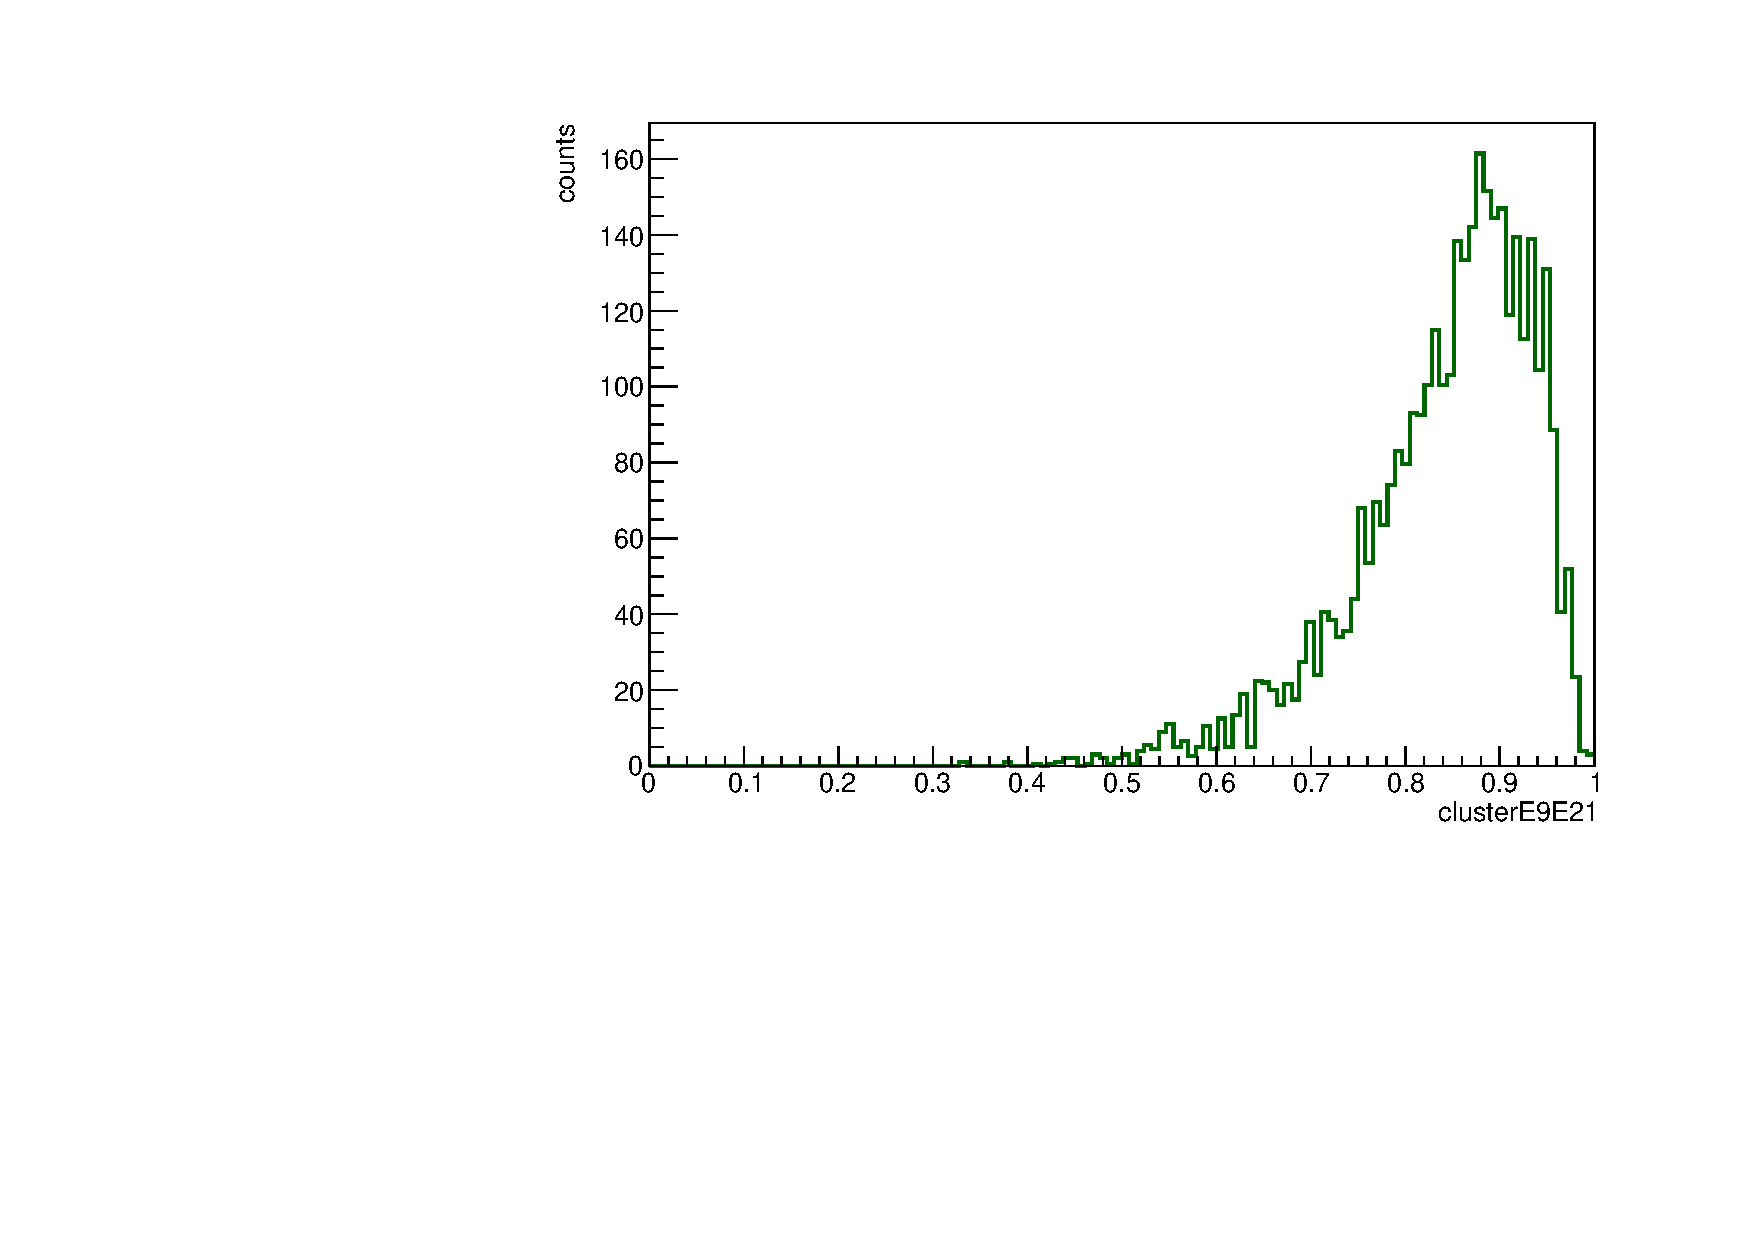
\includegraphics[width=0.49\textwidth]{nbar_cocktail/images/final_clusterE9E21_nog.pdf}
    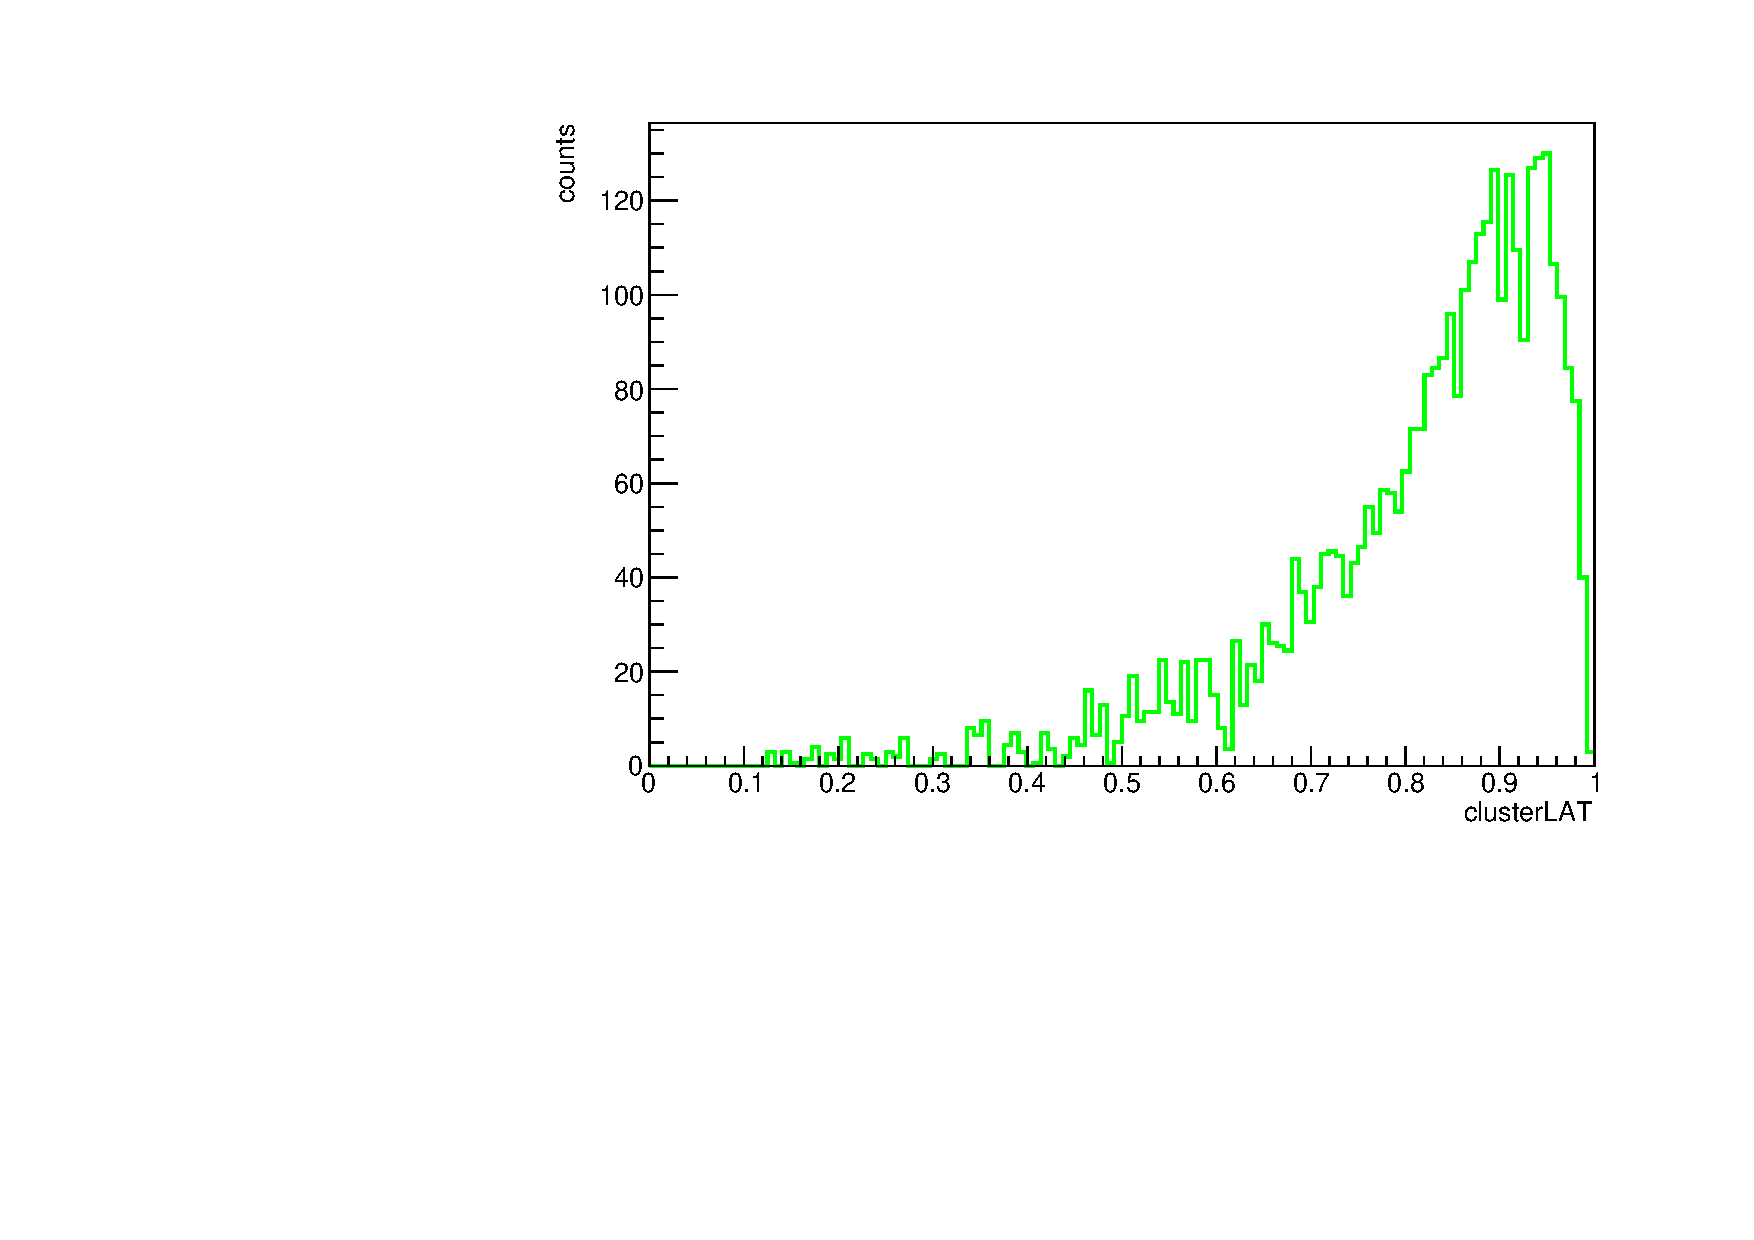
\includegraphics[width=0.49\textwidth]{nbar_cocktail/images/final_clusterLAT_nog.pdf}
    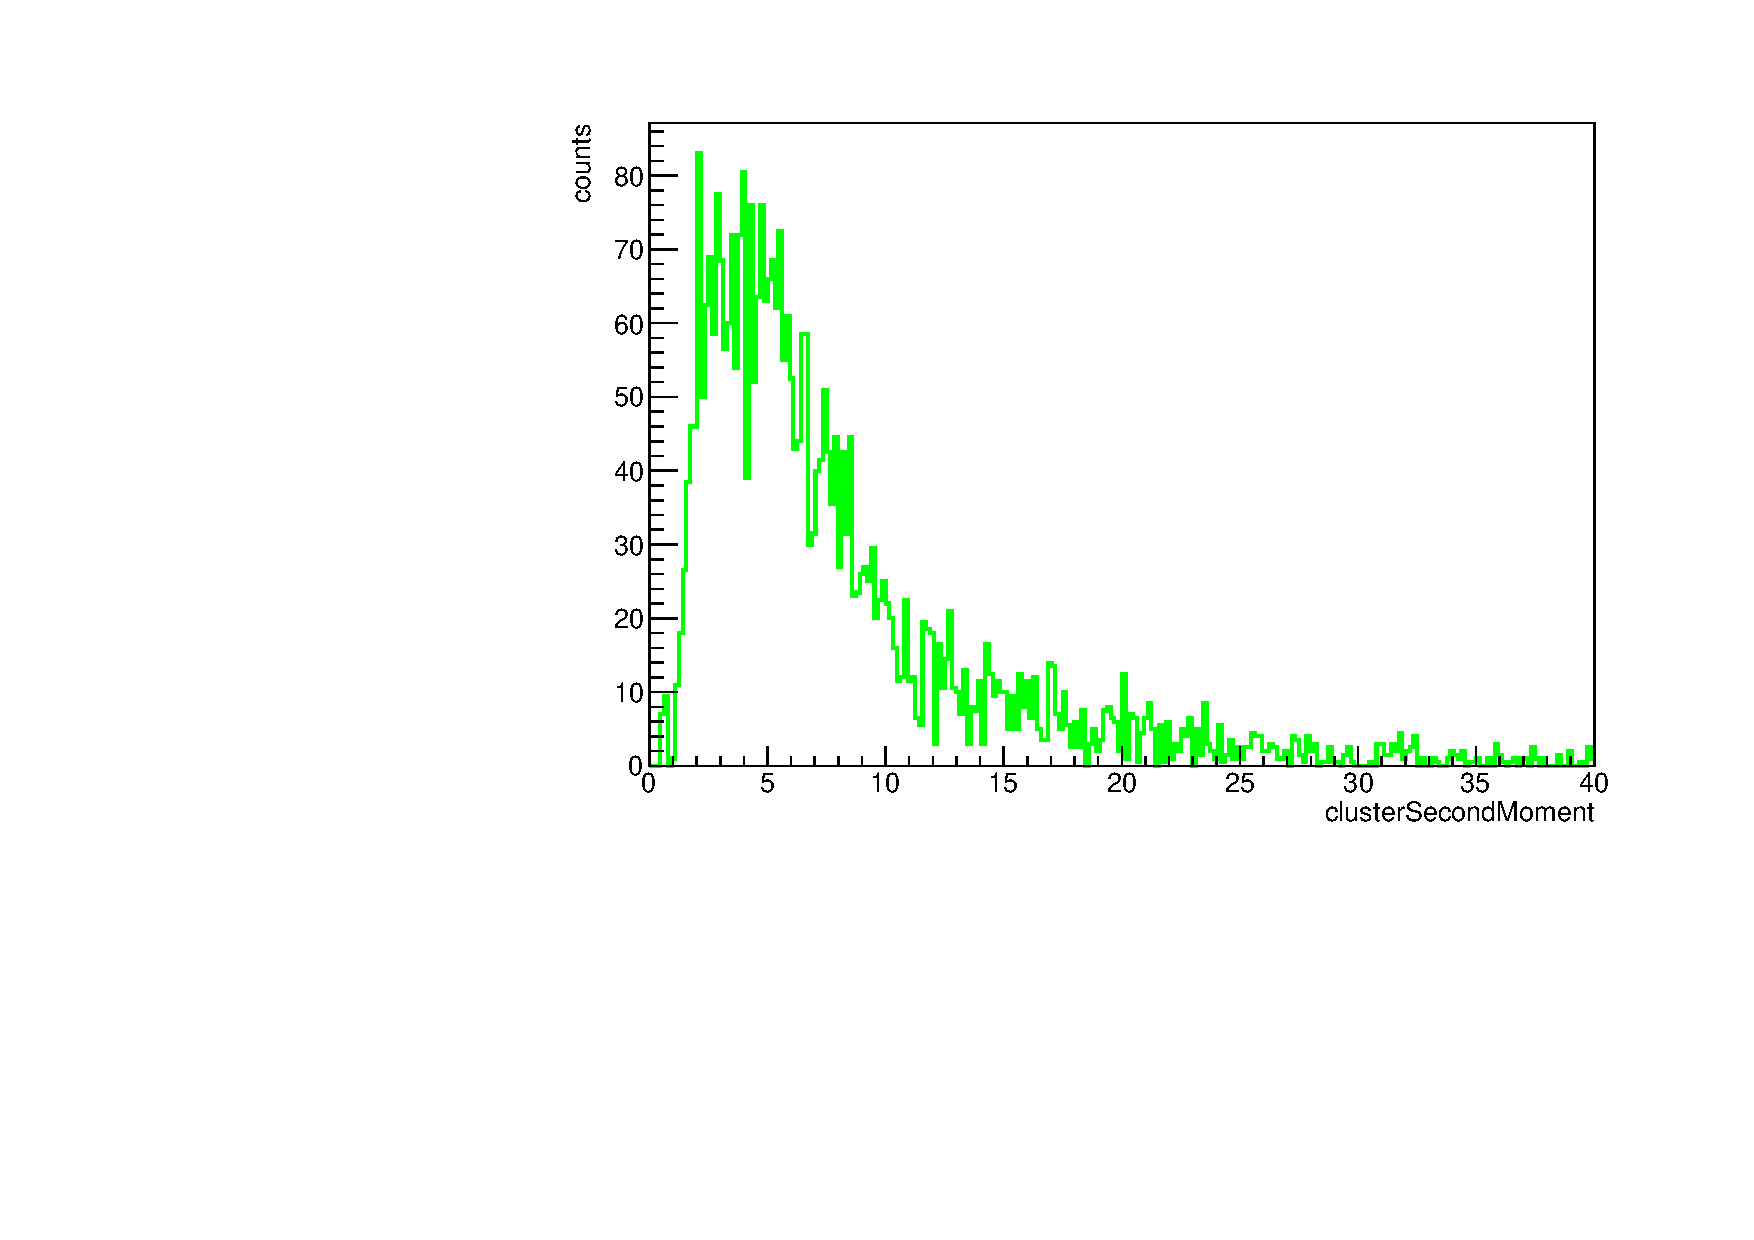
\includegraphics[width=0.49\textwidth]{nbar_cocktail/images/final_clusterSecondMoment_nog.pdf}
    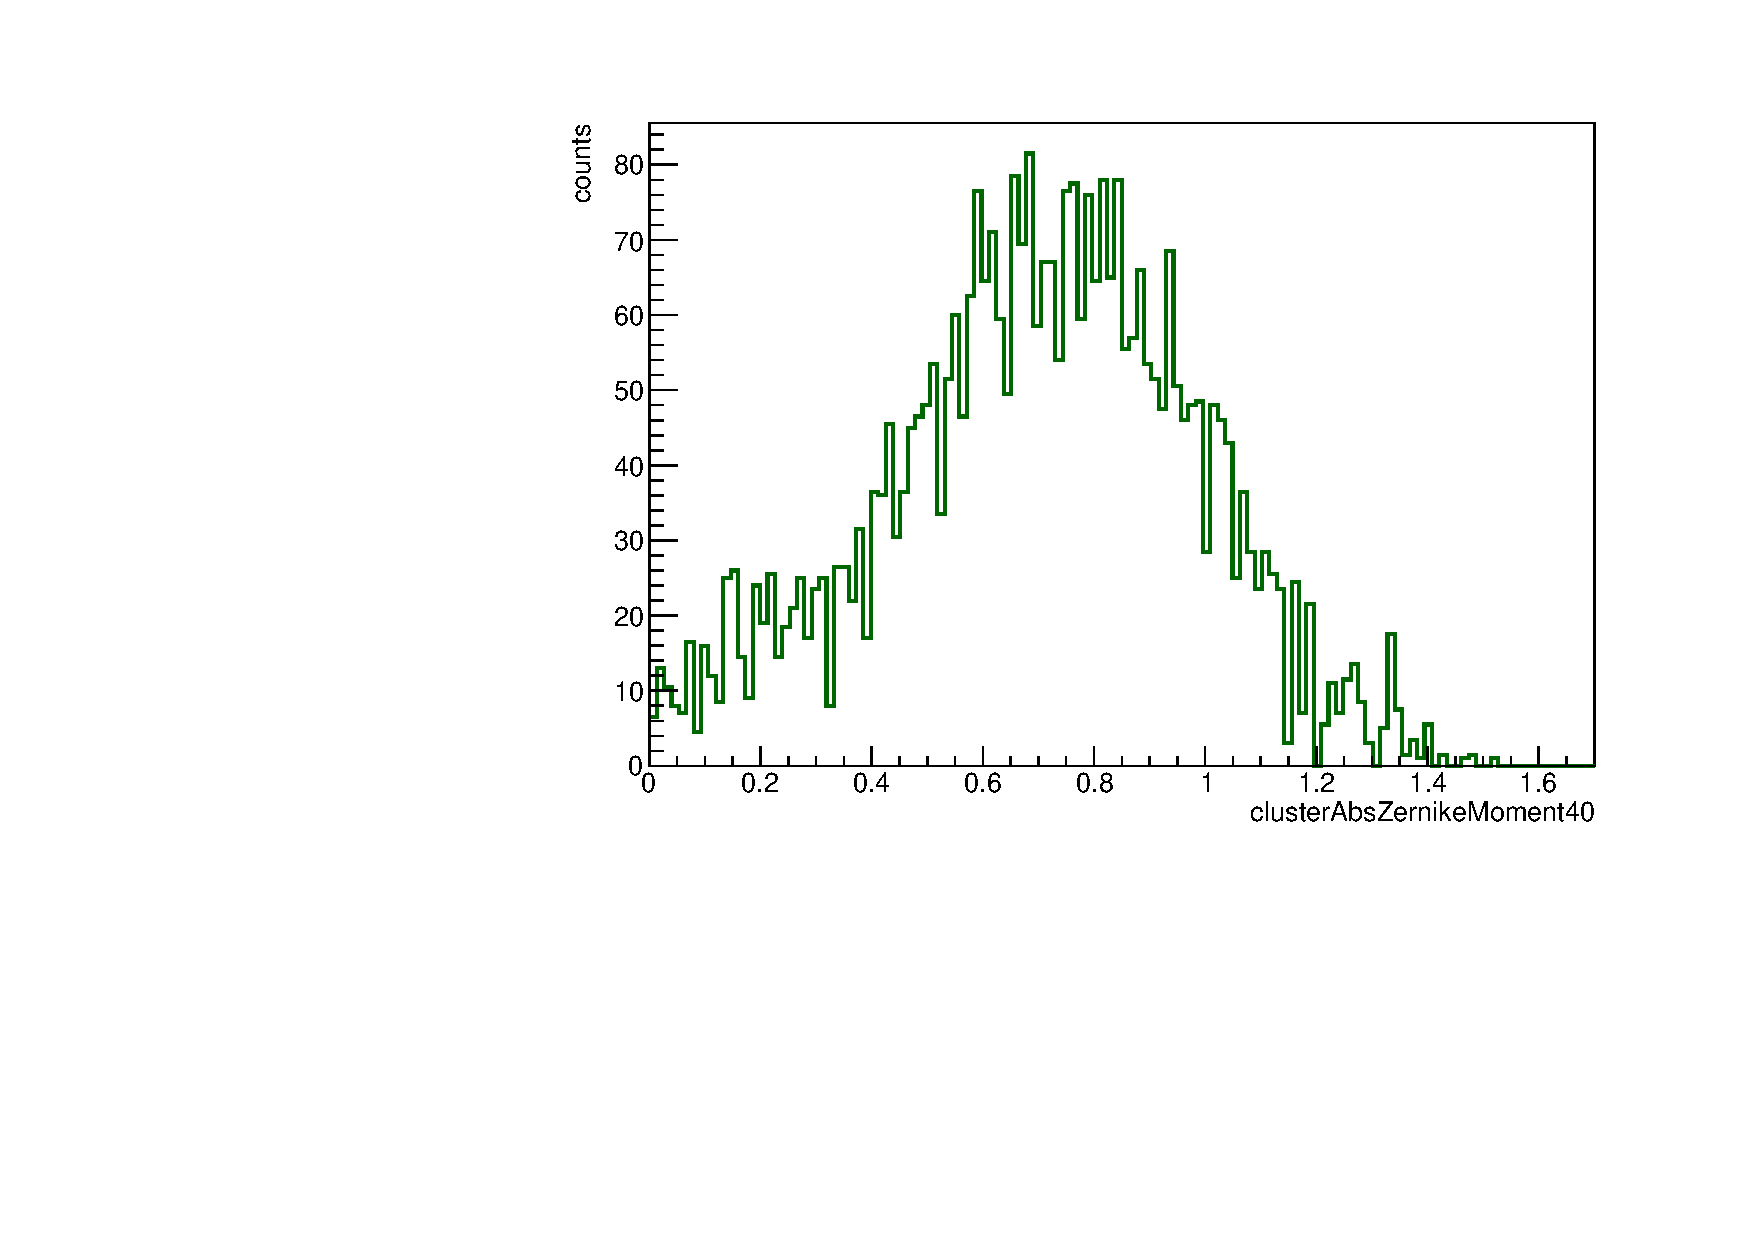
\includegraphics[width=0.49\textwidth]{nbar_cocktail/images/final_clusterAbsZernikeMoment40_nog.pdf}
    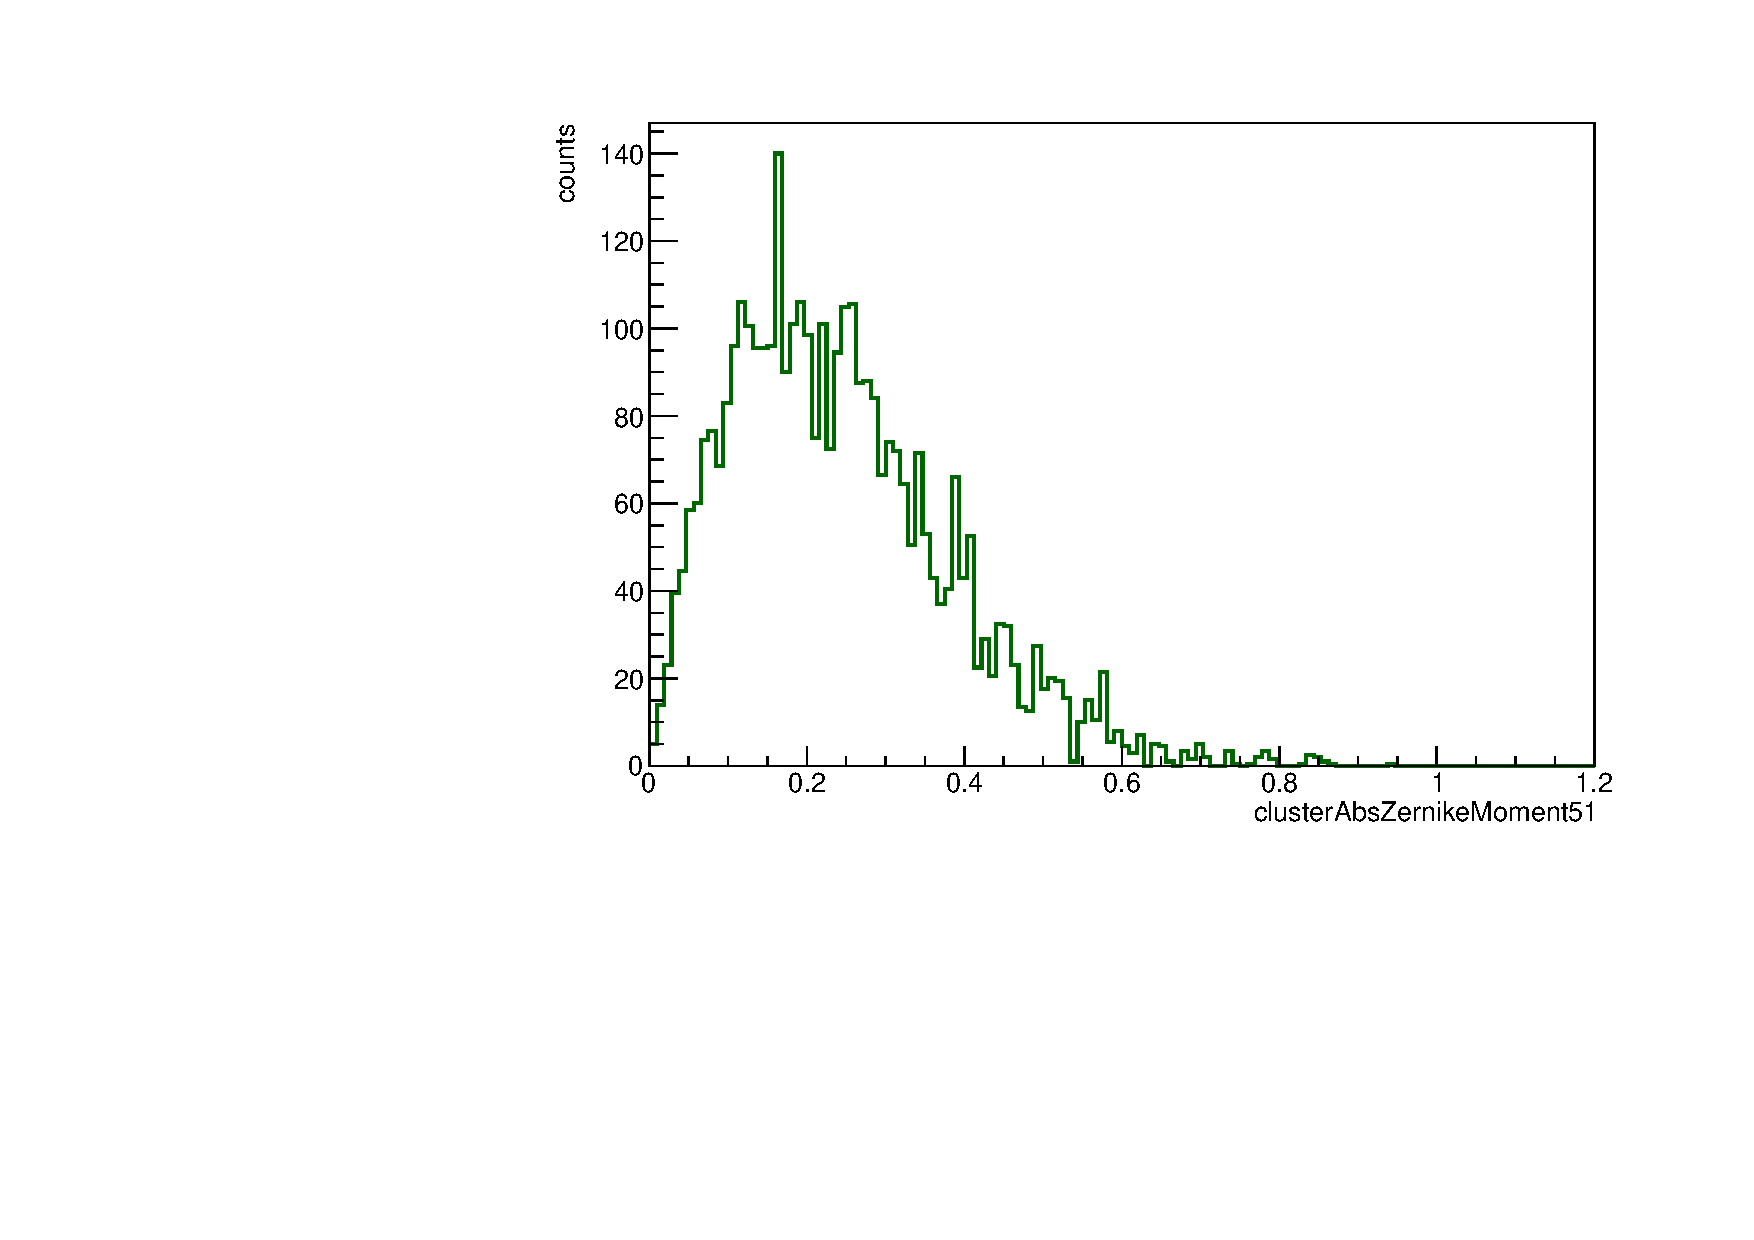
\includegraphics[width=0.49\textwidth]{nbar_cocktail/images/final_clusterAbsZernikeMoment51_nog.pdf}
    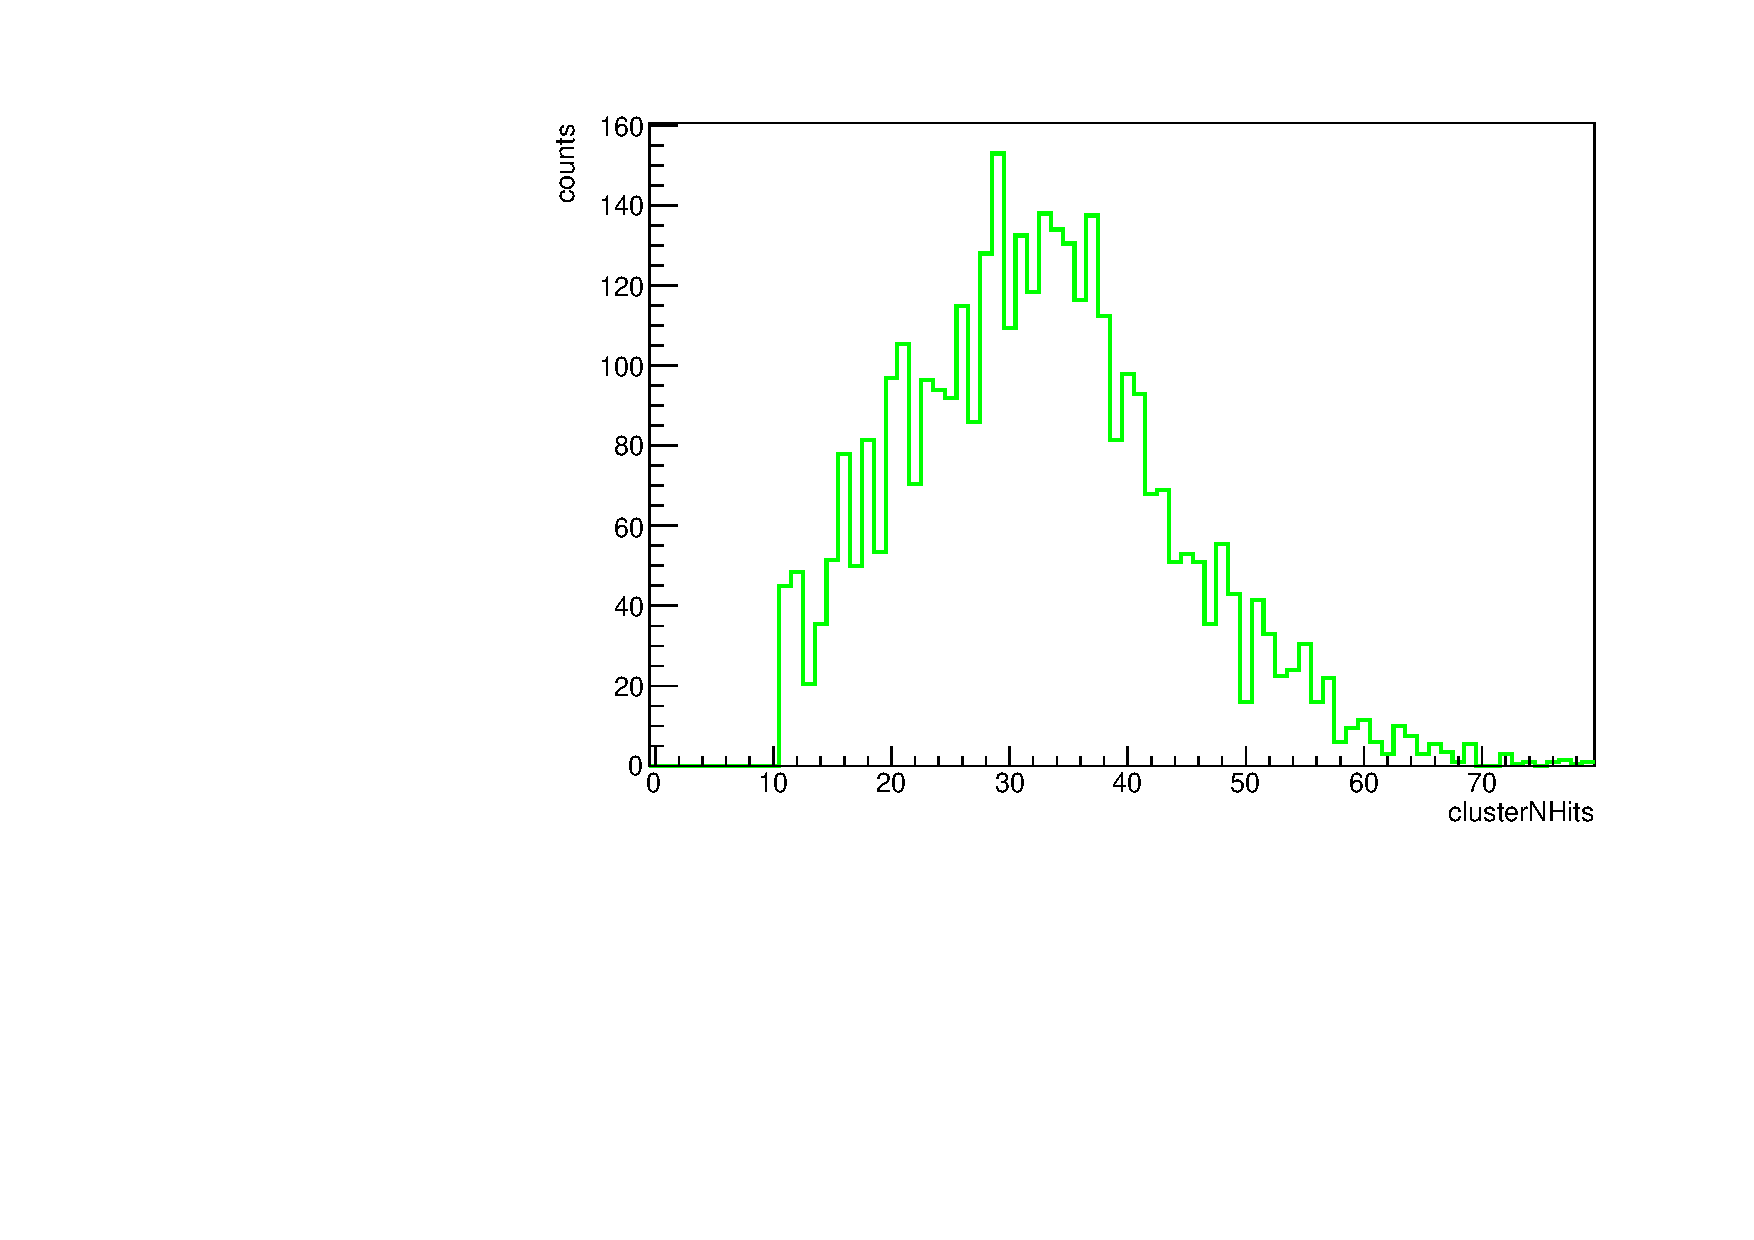
\includegraphics[width=0.49\textwidth]{nbar_cocktail/images/final_clusterNHits_nog.pdf}
   
     \caption{Reconstructed cluster variables for $\bar{n}$ candidates after the application of the sidebands technique, in NO ISR case. q$\bar{q}$ cocktail.}
     \label{fig:clus_vars_sidebands_post}
\end{figure}

The obtained cluster variables distributions no longer present the singular structures observed prior to the sidebands technique application. This leads to reconstructed cluster variables more similar to those obtained from the Monte Carlo signal sample analysis (Fig.~\ref{fig:clus_vars_2}). This suggests that the applied selections and the sidebands technique properly separate the signal contribution from the background one, in q$\bar{q}$ cocktail, with no explicit $\gamma_{ISR}$ reconstruction.

\subsection{$q\bar{q}$ cocktail production (ISR case)}
Since the same path as the NO ISR case has been followed, in the ISR case the $q\bar{q}$ cocktail is directly analyzed. The same final selections adopted in the NO ISR case have been used.
$\\$
The TopoAna output of can be consulted in Fig.~\ref{fig:topo_isr_010_qqbar}.
\begin{figure}[H]
    \centering
    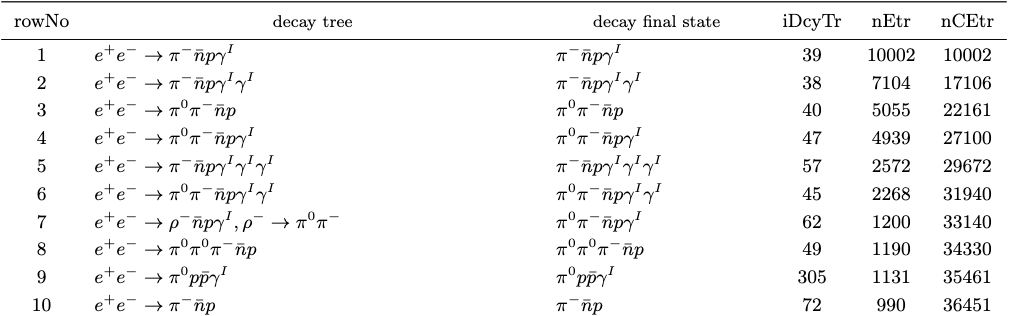
\includegraphics[width=1\textwidth]{nbar_cocktail/images/topoana_isr_010_qqbar}
    \caption{First 10 channels of the TopoAna output in $q\bar{q}$ Monte Carlo cocktail, showing the different channel contributes. ISR case.}
    \label{fig:topo_isr_010_qqbar}
\end{figure}
The TopoAna output reveals a situation very similar to that obtained in the NO ISR case. In fact, now, the dominant contribution is from the signal channel $p \pi^- \bar{n} \gamma_{ISR}$. A secondary contribution comes from $p \pi^- \bar{n} \gamma_{ISR}  \gamma_{ISR}$, which could be treated as signal despite the extra $\gamma_{\text{ISR}}$ not being explicitly reconstructed. The next contribution comes from $p \pi^- \bar{n} \pi^0$ in the final state. The fourth contribution is due to $p \pi^- \bar{n} \pi^0 \gamma_{\text{ISR}}$, and so on. The individual TopoAna outputs from $u\bar{u}$, $d\bar{d}$, $s\bar{s}$ and $c\bar{c}$ are shown in Fig.~\ref{fig:topo_isr_010_qqbar_singles}.
\begin{figure}[H]
    \centering
    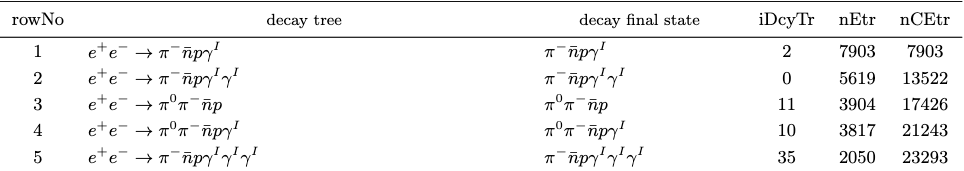
\includegraphics[width=1\textwidth]{nbar_cocktail/images/topo_uubar_isr}
    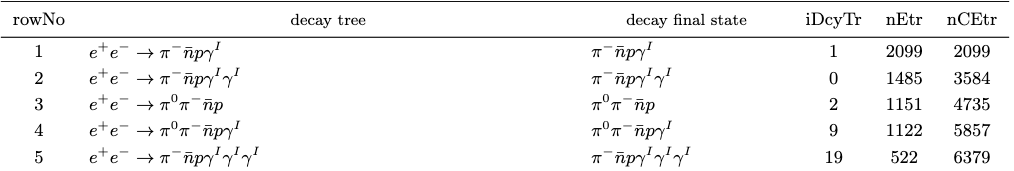
\includegraphics[width=1\textwidth]{nbar_cocktail/images/topo_ddbar_isr}
    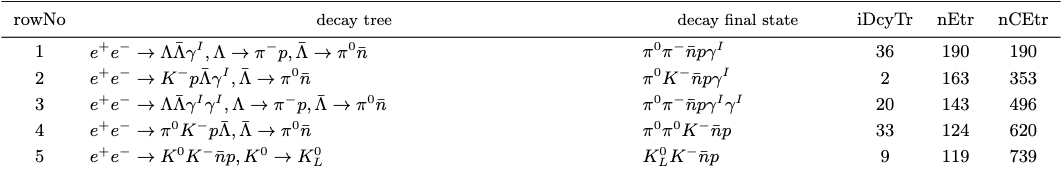
\includegraphics[width=1\textwidth]{nbar_cocktail/images/topo_ssbar_isr}
    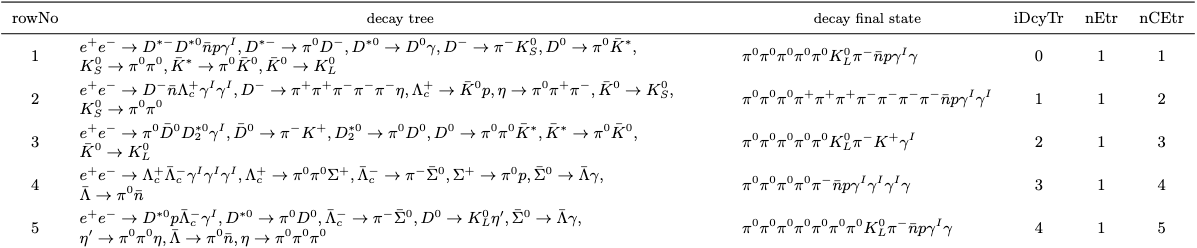
\includegraphics[width=1\textwidth]{nbar_cocktail/images/topo_ccbar_isr}
    \caption{Top 5 channels from the TopoAna output respectively for the $u\bar{u}$, $d\bar{d}$, $s\bar{s}$, and $c\bar{c}$ Monte Carlo cocktails (from top to bottom). ISR case.}
    \label{fig:topo_isr_010_qqbar_singles}
\end{figure}
As observed in the NO ISR case, the main contributions to the final signal state are from the $u\bar{u}$ and $d\bar{d}$ cocktails in the ISR case as well. The obtained stacked components to the recoil mass, in $q\bar{q}$ cocktail, are shown in figure ~\ref{fig:mRecComps_isr_010_qqbar}.
\begin{figure}[H]
    \centering
    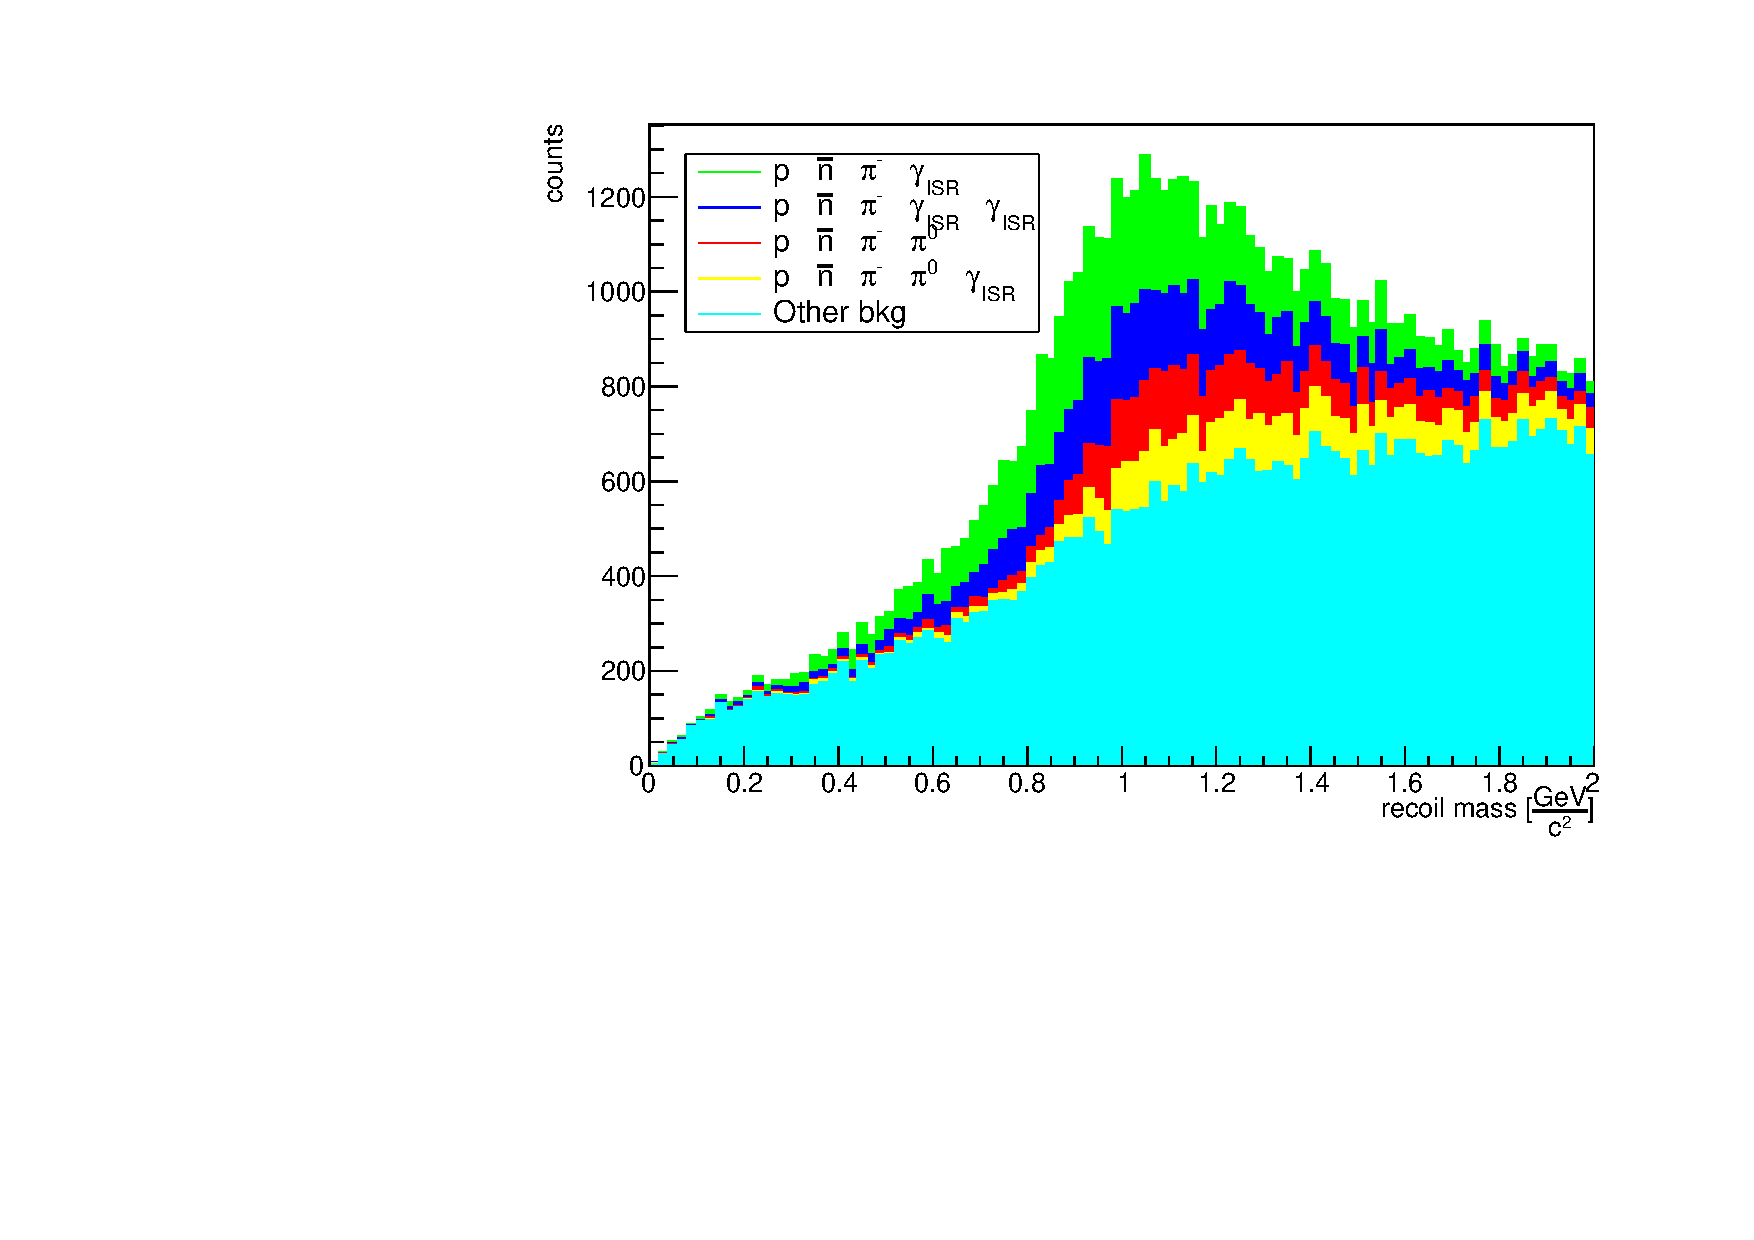
\includegraphics[width=0.8\textwidth]{nbar_cocktail/images/recoilM_qqbar_comps_isr_010}
    \caption{$p, \pi^-$ recoil mass distribution in $q\bar{q}$ Monte Carlo cocktail, displaying each stacked component contribution, ISR case. Green: $\pi^- \bar{n} p \gamma_{ISR}$ channel. Blue: $\pi^- \bar{n} p \gamma_{ISR}$ channel. Red: $\pi^0 \pi^- \bar{n} p$. Yellow: $\pi^0 \pi^- \bar{n} p \gamma_{ISR}$ channel. Cyan: other channels. $\alpha<$ 10 rad cut is applied.}
    \label{fig:mRecComps_isr_010_qqbar}
\end{figure}

No discernible contributions can be observed, as each channel contributes uniformly across the recoil mass distribution, both inside and outside the signal region [0.8, 1.2] GeV. The obtained $\bar{n}$ candidates reconstructed cluster variables are shown in Fig.\ref{fig:clus_vars_nog_qqbar}. 
 \begin{figure}[h]
    \centering
    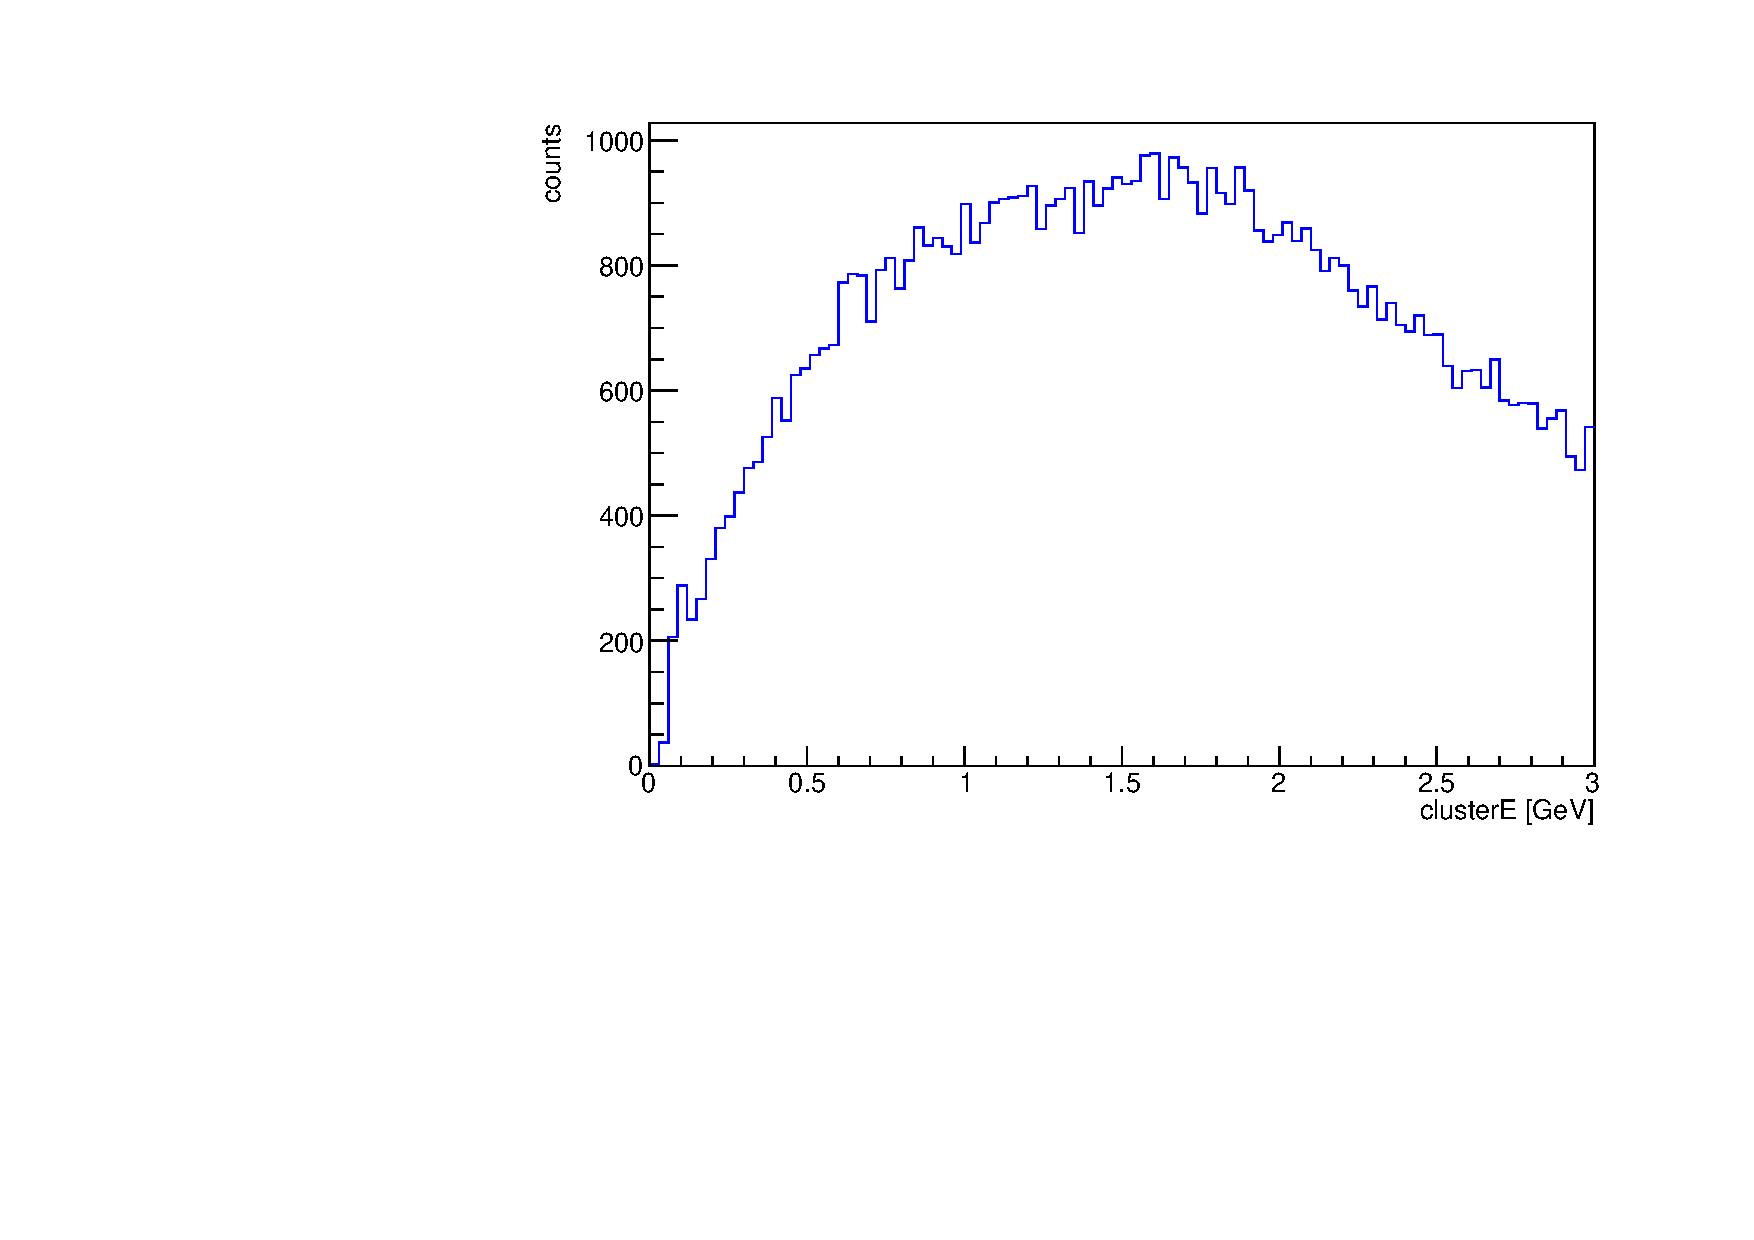
\includegraphics[width=0.49\textwidth]{nbar_cocktail/images/clusterE_isr_qqbar.pdf}
    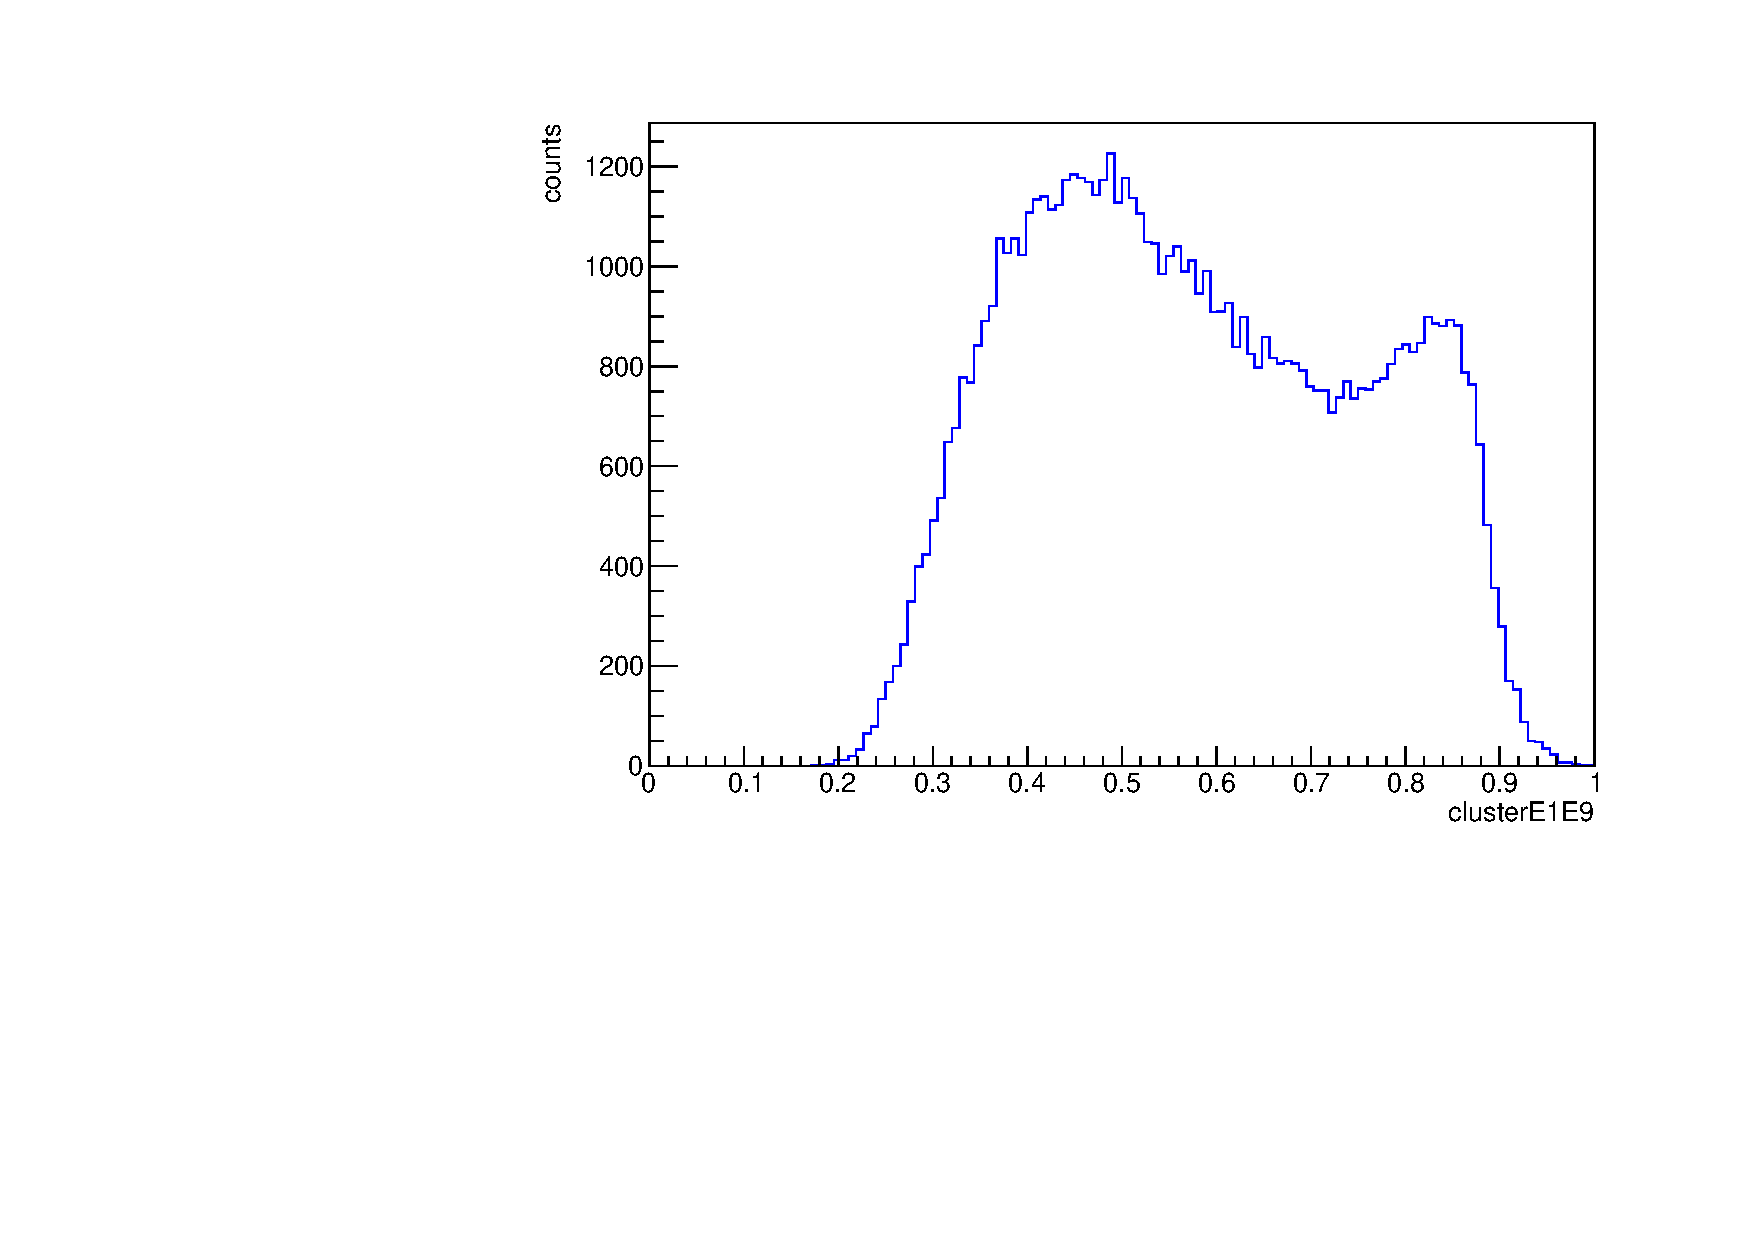
\includegraphics[width=0.49\textwidth]{nbar_cocktail/images/clusterE1E9_isr_qqbar.pdf}
    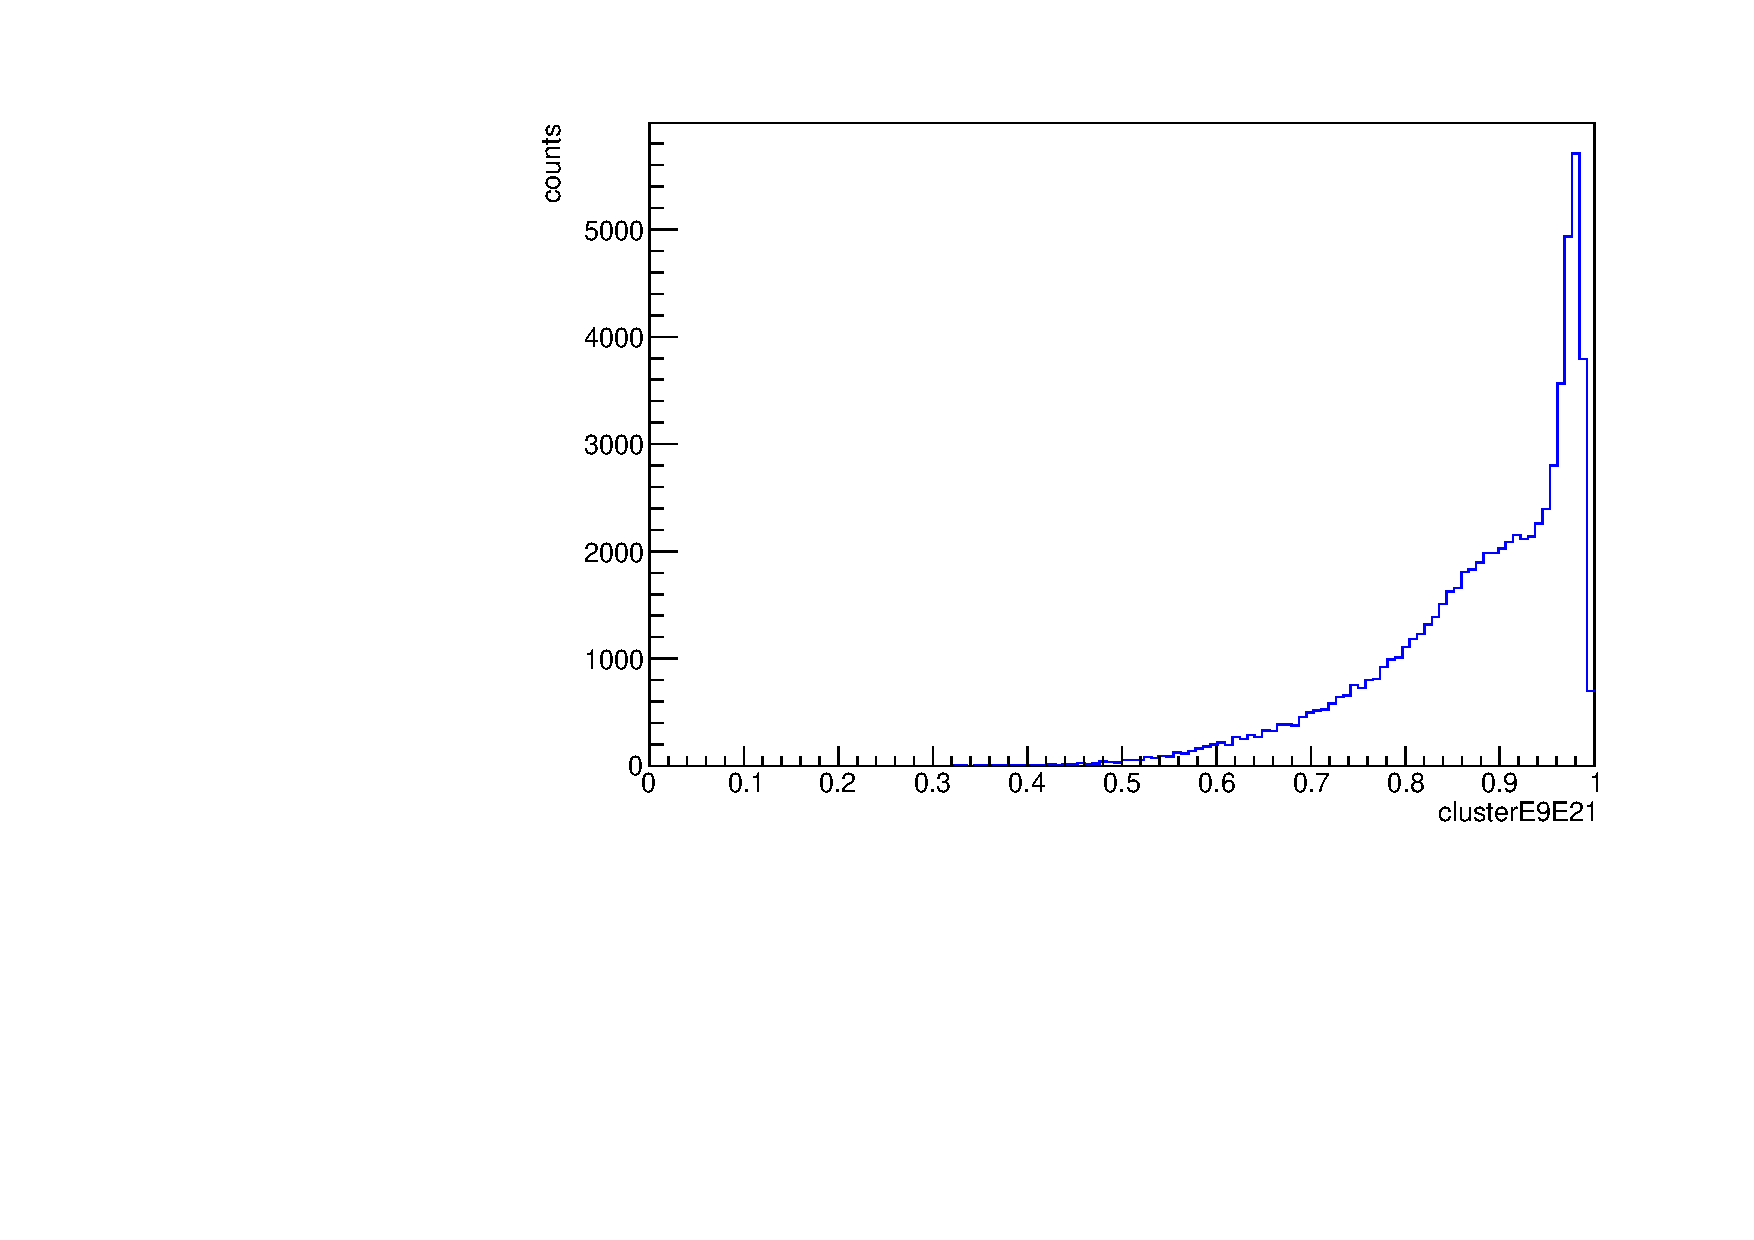
\includegraphics[width=0.49\textwidth]{nbar_cocktail/images/clusterE9E21_isr_qqbar.pdf}
    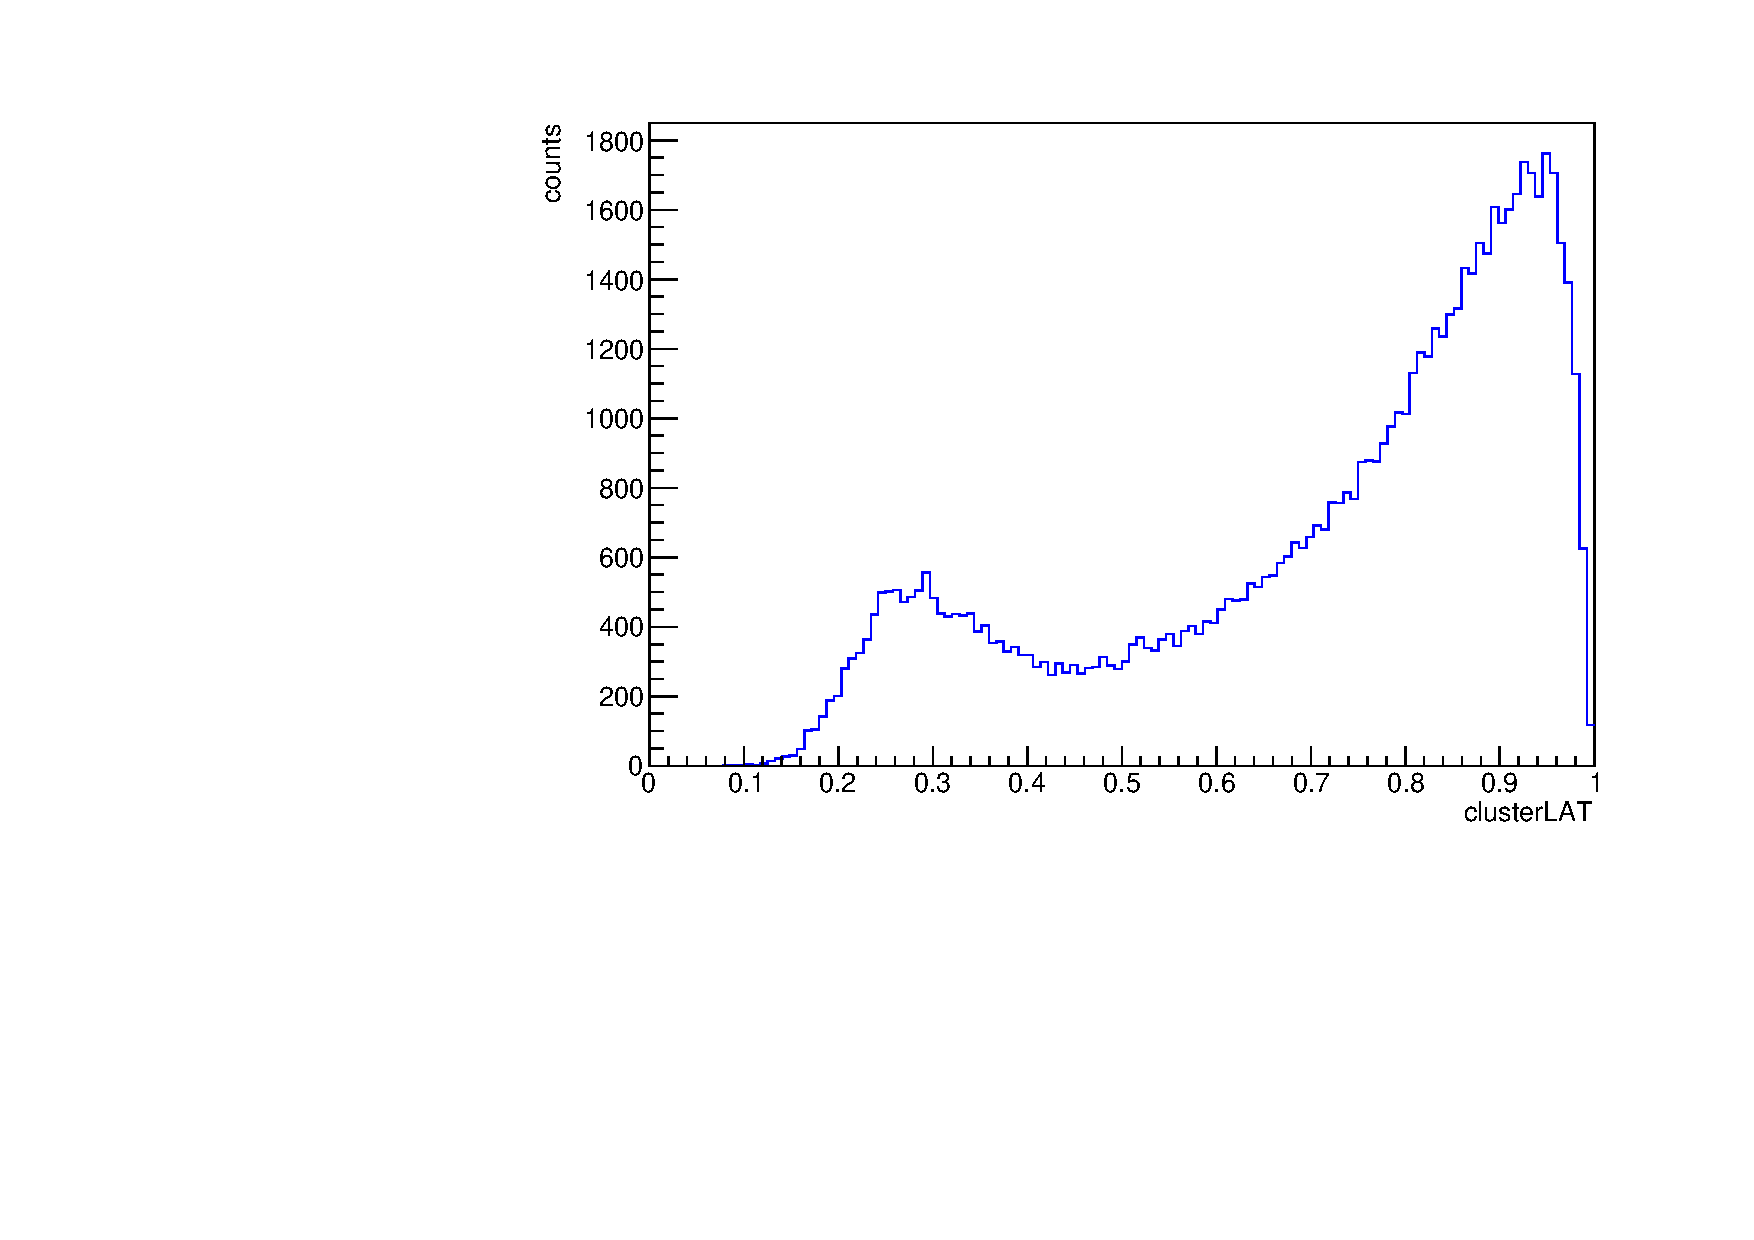
\includegraphics[width=0.49\textwidth]{nbar_cocktail/images/clusterLAT_isr_qqbar.pdf}
    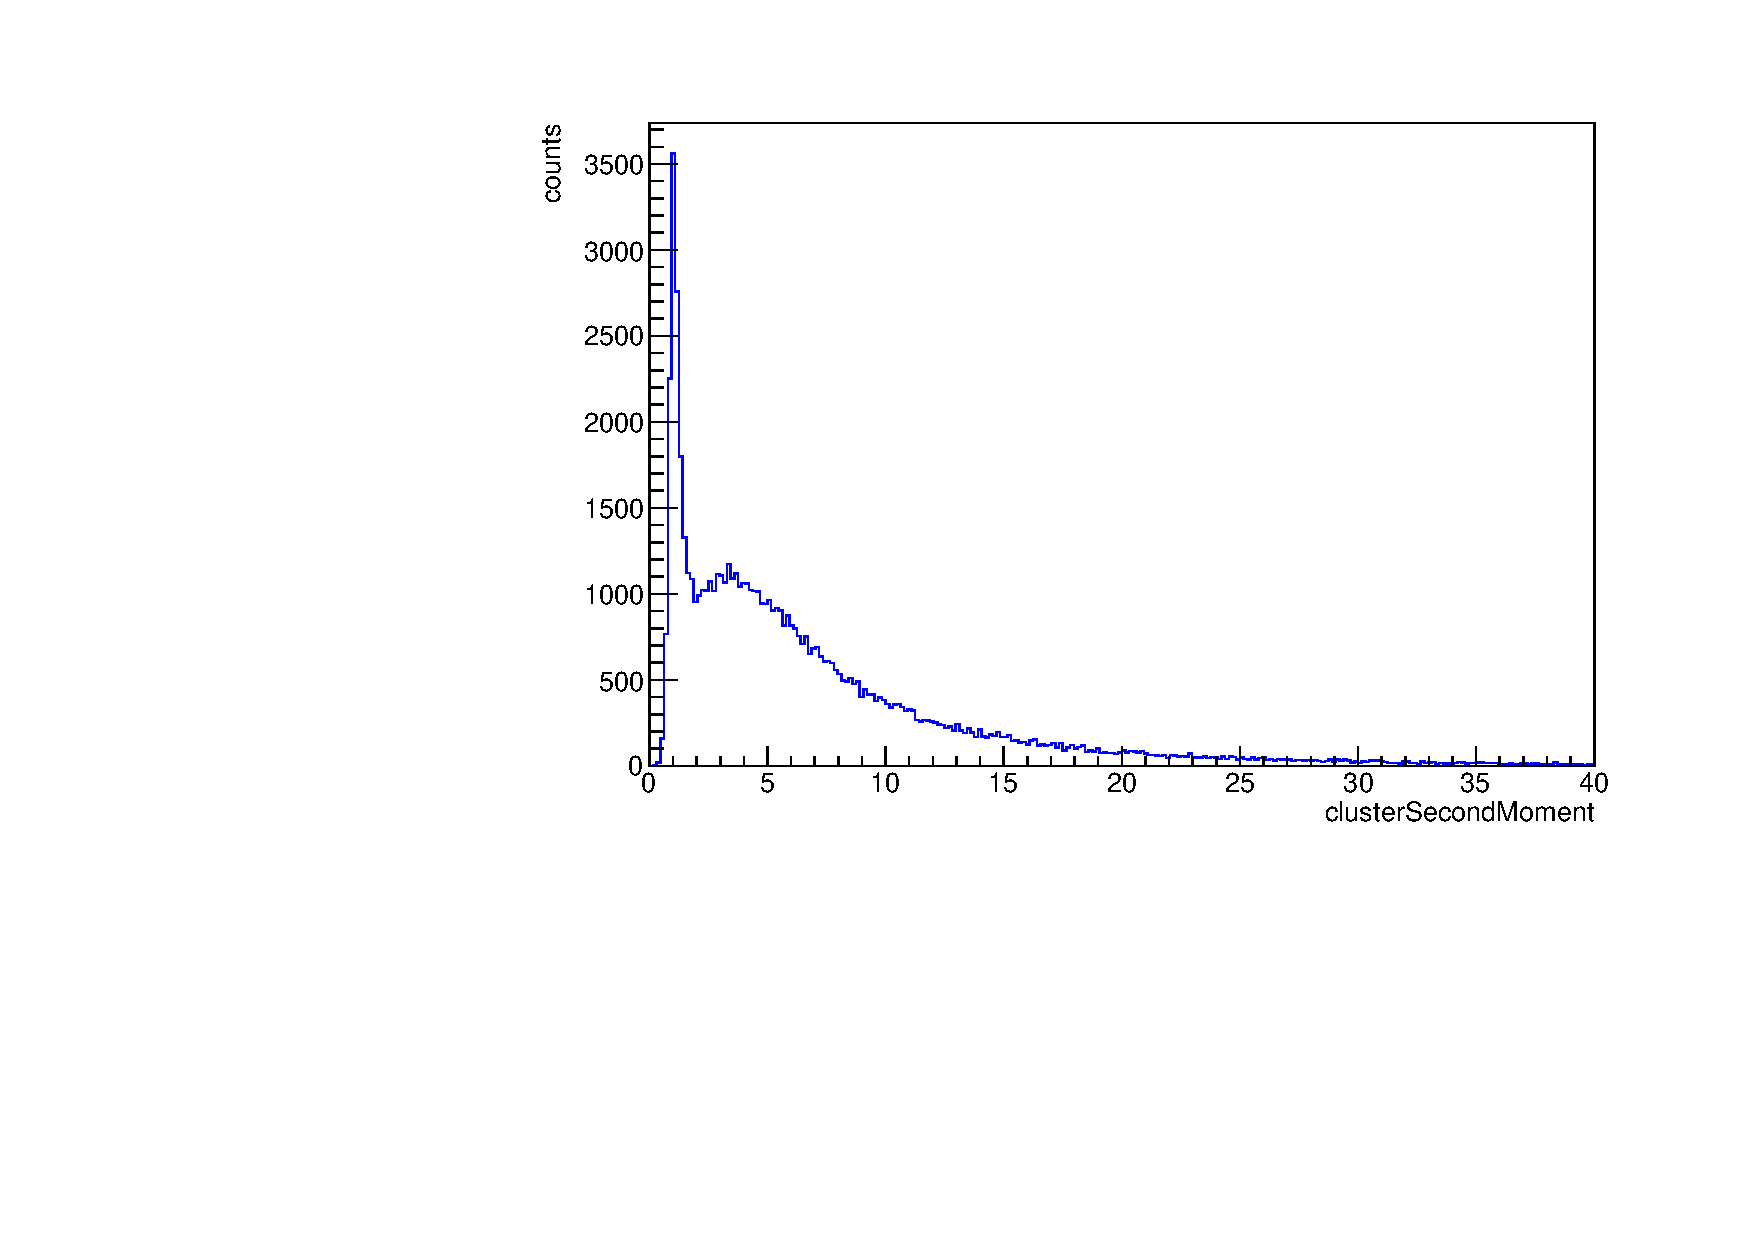
\includegraphics[width=0.49\textwidth]{nbar_cocktail/images/clusterSecondMoment_isr_qqbar.pdf}
    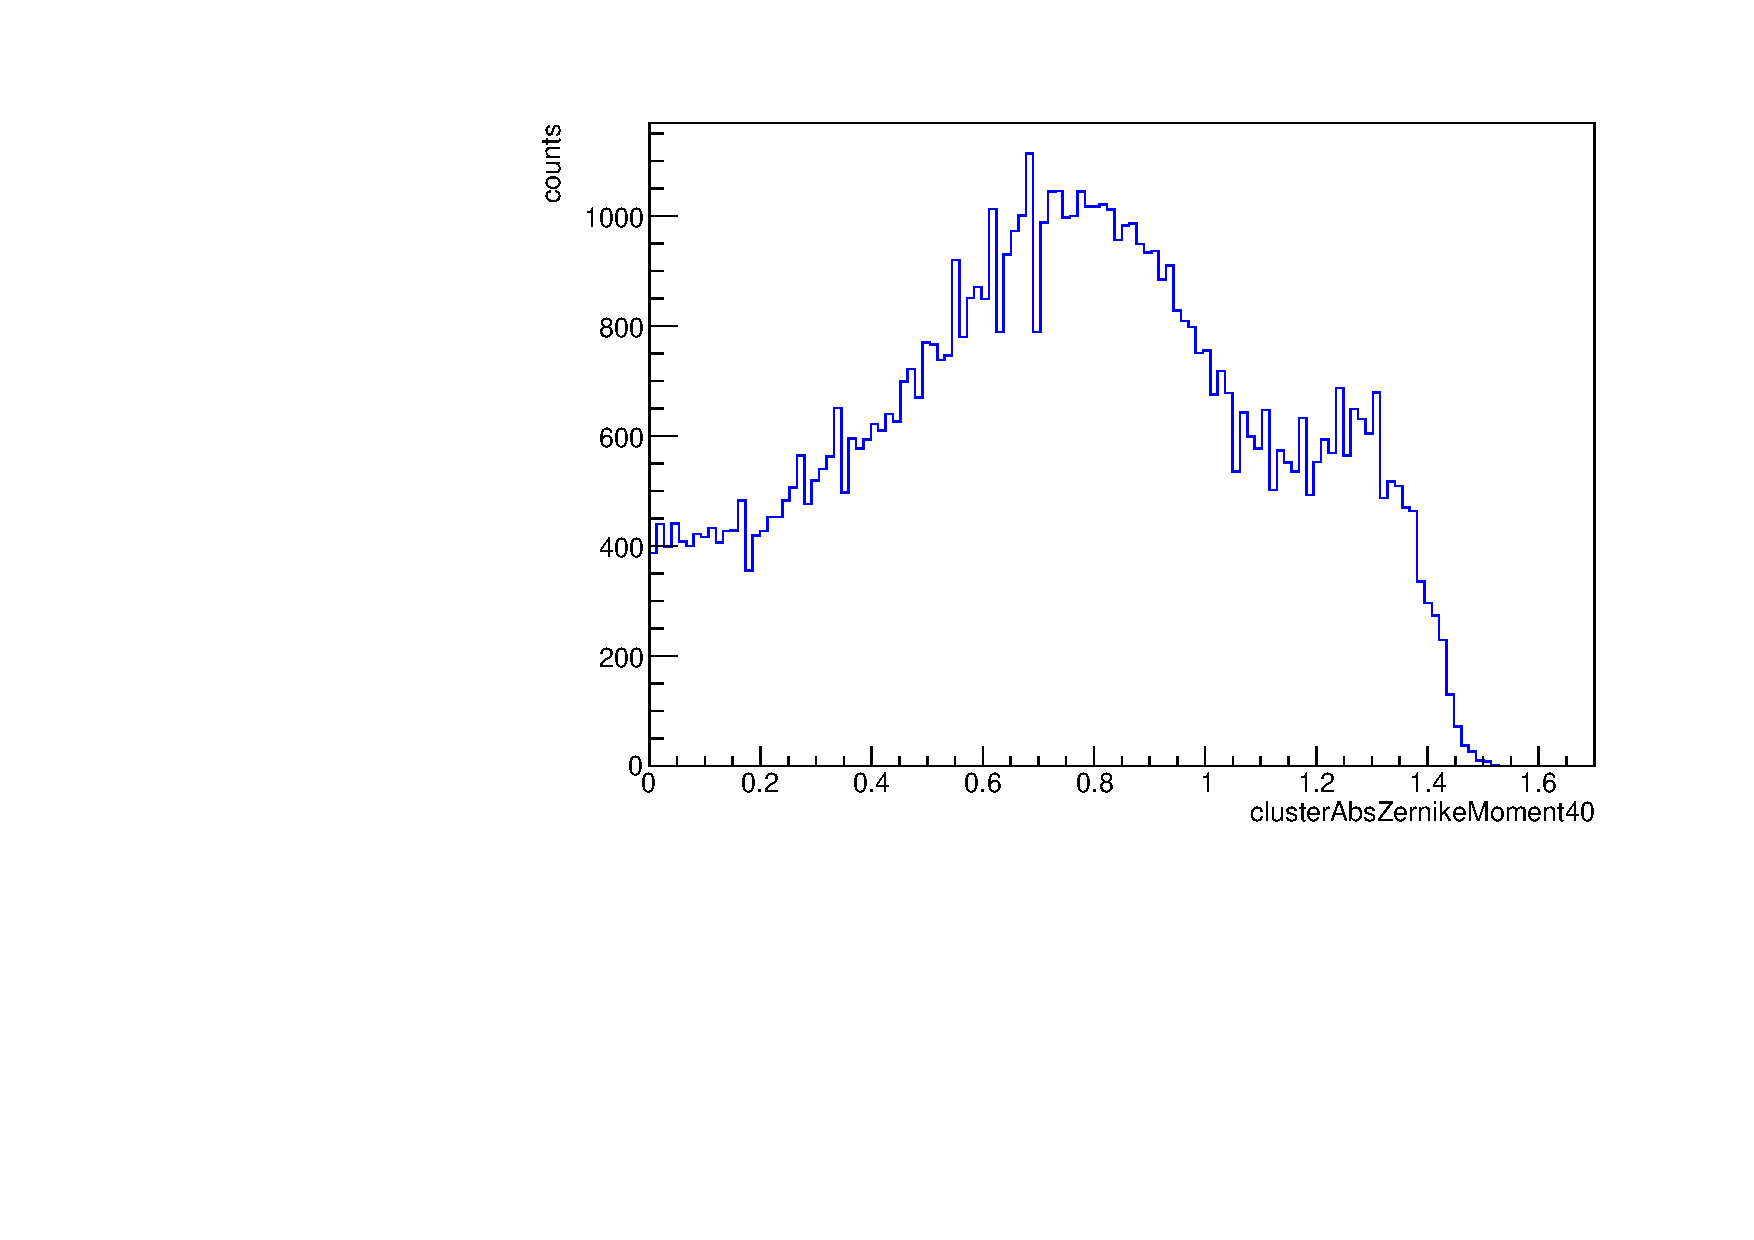
\includegraphics[width=0.49\textwidth]{nbar_cocktail/images/clusterAbsZernikeMoment40_isr_qqbar.pdf}
    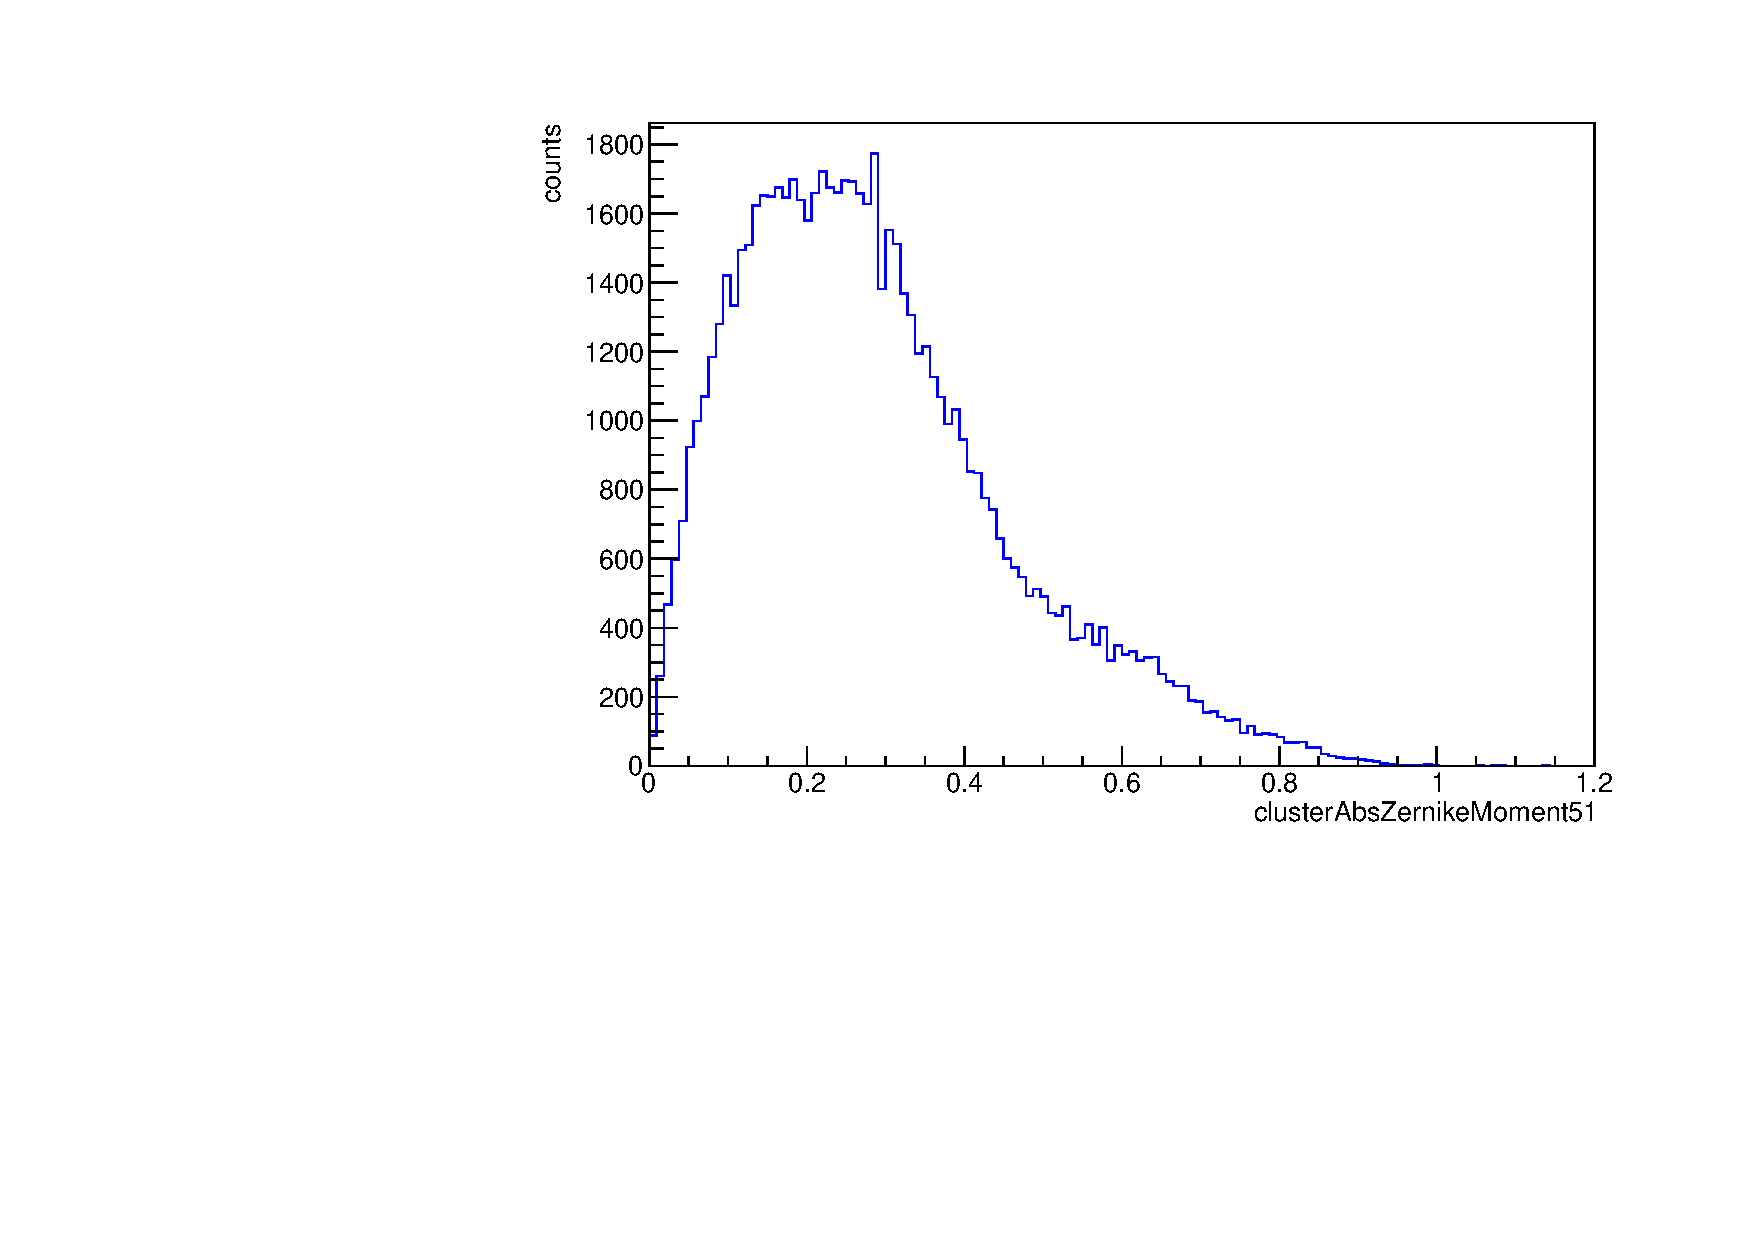
\includegraphics[width=0.49\textwidth]{nbar_cocktail/images/clusterAbsZernikeMoment51_isr_qqbar.pdf}
    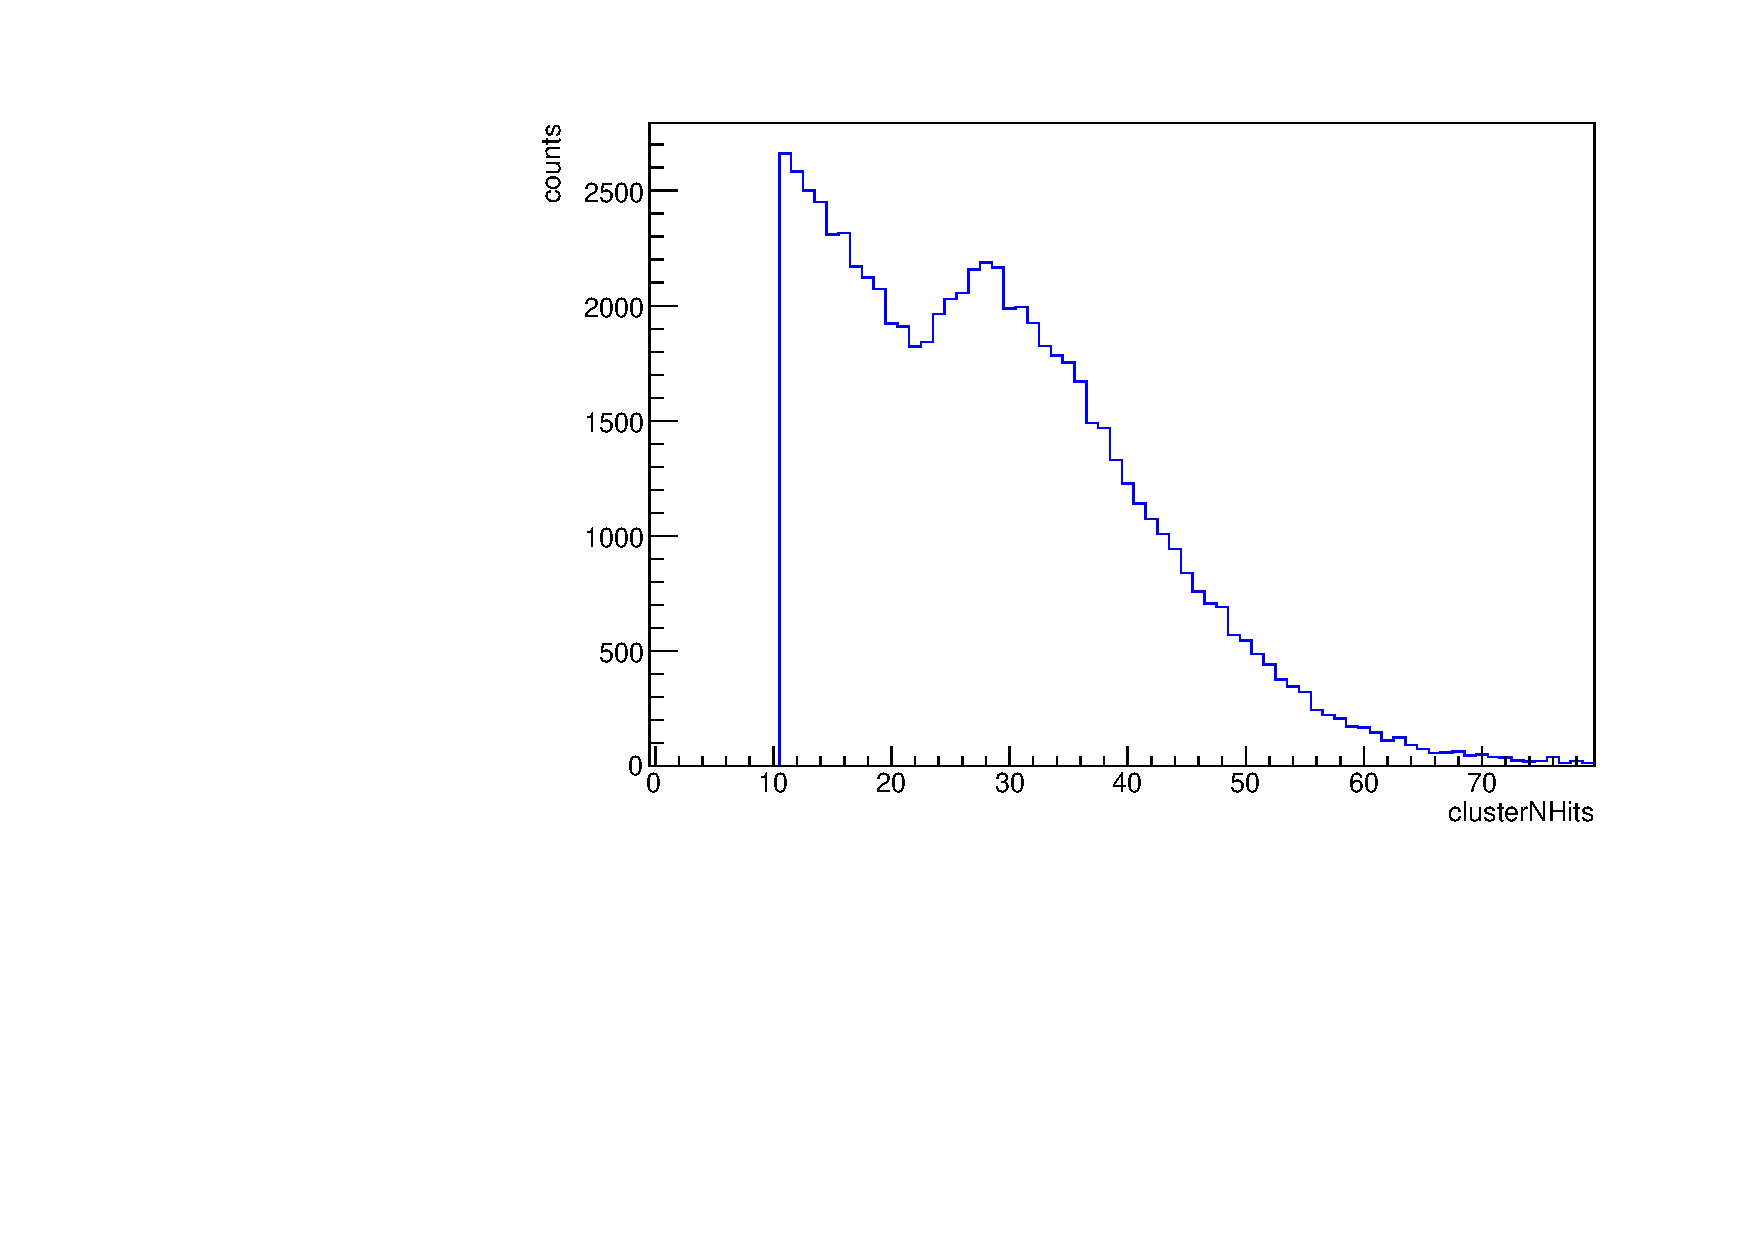
\includegraphics[width=0.49\textwidth]{nbar_cocktail/images/clusterNHits_isr_qqbar.pdf}
     \caption{Reconstructed cluster variables distribution for $\bar{n}$ candidates in the for the recoil mass region [0, 2] GeV, in ISR case. q$\bar{q}$ cocktail }
     \label{fig:clus_vars_isr_qqbar}
\end{figure}
$\\$
Since substantial background appears to the right of the signal region -suggesting that particles are missing from the recoil reconstruction- the sideband regions are redefined, for the ISR case, as follows:
\begin{itemize}
\item Signal region: [0.8, 1.4] GeV;
\item Sidebands regions: [0.2, 0.8] U [1.4, 2.0]  GeV;
\item $k = \frac{1.4 - 0.8}{(0.8 - 0.2) + (2.0 - 1.4)} = \frac{1}{2}$.
\end{itemize}

The signal region and sidebands region, in the recoil mass distribution  are shown in Fig.\ref{fig:recMass_sidebands_isr}.
\begin{figure}[H]
    \centering
    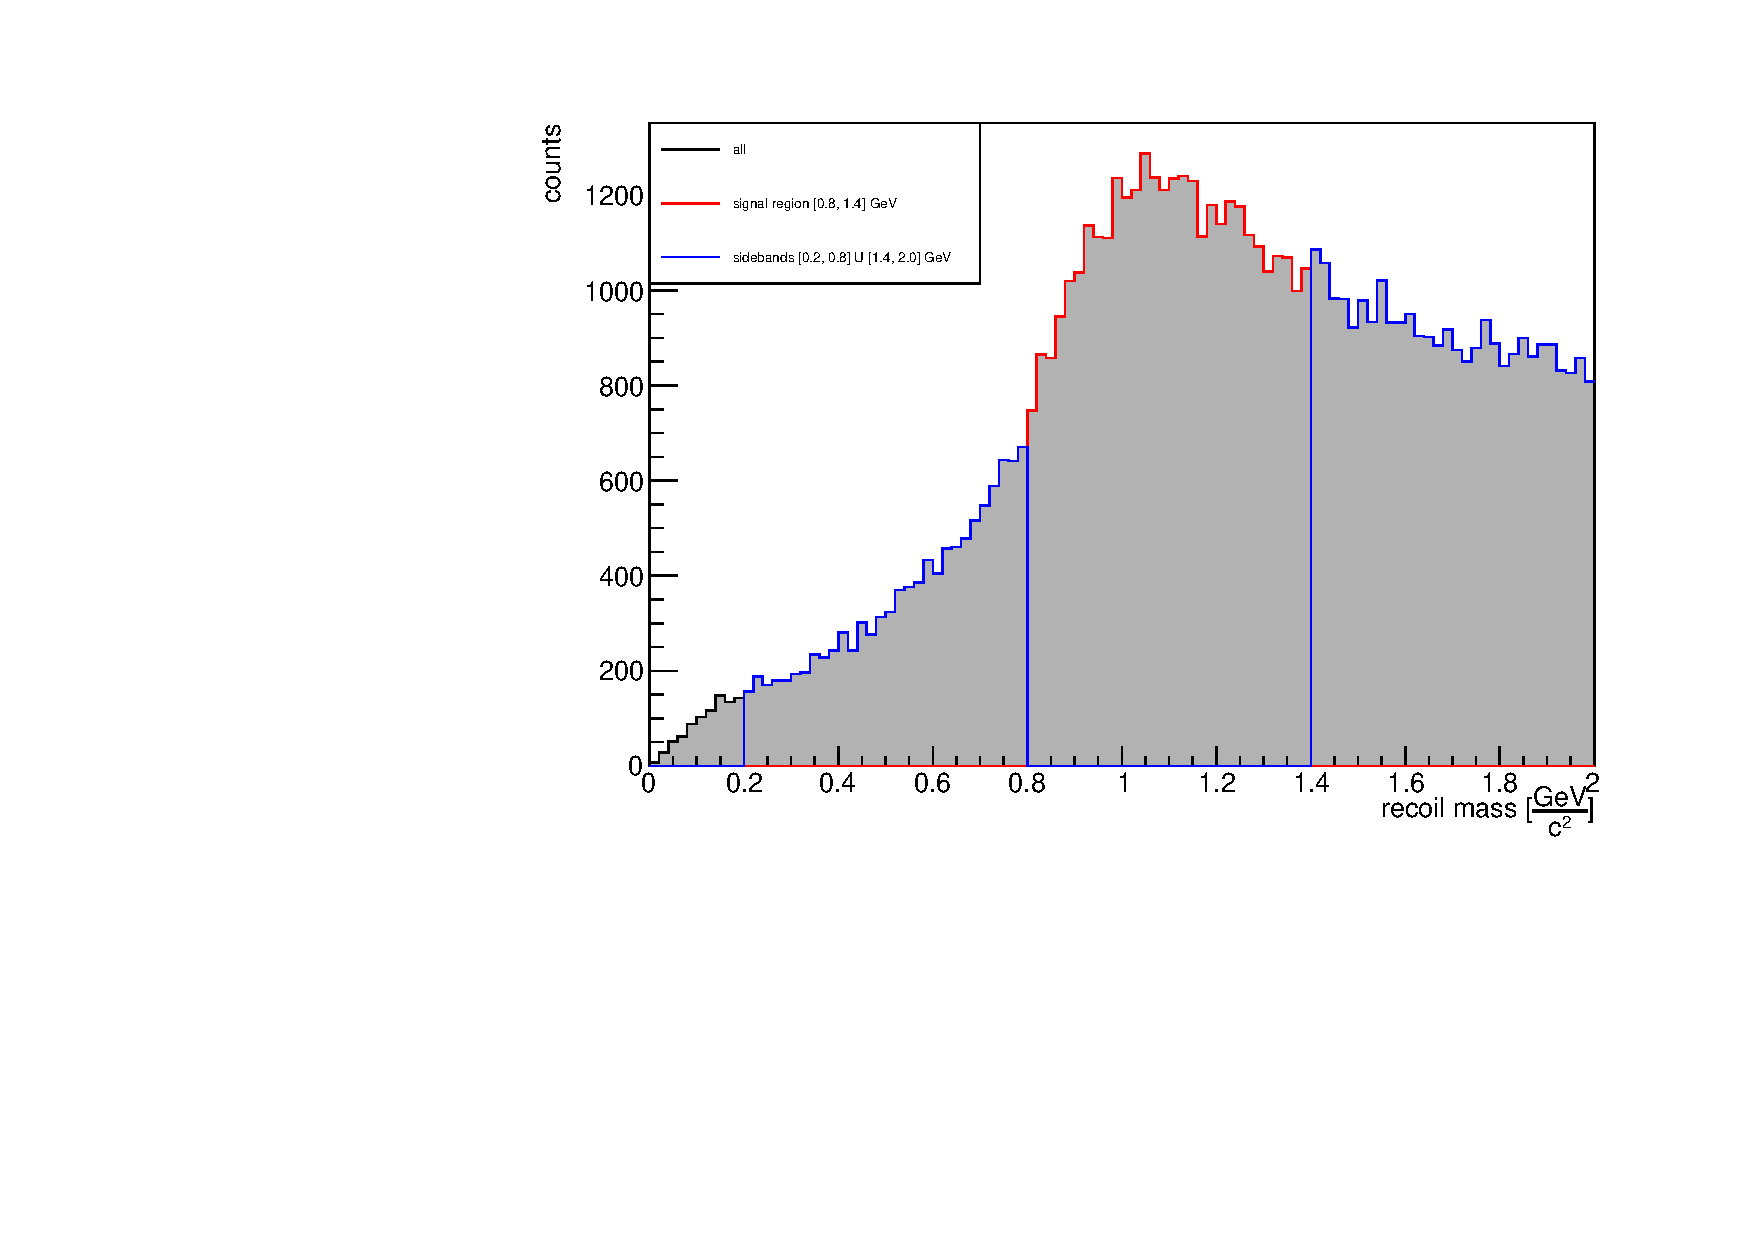
\includegraphics[width=0.6\textwidth]{nbar_cocktail/images/recoil_mass_sidebands_isr}
    \caption{Recoil mass distribution (black), with the signal region (red) and the sidebands regions (blue), in the $q\bar{q}$ Monte Carlo cocktail. ISR case.}
    \label{fig:recMass_sidebands_isr}
\end{figure}

The obtained cluster variables contribution is shown in Fig.\ref{fig:clus_vars_sidebands_pre_isr}.
 \begin{figure}[h]
    \centering
    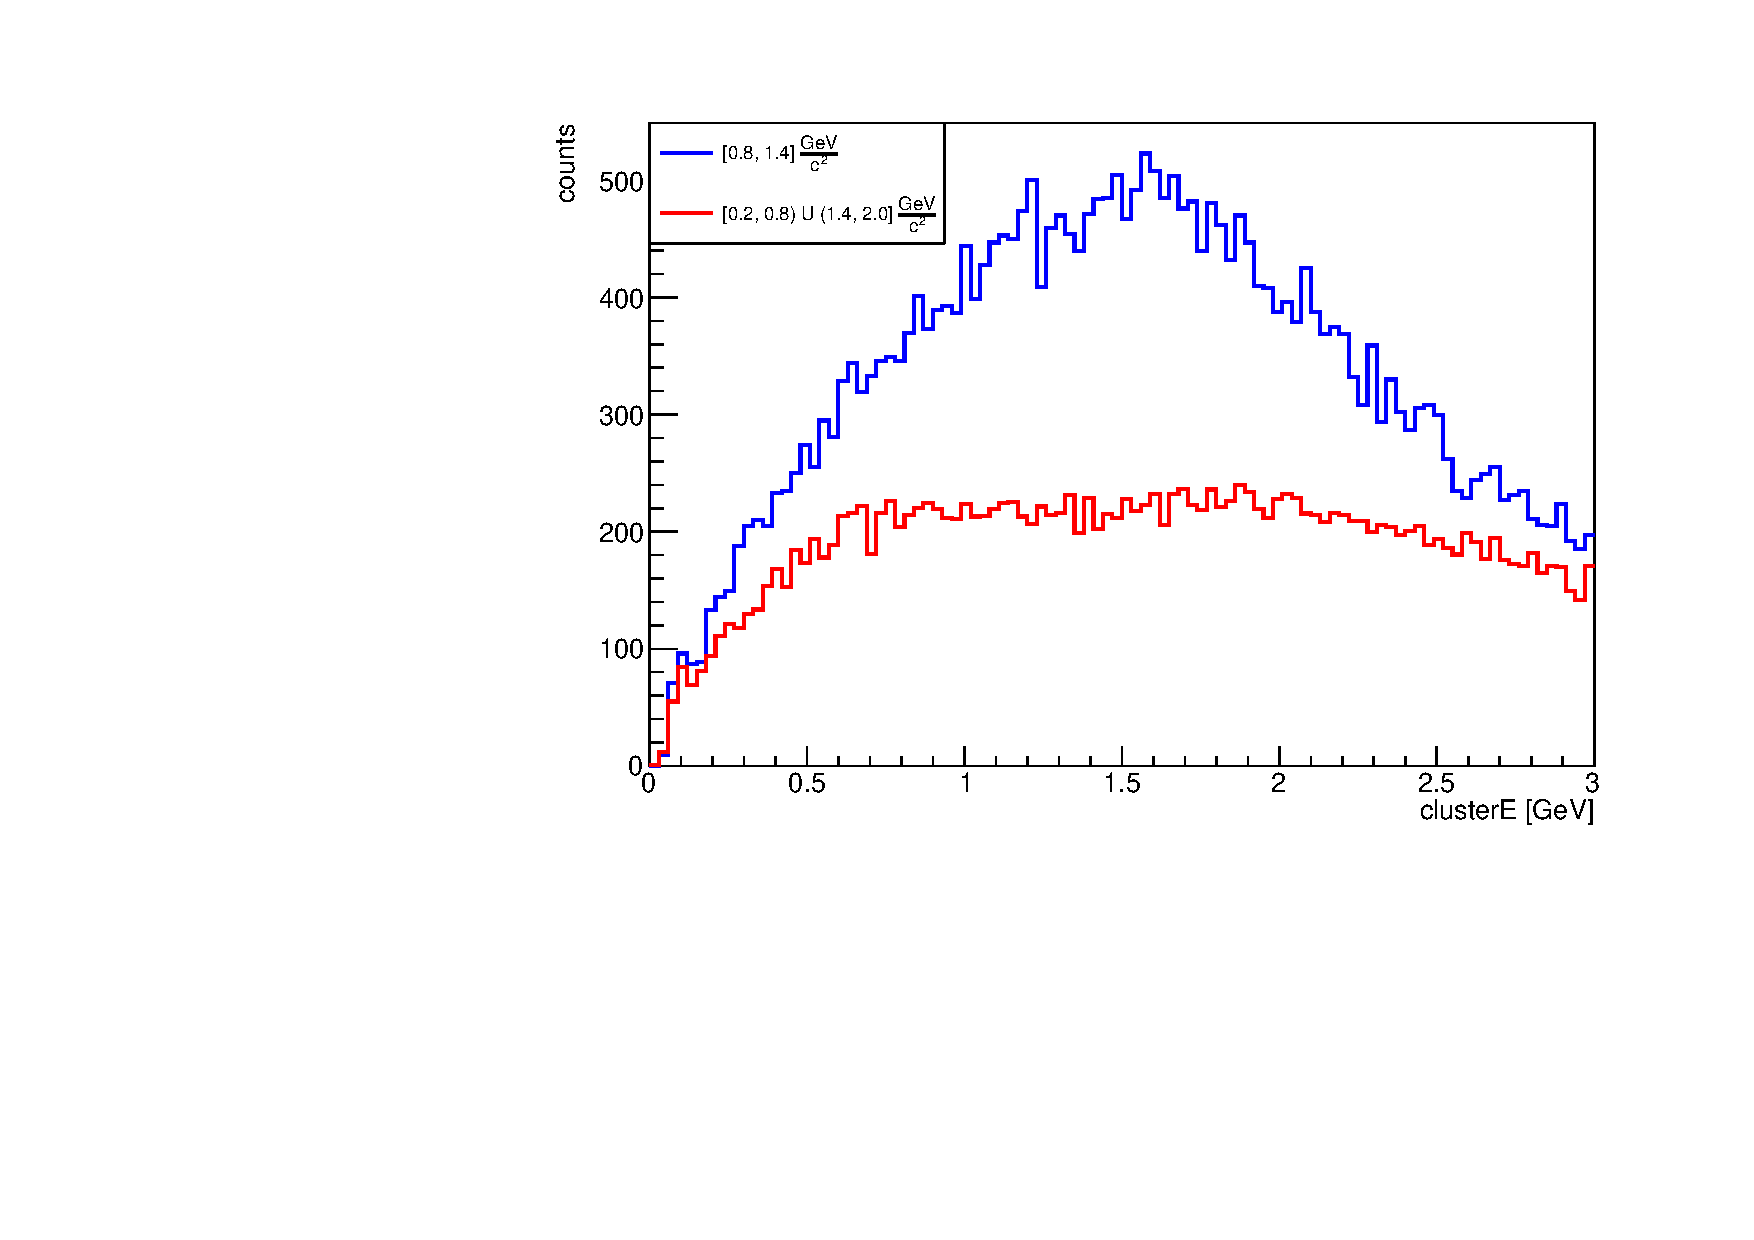
\includegraphics[width=0.49\textwidth]{nbar_cocktail/images/sidebands_clusterE_isr.pdf}
    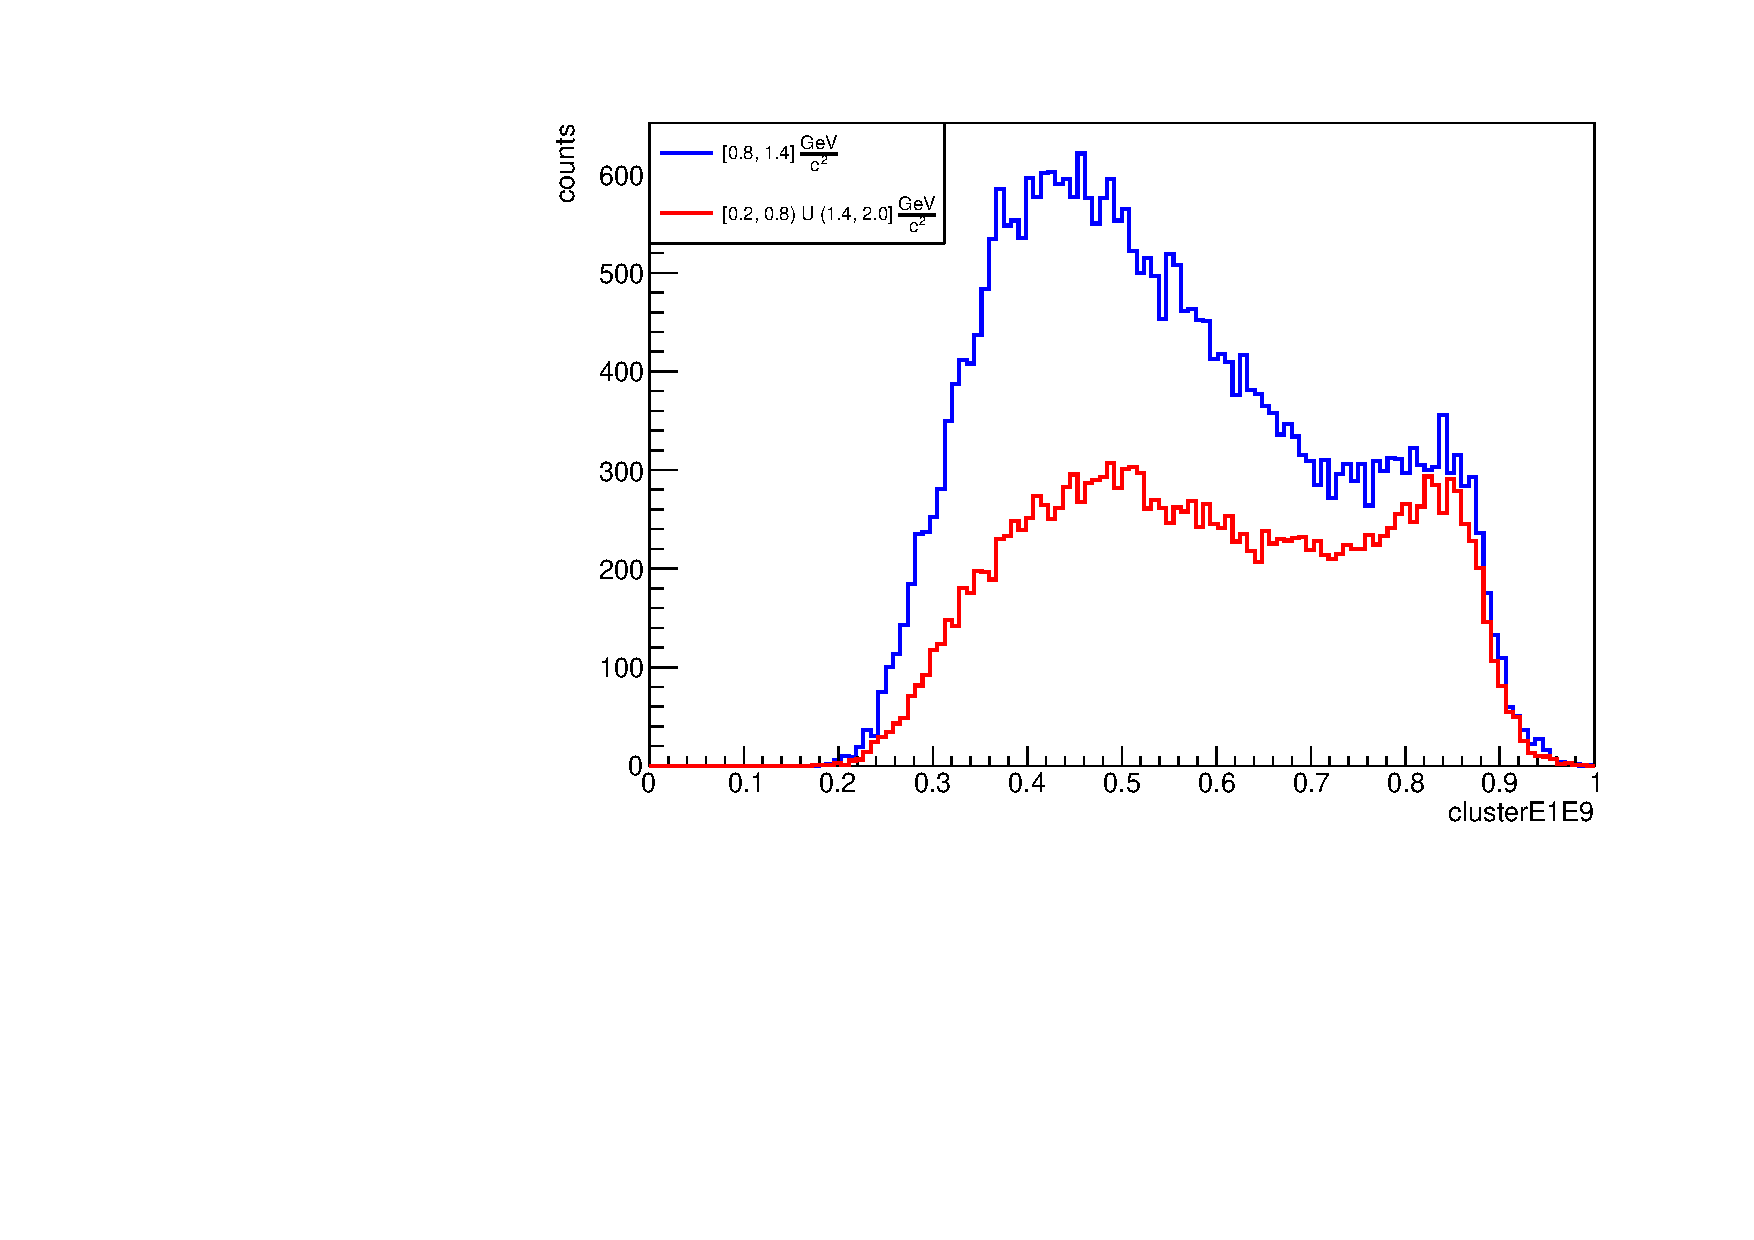
\includegraphics[width=0.49\textwidth]{nbar_cocktail/images/sidebands_clusterE1E9_isr.pdf}
    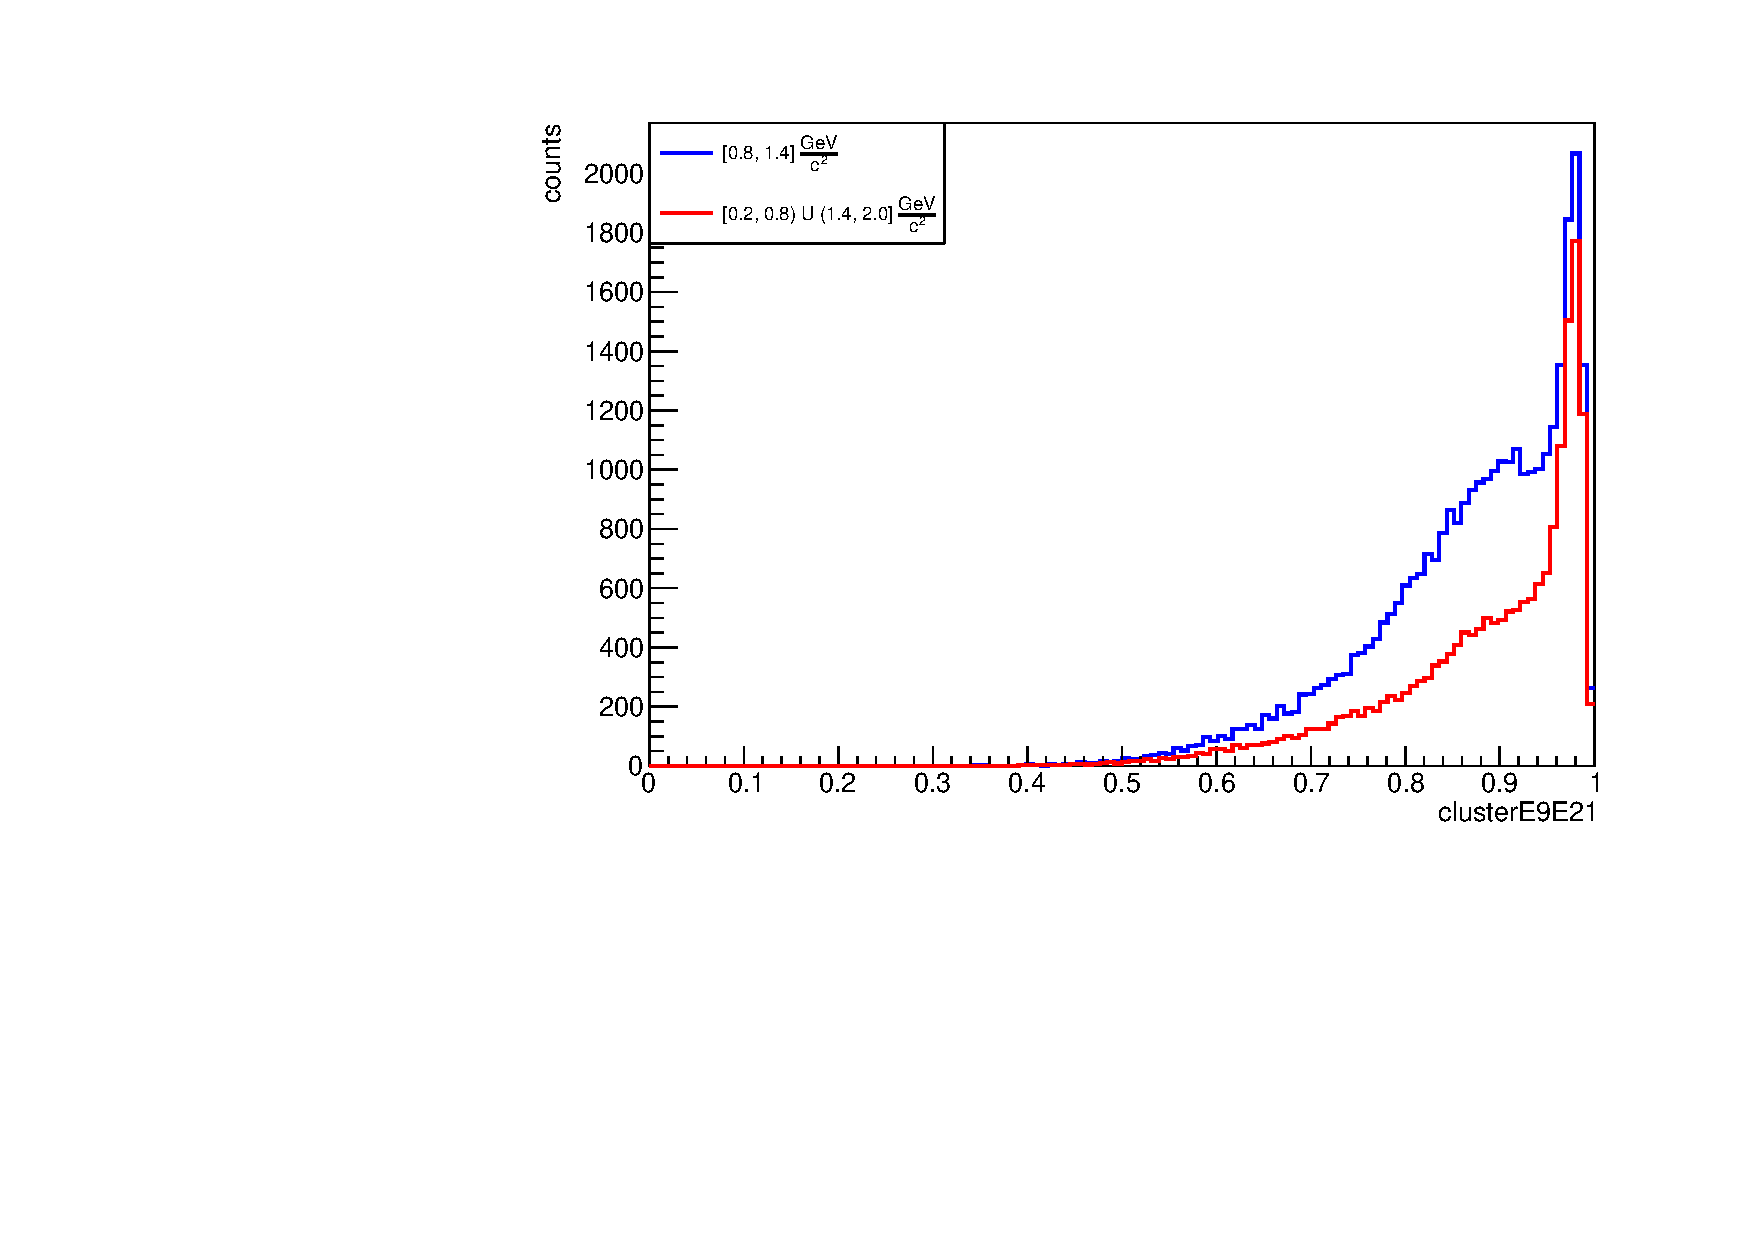
\includegraphics[width=0.49\textwidth]{nbar_cocktail/images/sidebands_clusterE9E21_isr.pdf}
    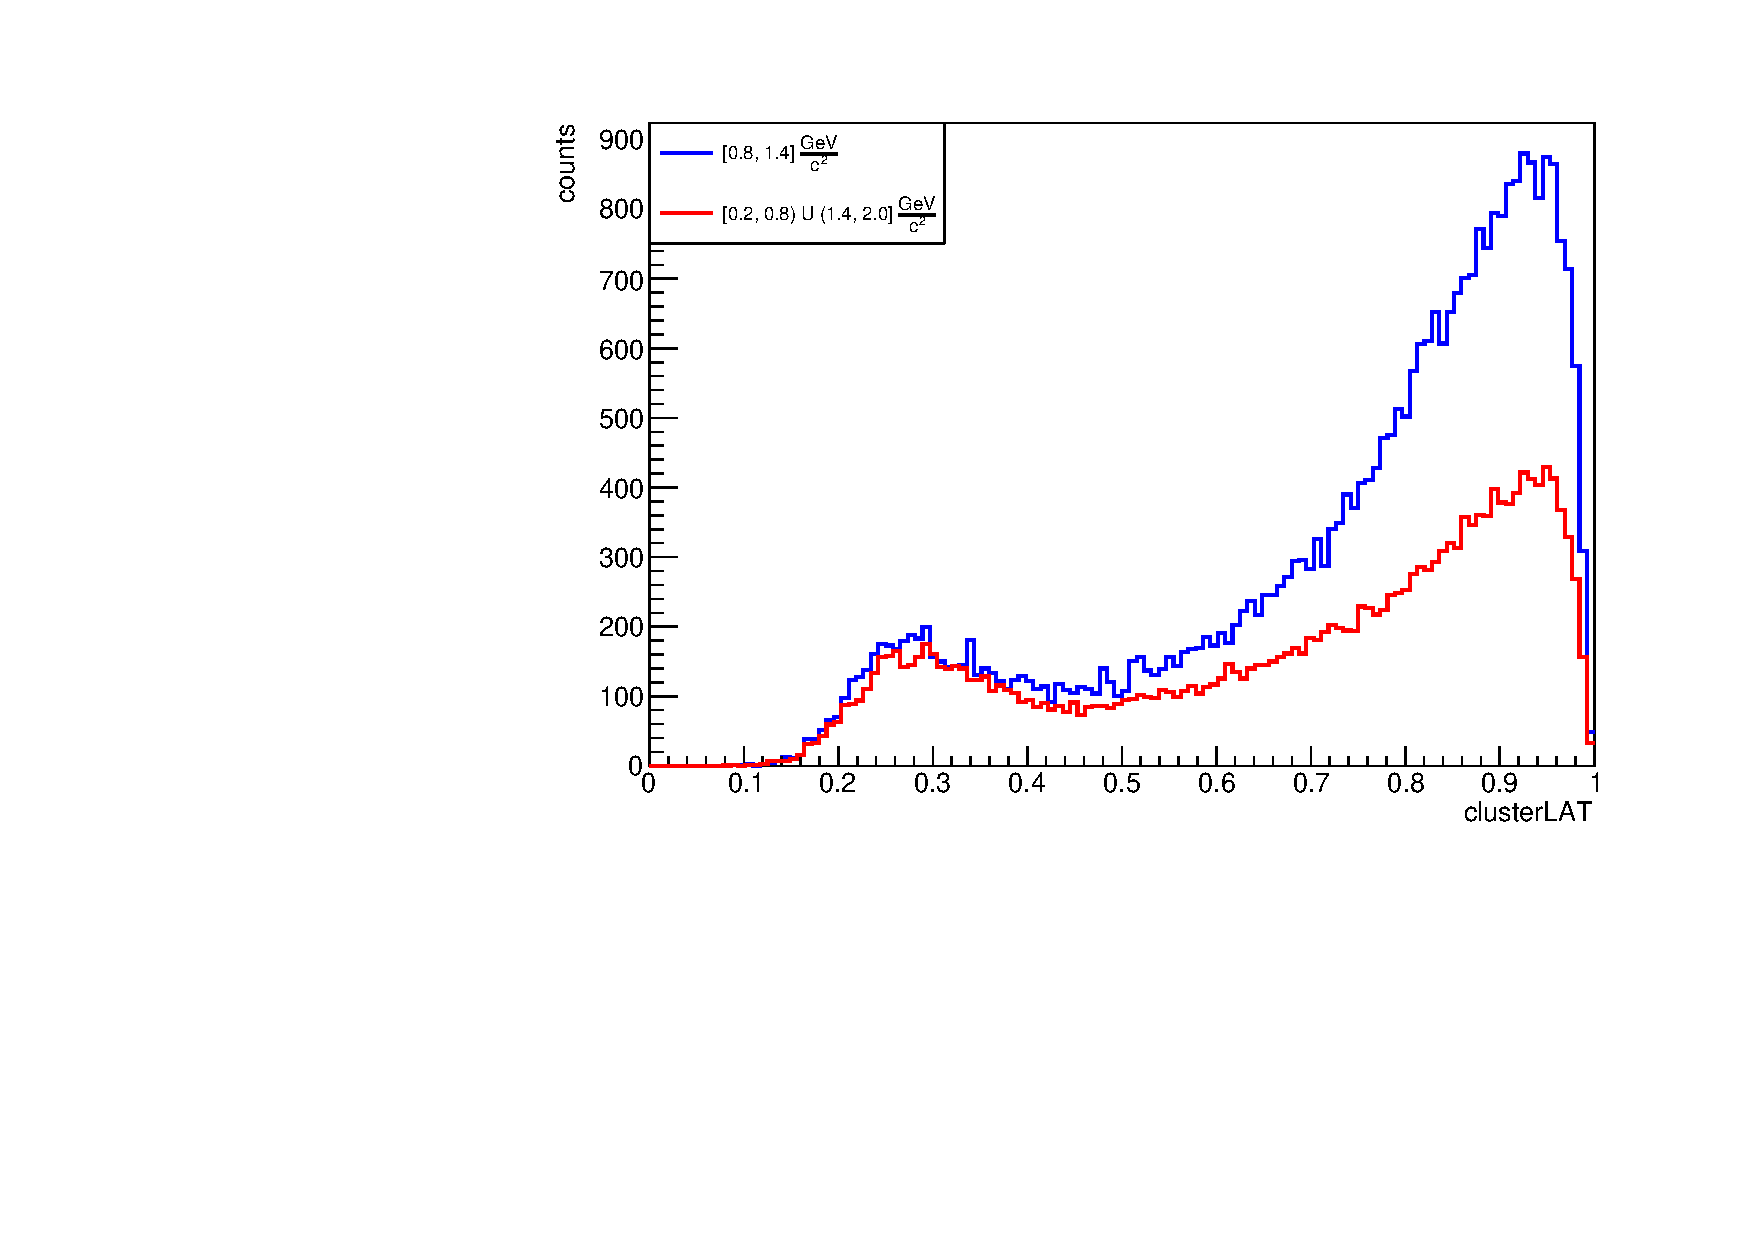
\includegraphics[width=0.49\textwidth]{nbar_cocktail/images/sidebands_clusterLAT_isr.pdf}
    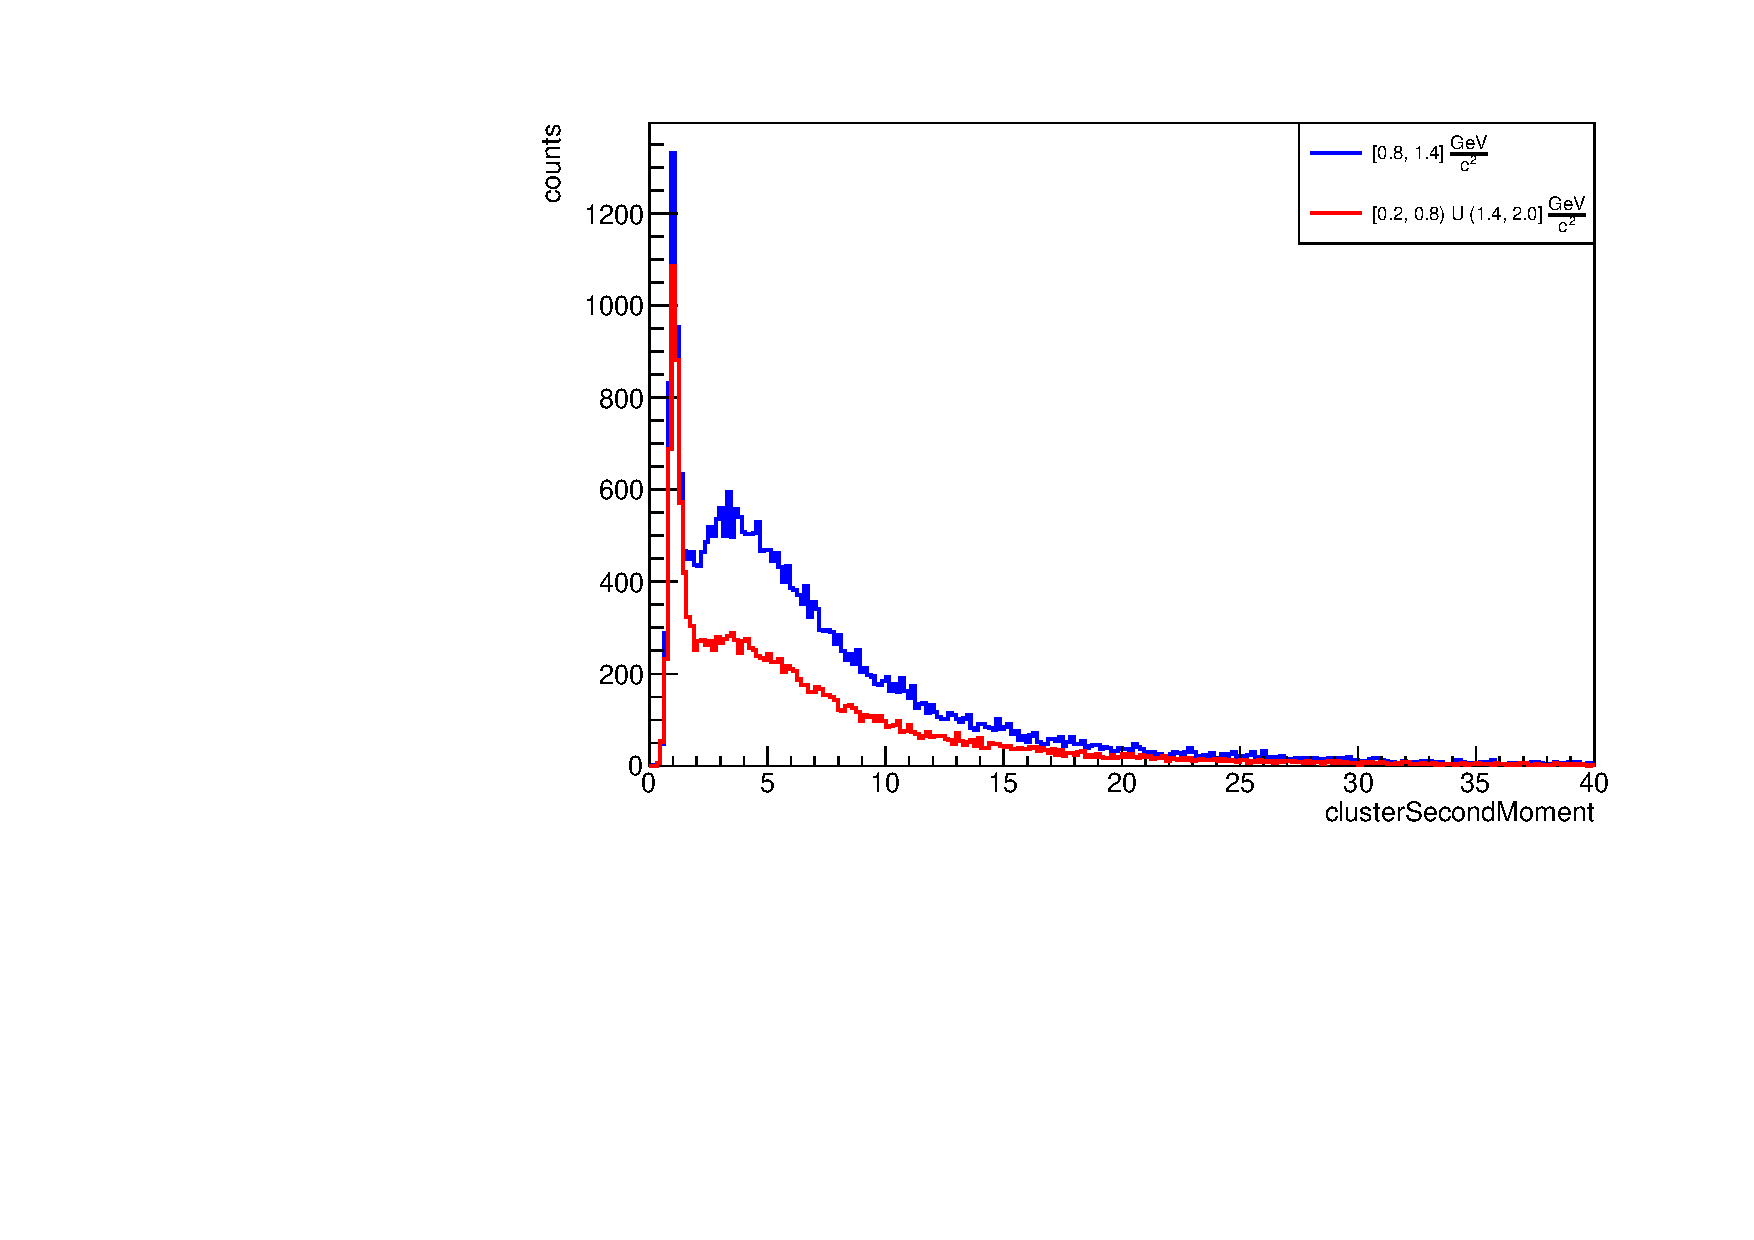
\includegraphics[width=0.49\textwidth]{nbar_cocktail/images/sidebands_clusterSecondMoment_isr.pdf}
    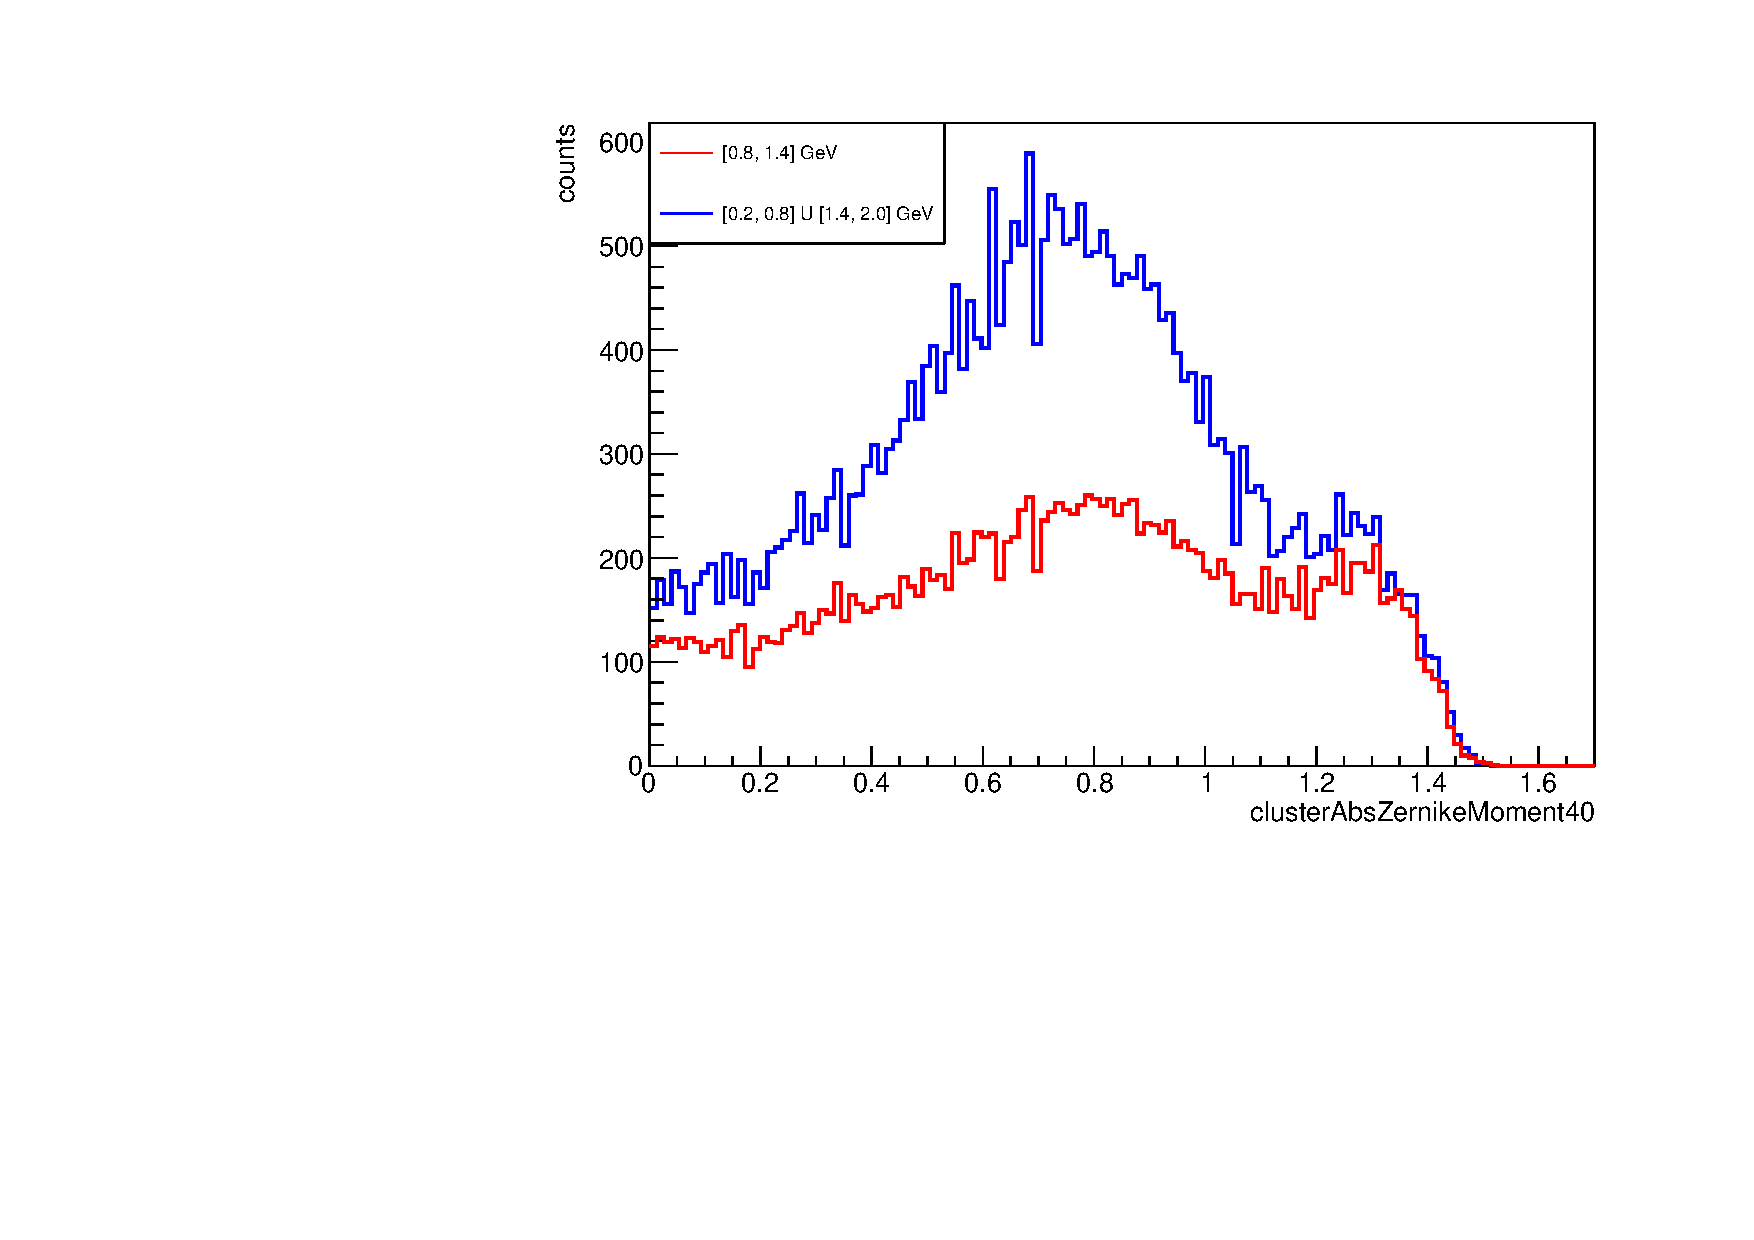
\includegraphics[width=0.49\textwidth]{nbar_cocktail/images/sidebands_clusterAbsZernikeMoment40_isr.pdf}
    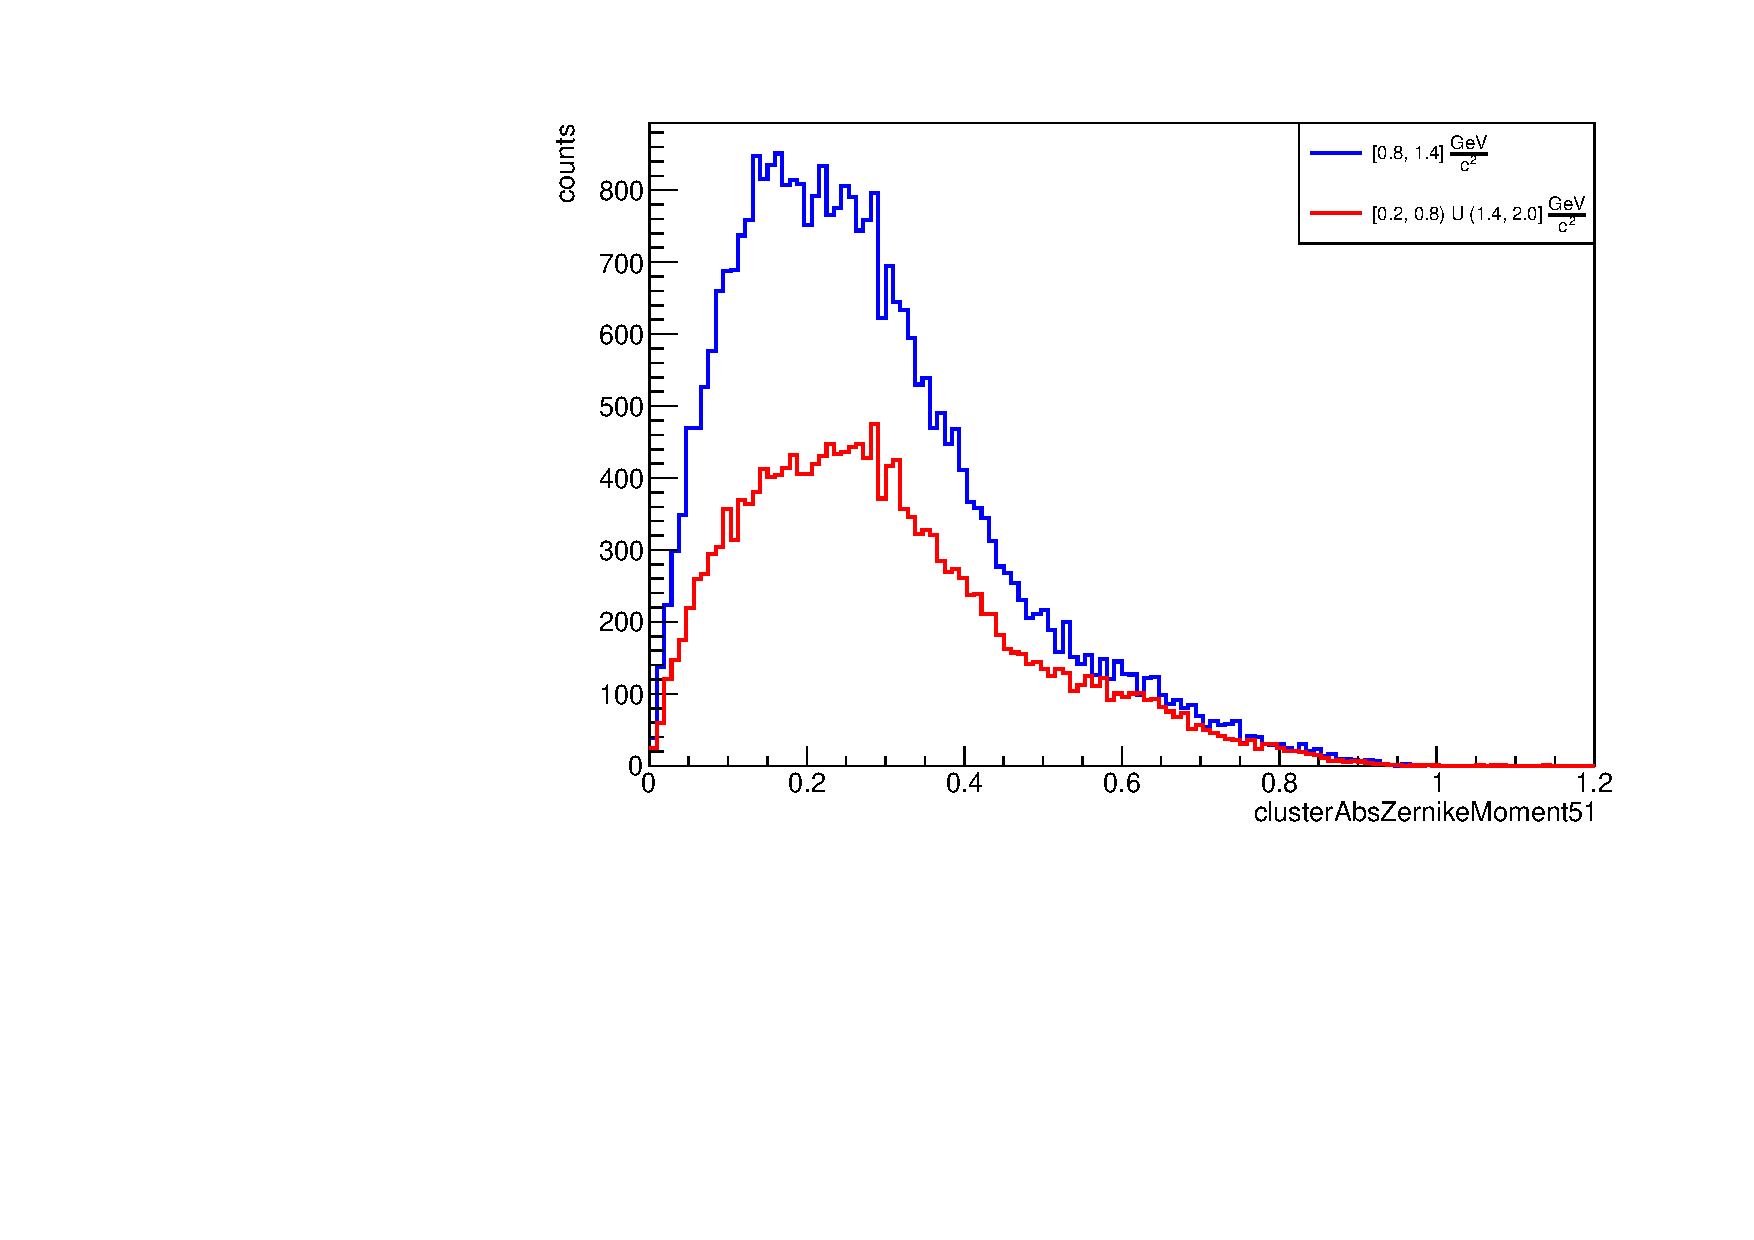
\includegraphics[width=0.49\textwidth]{nbar_cocktail/images/sidebands_clusterAbsZernikeMoment51_isr.pdf}
    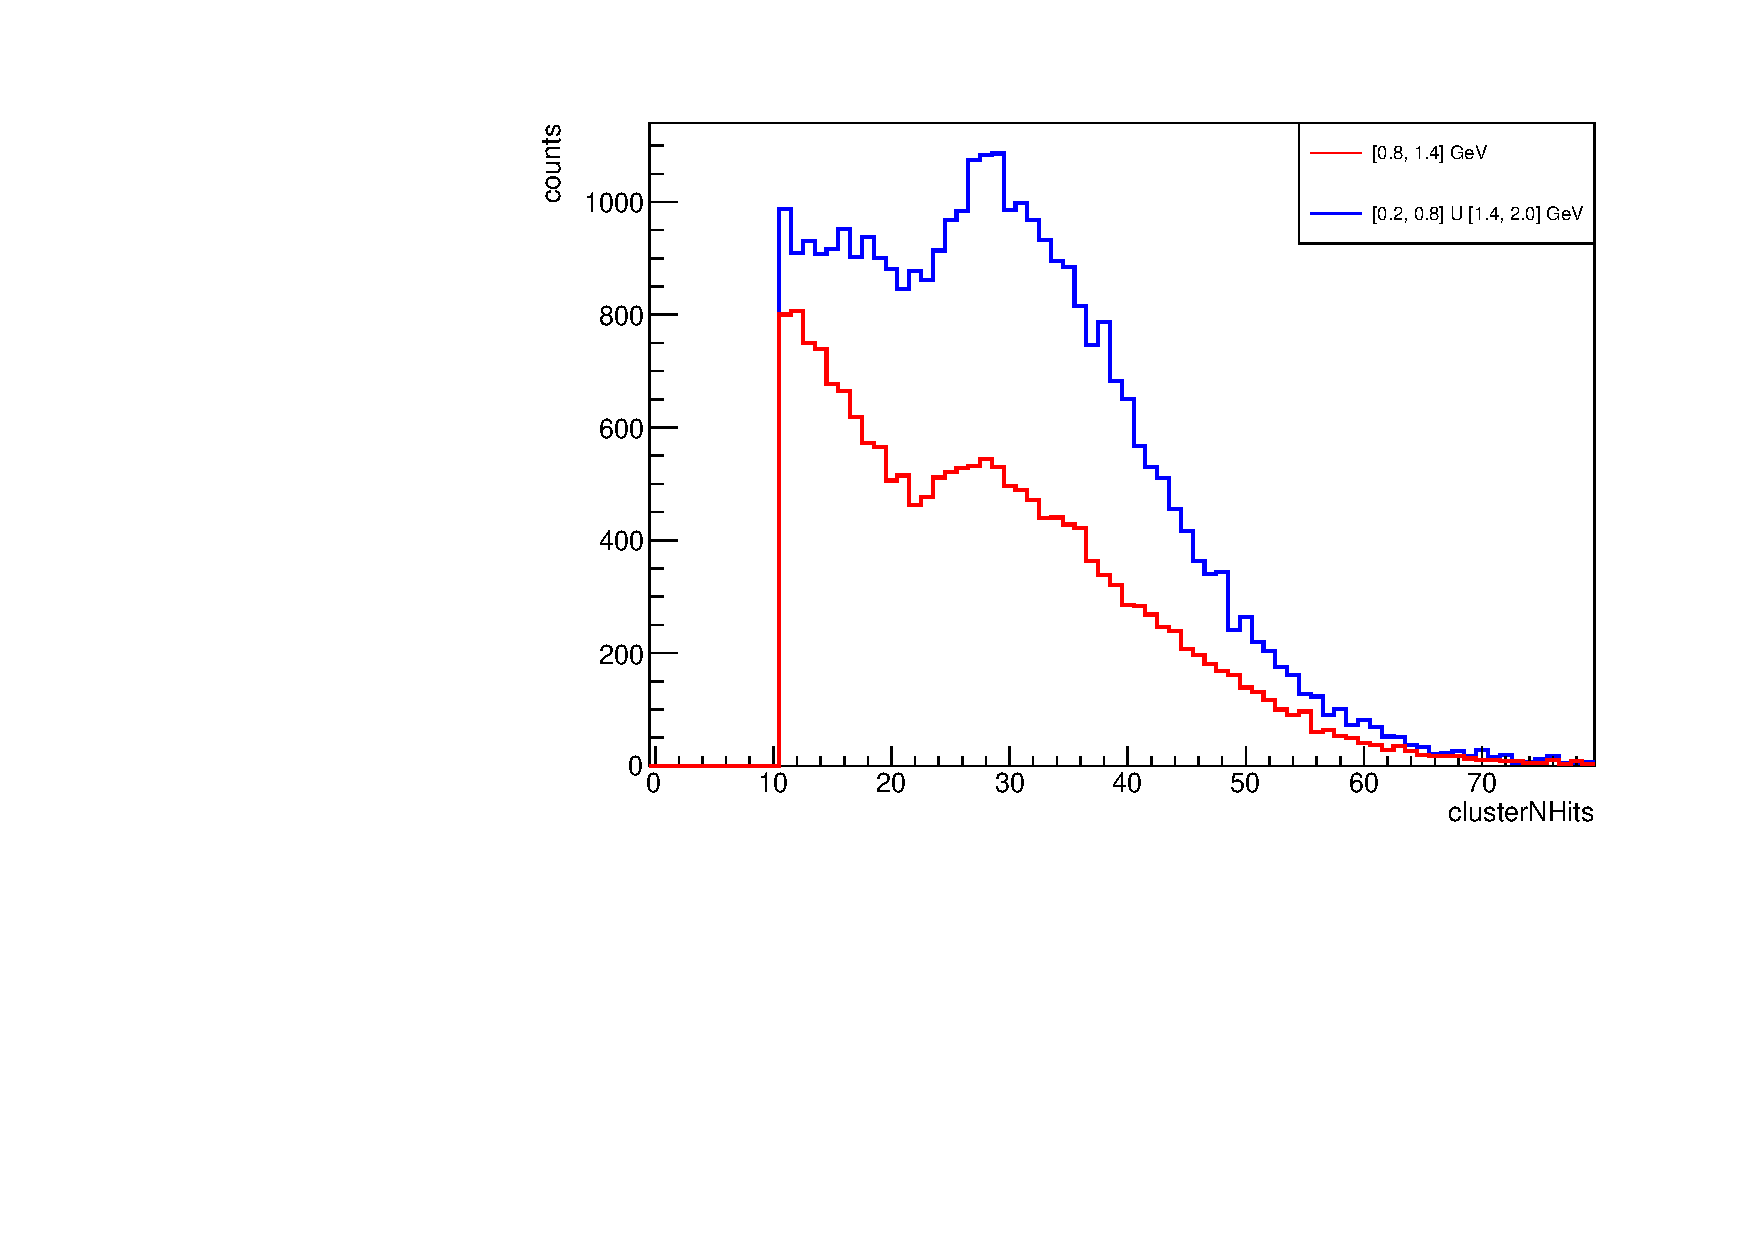
\includegraphics[width=0.49\textwidth]{nbar_cocktail/images/sidebands_clusterNHits_isr.pdf}
     \caption{Comparison of reconstructed cluster variables for $\bar{n}$ candidates in the signal region [0.8, 1.2] GeV (blue) with $\bar{n}$ candidates in the sidebands region [0.3, 0.7] U [1.3, 1.7]  GeV  (red), in NO ISR case. A scaling factor of $k = 0.5$ has been applied to the cluster variables obtained from the sidebands regions. q$\bar{q}$ cocktail. NO ISR case.}
     \label{fig:clus_vars_sidebands_pre_isr}
\end{figure}
Even though the signal is less evident, the same conclusions as in the NO ISR case hold, observing the same kind of structures in the cluster variables distributions, but with more statistic. Therefore, the sidebands regions contribution is now subtracted from the signal region contribution. The obtained cluster variables are shown in Fig.\ref{fig:clus_vars_sidebands_post_isr}.
 \begin{figure}[h]
    \centering
    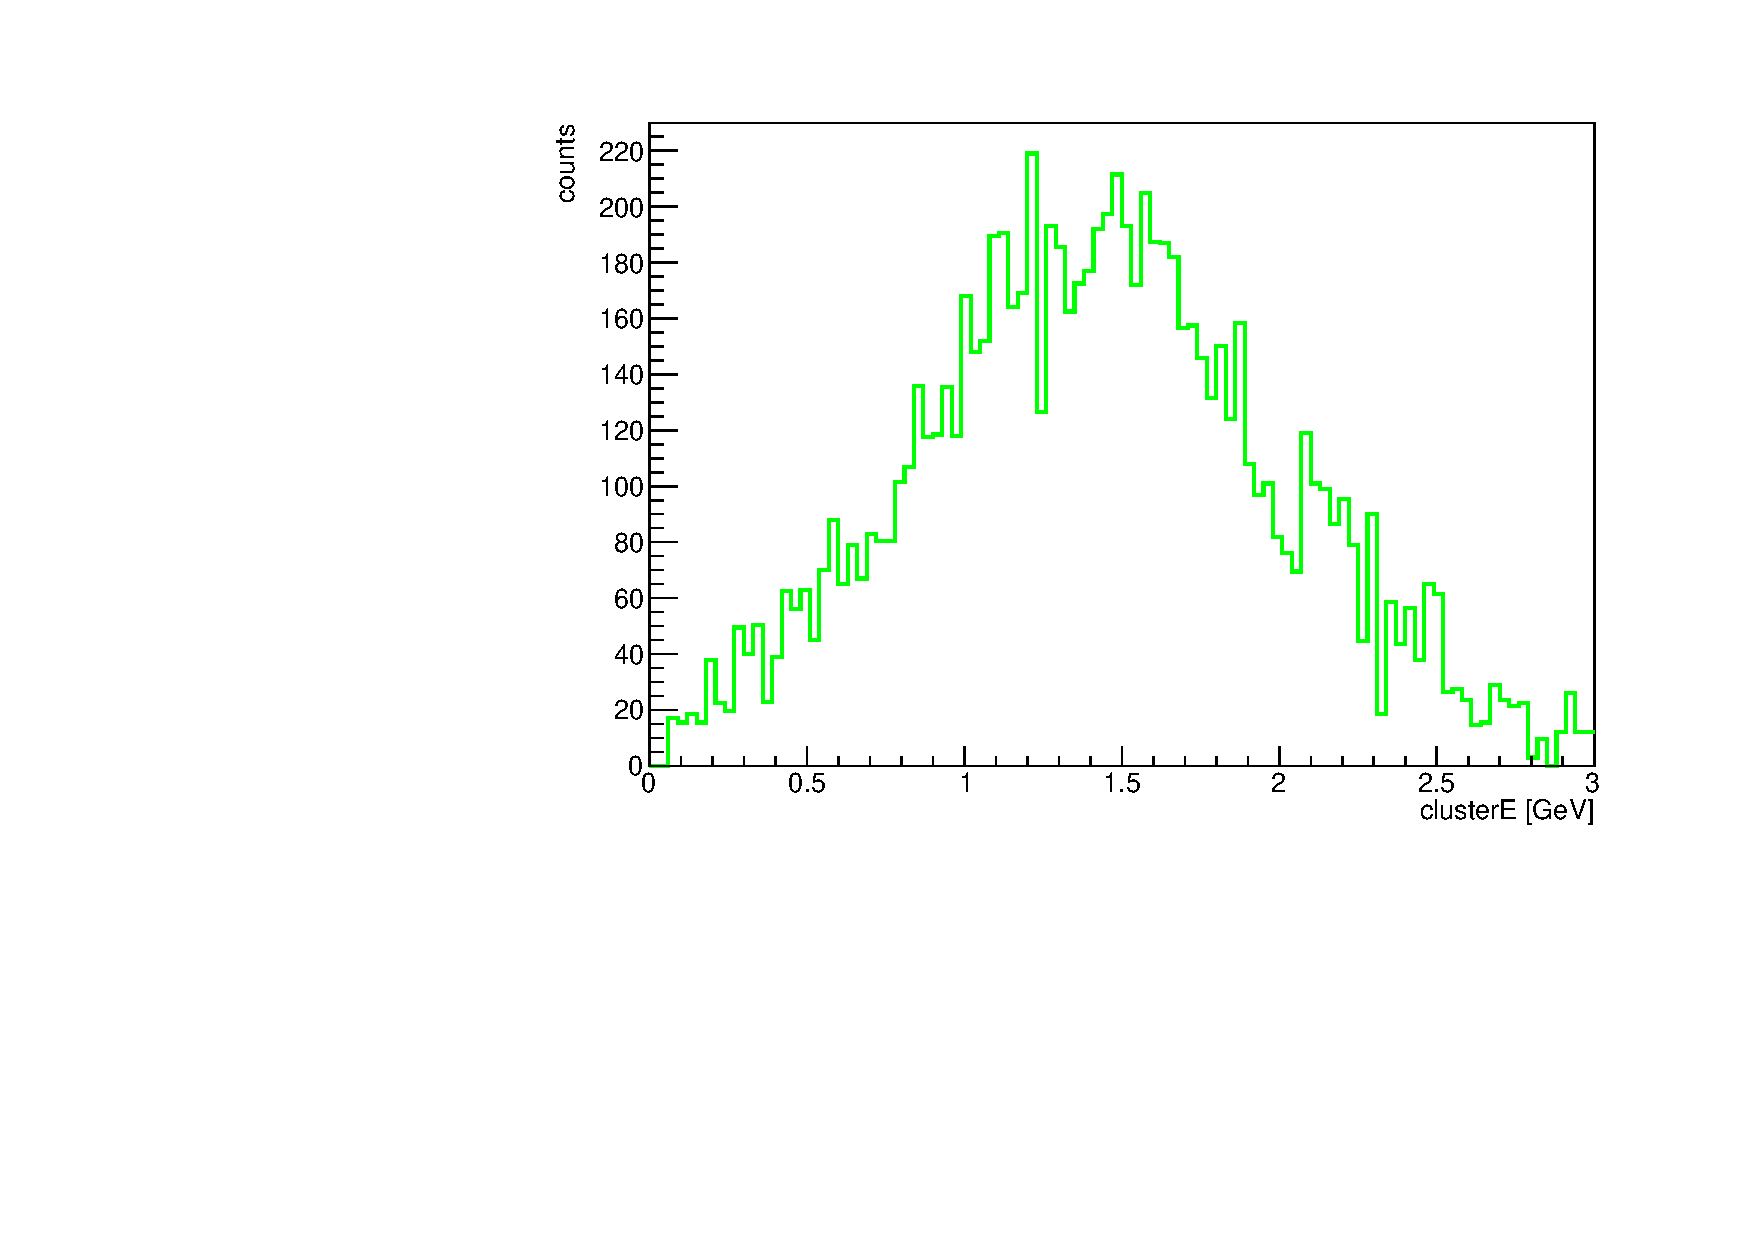
\includegraphics[width=0.49\textwidth]{nbar_cocktail/images/final_clusterE_isr.pdf}
    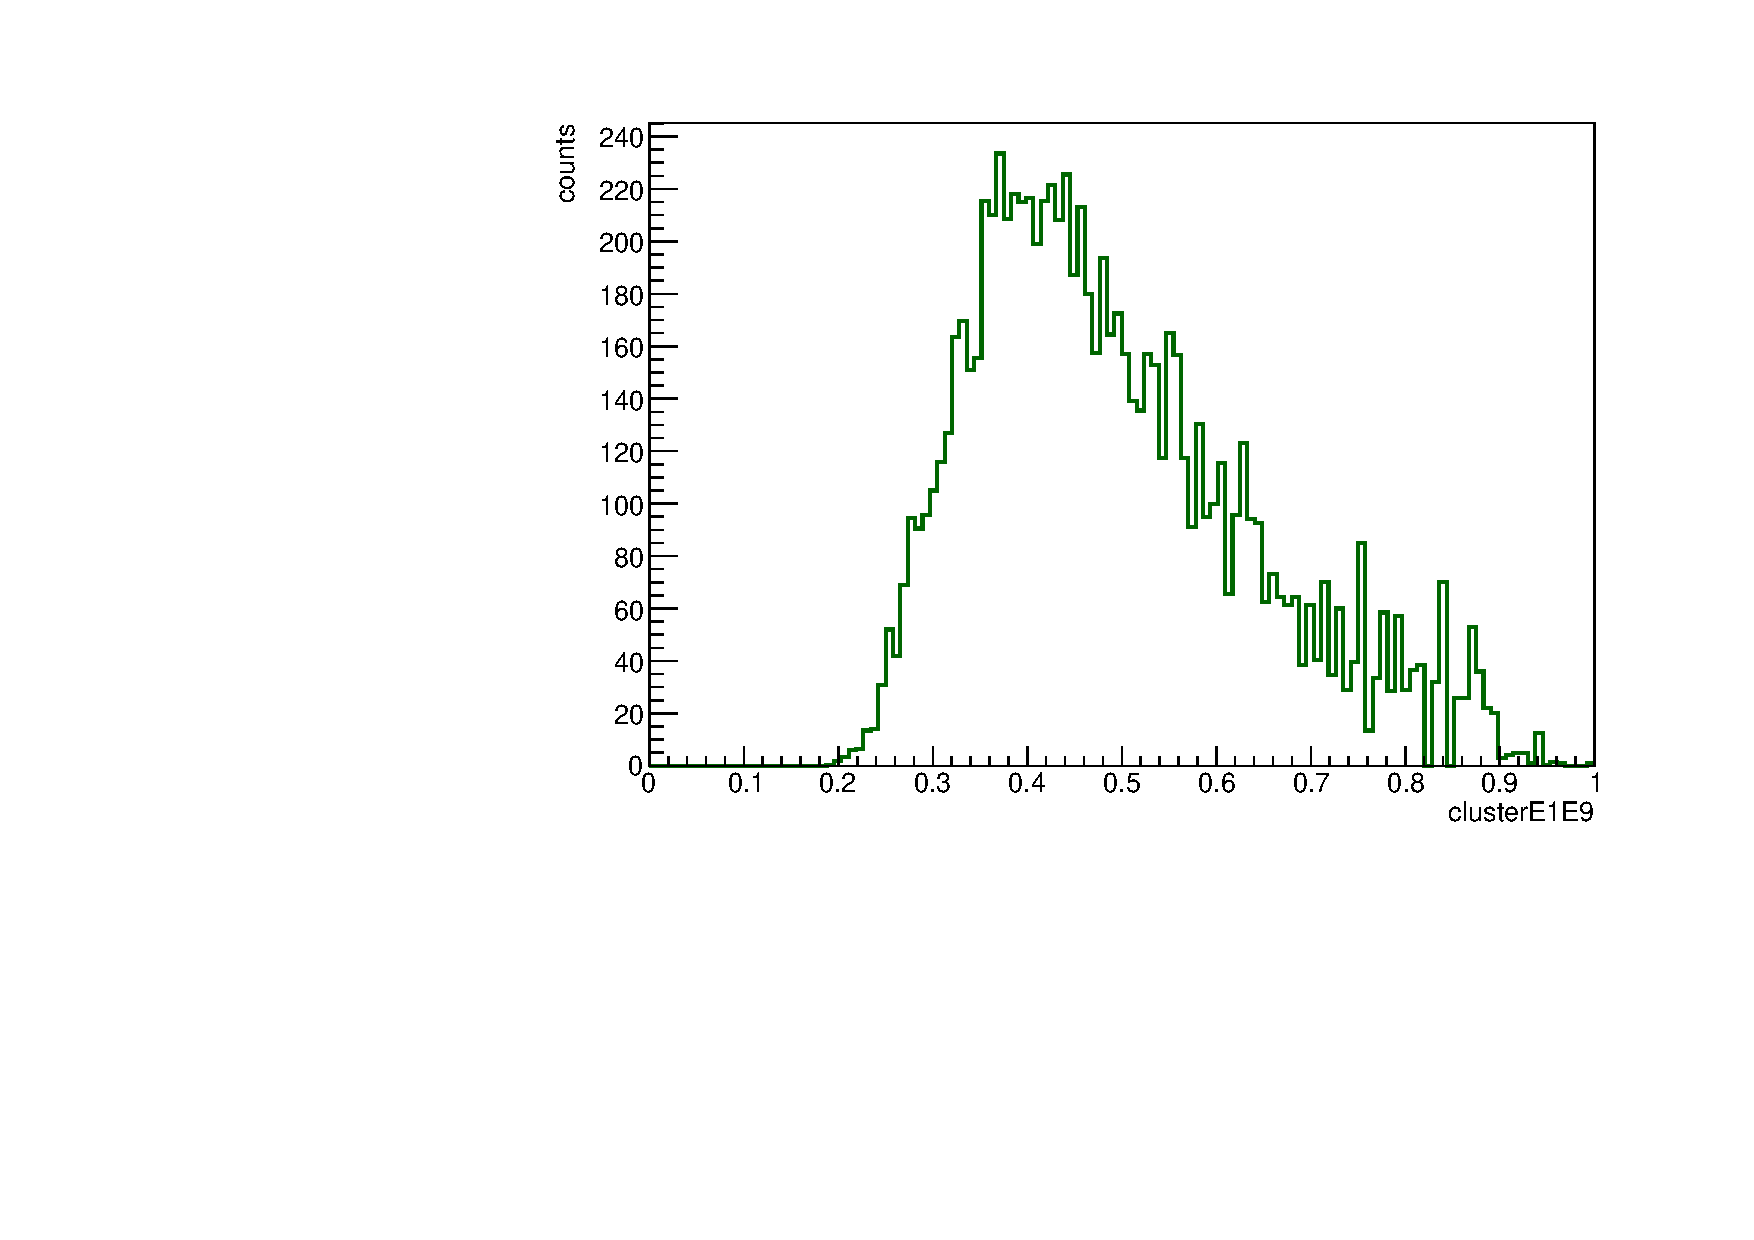
\includegraphics[width=0.49\textwidth]{nbar_cocktail/images/final_clusterE1E9_isr.pdf}
    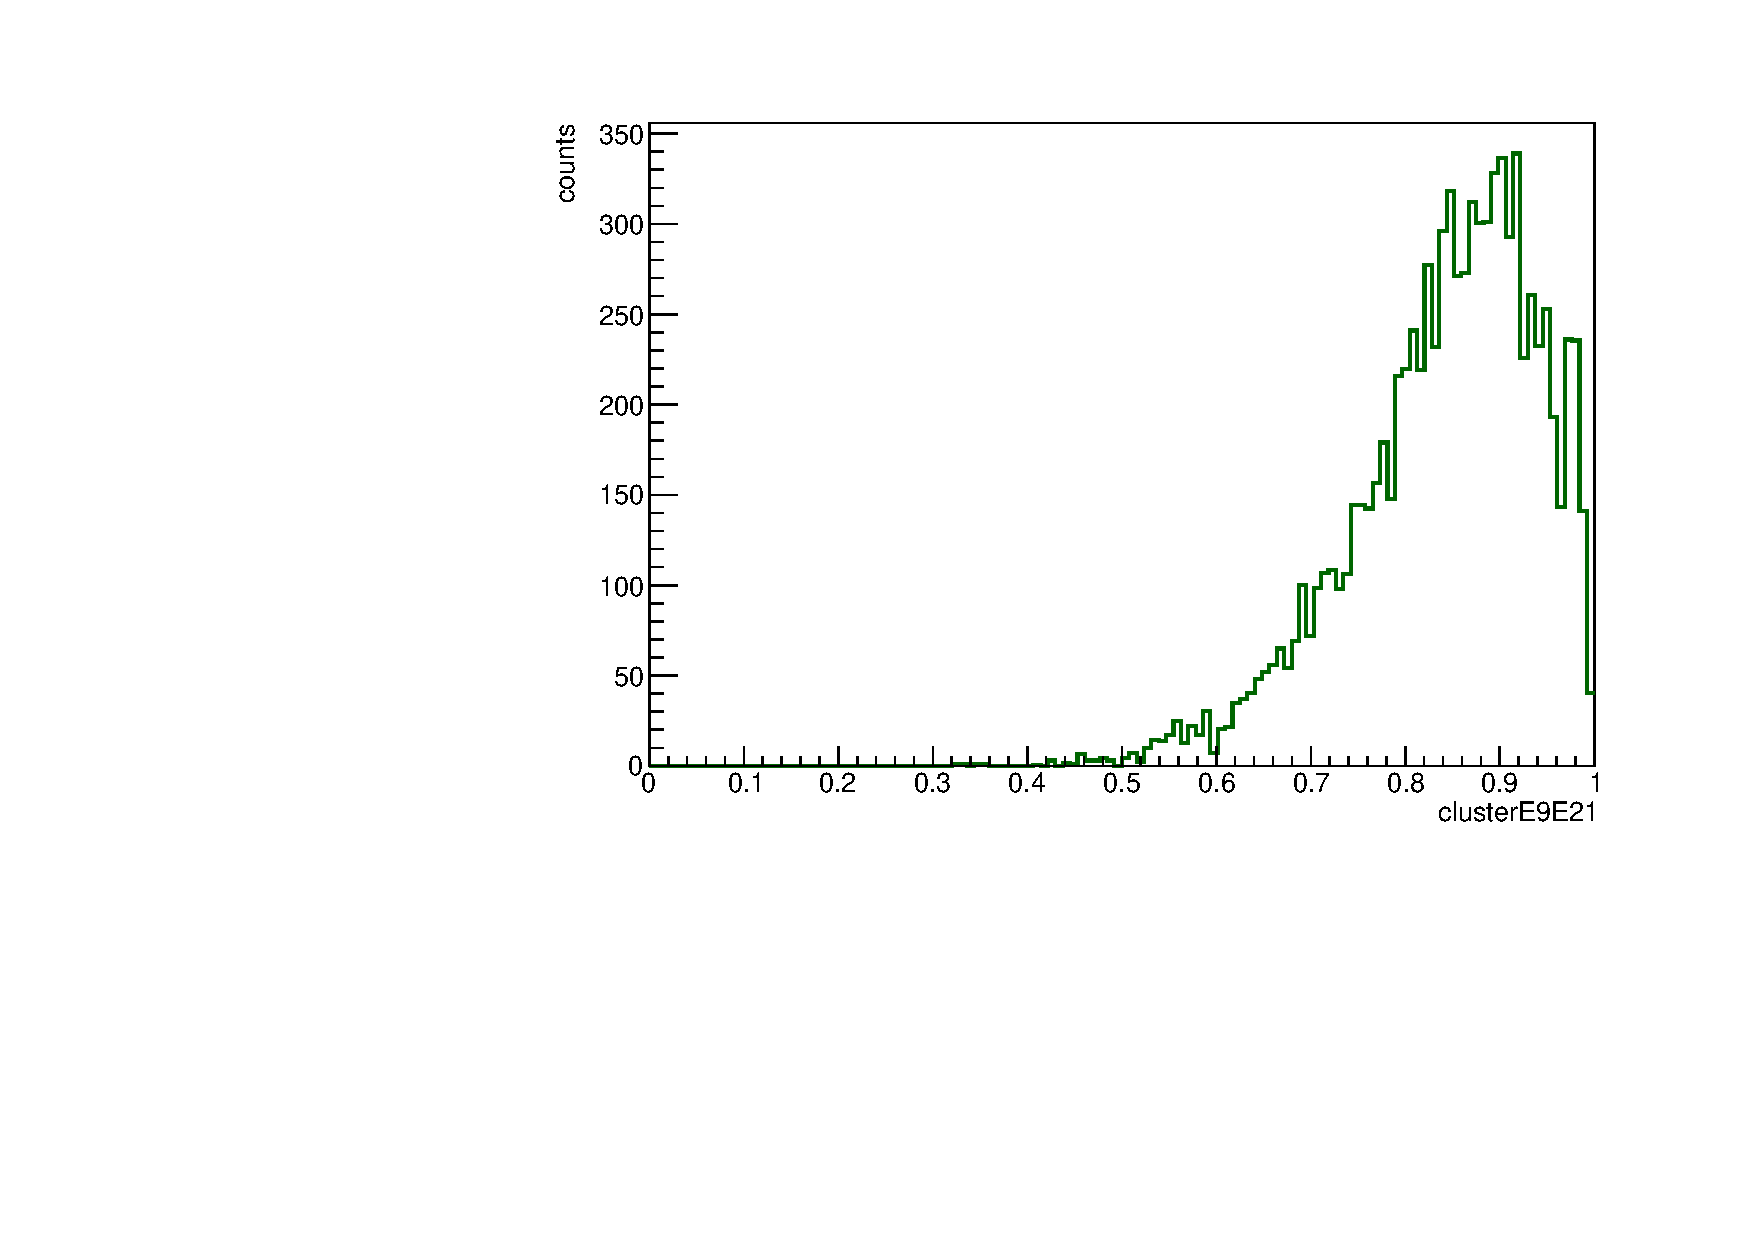
\includegraphics[width=0.49\textwidth]{nbar_cocktail/images/final_clusterE9E21_isr.pdf}
    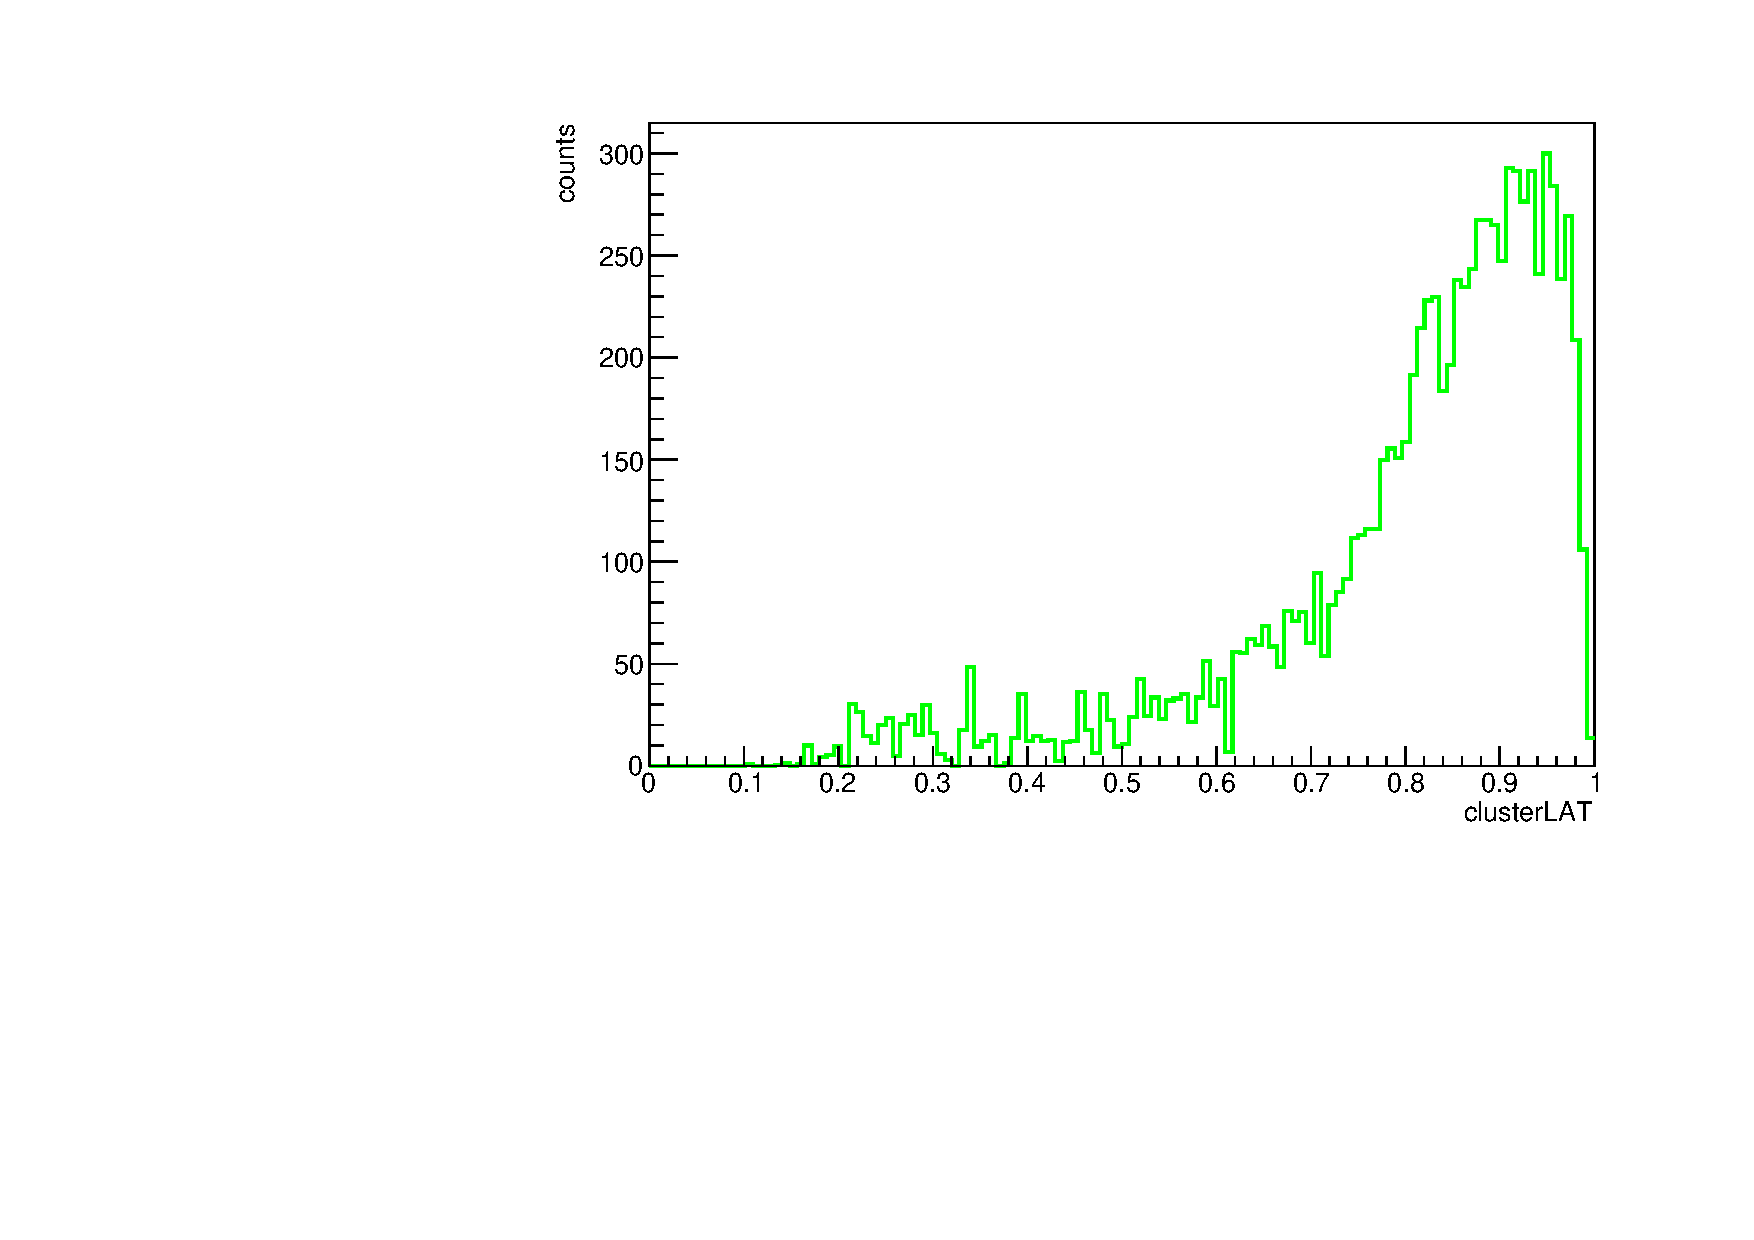
\includegraphics[width=0.49\textwidth]{nbar_cocktail/images/final_clusterLAT_isr.pdf}
    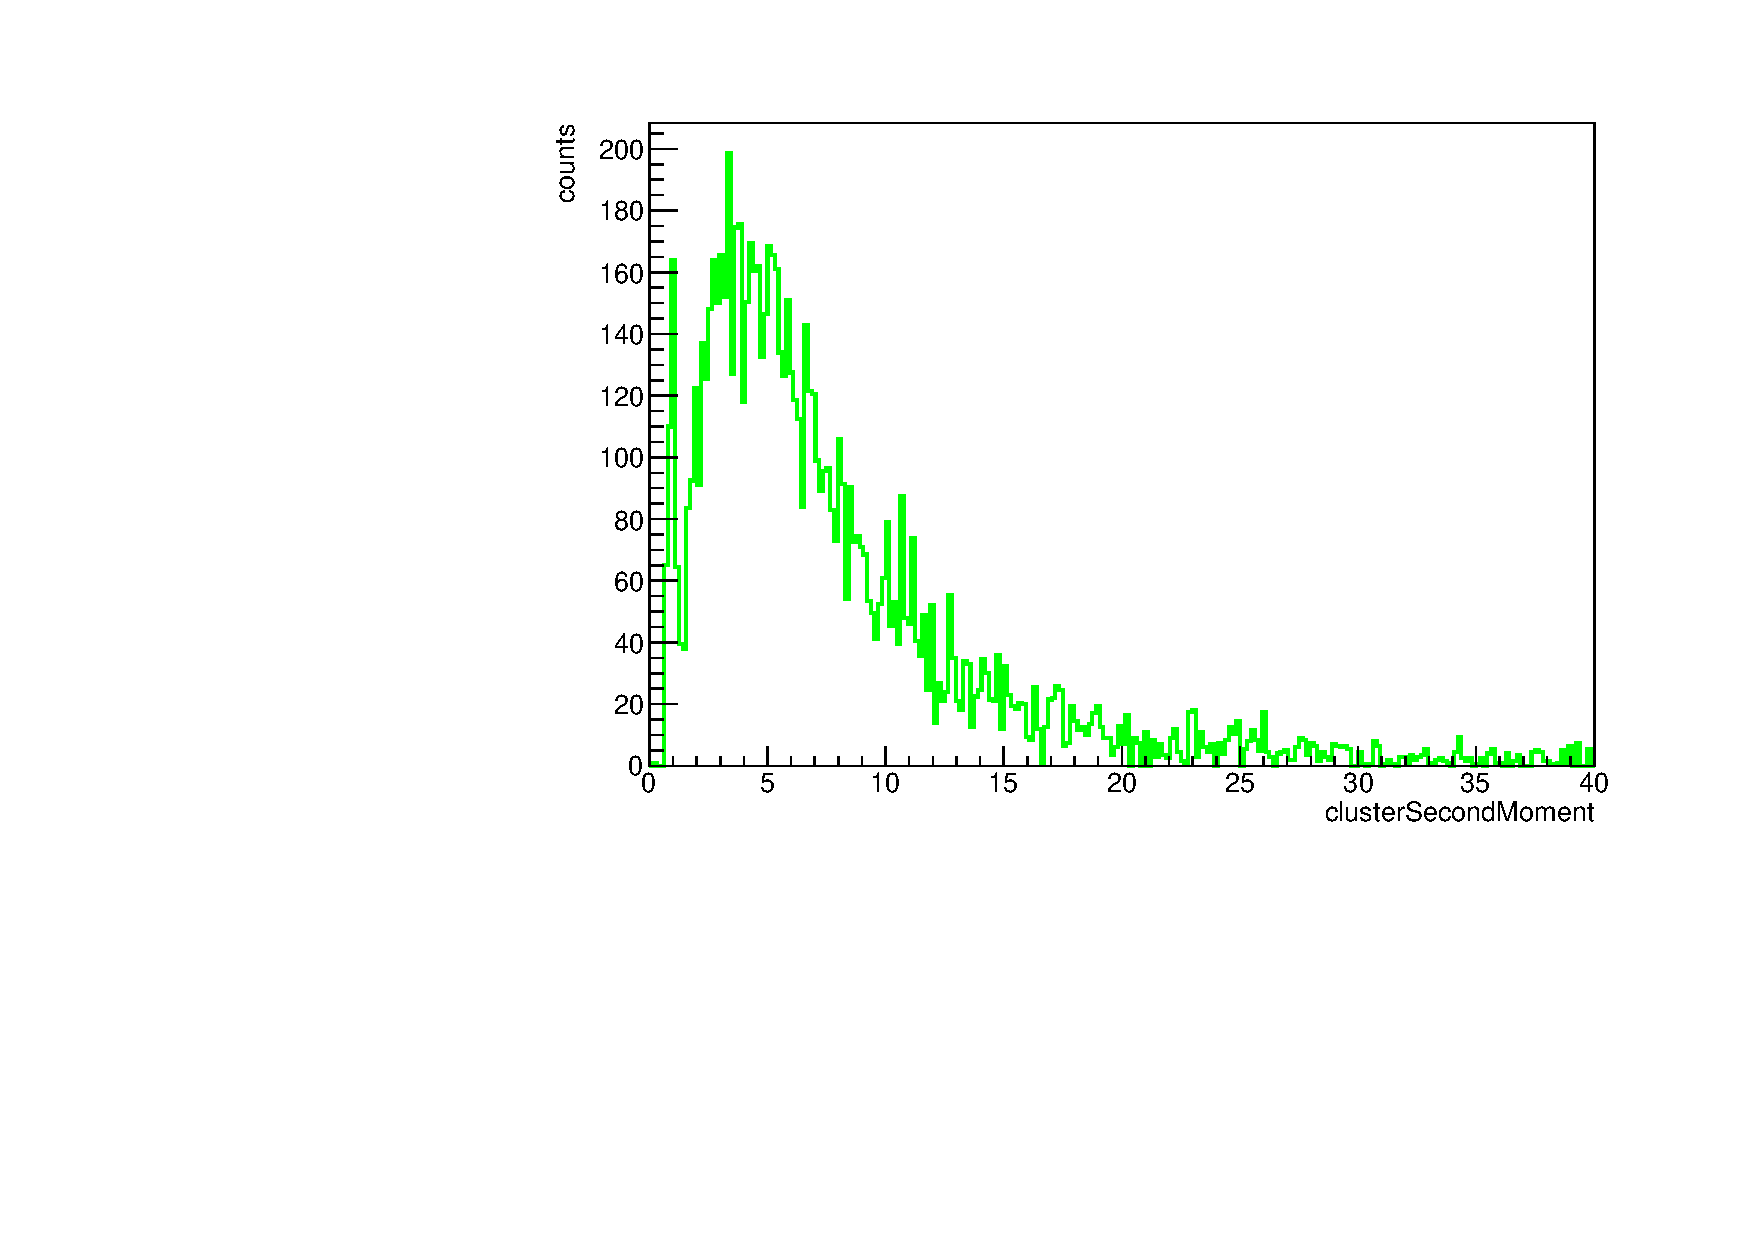
\includegraphics[width=0.49\textwidth]{nbar_cocktail/images/final_clusterSecondMoment_isr.pdf}
    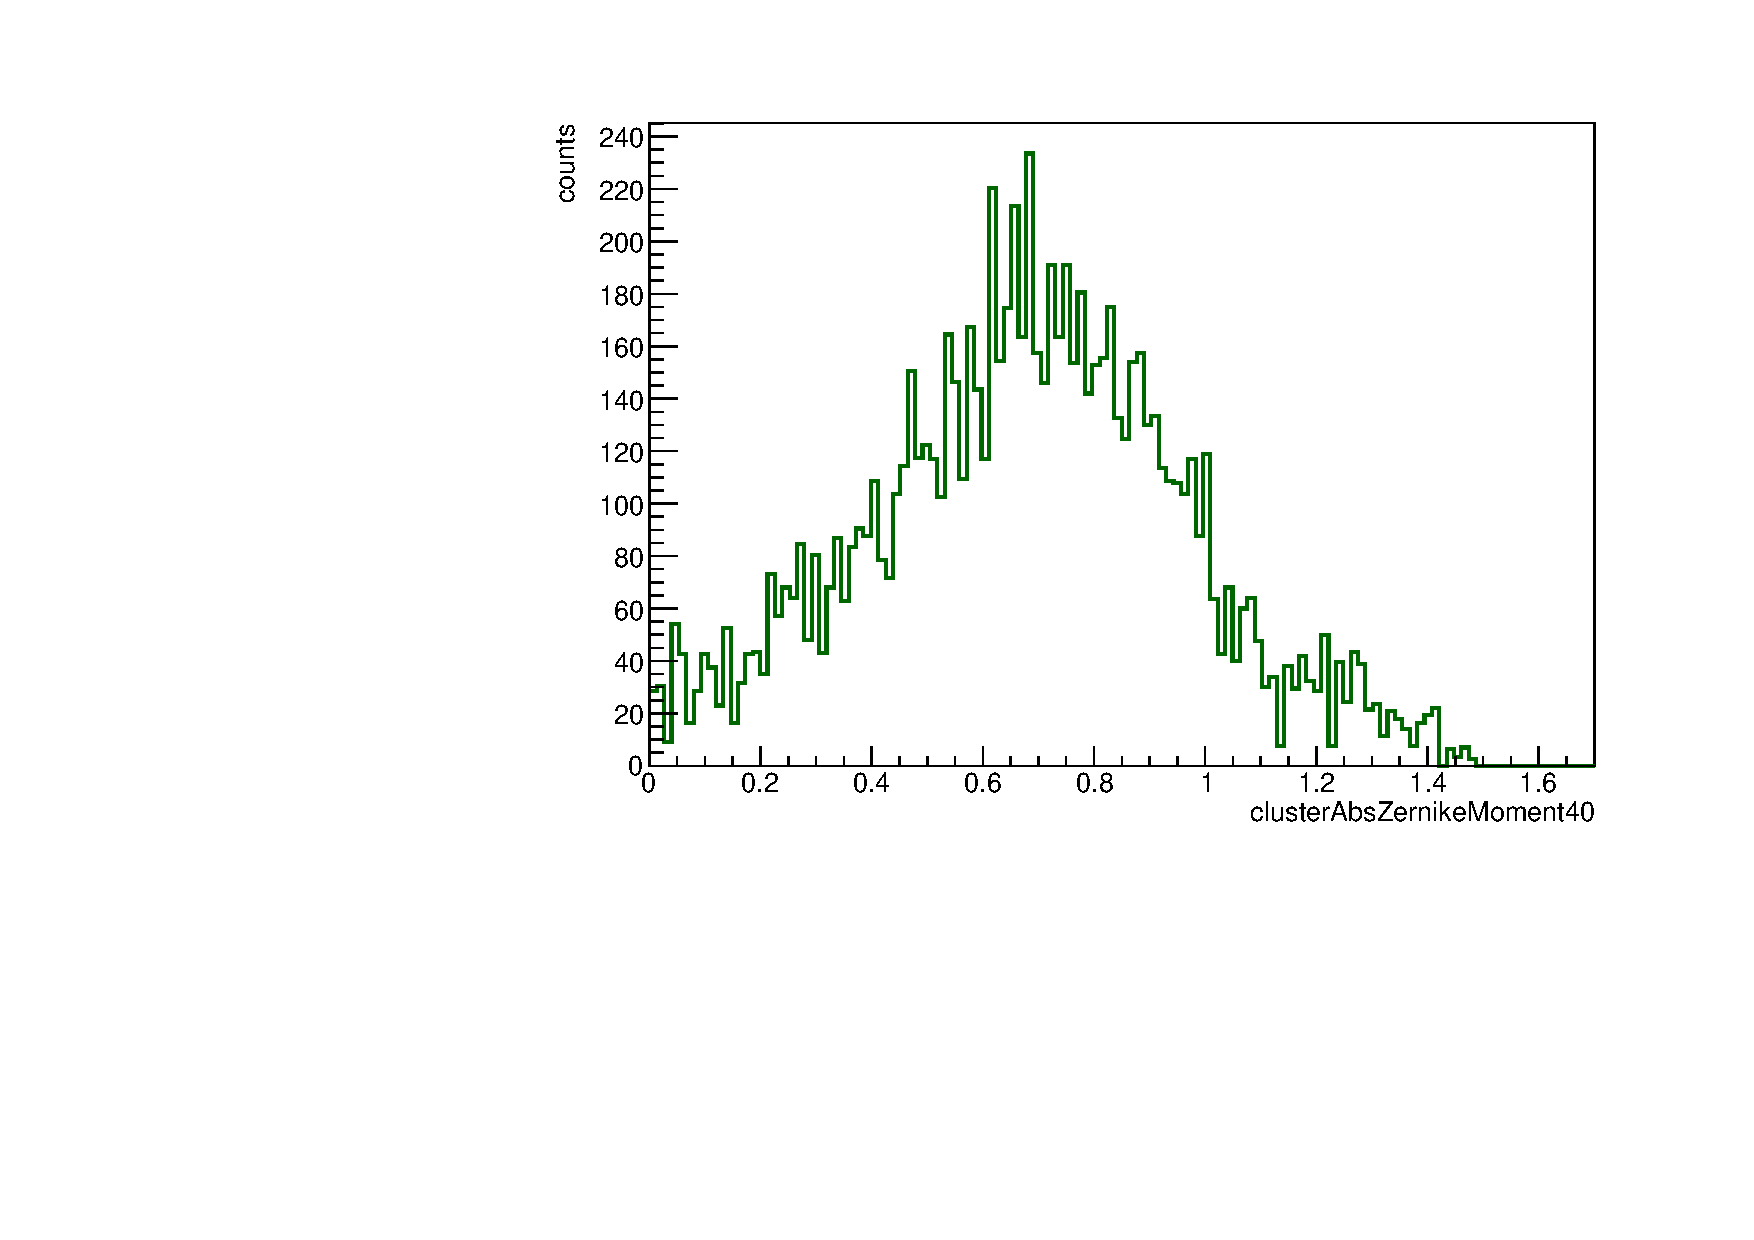
\includegraphics[width=0.49\textwidth]{nbar_cocktail/images/final_clusterAbsZernikeMoment40_isr.pdf}
    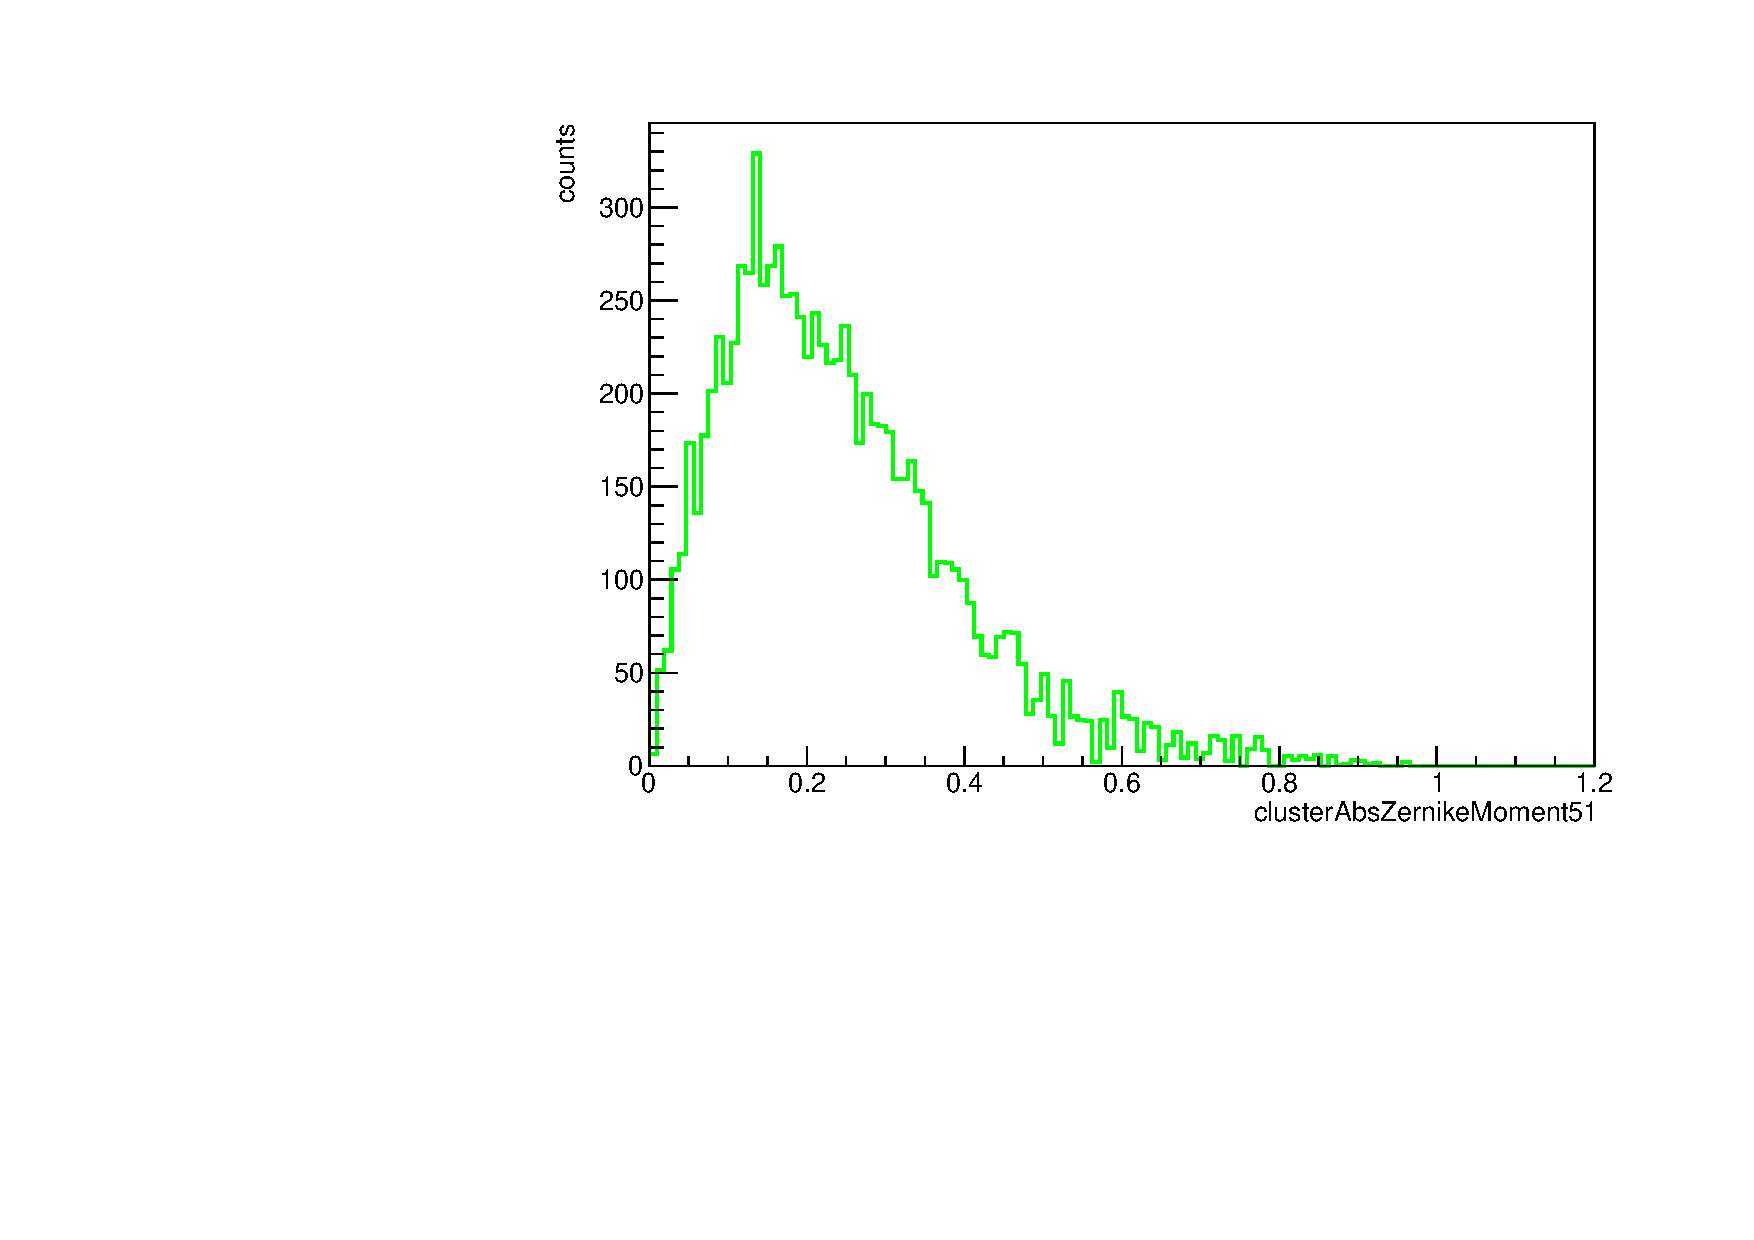
\includegraphics[width=0.49\textwidth]{nbar_cocktail/images/final_clusterAbsZernikeMoment51_isr.pdf}
    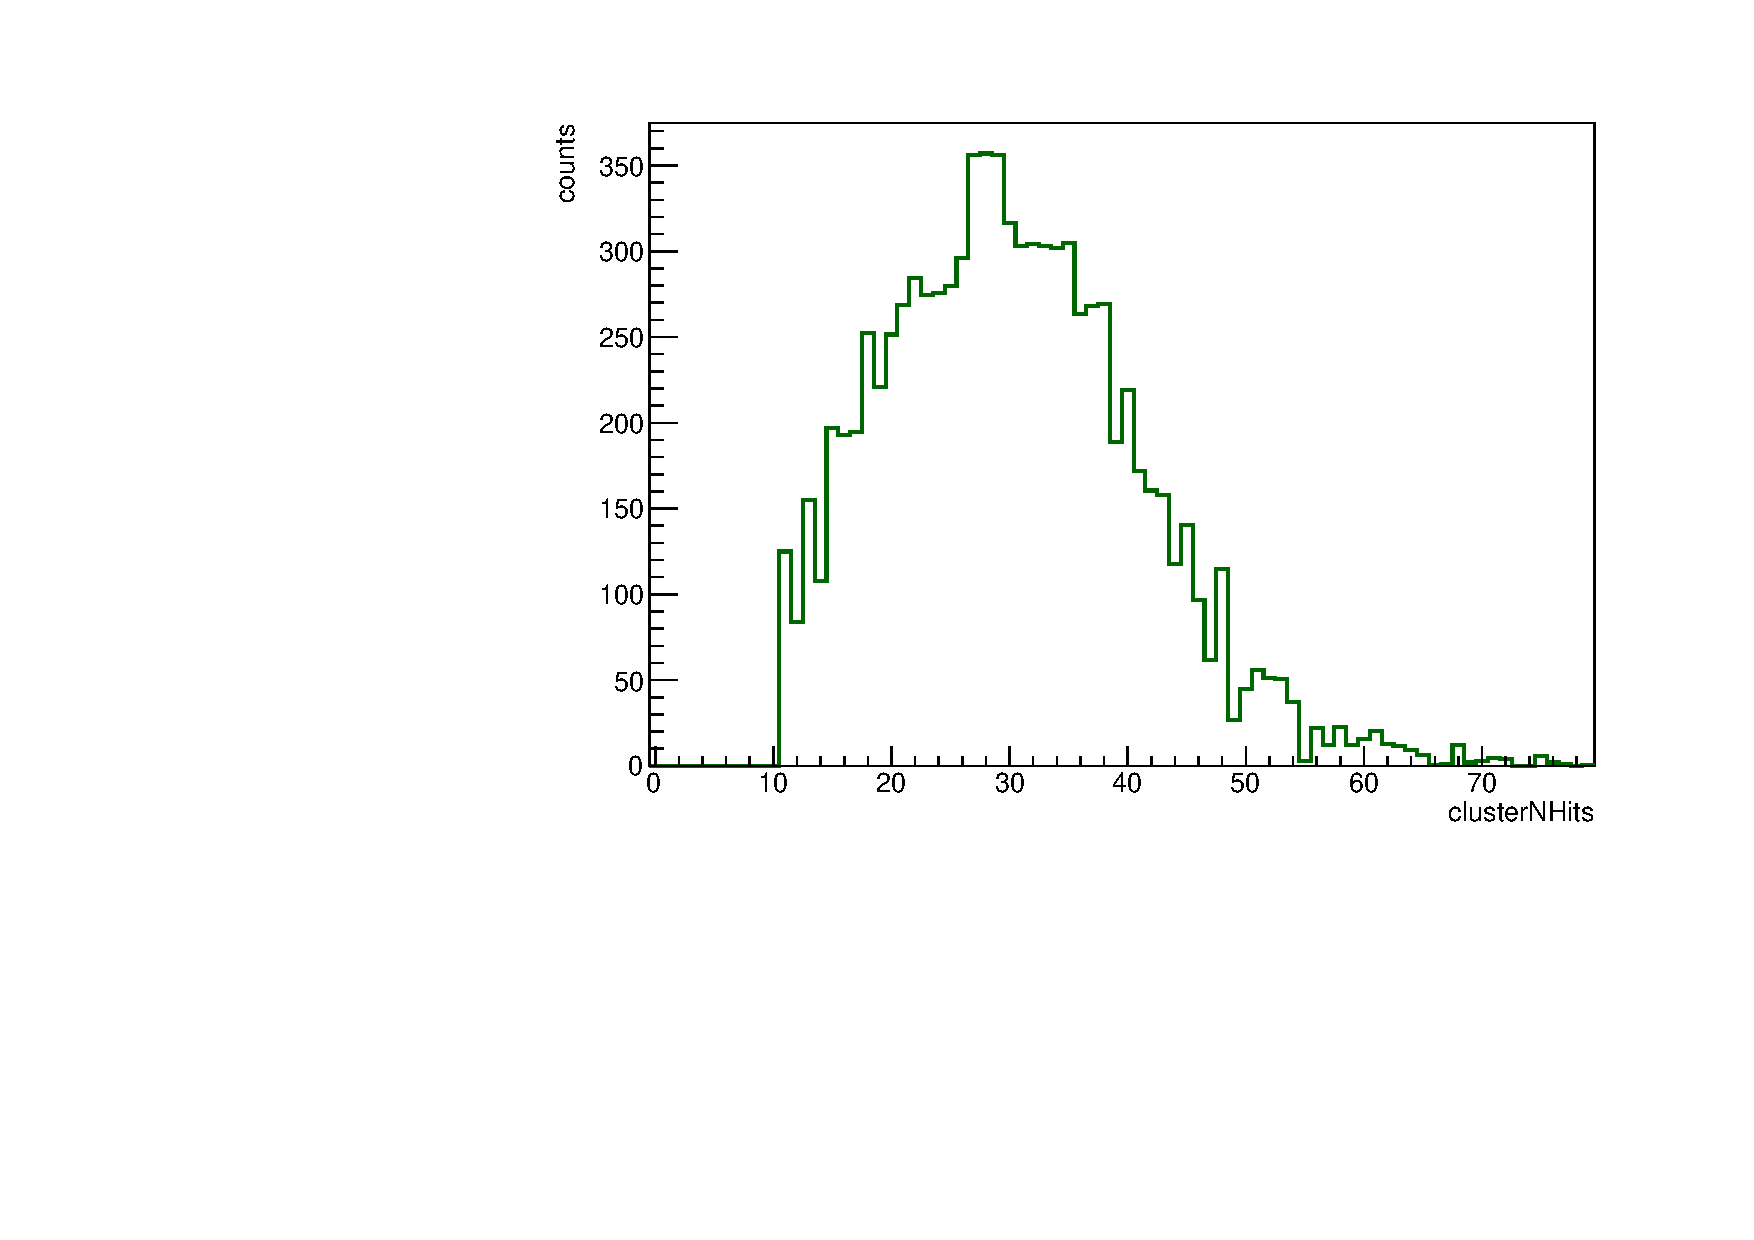
\includegraphics[width=0.49\textwidth]{nbar_cocktail/images/final_clusterNHits_isr.pdf}
   
     \caption{Reconstructed cluster variables for $\bar{n}$ candidates after the application of the sidebands technique, in ISR case. q$\bar{q}$ cocktail.}
     \label{fig:clus_vars_sidebands_post_isr}
\end{figure}
$\\$
As observed in NO ISR case, the obtained cluster variables distributions no longer present the singular structures observed prior to the sidebands technique application, leading to reconstructed cluster variables more similar to those obtained from the Monte Carlo signal sample. 
$\\$
The last step consists in comparing the obtained cluster variables with those obtained from real data, performing the so called \textbf{Data/MC agreement}.

\subsection{Summary of Monte Carlo cocktail Analysis}
The channel $e^+ \ + \  e^- \rightarrow p \ + \ \pi^- \ + \ \bar{n} $ has been studied, with both ISR and NO ISR emission, in $q\bar{q}$ Monte Carlo cocktail.
$\\$
$\\$
A stricter event selection was applied using the Rest of Event (ROE) approach to exclude additional charged tracks outside the signal final state. Furthermore, the $\bar{n}$ candidates energy range was narrowed to reject the main ISR radiation background.
$\\$
$\\$
The recoil mass was then studied in the $u\bar{u}$ cocktail, with a components analysis performed using TopoAna output. This shows that both channels with and without explicit $\gamma_{ISR}$ reconstruction mainly populate the signal region. Performance metrics were then evaluated, optimizing the $\alpha$ angle selection to maximize the figure of merit $\frac{S}{\sqrt{S + B}}$, achieving $\epsilon_{sig} = 90\%$ and $\epsilon_{bkg} = 68\%$ signal-background discrimination power.
$\\$
$\\$
The $q\bar{q}$ cocktail analysis, including recoil mass component decomposition, confirms the findings from the $u\bar{u}$ cocktail. However, in the ISR case, contributions from various channels span the entire recoil mass distribution without specific enhancement in the signal region. Thus, the signal and sideband regions were defined differently than in the NO ISR case.
$\\$
$\\$
Therefore, the $\bar{n}$ candidate cluster variables were studied before and after sidebands subtraction, showing good agreement with signal sample studies. The sidebands technique effectively excluded unexpected structures by removing 
background contributions from cluster variables, in the signal region.